% From https://github.com/UWIT-IAM/UWThesis

\documentclass [11pt, proquest] {uwthesis}[2015/03/03]

% Syntax highlighting #22

%% https://github.com/rstudio/rmarkdown/issues/1649
\newlength{\cslhangindent}
\setlength{\cslhangindent}{1.5em}
\newenvironment{CSLReferences}%
{\setlength{\parindent}{0pt}%
\everypar{\setlength{\hangindent}{\cslhangindent}}\ignorespaces}%
{\par}

% fix for pandoc 1.14
\providecommand{\tightlist}{%
  \setlength{\itemsep}{0pt}\setlength{\parskip}{0pt}}

\newtheorem{theorem}{Jibberish}

%% \bibliography{references}

\hyphenation{mar-gin-al-ia}

%
% ----- apply watermark to every page
% ----- change 'stamp' to 'nostamp'
%------ to omit watermark
%
\usepackage[nostamp]{draftwatermark}
% % Use the following to make modification
\SetWatermarkText{DRAFT}
\SetWatermarkLightness{0.95}

%% for the per mil symbol
\usepackage[nointegrals]{wasysym}

%% something about tables, from https://github.com/ismayc/thesisdown/issues/122
\usepackage{calc}

%% for copyright symbol
\usepackage{textcomp}

%% to allow to rotate pages to landscape
\usepackage{lscape}
%% to adjust table column width
\usepackage{tabularx}

% suppress bottom page numbers on first page of each chapter
% because they overlap with text
\usepackage{etoolbox}
\patchcmd{\chapter}{plain}{empty}{}{}

%% for more attractive tables
\usepackage{booktabs}
\usepackage{longtable}


\usepackage{graphicx}


% Double spacing, if you want it.
% \def\dsp{\def\baselinestretch{2.0}\large\normalsize}
% \dsp

% If the Grad. Division insists that the first paragraph of a section
% be indented (like the others), then include this line:
% \usepackage{indentfirst}

%%%%%%%%%%%%%%%%%%
% If you want to use "sections" to partition your thesis
% un-comment the following:
%
% \counterwithout{section}{chapter}
% \setsecnumdepth{subsubsection}
% \def\sectionmark#1{\markboth{#1}{#1}}
% \def\subsectionmark#1{\markboth{#1}{#1}}
% \renewcommand{\thesection}{\arabic{section}}
% \renewcommand{\thesubsection}{\thesection.\arabic{subsection}}
% \makeatletter
% \let\l@subsection\l@section
% \let\l@section\l@chapter
% \makeatother
%
% \renewcommand{\thetable}{\arabic{table}}
% \renewcommand{\thefigure}{\arabic{figure}}
%
%%%%%%%%%%%%%%%%%%


%% Stuff from https://github.com/suchow/Dissertate

% The following line would print the thesis in a postscript font

% \usepackage{natbib}
% \def\bibpreamble{\protect\addcontentsline{toc}{chapter}{Bibliography}}

\setcounter{tocdepth}{1} % Print the chapter and sections to the toc
% controls depth of table of contents (toc): 0 = chapter, 1 = section, 2 = subsection

\usepackage{biblatex}

\prelimpages

%% from thesisdown
% To pass between YAML and LaTeX the dollar signs are added by CII
\Title{Applied ecosystem chemistry: linking biogeochemical and physiological
processes to ecological interactions}
\Author{Megan L Feddern}
\Year{2021}
\Program{School of Aquatic and Fishery Sciences}
\Chair{Gordon W. Holtgrieve}{Assistant Professor}{School of Aquatic and Fishery Sciences}
\Signature{Eric J. Ward}
\Signature{Tim Essington}
\Signature{Sarah Converse}

% commands and environments needed by pandoc snippets
% extracted from the output of `pandoc -s`
%% Make R markdown code chunks work
\usepackage{array}
\usepackage{amssymb,amsmath}
\usepackage{ifxetex,ifluatex}
\ifxetex
  \usepackage{fontspec,xltxtra,xunicode}
  \defaultfontfeatures{Mapping=tex-text,Scale=MatchLowercase}
\else
  \ifluatex
    \usepackage{fontspec}
    \defaultfontfeatures{Mapping=tex-text,Scale=MatchLowercase}
  \else
    \usepackage[utf8]{inputenc}
  \fi
\fi
\usepackage{color}
\usepackage{fancyvrb}


\ifxetex
  \usepackage[setpagesize=false, % page size defined by xetex
              unicode=false, % unicode breaks when used with xetex
              xetex,
              colorlinks=true,
              linkcolor=blue]{hyperref}
\else
  \usepackage[unicode=true,
              colorlinks=true,
              linkcolor=blue]{hyperref}
\fi
\hypersetup{breaklinks=true, pdfborder={0 0 0}}
\setlength{\parindent}{0pt}
\setlength{\parskip}{6pt plus 2pt minus 1pt}
\setlength{\emergencystretch}{3em}  % prevent overfull lines
\setcounter{secnumdepth}{2} %% controls section numbering, e.g. 1 or 1.2, or 1.2.3

\begin{document}
\copyrightpage

\titlepage

\setcounter{page}{-1}
\abstract{Physical environments are changing globally due to anthropogenic impacts
which have the potential to alter ecological interactions. To understand
how ecological interactions are changing, long-term datasets are
necessary to document ecological baselines from the past that are
comparable to current ecological conditions. Stable isotope values can
be useful chemical tracers for retrospective analyses which can
elucidate changes in biogeochemistry and trophic interactions that
influence food webs. My dissertation applies compound-specific stable
isotope analysis (CSIA) of amino acids and inorganic nitrogen to
understand long-term, regional, ecological responses to physical
conditions in the northeast Pacific. I tested the long-term importance
of salmon subsidies to Alaskan riparian ecosystems by measuring
inorganic nitrogen concentrations, transformation rates, and nitrogen
stable isotope values in soil following a 20-year carcass manipulation
experiment. Carcass subsidies did not increase soil nitrogen
concentrations or transformation rates but the nitrogen stable isotope
value of ammonium was significantly enriched in 15N compared to salmon
carcasses, indicating the importance of salmon derived nutrients is
likely overestimated for some systems. Using museum skull specimens from
two species of pinnipeds in the northeast Pacific, harbor seals
(\emph{Phoca vitulina}) and Steller sea lions (\emph{Eumetopias
jubatus}), I derived a century of predator stable isotope data. I
compared the carbon and nitrogen stable isotope values of source amino
acids to regional climate datasets and determined coastal food webs
responded to climate regimes, coastal upwelling, and freshwater
discharge, yet the strength of responses to individual drivers varied
across the northeast Pacific. These findings demonstrate stable isotope
data can serve as a tracer of nitrogen resources and phytoplankton
dynamics that is specific to resources that are assimilated by food
webs. To calculate pinniped trophic position from the historic dataset,
I was the first to apply taxa-specific trophic enrichment factors, a
system specific beta-value, a temporal lag to account for tissue
turnover time, and a multi-trophic amino acid analysis framework within
a single study. This approach constrained assumptions regarding
physiological processes and vascular plant contributions to the food
web, which can confound stable isotope data interpretation. I analyzed
long-term predictors of harbor seal trophic position in Washington and
identified delayed responses of harbor seals to both physical ocean
conditions (upwelling, sea surface, discharge) and prey availability
(Pacific hake, Pacific herring and Chinook salmon). Consideration for
dynamic responses of harbor seals to their environment is an important
factor for understanding predator-prey interactions as harbor seals
respond to multiple ecological factors that are often changing
simultaneously and their response occurs at multiple temporal scales. I
then analyzed regional and decadal trends in pinniped trophic position
in Alaska and identified the largest change in trophic position occurred
in recent decades (2000 and 2010) but the direction of the trends
diverged based on region and species. Gulf of Alaska pinnipeds are
experiencing unique food web conditions in recent decades compared to
the past likely in response to climate-induced ecological change in the
region. Finally, I constructed a compartment model to explore the effect
of stable isotope heterogeneity and consumer isotope incorporation rates
on consumer trophic position estimates using both bulk stable isotope
analysis and CSIA. Bulk stable isotope analysis produced consistent
errors in trophic position estimates by as much as one trophic level
that were more pronounced in higher trophic level consumers and CSIA was
more accurate than bulk stable isotope analysis. Altogether, these
results show CSIA is a useful tracer for elucidating long-term physical
forcing mechanisms on food webs and incorporating physiological
processes that govern stable isotope fractionation into sampling and
analysis design can uncover forcing mechanisms that would otherwise be
overlooked.}

\tableofcontents
\listoffigures
\listoftables

\acknowledgments{My dissertation research was funded by several grants including
Washington Sea Grant, University of Washington, pursuant to National
Oceanic and Atmospheric Administration (award nos. NA18OAR4170095 and
NA19OAR4170360), and the Joint Institute for the Study of the Atmosphere
and Ocean (JISAO) under NOAA Cooperative Agreement NA15OAR4320063
(contribution no. 2020-1116). I personally was funded by the National
Marine Fisheries Service -Sea Grant Joint Fellowship Program in
Population and Ecosystem Dynamics, the School of Aquatic and Fishery
Sciences Departmental Fellowships, incuding the H. Mason Keeler
Endowment for Excellence and the Clairmont L. and Evelyn S. Egvedt
Fellowship, the American Fisheries Society WA/BC Chapter Jeff Cederholm
Scholarship, and Teaching Assistantship positions.

I extend my deepest gratitude to my museum collaborators for permitting
sampling and coordinating logistics. Specifically, I would like to thank
Jeff Bradley and Sharlene Santana of the UW Burke Museum, Peter
Wimberger and Gary Shugart of the Slater Museum, Link Olson and Aren
Gunderson of the Museum of the North, Robert Delong of the National
Marine Mammal Laboratory, Lesley Kennes and Gavin Hanke of the Royal BC
Museum, and Darrin Lunde and John Ososky of the Smithsonian Institute. I
thank Megan Stachura and Tom Royer for assistance with environmental
datasets, and Chris Harvey and Jens Nielsen for helpful discussions and
support. Hyejoo Ro and Karrin Leazer assisted in laboratory work. Mark
Haught and Terry Rolfe assisted with GC/C/IRMS method development,
maintenance, and troubleshooting.

I thank the Alaska Salmon Program at the University of Washington for
facilitating access to the field siteon Hansen Creek, specifically
Jackie Carter, Katie McElroy, and Max Ramos for help with field sampling
and logistics. The daily surveys and carcass manipulation (by 3-- 5
people) have involved far more individuals than I can name, but I
specifically thank Gregory Buck, Harry Rich, Jr., Curry Cunningham,
Chris Boatright, Jackie Carter, and the undergraduate students in the
Aquatic Ecological Research in Alaska classes.

I am eternally grateful for the community that has supported me over the
past five years. Thank you to my advisor, Gordon Holtgrieve, who
encouraged my eclectic research interests and always supported me in
finding work-life balance. My other committee members --- Drs. Eric
Ward, Sarah Converse, Tim Essington, and Cecilia Bitz --- challenged me
to think about my work broadly, communicate clearly, and think
critically about my analyses. Although they were not officially part of
my committee, Drs. Jens Nielsen at the Alaska Fisheries Science Center,
NOAA and Steve Perakis at the Forest and Rangeland Science Center, USGS,
taught me so much about chemistry, collaboration, and mentoring. Thank
you to to all past and present members of the Holtgrieve Lab for
bringing joy and commiseration to the trials and tribulations of lab
work. My fellow SAFS graduate students have been an important part of my
community, thank you for your support and friendship.

And most importantly, thank you to my parents, brother, and partner.
Your support has meant so much to me!}

\dedication{\begin{center}To my grandmother, Gail Feddern, who has read every publication I have
ever written\end{center}}

\textpages


\chapter*{Introduction}\label{introduction}
\addcontentsline{toc}{chapter}{Introduction}

Anthropogenic climate change will impact nutrient cycles, primary
productivity, and thus ecosystem structure in the world's oceans,
although considerable uncertainty still exists regarding the variability
of these changes and how ecosystems will respond. Changes in primary
production has implications for dependent marine ecosystems, as it
influences abundance and interactions in both adjacent and non-adjacent
trophic levels (Frank, Fisher, \& Leggett,
\protect\hyperlink{ref-Frank2015}{2015}; Ware \& Thomson,
\protect\hyperlink{ref-Ware2005}{2005}; Winder \& Sommer,
\protect\hyperlink{ref-Winder2012}{2012}). This bottom-up control of
marine food webs is expected to reduce fishery yields by as much as 20\%
globally by 2100 due to productivity constraints at lower trophic levels
(J. K. Moore et al., \protect\hyperlink{ref-Moore2018}{2018}). Given
both resource availability and community composition of resources impact
the function and stability of food webs (Narwani \& Mazumder,
\protect\hyperlink{ref-Narwani2012}{2012}) it is likely ecosystem
interactions will change in response to environmentally induced shifts
in resources in the future.

Ecological interactions are a fundamental component to studying the
function and dynamics of ecosystems. Currently, anthropogenic and
climatic changes are altering ecological interactions at a global scale,
thus, understanding how interactions function and how environmental
perturbations will alter interactions is imperative. Studies of
environmental control of food webs are often limited to only examining
low trophic level species (Pershing, Head, Greene, \& Jossi,
\protect\hyperlink{ref-Pershing2010}{2010}), or only include indices of
either primary production or environmental change (E. Chassot, Mélin, Le
Pape, \& Gascuel, \protect\hyperlink{ref-Chassot2007}{2007}; Ware \&
Thomson, \protect\hyperlink{ref-Ware2005}{2005}). Oceanic conditions
such as sea surface temperature, freshwater discharge, wind, and ice
cover, have been linked to abundance and recruitment of many fish
species in the Northeast Pacific (C. J. Cunningham, Westley, \& Adkison,
\protect\hyperlink{ref-Cunningham2018}{2018}; Puerta, Ciannelli,
Rykaczewski, Opiekun, \& Litzow,
\protect\hyperlink{ref-Puerta2019}{2019}; Stachura et al.,
\protect\hyperlink{ref-Stachura2014}{2014}), but studies rarely include
proxies or indicators of either nutrient availability or primary
productivity that enable mechanistic understanding of ecosystem response
to the environment.

Lower trophic levels are sensitive to environmental variation in
bottom-up drivers of productivity (Frank, Petrie, Shackell, \& Choi,
\protect\hyperlink{ref-Frank2006}{2006}; Jennings \& Brander,
\protect\hyperlink{ref-Jennings2010}{2010}; Ware \& Thomson,
\protect\hyperlink{ref-Ware2005}{2005}), but few studies have
demonstrated how the impact of these changes span entire food webs on
long time scales. Additionally, somatic growth of large bodied marine
predators is not continuous and typically occurs on a longer temporal
scale than phytoplankton dynamics making it challenging to link higher
trophic level species to forcing lower in the food web. Similarly,
marine predators can utilize resources at multiple spatiotemporal
scales, creating a challenge for linking species abundance to
independent observations of phytoplankton or nutrient dynamics. How
environmentally induced changes in primary productivity ultimately
influences nutrients available to and assimilated by the food web is
thus poorly understood.

An empirical understanding of food web responses to environmental
drivers requires long time series data that span multiple changes in
climate regimes to decouple natural oscillations with long-term changes
(Hastings et al., \protect\hyperlink{ref-Hastings2018}{2018}; Litzow \&
Ciannelli, \protect\hyperlink{ref-Litzow2007}{2007}; Tallis et al.,
\protect\hyperlink{ref-Tallis2010}{2010}). In recent decades extreme
changes in marine environments have become more common and these events
have had substantial impacts on ecosystems. Marine ecosystems in Alaska
are experiencing unprecedented environmental change that has altered
abundance and size distributions of many fish species (Barbeaux,
Holsman, \& Zador, \protect\hyperlink{ref-Barbeaux2020}{2020}; K. K.
Holsman, Aydin, Sullivan, Hurst, \& Kruse,
\protect\hyperlink{ref-Holsman2019}{2019}; Oke et al.,
\protect\hyperlink{ref-Oke2020}{2020}; Suryan et al.,
\protect\hyperlink{ref-Suryan2021}{2021}). More recently, atmospheric
circulation anomalies in the northeast Pacific Ocean have resulted in
abnormally warm sea surface temperatures during the past decade (Walsh
et al., \protect\hyperlink{ref-Walsh2018}{2018}) and this environmental
shift has altered fish abundances (N. A. Bond, Cronin, Freeland, \&
Mantua, \protect\hyperlink{ref-Bond2015}{2015}; Litzow et al.,
\protect\hyperlink{ref-Litzow2020}{2020}). For example, the
unprecedented marine heatwave that occurred in 2014 - 2016 triggered
dramatic ecosystem change, including a 71\% decline in Pacific cod in
the Gulf of Alaska (Barbeaux et al.,
\protect\hyperlink{ref-Barbeaux2020}{2020}) and declines in
phytoplankton biomass, forage fish abundance, and changes in community
structure (Suryan et al., \protect\hyperlink{ref-Suryan2021}{2021}).

Reconstructing time series of indicators of ecosystem interactions is
important to understand how ecosystems have responded to environmental
variability in the past and ultimately interpret potential food web
responses to environmental conditions in the future; such datasets are
distinctly lacking. Modern chemical analyses, such as compound-specific
stable isotope analysis (CSIA) of inorganic nitrogen sources or amino
acids, have potential to improve our understanding of food web
interactions by 1) extending time series through retrospective analyses
2) identifying environmental forcing of the entire food web when
measured in predators and 3) informing biologically relevant mechanisms
of interactions, a former limitation of many ecosystem studies.

Analyses of nitrogen stable isotopes usually applies bulk stable isotope
techniques which measures the \(^{15}N/^{14}N\) ratio of nitrogen as a
weighted average of all nitrogen present in a given sample. For tissue
samples, \(^{15}N/^{14}N\) measurements are a weighted average of the
concentrations of all amino acids present in the protein of an
individual tissue. For soil analyses, typically \(^{15}N/^{14}N\)
includes both organic and inorganic form. However, the \(^{15}N/^{14}N\)
of an individual compound, known as compound-specific stable isotope
analysis, represents the kinetic and diffusive fractionation factors
exerted on that compound through chemical conversions, typically from
biogeochemical or physiological processes. Thus, nitrogen isotope values
can provide a useful link between biogeochemical reactions that regulate
nutrient availability and primary production, and ecological responses,
without being confounded by nitrogen containing compounds that are not
utilized by an ecosystem.

Here I aim to reconstruct historical food web interactions using stable
isotopes as chemical tracers to:
\begin{enumerate}
\def\labelenumi{\arabic{enumi}.}
\item
  Identify how long-term (20-years) changes in salmon abundance impact
  nitrogen dynamics in riparian soils.
\item
  Understand the how ocean conditions alter food web-assimilated
  nitrogen resources and primary production in the northeast Pacific.
\item
  Identify dominant historical drivers of predator trophic position in
  the northeast Pacific, using trophic position as an indicator of major
  changes in food web dynamics and ecological interactions.
\item
  Establish a framework to improve trophic position estimation of bulk
  and compound-specific stable isotope analysis for historical and
  contemporary studies.
\end{enumerate}
\chapter{Riparian soil nitrogen cycling and isotopic enrichment in
response to a long-term salmon carcass manipulation
experiment}\label{riparian-soil-nitrogen-cycling-and-isotopic-enrichment-in-response-to-a-long-term-salmon-carcass-manipulation-experiment}

A version of this chapter was published as: Feddern, M. L., Holtgrieve,
G.W., Perakis, S. S., Hart, J., Ro, H., \& Quinn, T. P. (2019). Riparian
soil nitrogen cycling and isotopic enrichment in response to a long-term
salmon carcass manipulation experiment. Ecosphere, 610(11): e02958.
\url{https://doi.org/10.1002/ecs2.2958}

\section{Abstract}\label{abstract}

Pacific salmon acquire most of their biomass in the ocean before
returning to spawn and die in coastal streams and lakes, thus providing
subsidies of marine-derived nitrogen (MDN) to freshwater and terrestrial
ecosystems. Recent declines in salmon abundance have raised questions of
whether managers should mitigate for losses of salmon MDN subsidies. To
test the long-term importance of salmon subsidies to riparian ecosystems
we measured soil N cycling in response to a 20-year manipulation where
salmon carcasses were systematically removed from one bank and deposited
on the opposite bank along a 2 km stream in southwestern Alaska. Soil
samples were taken at different distances from the stream bank along
nine paired transects and measured for organic and inorganic nitrogen
concentrations, and nitrogen transformation rates. MDN was measured
using \textsuperscript{15}N/\textsuperscript{14}N for bulk soils, and
NH\textsubscript{4}\textsuperscript{+} and
NO\textsubscript{3}\textsuperscript{-} soil pools. Stable isotope
analyses confirmed \textsuperscript{15}N/\textsuperscript{14}N was
elevated on the salmon enhanced bank compared to the salmon depleted
bank. However, \textsuperscript{15}N/\textsuperscript{14}N values of
plant-available inorganic nitrogen exceeded the
\textsuperscript{15}N/\textsuperscript{14}N of salmon inputs,
highlighting N isotope fractionation in soils that raises significant
methodological issues with standard MDN assessments in riparian systems.
Surprisingly, despite 20 years of salmon supplementation, the presence
of MDN did not cause a long-term increase in soil N availability. This
finding indicates the importance of MDN to ecosystem N biogeochemistry
and riparian vegetation may be overestimated for some systems. Given
that essential nutrients can also be pollutants, we urge more critical
analyses of the role of MDN to inform compensatory mitigation programs
targeting salmon nutrient enhancement.

\section{Introduction}\label{introduction-1}

Pacific salmon (\emph{Oncorhynchus spp.}) migration from marine
environments to freshwater spawning grounds is a textbook case of
cross-ecosystem nutrient subsidies, and dozens of studies have
identified the presence of marine-derived nitrogen (MDN) from salmon as
crossing ecosystem boundaries from oceans to freshwaters and into the
terrestrial environment (sensu, (Polis, Power, \& Huxel,
\protect\hyperlink{ref-Polis2004}{2004}; Schindler et al.,
\protect\hyperlink{ref-Schindler2003}{2003}; Scott M, Richard T, Mary F,
\& Mark S, \protect\hyperlink{ref-Gende2002}{2002}). Declines in Pacific
salmon populations in many areas, caused by human activities
(overharvest, habitat degradation, dams) (Richard et al.,
\protect\hyperlink{ref-Gustafson2007}{2007}), and the concern over loss
of MDN to coastal watersheds has made restoration of salmon nutrients a
focal point for many management and mitigation strategies. For example,
in the Columbia River Basin where Pacific salmon populations have
declined, legislation requiring compensatory mitigation has led to
nutrient enhancement programs, on the foundation that habitats have lost
critical nutrients from salmon and therefore augmentation is necessary
to maintain ecosystem function (Collins, Marcarelli, Baxter, \& Wipfli,
\protect\hyperlink{ref-Collins2015}{2015}).

Salmon bring nutrients, including phosphorus (P) and other compounds in
addition to nitrogen (N), into freshwater and terrestrial food webs
through two pathways: 1) direct consumption of tissues by predators and
scavengers, and 2) autotrophic or heterotrophic assimilation of
nutrients released as salmon spawn, die, and eventually decay (Scott M
et al., \protect\hyperlink{ref-Gende2002}{2002}). Salmon are enriched in
the heavy isotope of nitrogen (\textsuperscript{15}N) relative to the
light isotope (\textsuperscript{14}N) when compared to terrestrial and
watershed-derived N. This isotopic enrichment has been used to
quantitatively trace the presence of salmon derived nutrients into
watersheds (Schindler et al.,
\protect\hyperlink{ref-Schindler2003}{2003}). For example, the
proportion of N derived from salmon ranges from approximately 30\% --
75\% in fish and aquatic invertebrates (Naiman, Bilby, Schindler, \&
Helfield, \protect\hyperlink{ref-Naiman2002}{2002}), 10 -- 90\% in
piscivorous mammals such as bears, and 20 -- 40\% in piscivorous fishes
near salmon spawning grounds (Bilby, Fransen, \& Bisson,
\protect\hyperlink{ref-Bilby1996}{1996}; Chaloner, Martin, Wipfli,
Ostrom, \& Lamberti, \protect\hyperlink{ref-Chaloner2002}{2002};
Claeson, Li, Compton, \& Bisson,
\protect\hyperlink{ref-Claeson2006}{2006}; Hilderbrand et al.,
\protect\hyperlink{ref-Hilderbrand1999}{1999}).

The annual return of this predictable and abundant, yet temporally
limited, high quality resource drives the foraging ecology of both
terrestrial and aquatic consumers (Quinn, Helfield, Austin, Hovel, \&
Bunn, \protect\hyperlink{ref-Quinn2018}{2018}; Schindler et al.,
\protect\hyperlink{ref-Schindler2013}{2013}). Carcasses and roe are
documented food sources for over 22 species of mammals, birds (C. J.
Cederholm, Houston, Cole, \& Scarlett,
\protect\hyperlink{ref-Cederholm1989}{1989}), fishes (Scheuerell, Moore,
Schindler, \& Harvey, \protect\hyperlink{ref-Scheuerell2007}{2007}), and
invertebrates (Meehan, Seminet-Reneau, \& Quinn,
\protect\hyperlink{ref-Meehan2005}{2005}; Winder, Schindler, Moore,
Johnson, \& Palen, \protect\hyperlink{ref-Winder2005}{2005}). Bear
population density, body size, and reproductive output has been
correlated with meat (primarily salmon) consumption, with piscivorous
populations having 55 times higher density than their meat-limited
counterparts (Hilderbrand et al.,
\protect\hyperlink{ref-Hilderbrand1999}{1999}). In aquatic ecosystems,
salmon carcass abundance has been correlated with elevated growth rates
of invertebrates, and with size, density, and condition factor of
juvenile salmonids (R. E. Bilby, Fransen, Bisson, \& Walter,
\protect\hyperlink{ref-Bilby1998}{1998}; Wipfli, Hudson, Caouette, \&
Chaloner, \protect\hyperlink{ref-Wipfli2003}{2003}).

The presence of MDN has been documented in aquatic primary producers,
though its overall ecological importance remains ambiguous. Via this
bottom-up pathway, salmon supply critical limiting nutrients that can
increase primary and/or bacterial productivity, which are subsequently
transferred to consumers and up through the food web (Chaloner et al.,
\protect\hyperlink{ref-Chaloner2002}{2002}; Holtgrieve \& Schindler,
\protect\hyperlink{ref-Holtgrieve2011}{2011}; M. S. Wipfli, Hudson, \&
Caouette, \protect\hyperlink{ref-Wipfli1998}{1998}). Higher salmon
returns are correlated with MDN signatures in lower trophic levels
including zooplankton and periphyton (B. P. Finney,
\protect\hyperlink{ref-Finney2000}{2000}; Holtgrieve, Schindler, Gowell,
Ruff, \& Lisi, \protect\hyperlink{ref-Holtgrieve2010}{2010}; Kline Jr et
al., \protect\hyperlink{ref-Kline1993}{1993}). Both direct ecological
and paleolimnological evidence suggest MDN and P positively influence
primary production in lakes (Moore et al.,
\protect\hyperlink{ref-Moore2007}{2007}). For example, commercial
fisheries remove upwards of two-thirds of MDN which would otherwise
enter some freshwater lakes in Alaska, resulting in a 3-fold decline in
algal production (Schindler, Leavitt, Brock, Johnson, \& Quay,
\protect\hyperlink{ref-Schindler2005}{2005}). In stream ecosystems, the
decomposition of salmon increases dissolved organic and inorganic
nutrients, including highly available forms such as orthophosphate
(PO\textsubscript{4}\textsuperscript{3-}) and ammonia/ammonium
(NH\textsubscript{3}/NH\textsubscript{4}\textsuperscript{+}). These
nutrients can stimulate epilithon growth (bacteria and algae), though
the magnitude of this response is highly variable, and dependent on
other growth limiting factors such as sunlight and disturbance
(Janetski, Chaloner, Tiegs, \& Lamberti,
\protect\hyperlink{ref-Janetski2009}{2009}; Johnston, MacIsaac,
Tschaplinski, \& Hall, \protect\hyperlink{ref-Johnston2004}{2004};
Mitchell \& Lamberti, \protect\hyperlink{ref-Mitchell2005}{2005}).

In the terrestrial realm, bottom-up effects of MDN from salmon are also
thought to be ecologically important, though this has been difficult to
demonstrate rigorously. Studies across the range of salmon in North
America have inferred that up to 26\% of foliar N in riparian plants is
marine derived, with foliar N levels often correlating with salmon
abundance and distance from the salmon spawning location (e.g., Hocking
\& Reynolds, \protect\hyperlink{ref-Hocking2012}{2012}; Reimchen \& Fox,
\protect\hyperlink{ref-Reimchen2013}{2013}). While MDN is clearly
present in terrestrial producers, direct evidence of the importance of
MDN for ecosystem function and productivity is much less evident.
Helfield \& Naiman (\protect\hyperlink{ref-Helfield2001}{2001}) measured
tree growth increments in areas with and without salmon and found higher
growth in one species (Sitka spruce) in areas where salmon nutrients
were present, although these findings were later contested on
statistical grounds (Kirchhoff,
\protect\hyperlink{ref-Kirchoff2003}{2003}). Hocking \& Reynolds
(\protect\hyperlink{ref-Hocking2012}{2012}) observed decreased
understory plant diversity with increasing salmon abundance, though this
pattern was largely attributed to increased dominance of a single N
tolerant species (salmonberry). Reimchen \& Fox
(\protect\hyperlink{ref-Reimchen2013}{2013}) suggested that salmon
abundance increased tree growth, but tree ring
\textsuperscript{15}N/\textsuperscript{14}N values were not related to
salmon abundance; other growth limiting factors such as temperature and
location were important covariates. Most recently, Quinn et al.
(\protect\hyperlink{ref-Quinn2018}{2018}) examined tree growth
increments in the riparian zone of a small Alaskan stream before and
after a 20-year, \textgreater{} 200,000 kg, salmon carcass manipulation.
In the two decades prior to manipulation, white spruce (\emph{Picea
glauca}) on average grew faster on one bank compared to the other. The
subsequent decades of carcass manipulation enriched the naturally slower
growing side, and were associated with increased growth. However, the
growth effect of the carcasses was smaller than the natural side-to-side
variation, and other important site and landscape factors such as forest
demography, climate, aspect, and water availability were not fully
considered, a common trend in MDN studies of riparian vegetation.

Interpreting the contributions of MDN to terrestrial producers using
stable isotopes is often highly simplified, and does not consider how
variability of N sources and overall N availability may confound
results. MDN analyses apply simple two-source mixing models to infer the
proportion of total N derived from salmon using equation \eqref{eq:MDN}:
\begin{equation} 
  MDN = \frac{SAM-TEM}{MEM-TEM}*100
  \label{eq:MDN}
\end{equation}
\emph{MDN} is the percentage of marine derived nitrogen in a given
sample, \emph{TEM} is the terrestrial end member (\(\delta^{15}N\) value
representing 0\% MDN), \emph{MEM} is the marine end member
(\(\delta^{15}N\) value representing 100\% MDN) which is typically
12.65‰ for sockeye salmon. \emph{SAM} values are the values in a salmon
area and \emph{TEM} is derived from a non-salmon control. When applied
to terrestrial vegetation, the terrestrial end-member for the mixing
models is typically determined by sampling the
\textsuperscript{15}N/\textsuperscript{14}N of the same species of plant
either laterally away from the stream (where MDN contribution is
expected to be small), upstream of barriers to salmon migration, or in
watersheds without salmon. For the salmon end-member, a single value
equal to the average \textsuperscript{15}N/\textsuperscript{14}N of
salmon (12.62 ± 0.31 per mille for sockeye salmon) is typically used.

Inherent assumptions with these models therefore include: 1) reference
sites are biogeochemically similar to salmon sites and 2) the isotopic
signature of salmon is unchanged in the soils prior to plant uptake. N
cycling in soils is strongly controlled by position in the landscape and
contains a number of chemical reactions which fractionate N isotopically
(HÖgberg, \protect\hyperlink{ref-Hogberg1998}{1998}; T. A. Wheeler,
Kavanagh, \& Daanen, \protect\hyperlink{ref-Wheeler2014}{2014}) (Figure
\ref{fig:npathways}), therefore these assumptions may not be valid.

Experiments examining the contributions of MDN are often limited by
short timescales, and relatively few experiments investigate changes in
plant-available soil N pools important to plant nutrient uptake and
growth (Collins et al., \protect\hyperlink{ref-Collins2015}{2015}).
Studies examining spatial and temporal impacts of salmon on soil
inorganic N have identified highly localized responses (effects only
observed \textless{} 30 cm from carcasses) where soil ammonium
(NH\textsubscript{4}\textsuperscript{+}) and nitrate
(NO\textsubscript{3}\textsuperscript{-}) increase for weeks to months
(Drake, Naiman, \& Bechtold, \protect\hyperlink{ref-Drake2006}{2006};
Gende, Miller, \& Hood, \protect\hyperlink{ref-Gende2007}{2007};
Holtgrieve, Schindler, \& Jewett,
\protect\hyperlink{ref-Holtgrieve2009}{2009}) and rarely consider
long-term N retention in the system. Experiments typically examine the
contributions of MDN by nutrient addition not nutrient removal; however,
nutrient removal is important for understanding the effects of lower
numbers of salmon returning to coastal watersheds due to fishing,
habitat reduction, and climate change. In addition, previous research
observed a strong effect of watershed slope on
\textsuperscript{15}N/\textsuperscript{14}N in riparian plants and
attributed this to topography concentrating carcasses near streams
(Hocking \& Reynolds, \protect\hyperlink{ref-Hocking2012}{2012}).
However, watershed topography also influences soil water content and N
cycling, which affect N isotopes (HÖgberg,
\protect\hyperlink{ref-Hogberg1998}{1998}) and therefore complicates MDN
assessments.

To resolve the extent to which salmon carcasses contributed MDN to
plant-available N pools and the long-term ecological response to this
subsidy, we present a second study of the 20-year carcass manipulation
experiment described in Quinn et al.
(\protect\hyperlink{ref-Quinn2018}{2018}). While Quinn et al.
(\protect\hyperlink{ref-Quinn2018}{2018}) focused on tree growth before
and after the manipulation, the objective of this work was to determine
whether prolonged enhancement and reduction of salmon subsidies altered
long-term soil N cycling, similar to that documented in forests
receiving N fertilizer additions (Lu et al.,
\protect\hyperlink{ref-Lu2011}{2011}; Prescott, Corbin, \& Parkinson,
\protect\hyperlink{ref-Prescott1992}{1992}; Prescott, Kishchuk, \&
Weetman, \protect\hyperlink{ref-Prescott1995}{1995}). If long-term
changes in N availability due to salmon enhancement or reduction were
observed, compensatory nutrient subsidies may be valuable for
maintaining critical ecosystem functions in riparian areas with reduced
salmon returns. If not, then the addition of nutrients as a management
response to low salmon returns may have unintended negative consequences
(sensu Compton et al., \protect\hyperlink{ref-Compton2006}{2006}).
Specifically, the importance of MDN to riparian ecosystems was assessed
by 1) evaluating the presence of MDN in soils enhanced and depleted in
salmon carcasses through bulk stable isotope analysis of N, 2)
quantifying the response of plant-available N pools
({[}NH\textsubscript{4}\textsuperscript{+}{]} and
{[}NO\textsubscript{3}\textsuperscript{-}{]}) and their rate of supply
via mineralization and nitrification, 3) considering how fractionation
in soils may impact mixing model results by measuring
\textsuperscript{15}N/\textsuperscript{14}N of
NH\textsubscript{4}\textsuperscript{+} and 4) comparing these results to
the vegetation responses measured by Quinn et al.
(\protect\hyperlink{ref-Quinn2018}{2018}) at the same site. This
research fills key knowledge gaps by examining the long-term legacy of
inorganic N pools, both salmon addition and removal, and considering
site variability that may impact the assumption of biogeochemical
similarity between test and control sites, following a 20-year
manipulation.

\section{Methods}\label{methods}

\subsection{\texorpdfstring{\emph{Site Description and Sample
Collection}}{Site Description and Sample Collection}}\label{site-description-and-sample-collection}

This study was conducted on Hansen Creek, a \textasciitilde{}2 km long,
2\textsuperscript{nd} order tributary to Lake Aleknagik in the Wood
River system of Bristol Bay, AK and uses the same carcass manipulation
described in Quinn et al. (\protect\hyperlink{ref-Quinn2018}{2018}).
Briefly, from 1997-2016 an average of 10,853 sockeye salmon returned to
the stream annually. Overstory vegetation is dominated by white spruce
and paper birch (\emph{Betula papyrifera}), and unlike many other
watersheds in the region, it has a low density of symbiotic N2-fixing
alder (\emph{Alnus spp.}) (Helfield \& Naiman,
\protect\hyperlink{ref-Helfield2002}{2002}). From 1997-2016 the stream
was surveyed daily during the annual sockeye salmon (\emph{Oncorhynchus
nerka}) run and all dead salmon were removed from the creek and the
river right bank to a distance of about 5 m and tossed onto the river
left bank. To avoid double counting carcasses on the river left bank,
carcasses naturally occurring on the river left bank were also relocated
to a distance of about 5 m, thus all carcasses (with the exception of
those moved by wildlife, see Quinn et al.
(\protect\hyperlink{ref-Quinn2018}{2018})) were located between 3 -- 6 m
on the river left bank. Therefore, the right side of the stream
experienced a reduction in carcass density (depletion) while the left
bank received an increase in carcasses (enhancement). Quinn et al.
(\protect\hyperlink{ref-Quinn2018}{2018}) calculated that prior to
manipulation the both banks averaged 4545.6 kg of salmon annually and
after manipulation the river left bank averaged 13,381 kg of salmon and
the river right bank averaged 2,260 kg of salmon annually, a 9.6-fold
difference. Approximately 108,530 individual fish (in many cases
partially consumed by bears) were translocated over the 20-year period
representing a total of 267,620 kg of salmon, 8,028 kg of N and 1,356 kg
of phosphorus (P) (Quinn et al.,
\protect\hyperlink{ref-Quinn2018}{2018}). To estimate the mass of
nitrogen added per m\textsuperscript{2} we assumed all salmon were
tossed within 6 m of the creek's edge along the entire 2 km creek, thus
within a 12,000 m\textsuperscript{2} area.

Soil samples were collected from the riparian zone on 13 July, 2017
(prior to arrival of salmon and any carcass manipulation that season)
along nine sets of paired transect sites. Paired transects were used to
control for naturally occurring salmon density. Transects covered the
full 2 km length of the stream and were selected to represent typical
riparian vegetation and high annual carcass abundance. Each transect
included sampling sites at 1, 3, 6, 10, and 20 m from the bank-full
point. Sampling occurred during peak growing season approximately one
week prior to the arrival of the first salmon in the creek. Thus, our
sampling was intended to capture the long-term legacy of MDN
manipulations and specifically avoid short-term pulses following salmon
return that may not represent a system-level change in N availability,
retention, and recycling in soils, and has already been documented in
multiple short-term studies. A 5 cm x 5 cm x 10 cm soil column was taken
for each sample site and the litter layer was removed before storing at
\(4^{\circ}C\) in airtight plastic bags for 48 hours prior to
processing. Nitrogen cycling decreases dramatically with depth, sampling
at this depth includes the O and A horizons where a majority of nitrogen
cycling occurs (Sparks, Soil Science Society of, \& American Society of,
\protect\hyperlink{ref-Sparks1996}{1996}).

\subsection{\texorpdfstring{\emph{Soil nitrogen concentrations and
transformations}}{Soil nitrogen concentrations and transformations}}\label{soil-nitrogen-concentrations-and-transformations}

Soil {[}NH\textsubscript{4}\textsuperscript{+}{]},
{[}NO\textsubscript{3}\textsuperscript{-}{]}, and N transformations were
measured according to Holtgrieve et al.
(\protect\hyperlink{ref-Holtgrieve2009}{2009}). Briefly, we extracted 10
to 12 g of field-moist sieved (\textless{} 2 mm) soil with 100 mL of 2 M
potassium chloride (KCl) by shaking for 60 s, followed by settling for
24 hours prior to filtration through pre-leached Whatman \#1 filter
papers. Approximately 8 mL of filtered extracts were frozen and later
analyzed colorimetrically for
{[}NH\textsubscript{4}\textsuperscript{+}{]} and
{[}NO\textsubscript{3}\textsuperscript{-}{]} with an Auto-Analyzer 500
Model (Perstorp Analytical Co, Analytical Service Station, Seattle, WA,
USA). The remaining extract was frozen prior to stable isotope analyses
(see below). To estimate inorganic N transformation rates, a second 10
to 12 g soil subsample was incubated aerobically in the dark for 15 d at
\(20^{\circ}C\) prior to extraction, filtration, and analysis as above.
Net mineralization was calculated as the sum of the change in
{[}NH\textsubscript{4}\textsuperscript{+}{]} and
{[}NO\textsubscript{3}\textsuperscript{-}{]} divided by the incubation
duration, and net nitrification was calculated as the change in
{[}NO\textsubscript{3}\textsuperscript{-}{]} over the incubation
duration and represents the conversion of
NH\textsubscript{4}\textsuperscript{+} to
NO\textsubscript{3}\textsuperscript{-}. {[}N\textsubscript{org}{]} was
calculated by taking total soil N concentration,
{[}N\textsubscript{tot}{]} determined by elemental analysis (see below)
and subtracting {[}NH\textsubscript{4}\textsuperscript{+}{]} and
{[}NO\textsubscript{3}\textsuperscript{-}{]}. All soil N values were
corrected for gravimetric soil water content (g H2O/g dry soil)
determined by drying 50 to 100 g of field-moist soil at \(105^{\circ}C\)
for 48 h (Klute, \protect\hyperlink{ref-Klute1986}{1986}).

\subsection{\texorpdfstring{\emph{Stable isotope
analysis}}{Stable isotope analysis}}\label{stable-isotope-analysis}

Fresh soil was freeze dried for 48 h and ground into a uniform powder
(\textless{} 212 \(\mu\)m) using a ball mill prior to analysis for
nitrogen (\textsuperscript{15}N/\textsuperscript{14}N) and carbon
(\textsuperscript{13}C/\textsuperscript{12}C) stable isotope ratios at
the University of Washington's IsoLab using a Costech Elemental
Analyzer, Conflo III MAT253 for continuous flow-based measurements. This
procedure also provided total carbon and nitrogen concentrations,
{[}C\textsubscript{tot}{]} and {[}N\textsubscript{tot}{]}, and percent C
and N, of the soil samples. Data are reported using standard delta
notation, which describes the per mil deviation in the ratio of heavy to
light isotope relative to accepted international standards, in this case
air and Vienna Pee Dee Belemite (VPDB) for N and C respectively.

For \textsuperscript{15}N/\textsuperscript{14}N stable isotope analysis
of NH\textsubscript{4}\textsuperscript{+} and
NO\textsubscript{3}\textsuperscript{-}, KCl extracts were placed in
Erlenmeyer flasks for diffusion using modified methods from D. M. Sigman
et al. (\protect\hyperlink{ref-Sigman1997}{1997}) and Holmes,
McClelland, Sigman, Fry, \& Peterson
(\protect\hyperlink{ref-Holmes1998}{1998}). To retrieve NH4+ as gaseous
NH3, 300 mg of MgO and an acid trap (1 cm glass fiber filter treated
with KHSO\textsubscript{4} and sealed in Teflon) were added to each
flask, immediately stoppered, sealed with parafilm, and shaken for six
days prior to removal of acid traps to a desiccator for 3 to 4 days. The
same extracts were then shaken uncovered for one day to remove any
remaining NH\textsubscript{4}\textsuperscript{+}. To retrieve
NO\textsubscript{3}\textsuperscript{-} as NH\textsubscript{3}, another
300 mg of MgO were added to each extract and immediately followed with
75 mg of Devarda's alloy and an acid trap, then processed as above.
Samples were run in four separate batches, for each batch three blanks
(KCl with no soil extract) and three reference standards,
NH\textsubscript{4}Cl and KNO\textsubscript{3} with known
\textsuperscript{15}N/\textsuperscript{14}N, were also run. Batch blanks
showed quantifiable N from the KCl; therefore, a two-source mixing model
correction was applied to both samples and reference standards using
\eqref{eq:blank}:
\begin{equation} 
  \delta^{15}N_{blank corrected} =   \frac{\delta^{15}N_{measured}*(N_{blank,x} + N_{extracted}) - (\delta^{15}N_{blank,x}*N_{blank,x})}{N_{extracted}}
  \label{eq:blank}
\end{equation}
Where \emph{x} represents an individual batch,
\emph{N\textsubscript{blank,x}} is the average measured mass (µg) of
nitrogen in a blank for a given batch, and \(\delta^{15}N_{blank,x}\) is
the average measured \(\delta^{15}N\) of blanks for a given batch.
\(\delta^{15}N_{measured}\) is the \(\delta^{15}N\) value for a given
sample, and \emph{N\textsubscript{extracted}} is the mass of nitrogen
(µg) measured in the sample. A standard correction was then applied to
the blank corrected measurements with \eqref{eq:stand}:
\begin{equation} 
  \delta^{15}N_{corrected} =   \delta^{15}N_{blank,corrected}-(Standard_{measured,x} - Standard_{true})
  \label{eq:stand}
\end{equation}
Where \emph{Standard\textsubscript{measured,x}} is the average measured
value of the standard for a given batch. All reported
\(\delta^{15}N-NH_4^+\) and NO\textsubscript{3}\textsuperscript{-}
values are expressed as the \(\delta^{15}N_{corrected}\), where a blank
and standard correction has been applied. The internal standard of the
\(\delta^{15}N\) of NO\textsubscript{3}\textsuperscript{-} had a -23.6
to 9.6‰ deviation from its true value, indicating a significant
methodological issue. Given there was not enough sample to refine these
methods and the potential for standard corrections of this magnitude to
be misleading, \(\delta^{15}N\) of
NO\textsubscript{3}\textsuperscript{-} data are not reported here.

C:N ratio, percent nitrification, and \%C were also calculated to
evaluate N availability and retention across the sites. C:N ratios were
calculated on a mass basis Percent nitrification was calculated as
\eqref{eq:nit}:
\begin{equation} 
 Percent Nitrification =100 * Net Nitrification / Net Mineralization 
  \label{eq:nit}
\end{equation}
\subsection{\texorpdfstring{\emph{Statistical
analyses}}{Statistical analyses}}\label{statistical-analyses}

We used multi-model selection procedures via Akaike's information
criterion (AIC) to identify how salmon carcass treatment governed a
suite of response variables using the stats v3 and lme4 packages in R.
These response variables were: \(\delta^{15}N\) and \(\delta^{13}C\) of
bulk soil, \(\delta^{15}N\) of NH\textsubscript{4}\textsuperscript{+},
{[}NH\textsubscript{4}\textsuperscript{+}{]} and
{[}NO\textsubscript{3}\textsuperscript{-}{]}, net mineralization and net
nitrification, {[}N\textsubscript{org}{]}, gravimetric water content
(GW), and C:N. For all response variables, candidate models Table
\ref{tab:candmod1} included bank (left vs.~right) and distance from
river's edge. A linear and quadratic interaction structure for bank and
distance were fit for each response variable and these interaction terms
allowed the effect of distance to vary by bank and the effect of bank to
vary by distance. A log\textsubscript{e} transformation was used for the
distance. GW was considered as a covariate for all response variables,
soil {[}NH\textsubscript{4}\textsuperscript{+}{]} was considered as a
covariate for net nitrification, and soil {[}N\textsubscript{org}{]} was
considered as a covariate for net mineralization, given
{[}N\textsubscript{org}{]} and
{[}NH\textsubscript{4}\textsuperscript{+}{]} function as the substrate
for mineralization and nitrification respectively.
{[}N\textsubscript{tot}{]} was considered as a covariate for
\(\delta^{15}N\) and \(\delta^{13}C\) of bulk soil, and for
\(\delta^{15}N\) of NH\textsubscript{4}\textsuperscript{+}. The best
model was selected from the candidate model set using AIC for each
response variable.

Two model parameters -- bank (left vs.~right) and distance from the
stream -- were used to test salmon carcass and site variability impacts
to soil N cycling. Changing the number of salmon carcasses on each bank
was the primary goal of the manipulation; however, the two banks
potentially differ in aspect, soil type, and drainage, which can affect
nutrient cycling and generate a bank effect unrelated to salmon
manipulation (I. Chapin F. Stuart, Matson, Vitousek, \& Chapin,
\protect\hyperlink{ref-Chapin2011}{2011}). Notably, the salmon enhanced
bank has a northwest facing slope within 20 m of the creek edge.
Distance from the stream reflects the magnitude of salmon manipulation
because carcasses were placed primarily 3 -- 6 m from the stream's edge.
Other factors such as vegetation, soil type, and water availability can
also change with distance laterally from the stream edge, though such
changes are expected to be more continuous, rather than focused on the
same 3 -- 6 m band where salmon were placed. These differences in
expected lateral patterns in soil properties due to salmon (focused at 3
-- 6 m) verse other factors (more continuous) provide a means to test
whether salmon significantly altered soil patterns in our experiment.

We inferred that salmon significantly influenced a soil property when
that soil property met the following conditions: (a) the property
differed between the study banks, (b) varied with distance from the
stream edge, and (c) displayed a peak response at 3 - 6 m on the salmon
addition bank. All conditions (a, b, c) are required to infer that
salmon significantly altered the soils on the treatment bank. In
contrast, we inferred that support for only one of these parameters
demonstrates underlying site variability in the system. Effects of
natural site variability on soil properties is also an important
component to test. Control sites are typically assumed to be
biogeochemically similar to carcass sites without validating this
assumption, despite control sites often being located at different
stream reaches or on different streams altogether. For each of the nine
response variables, three competing hypotheses were compared, that the
differences in response variables were due to H1) a bank and/or distance
effect that does not demonstrate a peak response between 3 -- 6 m
indicating site variability not caused by salmon manipulation, H2) a
bank and distance effect as a quadratic interaction with a peak between
3 -- 6 m indicting a response to salmon manipulation or H3) no
difference caused by distance and bank indicating support for the other
covariates tested. These hypotheses were tested by categorizing each
candidate model into one of the three hypotheses (Table
\ref{tab:candmod1}) and considering the hypothesis categorization for
the model with the most support, and any additional competing models
with relative support (\(\Delta\)AIC value of \textless{} 2) {[}Burnham
\& Anderson (\protect\hyperlink{ref-Burnham2003}{2003})) for each
response variable under consideration (e.g., {[}NH4+{]}, {[}NO3-{]},
\(\delta^{15}N\), etc.). If models showed support for H2, the effect of
salmon was confirmed by examining whether the response variable peaked
at the salmon enhanced bank between 3 -- 6 m. If this did not occur, the
response is due to site variability and not salmon.

\section{Results}\label{results}

Bulk soil stable isotope analysis indicated that salmon carcasses
enriched the N isotope pools (Table 1). \(\delta^{15}N\) values peaked
between 3 and 6 m from the stream edge, which was the distance salmon
were typically relocated to during the experiment and declined at
distances greater than 6 m. Maximum \(\delta^{15}N\) of bulk soils was
11.8‰ for the salmon enhanced bank and 11.6‰ for the salmon depleted
bank and no observations exceeded the sockeye salmon end-member value of
12.6‰ (Figure \ref{fig:modIsotope}a). \(\delta^{13}C\) was more enriched
at greater distances from the bank and on average was highest at 20 m
(Figure \ref{fig:modIsotope}b). \(\delta^{13}C\) was primarily governed
by distance, with some evidence {[}N\textsubscript{tot}{]} and bank also
had an effect (\ref{tab:suppmod1}).

Salmon carcass manipulation also enriched \(\delta^{15}N\) of soil
NH\textsubscript{4}\textsuperscript{+}. Stable isotope values were
enriched at 3 m from the stream edge on the salmon enhanced bank, and
declined at distances \textgreater{} 3 m. On the salmon depleted bank,
\(\delta^{15}N\) of soil NH\textsubscript{4}\textsuperscript{+} was most
enriched at 1 m and declined with distance (Figure
@ref(fig:modsupp1.2)C). The only model with support contained a
quadratic interaction of distance and bank, which provides strong
evidence that \(\delta^{15}N\) of NH4+ was affected by salmon (Table
\ref{tab:suppmod1}). In contrast to bulk soil N, \(\delta^{15}N\) values
of NH\textsubscript{4}\textsuperscript{+} exceeded the salmon endmember
of 12.6‰ for 23\% of all observations (n=21).

Inorganic nitrogen concentrations were primarily governed by bank and GW
(Table \ref{tab:suppmod1}). The salmon enhanced bank had a higher mean
{[}NH\textsubscript{4}\textsuperscript{+}{]} and
{[}NO\textsubscript{3}\textsuperscript{-}{]} compared to the salmon
depleted bank (Figure \ref{fig:modConc}d, e). The most supported models
for both {[}NH\textsubscript{4}\textsuperscript{+}{]} and
{[}NO\textsubscript{3}\textsuperscript{-}{]} showed evidence for H1,
that observed differences were not caused by salmon. For
{[}NH\textsubscript{4}\textsuperscript{+}{]} there was substantial model
uncertainty, with six competing models receiving relative support (ΔAIC
\textless{} 2) (Table \ref{tab:suppmod1}) but none of the competing
models supported a salmon effect. Two competing models for
{[}NO\textsubscript{3}\textsuperscript{-}{]} supported a site
variability effect and one competing model supported a salmon effect
(Tabe \ref{tab:suppmod1}) and all three contained gravimetric water
content as a covariate. This indicates
{[}NH\textsubscript{4}\textsuperscript{+}{]} was driven by site factors
unrelated to salmon while {[}NO\textsubscript{3}\textsuperscript{-}{]}
was driven by gravimetric water content and with some support for salmon
enhancement.

Nitrogen transformation rates were unaffected by salmon carcass
manipulation. Both net nitrification and net mineralization models with
relative support contained N substrate
({[}NH\textsubscript{4}\textsuperscript{+}{]} and
{[}N\textsubscript{org}{]} respectively), and the models with the most
support did not include distance or bank. Net mineralization had some
model uncertainty, with four models receiving relative support; however,
all of the competing models supported either H1 or H3 with no support
for a salmon effect. {[}N\textsubscript{org}{]} was the only covariate
included in all of the competing models, indicating
{[}N\textsubscript{org}{]} was the most important covariate tested for
determining net mineralization. Net nitrification had greater model
certainty and both models that received relative support contained
{[}NH\textsubscript{4}\textsuperscript{+}{]} and gravimetric water
content. Similar to net mineralization, these models supported H1 and H3
with no support for H2, the salmon effect, though net nitrification was
slightly higher on average between 3 -- 6 m on the salmon enhanced bank
(Table \ref{tab:suppmod1}). Overall, these results demonstrated the
manipulation of salmon carcasses did not have clearly detectable effects
on N transformation rates.

Both {[}N\textsubscript{org}{]} and GW indicated there are site
differences caused by distance and bank unrelated to salmon carcass
manipulation. On average {[}N\textsubscript{org}{]} was higher on the
salmon depleted bank than the salmon enhanced bank. There was model
support of H1 for both GW and {[}N\textsubscript{org}{]}, indicating
these variables decrease with distance (Table \ref{tab:suppmod1}, Figure
\ref{fig:modConc} h, i). While there was some evidence that there was
both a distance and bank effect on GW, it was not caused by salmon as
the salmon enhanced bank does not show a peak GW at 3 - 6 m from the
stream, which was where there was the highest observed isotopic
enrichment and expected MDN. However, one competing model for
{[}N\textsubscript{org}{]} did support H2, indicating site factors and
salmon may both affect {[}N\textsubscript{org}{]}. However, the mean
{[}N\textsubscript{org}{]} for the salmon enhanced bank was 18.42 mg/g
and 18.97 mg/g for the salmon depleted bank indicating salmon decrease
{[}N\textsubscript{org}{]}, if they affect it at all.\newline 

C:N, percent nitrification, and percent carbon indicate relatively high
nitrogen availability across sampling sites in the Hansen Creek system.
Mean percent carbon was 24.2 and 24.9 on the enhanced and depleted banks
respectively (S3). Soil C:N of bulk isotopes was less than 20 for all
sites, with a mean of 15.8 (enhanced) and 14.2 (depleted). These values
are well below the critical microbial C:N threshold of 29, demonstrating
N is more available to meet microbial metabolic demands relative to C
(Figure \ref{fig:modConc}j). In contrast, percent nitrification was
relatively high with a mean of 64\% and 62\% on the enhanced and
depleted banks (S3).

\section{Discussion}\label{discussion}

This study confirmed that MDN was both present in soils and increased on
the bank enhanced with salmon carcasses for 20 years. However,
plant-available inorganic N pools and N transformation rates measured in
soil during the peak growing season immediately prior to the annual
return of salmon were largely unaffected by salmon enhancement. Even
though the salmon enhanced bank had increased net nitrification compared
to the salmon depleted bank, our analysis found no pattern with distance
from the stream, suggesting that elevated nitrification was caused by
bank characteristics unrelated to salmon carcass density. Given numerous
conventional long-term fertilization experiments worldwide have shown a
consistent pattern of elevated soil inorganic N pools and N
transformations, (HÖgberg, Fan, Quist, Binkley, \& Tamm,
\protect\hyperlink{ref-Hogberg2006}{2006}; Lu et al.,
\protect\hyperlink{ref-Lu2011}{2011}), it was surprising that 20 years
of MDN inputs did not clearly accelerate soil N cycling in our study.
Soils are the dominant (\textgreater{} 70\%) sink for added N in forests
worldwide (P. H. Templer et al.,
\protect\hyperlink{ref-Templer2012}{2012}) and tree growth in high
latitude conifer forests is often strongly N-limited (Nordin, Högberg,
\& Näsholm, \protect\hyperlink{ref-Nordin2001}{2001}), both of which
should have fostered retention of salmon N inputs to our site. Indeed,
the 20 years of cumulative salmon N additions in the zone near the
stream in our study (\textasciitilde{} 6,690 kg N/ha) greatly exceeded
typical riparian surface soil N pools (500 to 2500 kg N/ha) (Morris \&
Stanford, \protect\hyperlink{ref-Morris2011}{2011}; Perry, Shafroth, \&
Perakis, \protect\hyperlink{ref-Perry2017}{2017}; Walker,
\protect\hyperlink{ref-Walker1989}{1989}), suggesting that even partial
retention of salmon N inputs in soils should have increased soil
{[}N\textsubscript{org}{]}. The lack of increase in soil
{[}N\textsubscript{org}{]} due to salmon that we observed is consistent
with the lack of increase in N availability, because soil
{[}N\textsubscript{org}{]} fuels long-term changes in N availability and
recycling via plant uptake, litterfall, and decomposition (Chappell,
Prescott, \& Vesterdal, \protect\hyperlink{ref-Chapell1999}{1999};
Perakis \& Sinkhorn, \protect\hyperlink{ref-Perakis2011}{2011}; Steven,
Joselin, \& David, \protect\hyperlink{ref-Perakis2012}{2012}). Combined
with observations of low C:N and high percent nitrification, this
indicates N from salmon subsidies is not being retained in this system.
Overall, the lack of increase in soil organic and inorganic N
concentrations and N transformations that we observed following 20-year
salmon manipulation raises questions of whether plant growth responses
should be expected at our site.

Prior work at Hansen Creek inferred that MDN stimulated white spruce
growth based on tree ring analyses (Quinn et al.,
\protect\hyperlink{ref-Quinn2018}{2018}). However, substantial salmon
enhancement corresponding to approximately 669 g/m\textsuperscript{2}
(6,690 kg/ ha) of N and 113 g/m\textsuperscript{2} (1,130 kg/ha) of P
over the past 20 years was unable to overcome pre-treatment differences
in forest growth between banks. For reference, it is estimated white
spruce in floodplain stands require approximately 1.35
g/m\textsuperscript{2}/y of N (F. S. Chapin,
\protect\hyperlink{ref-Chapin2006}{2006}), which was far exceeded by the
mean change of 33.45 g/m\textsuperscript{2}/y of N added from this
manipulation. Additionally, fertilization experiments apply N on the
order of 100 - 1,000 kg/ha with clear results (Chappell et al.,
\protect\hyperlink{ref-Chapell1999}{1999}), a much lower application
rate than in this study. Factors such as climate, stand demography, and
site and landscape variability also affect tree growth in this system.
Indeed, white spruce growth response to recent warming across southwest
Alaska depends strongly on tree density (M. Wright, Sherriff, Miller, \&
Wilson, \protect\hyperlink{ref-Wright2018}{2018}). Basal area density is
highly variable across our site, differing on average 40\% between
salmon-enhanced and salmon-depleted banks, although the difference was
not statistically significant (Quinn et al.,
\protect\hyperlink{ref-Quinn2018}{2018}). Ultimately, the hierarchy of
drivers of tree growth in this ecosystem appears to be landscape
position (and associated forest demography) followed by climate and
thirdly, nutrients. All told, a lack of long-term changes in soil
nutrient dynamics and only marginal response in tree growth indicates
that salmon nutrients are not a strong bottom-up force in northern
riparian forest dynamics.

Our \textsuperscript{15}N/\textsuperscript{14}N stable isotope data
raise further questions of assessing MDN subsidies to tree growth.
Vegetation typically takes up only 17\% of added N to forests, with
soils instead being the dominant N sink (P. H. Templer et al.,
\protect\hyperlink{ref-Templer2012}{2012}). Thus, elevated bulk soil
\textsuperscript{15}N/\textsuperscript{14}N in our study suggests a
potentially significant MDN sink in soil. On the other hand, elevated
bulk soil \textsuperscript{15}N/\textsuperscript{14}N may also reflect
increases in soil N fractionation during N cycling and loss under
salmon. Highly localized N pulses (as occur with MDN and other N
subsidies) temporarily exceed plant and soil N sinks, leading to
accelerated N loss via ammonia volatilization, nitrification and nitrate
leaching, and/or denitrification (Perakis,
\protect\hyperlink{ref-Perakis2002}{2002}). All of these N loss pathways
favor 14N and discriminate against 15N (in some cases with a
fractionation up to 30‰), and effects are strongest at high N
availability, leading to high values of residual soil 15N (HÖgberg,
\protect\hyperlink{ref-Hogberg1998}{1998}). Prior work has shown that
MDN inputs accelerate N losses from soil, particularly gaseous N losses
(Holtgrieve et al., \protect\hyperlink{ref-Holtgrieve2009}{2009}) that
are associated with large isotope fractionation (HÖgberg,
\protect\hyperlink{ref-Hogberg1998}{1998}). Our finding that
\(\delta^{15}N\) of soil NH\textsubscript{4}\textsuperscript{+} was
greater than bulk soil \(\delta^{15}N\) for 95\% of observations on the
salmon enhanced bank and 84\% of observations on the salmon depleted
bank, further confirms that isotopic fractionation is important at
Hansen Creek and likely elsewhere.

There is a global trend for higher foliar \(\delta^{15}N\) with
increased soil N supply (Craine et al.,
\protect\hyperlink{ref-Craine2009}{2009}) indicating accelerated soil N
cycling and \(\delta^{15}N\) fractionation due to exogenous N (from
salmon or elsewhere) will alter plant foliar \(\delta^{15}N\). This has
important implications for using two-source mixing models to assess
salmon N subsidies to riparian forests. Typical MDN mixing models assume
1) the isotopic signature of salmon is unchanged in the soils prior to
plant uptake, and 2) reference sites are biogeochemically similar to
salmon sites. However, our data suggest that both of these assumptions
are violated at Hansen Creek, and are likely violated at all
salmon-influenced riparian ecosystems. First, we observed that
\(\delta^{15}N\) of NH\textsubscript{4}\textsuperscript{+}, the dominant
form of inorganic N in our soils, exceeded the 12.6‰ salmon end-member
for 26\% of our observations from the salmon enriched bank and 9\% of
observations from the salmon depleted bank, thus violating assumption
(1) above. Our soil N data indicate Hansen Creek is a site of
intermediate fertility relative to other boreal forests, so that soil
NH\textsubscript{4}\textsuperscript{+} (rather than organic N or
NO\textsubscript{3}\textsuperscript{-}) is most likely the dominant N
source taken up by plants (I. Chapin F. Stuart et al.,
\protect\hyperlink{ref-Chapin2011}{2011}). Second,
{[}N\textsubscript{Org}{]}, C:N, \(\delta^{13}C\), and GW varied with
distance from the stream independent of salmon enhancement indicating
site variability is a dominant driver of N cycling in this system. This
presents a challenge for selecting control sites to calculate
terrestrial end members, as key N cycling factors vary longitudinally
away from streams and simply selecting reference sites that are beyond
the reach of salmon would likely violate the mixing model assumption of
biogeochemical similarity. Additionally, observations of
\(\delta^{13}C\) increasing and GW decreasing from the creek edge are
consistent with higher water use efficiency and less 13C discrimination
by vegetation, resulting in higher \(\delta^{13}C\) in soil due to
litterfall (Oltean, Comeau, \& White,
\protect\hyperlink{ref-Oltean2016}{2016}). These data identify
systematic differences between salmon-enhanced vs.~salmon-depleted banks
that cannot be attributed to salmon, and which likely reflect landscape
or soil differences. Previous studies examining contributions of MDN to
riparian vegetation have not tested biogeochemical similarity across
sites, an assumption that is likely violated beyond Hansen Creek
specifically.

Violation of mixing model assumptions can lead to significant bias in
calculations of MDN sources. To illustrate this point, we applied a
typical mixing model framework to our maximum observed \(\delta^{15}N\)
of NH\textsubscript{4}\textsuperscript{+} values to calculate the
percent MDN contribution of salmon to
NH\textsubscript{4}\textsuperscript{+} for the most extreme observation,
representing the greatest possible bias in calculations. Assuming soil
processes have no effect on the isotopic signature yielded impossible
result of 298\% MDN contribution. To account for isotopic fractionation
in soils, we applied our mean observed \(\delta^{15}N\) of soil
NH\textsubscript{4}\textsuperscript{+} at the 3 m distance (19.25‰) as
the marine endmember to mean foliar 15N data at the same site from
Quinn et al. (\protect\hyperlink{ref-Quinn2018}{2018}) and estimate
59.24\% MDN on the salmon bank, which is 27.6\% lower than the original
estimate of 86.8\% using salmon \(\delta^{15}N\) as the marine
endmember. Repeating this with our maximum observed value for
\(\delta^{15}N\) of NH\textsubscript{4}\textsuperscript{+} (41.2‰), we
estimate only 28.9\% of foliar N on salmon enhanced bank was MDN (a
57.9\% reduction from Quinn et al.
(\protect\hyperlink{ref-Quinn2018}{2018}) estimates). Thus, failure to
account for isotopic enrichment associated with soil N transformations
can lead to overestimates of MDN contributions to plants, and observed
variability in \(\delta^{15}N\) of
NH\textsubscript{4}\textsuperscript{+} can produce a wide range of MDN
estimates not previously considered. Given that our elevated
\(\delta^{15}N\) of NH\textsubscript{4}\textsuperscript{+} values are
consistent with expected changes during soil N transformation (HÖgberg,
\protect\hyperlink{ref-Hogberg1998}{1998}), there is a distinct
possibility that previous MDN studies have overestimated the amount of
MDN by not considering the effects of
\textsuperscript{15}N/\textsuperscript{14}N fractionation in mixing
model calculations. T. A. Wheeler \& Kavanagh
(\protect\hyperlink{ref-Wheeler2017}{2017}) found similar results in a
semi-arid ecosystem of central Idaho, where accounting for fractionation
from decomposition resulted in a 16\% reduction in estimated N
deposition rates from salmon carcasses. The effects of fractionation on
soil N pools is occurring in both of these systems, and likely
elsewhere, and needs to be considered when applying mixing models to MDN
data to avoid overestimations of salmon N contributions to riparian
systems.

Our study is comprehensive in terms of the number of ecosystems factors
considered but limited in that it includes only one seasonal timeframe.
As much as 40\% of the annual inorganic N flux is released during the
eight-month dormant season (September-May) and it has been posited
spring and fall may be important for many biogeochemical processes in
boreal forests (F. S. Chapin, \protect\hyperlink{ref-Chapin2006}{2006};
Drake et al., \protect\hyperlink{ref-Drake2006}{2006}; Hobbie \& Chapin,
\protect\hyperlink{ref-Hobbie1996}{1996}). While MDN inputs do not
affect the N pools and transformation rates during the summer growth
period based on our results, N concentrations and transformations may be
elevated in this system on shorter timescales (weeks to months after
salmon return). The objective of this study was to identify the
long-term legacy of salmon subsidies; short-term effects were both
beyond the scope of this study and have been previously investigated in
this system (Holtgrieve et al.,
\protect\hyperlink{ref-Holtgrieve2009}{2009}). Considering long-term
effect of N subsidies as opposed to short-term provides new information
on sustained N use and retention in the ecosystem and whether these
salmon nutrients have lasting impacts on ecosystem function meaningful
in a restoration context.

While this study is limited to one system, the results that N
transformations cause a fractionation that can bias MDN mixing model
estimates and that landscape factors are the primary driver of long-term
N retention and use, are relevant to other systems where anadromous,
semelparous salmon are abundant (Pacific, Atlantic, Great Lakes) (Quinn
et al., \protect\hyperlink{ref-Quinn2018}{2018}). This result also
agrees with related research examining fractionation of mineralization
and nitrification (HÖgberg, \protect\hyperlink{ref-Hogberg1998}{1998}),
and fertilization studies (Lu et al.,
\protect\hyperlink{ref-Lu2011}{2011}). Additionally, it demonstrates
salmon N subsidies may have a short-term and likely small spatial scale
(Drake et al., \protect\hyperlink{ref-Drake2006}{2006}) legacy in soils.
While the importance of site variability relative to salmon subsidies
may vary by system, this work demonstrates the importance of considering
site variability and demonstrating biogeochemical similarity when
selecting control sites for riparian MDN studies.

Salmon provide critical food resources to many of terrestrial and
aquatic consumers (C. Jeff Cederholm, Kunze, Murota, \& Sibatani,
\protect\hyperlink{ref-Cederholm1999}{1999}; Schindler et al.,
\protect\hyperlink{ref-Schindler2003}{2003}; Scott M et al.,
\protect\hyperlink{ref-Gende2002}{2002}), but the evidence that MDN
stimulate terrestrial primary production is less certain. The salmon
carcass manipulation experiment described here and in Quinn et al.
(\protect\hyperlink{ref-Quinn2018}{2018}) represents an extreme case of
carcass addition and depletion to riparian areas, as measured by bulk
\(\delta^{15}N\) and estimated percent contribution was approximately
twice previous studies for both trees and soils (Bartz \& Naiman,
\protect\hyperlink{ref-Bartz2005}{2005}; Helfield \& Naiman,
\protect\hyperlink{ref-Helfield2002}{2002}). Generally, results of this
manipulation were equivocal for soils and a statistically significant
but ecologically small effect on trees (Quinn et al.,
\protect\hyperlink{ref-Quinn2018}{2018}). Simultaneously, other recent
changes to boreal forest systems, such as moisture and temperature,
appear to have a greater potential than MDN to alter biogeochemical
pathways and primary production in these systems (F. S. Chapin,
\protect\hyperlink{ref-Chapin2006}{2006}; Lloyd, Duffy, \& Mann,
\protect\hyperlink{ref-Lloyd2013}{2013}; M. Wright et al.,
\protect\hyperlink{ref-Wright2018}{2018}; Yarie,
\protect\hyperlink{ref-Yarie2008}{2008}). This study also demonstrates
the importance of testing biogeochemical and site similarity between
experimental and control sites in nutrient subsidy studies, as even
banks on the same creek can have landscape and soil variability that
alter N concentration, transformations, and vegetative growth.
Altogether, while salmon have clear benefits for consumers, management
of salmon populations or application of compensatory restoration
strategies based on terrestrial productivity response to salmon inputs
may be unfounded for some systems, and at least, hard to predict.

\section{Tables}\label{tables}

\textbf{Table} \ref{tab:candmod1}: The candidate model set tested for
each response variable using AIC analysis where \{*\} denotes models
used for all response variables, additional models were used for net
mineralization and net nitrification where substrate represents organic
nitrogen concentration and NH\textsubscript{4}\textsuperscript{+}
concentration, respectively. For \(\delta^{15}N\) data, GW was not
tested as a covariate and total mass of N was tested instead. The four
tested hypotheses are 1) bank effect, 2) distance effect, 3) bank and
distance effect (salmon effect), and 4) no effect of bank and distance.
Response variables include: \(\delta^{15}N\) and \(\delta^{13}C\) of
bulk soil, \(\delta^{15}N\) of NH\textsubscript{4}\textsuperscript{+},
{[}NH\textsubscript{4}\textsuperscript{+}{]} and
{[}NO\textsubscript{3}\textsuperscript{-}{]}, net mineralization and net
nitrification, {[}N\textsubscript{org}{]}, gravimetric water content
(GW), and C:N.

\begingroup\fontsize{10}{12}\selectfont
\begin{longtable}[t]{lr}
\caption{\label{tab:candmod1}The candidate model set tested for each response variable using AIC analysis}\\
\toprule
Candidate Model Set & Hypothesis\\
\midrule
*y = bank & 1\\
*y = bank + GW & 1\\
*y = ln(distance) + GW & 1\\
*y = ln(distance) & 1\\
*y = bank + ln(distance) + bank:ln(distance) + ln(distance)2:bank + GW & 2\\
\addlinespace
*y = bank + ln(distance) + bank:ln(distance) & 1\\
*y = bank + ln(distance) + bank:ln(distance) + GW & 1\\
*y = bank + ln(distance) + bank:ln(distance) + ln(distance)2:bank & 2\\
*y = bank + ln(distance) + bank & 1\\
*y = bank + ln(distance) + bank + GW & 1\\
\addlinespace
*y = GW & 3\\
y = bank + substrate & 1\\
y = ln(distance) + substrate & 1\\
y = bank + GW + substrate & 1\\
y = bank + ln(distance) + bank:ln(distance) + GW + substrate & 2\\
\addlinespace
y = bank + ln(distacne) + bank:ln(distance) + substrate & 1\\
y = bank + ln(distance) + bank:ln(distance) + GW + substrate & 2\\
y = bank + ln(distance) + bank:ln(distance) + ln(distance)2:bank + GW+ substrate & 2\\
y = bank + ln(distance) + bank:ln(distance) + ln(distance)2:bank + substrate & 2\\
y = bank + ln(distance) + GW+ substrate & 1\\
\addlinespace
y = bank + ln(distance) + substrate & 1\\
y = substrate & 3\\
y = GW + substrate & 3\\
\bottomrule
\end{longtable}
\endgroup{} \clearpage

\textbf{Table} \ref{tab:suppmod1}: Competing models with relative
support (ΔAIC \textless{} 2) using AIC analysis for each response
variable, where the most parsimonious models with the most support are
shown in bold. Reported are ΔAIC and the hypothesis supported by each
model: H1 is a bank effect not caused by salmon manipulation, H2 is a
distance effect not caused by salmon manipulation, H3 is both a bank and
distance effect indicating a response to salmon manipulation, and H4
indicates support for the other covariates tested.

\begingroup\fontsize{8}{10}\selectfont
\begin{longtable}[t]{lrrl}
\caption{\label{tab:suppmod1}Competing models with relative support (ΔAIC < 2) using AIC analysis for each response variable}\\
\toprule
Response Variable & Model Hypothesis & ΔAIC & Covariates Included in Models with Relative Support\\
\midrule
Bulk δ15N & 2 & 0.00 & Bank, ln(Distance), Bank:ln(Distance), Bank:ln(Distance)2\\
 & 2 & 0.41 & Bank, ln(Distance), Bank:ln(Distance), Bank:ln(Distance)2, [Ntot]\\
Bulk δ13C & 1 & 0.00 & ln(Distance)\\
 & 1 & 0.22 & Bank, ln(Distance)\\
 & 1 & 0.62 & ln(Distance), [Ntot]\\
\addlinespace
 & 1 & 1.23 & Bank, ln(Distance), [Ntot]\\
δ15N of NH4+ & 2 & 0.00 & Bank, ln(Distance), Bank:ln(Distance), Bank:ln(Distance)2\\
{}[NH4+] & 1 & 0.00 & Bank, ln(Distance)\\
 & 1 & 0.69 & Bank, ln(Distance), Bank:ln(Distance)\\
 & 1 & 0.69 & Bank\\
\addlinespace
 & 1 & 0.95 & Bank, GW\\
 & 1 & 1.10 & Bank, ln(Distance), GW\\
 & 1 & 1.87 & Bank, ln(Distance), Bank:ln(Distance), GW\\
{}[NO3-] & 1 & 0.00 & Bank, GW\\
 & 1 & 1.72 & Bank, ln(Distance), GW\\
\addlinespace
 & 2 & 1.87 & Bank, ln(Distance), Bank:ln(Distance), Bank:ln(Distance)2, GW\\
Net Mineralization & 3 & 0.00 & {}[NOrg]\\
 & 3 & 0.61 & GW, [NOrg]\\
 & 1 & 0.74 & Bank, [NOrg]\\
 & 1 & 1.61 & Bank, GW, [NOrg]\\
\addlinespace
Net Nitrification & 3 & 0.00 & {}[NH4+], GW\\
 & 1 & 1.02 & Bank, [NH4+], GW\\
{}[NOrg] & 1 & 0.00 & ln(Distance), GW\\
 & 1 & 0.22 & Bank, ln(Distance), Bank:ln(Distance), GW\\
 & 2 & 0.33 & Bank, ln(Distance), Bank:ln(Distance), Bank:ln(Distance)2, GW\\
\addlinespace
 & 1 & 1.94 & Bank, ln(Distance), GW\\
Gravimetric Water Content (GW) & 1 & 0.00 & ln(Distance), Bank\\
 & 1 & 1.00 & ln(Distance)\\
 & 1 & 1.80 & Bank, ln(Distance), Bank:ln(Distance)\\
\bottomrule
\end{longtable}
\endgroup{} \clearpage
\begin{landscape}

Table 1.3: Competing models with relative support (ΔAIC < 2) using AIC analysis for each response variable, where the most parsimonious models with the most support are shown in bold. Reported are ΔAIC and the hypothesis supported by each model: H1 is a bank effect not caused by salmon manipulation, H2 is a distance effect not caused by salmon manipulation, H3 is both a bank and distance effect indicating a response to salmon manipulation, and H4 indicates support for the other covariates tested. 
\begingroup\fontsize{8}{10}\selectfont
\begin{longtable}[t]{lllllllllll}
\caption{\label{tab:suppsumm}Summary Statistics of Best Models}\\
\toprule
Bank & Enhanced & Depleted & Enhanced 1 & Depleted 1 & Enhanced 2 & Depleted 2 & Enhanced 3 & Depleted 3 & Enhanced 4 & Depleted 4\\
\midrule
Distancw & 1m & 1m & 3m & 3m & 6m & 6m & 10m & 10m & 20m & 20m\\
Bulk δ 15N (‰) & 7.4(2.3) & 7.2(1.9) & 9.2(1.0) & 7.8(2.2) & 8.5(1.9) & 6.9(1.2) & 8.2(1.5) & 7.3(1.6) & 6.5(1.0) & 6.6(1.2)\\
Bulk δ 13C (‰) & -27.1(0.6) & -27.2(0.4) & -26.9(0.5) & -27.1(0.6) & -26.6(0.5) & -26.7(0.3) & -26.5(0.5) & -26.6(0.3) & -26.4(0.5) & -26.4(0.4)\\
δ 15N of NH4+ (‰) & 10.1(1.8) & 8.7(2.8) & 16.2(10.7) & 8.5(2.5) & 13.3(10.5) & 6.3(2.8) & 8.4(2.5) & 5.8(2.9) & 6.1(2.3) & 6.5(3.3)\\
{}[NH4+] (g N g-1) & 47.5 (91.6) & 22.3(16.4) & 62.9(101.5) & 10.6(9.4) & 52.5(82.8) & 11.0(12.7) & 12.3(13.1) & 11.5(8.2) & 8.6(4.4) & 13.2(11.6)\\
\addlinespace
{}[NO3-] (g N g-1) & 6.0(5.4) & 3.4(4.4) & 10.8(13.5) & 4.3(4.7) & 7.6(8.0) & 3.3(2.8) & 2.4(2.3) & 4.0(4.2) & 2.8(2.8) & 1.7(1.2)\\
Net Mineralization (g N g-1 d-1) & 2.8(2.0) & 1.8(1.2) & 4.4(5.2) & 1.1(1.0) & 2.1(3.6) & 3.0(3.6) & 1.2(1.1) & 1.4(1.0) & 1.1(1.5) & 2.3(1.9)\\
Net Nitrification (g N g-1 d-1) & 1.7(1.6) & 1.2(1.4) & 3.4(4.5) & 0.8(1.2) & 2.8(2.9) & 1.7(1.9) & 1.0(0.9) & 1.4(0.8) & 0.6(0.7) & 1.6(1.9)\\
{}[NOrg] (mg N g-1) & 22.0(4.7) & 19.11(5.8) & 18.0(8.2) & 19.7(7.6) & 17.7(6.6) & 19.5(8.5) & 13.0(6.3) & 18.4(8.9) & 9.5(3.3) & 13.9(5.5)\\
GW & 2.6(1.1) & 3.2(1.6) & 2.4(1.5) & 2.2(1.1) & 2.2(1.5) & 2.8(2.2) & 1.5(0.9) & 2.6(1.8) & 1.4(0.6) & 1.9(0.8)\\
\addlinespace
C:N & 11.9(1.4) & 11.2(1.1) & 11.7(1.6) & 10.9(1.5) & 12.8(2.2) & 12.1(2.7) & 14.2(1.7) & 12.1(1.9) & 17.0(2.0) & 14.1(3.0)\\
\% Nitrification & 54.8(44.7) & 67.9(43.8) & 75.4(35.5) & 49.3(39.7) & 75.7(36.2) & 53.1(39.0) & 65.9(36.4) & 87.9(15.8) & 50.6(33.5) & 56.2(39.2)\\
\% C & 30.0(5.5) & 25.5(8.8) & 26.4(10.1) & 24.7(9.7) & 25.7(8.2) & 27.5(13.3) & 21.3(8.8) & 25.2(11.7) & 19.0(6.7) & 21.2(6.7)\\
\bottomrule
\end{longtable}
\endgroup{}


\end{landscape}
\clearpage

\section{Figures}\label{figures}

\textbf{Figure} \ref{fig:npathways}: Nitrogen pathways in soil where MDN
enters terrestrial systems via decay of salmon organic tissues or
excretion from direct salmon consumers such as bears. Arrows represent
conversion pathways with the potential to impart isotopic fractionations
on plant available nitrogen (NH\textsubscript{4}\textsuperscript{+} or
NO\textsubscript{3}\textsuperscript{-}).\newline
\begin{figure}[h]
  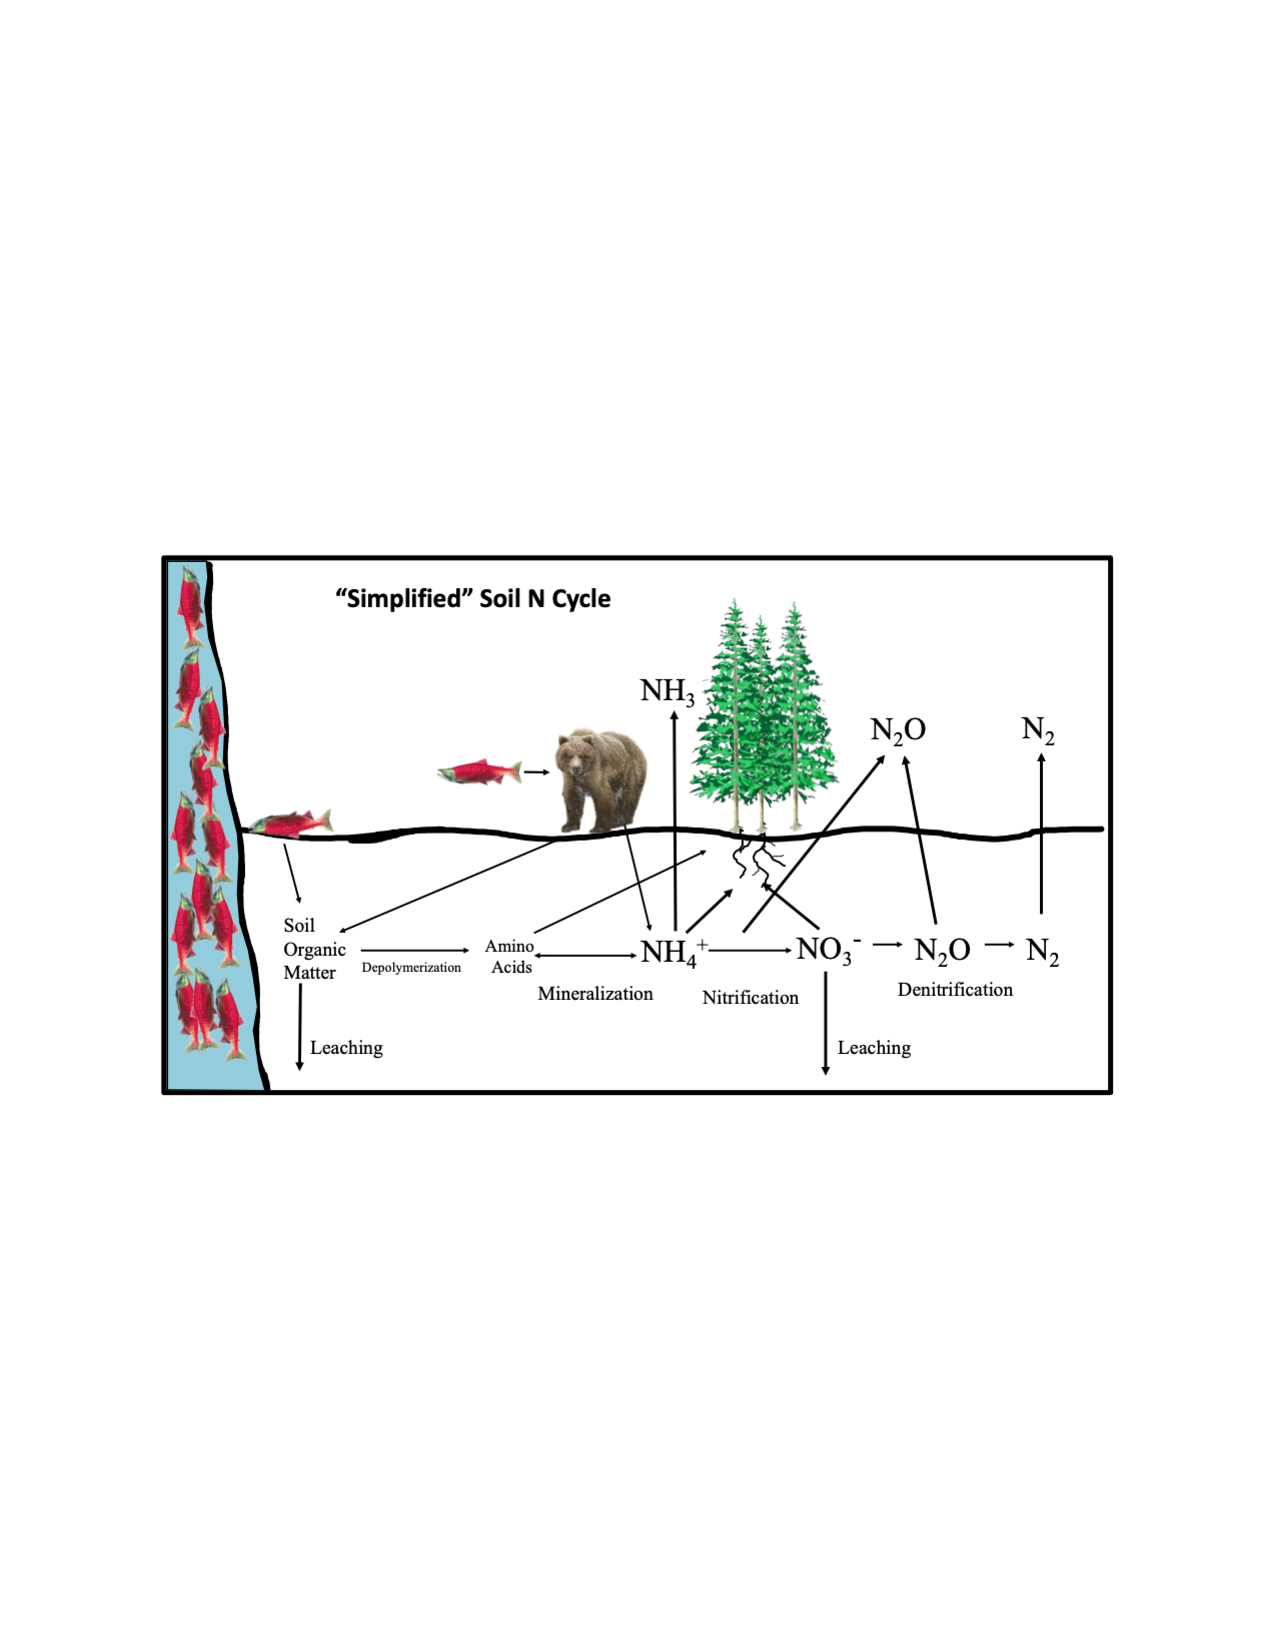
\includegraphics{figure/Ch1/fig1.1.pdf}
  \caption{Nitrogen pathways in soil}
  \label{fig:npathways}
\end{figure}
\clearpage

\textbf{Figure} \ref{fig:modIsotope}: Data (closed circles) and
predicted values (open circles) for the model with the most support
(Table \ref{tab:suppmod1}) for soil organic \(\delta^{15}N\) and
\(\delta^{13}C\), \(\delta^{15}N\) of
NH\textsubscript{4}\textsuperscript{+}, and C:N for both the
salmon-enhanced and the salmondepleted banks of Hansen Creek at 1, 3, 6,
10, and 20 m from the edge of the creek bed with 95\% confidence
intervals (dashed line) for predicted values. Blue (a and c) denotes
measures of marine-derived nitrogen, and green (b and d) denotes site
variable factors.\newline
\begin{figure}[h]
  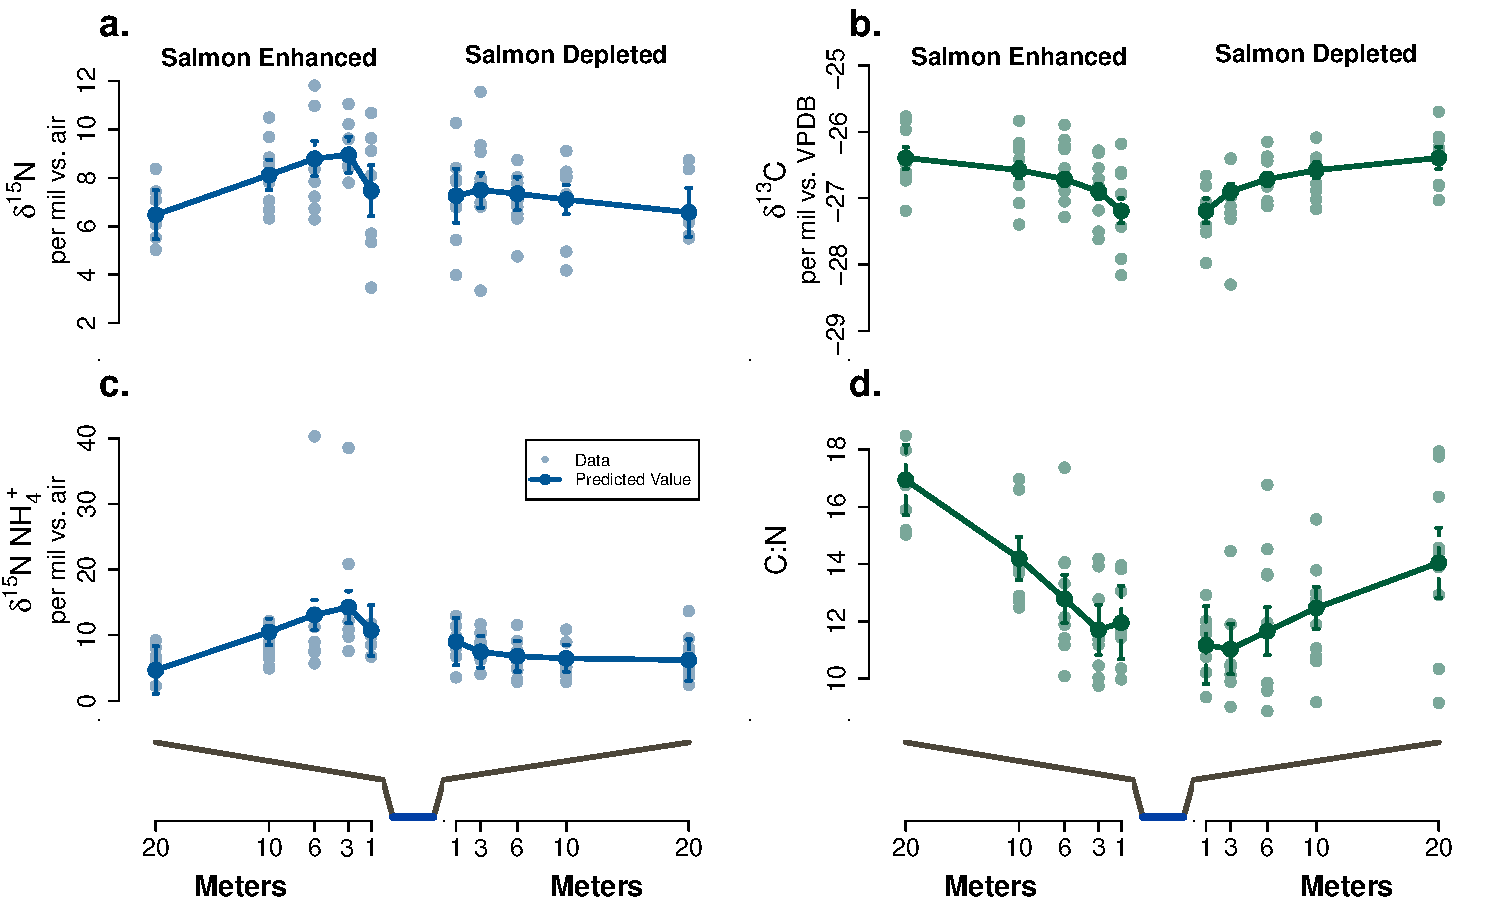
\includegraphics[width=0.85\textwidth]{figure/Ch1/Figure2_Feddernetal.pdf}
  \caption{Data and predicted values for the model with the most support: Stable Isotopes}
  \label{fig:modIsotope}
\end{figure}
\clearpage

\textbf{Figure} \ref{fig:modConc}: Data (closed circles) and predicted
values (open circles) for the model with the most support (Table
\ref{tab:suppmod1}) for NH\textsubscript{4}\textsuperscript{+} and
NO\textsubscript{3}\textsuperscript{-}, net mineralization and
nitrification, {[}N\textsubscript{org}{]}, and gravimetric water content
for both the salmon-enhanced and the salmon-depleted banks of Hansen
Creek at 1, 3, 6, 10, and 20 m from the edge of the creek bed with 95\%
confidence intervals (dashed line) for predicted values. Red (a, b, c,
d) denotes measures of soil productivity, and green (e and f) denotes
site variable factors.\newline 
\begin{figure}[h]
  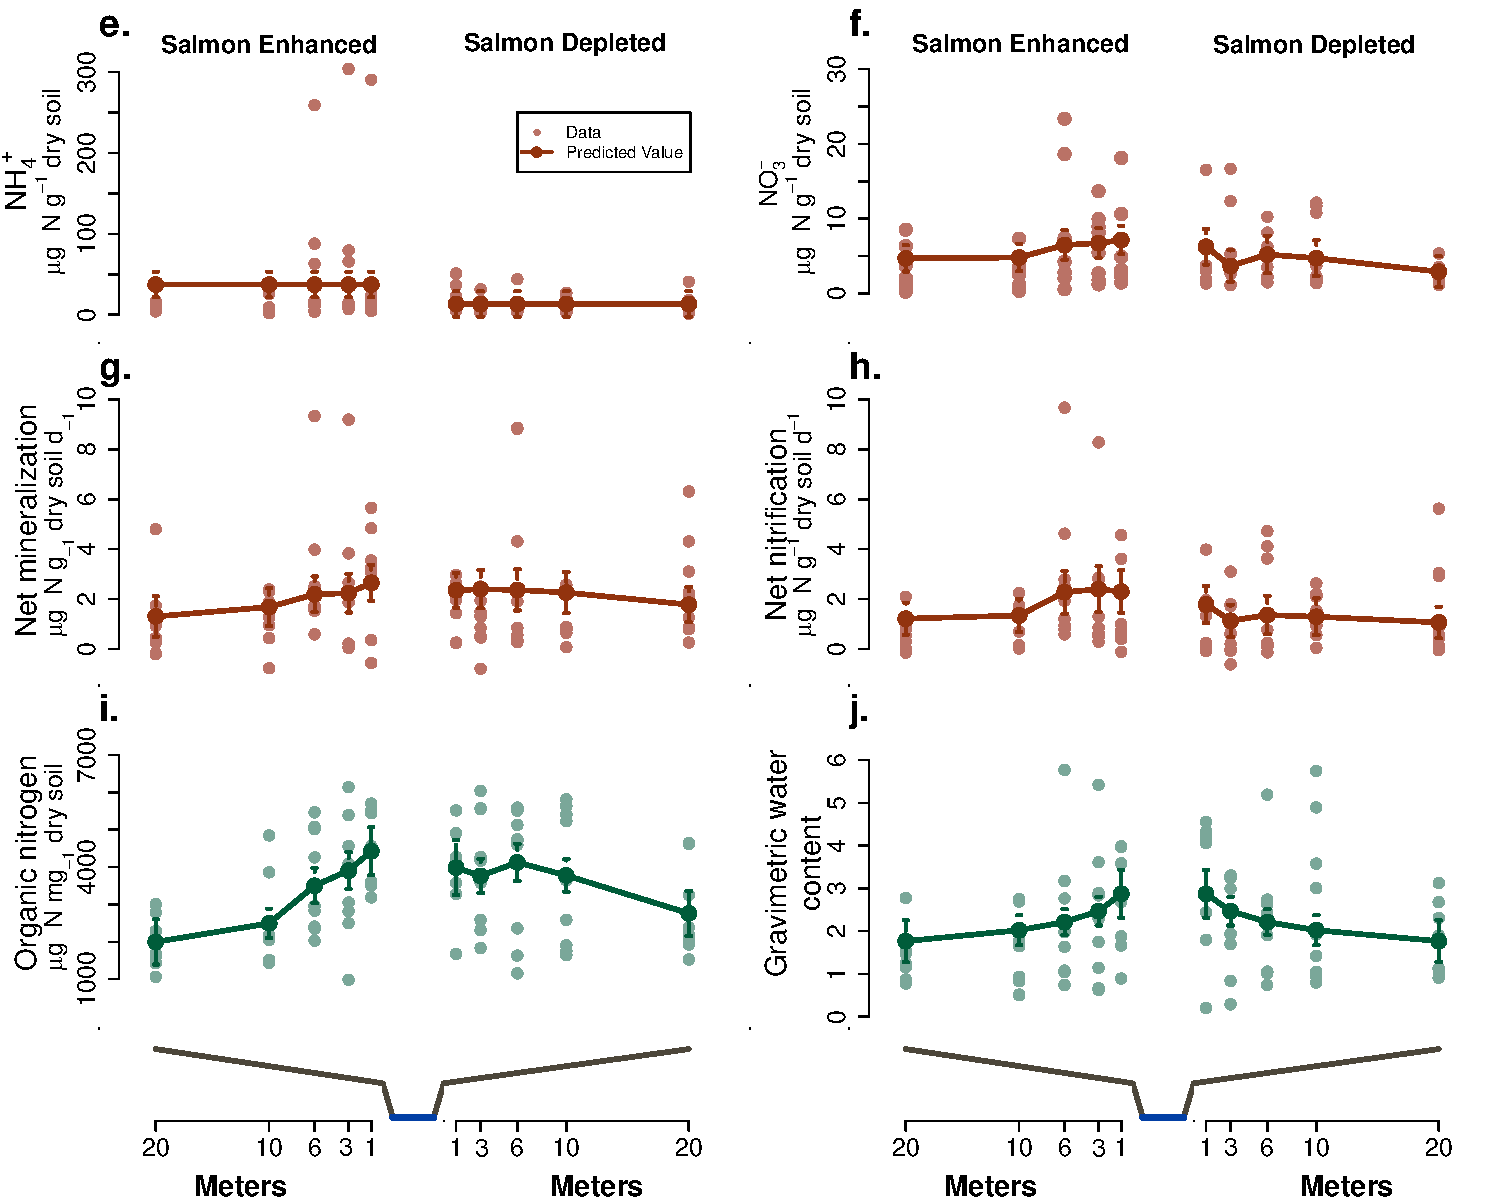
\includegraphics[width=0.85\textwidth]{figure/Ch1/Figure3_Feddernetal.pdf}
  \caption{Data and predicted values for the model with the most support: Concentrations and Transformations}
  \label{fig:modConc}
\end{figure}
\clearpage

\textbf{Figure} \ref{fig:ch1resid}: Predicted verse observed values and
predicted verse residuals for the model with the most support (Table
\ref{tab:suppmod1}, Figure \ref{fig:modIsotope}, \ref{fig:modConc}) for
each the response variables. \newline 
\begin{figure}[h]
  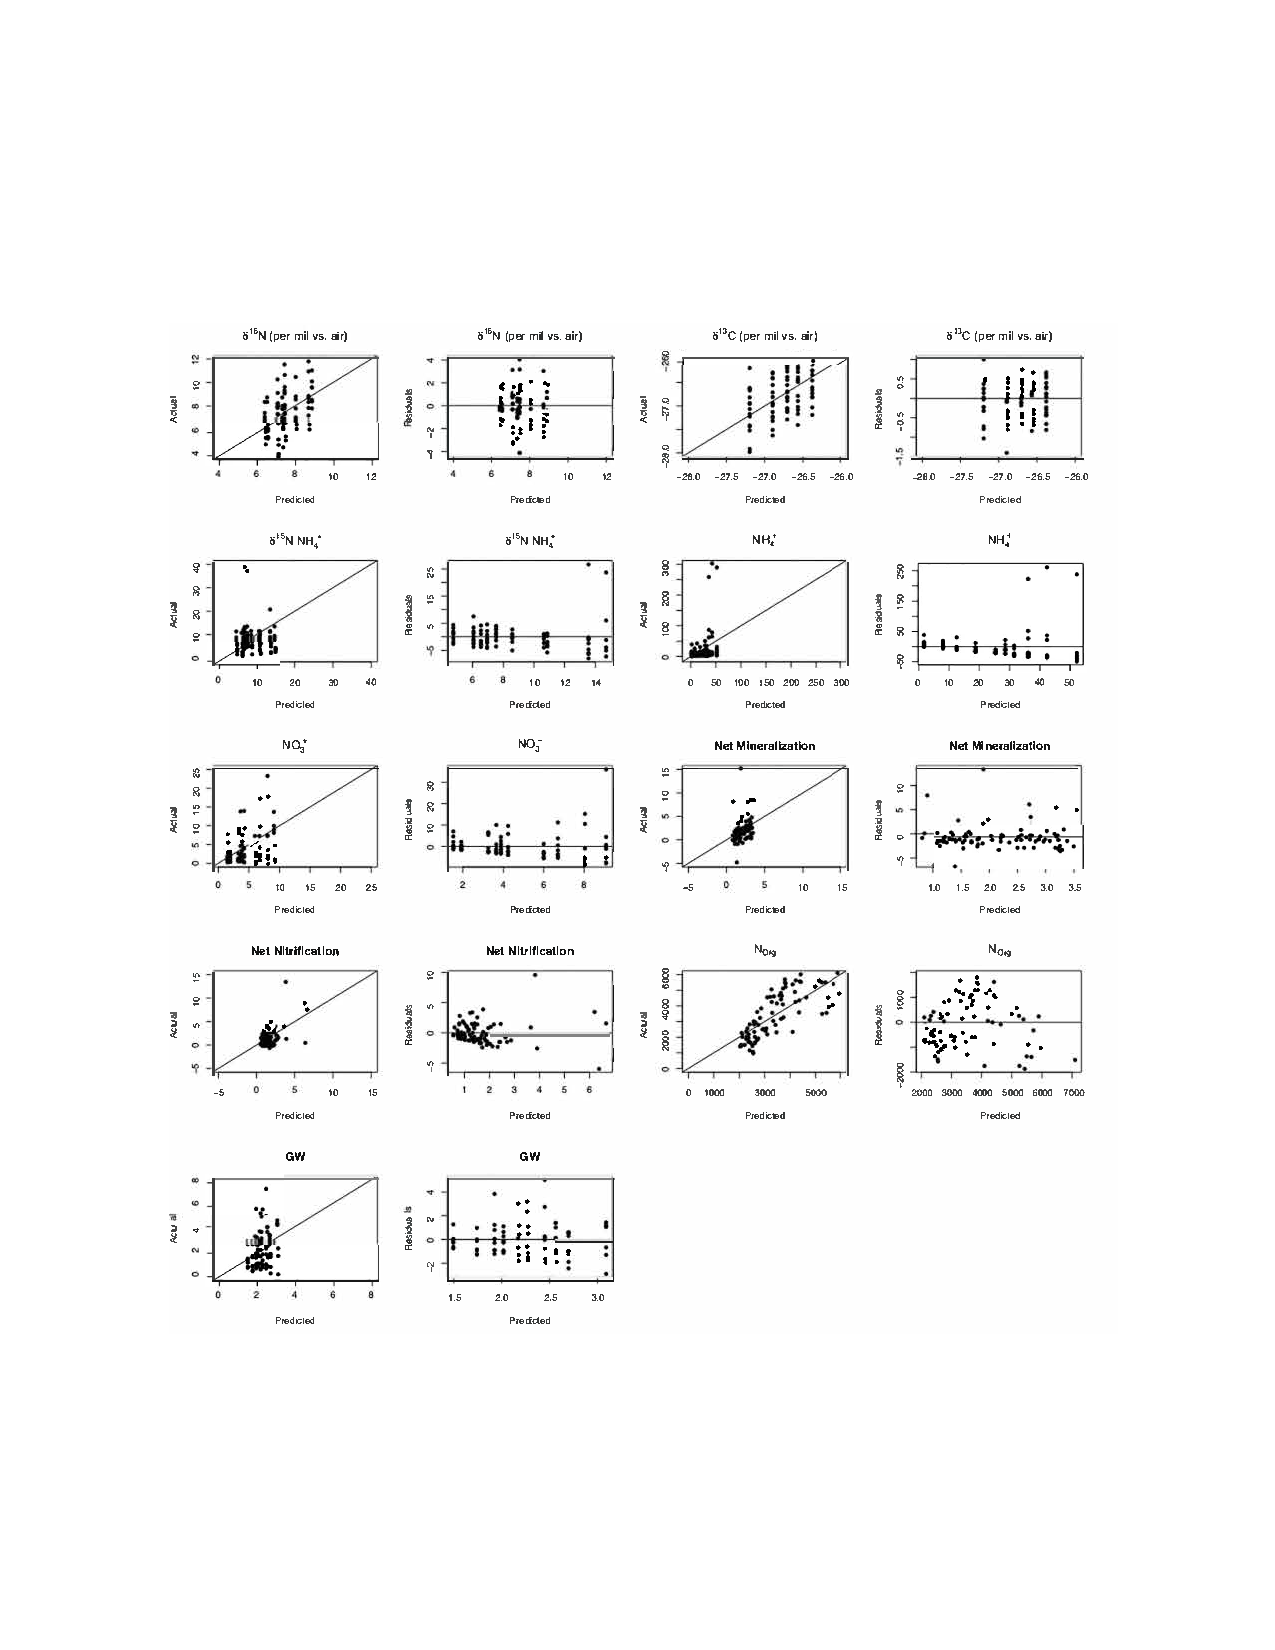
\includegraphics[width=1\textwidth]{figure/Ch1/ch1residuals.pdf}
  \caption{Residual Plots for Best Models}
  \label{fig:ch1resid}
\end{figure}
\chapter{Stable isotope signatures in historic harbor seal bone link
food web-assimilated carbon and nitrogen resources to a century of
environmental
change}\label{stable-isotope-signatures-in-historic-harbor-seal-bone-link-food-web-assimilated-carbon-and-nitrogen-resources-to-a-century-of-environmental-change}

A version of this chapter was published as: Feddern, M. L., Holtgrieve,
G.W., \& Ward, E. J. (2021). Stable isotope signatures in historic
harbor seal bone link food web‐assimilated carbon and nitrogen resources
to a century of environmental change. Global Change Biology, 11:
2328-2342. \url{https://doi.org/10.1111/gcb.15551}

\section{Abstract}\label{abstract-1}

Anthropogenic climate change will impact nutrient cycles, primary
production, and ecosystem structure in the world's oceans, although
considerable uncertainty exists regarding the magnitude and spatial
variability of these changes. Understanding how regional-scale ocean
conditions control nutrient availability and ultimately nutrient
assimilation into food webs will inform how marine resources will change
in response to climate. To evaluate how ocean conditions influence the
assimilation of nitrogen and carbon into coastal marine food webs, we
applied a novel dimension reduction analysis to a century of newly
acquired molecular isotope data derived from historic harbor seal bone
specimens. By measuring bulk \(\delta^{13}C\) and \(\delta^{15}N\)
values of source amino acids of these top predators from 1928-2014, we
derive indices of primary production and nitrogen resources that are
assimilated into food webs. We determined coastal food webs responded to
climate regimes, coastal upwelling, and freshwater discharge, yet the
strength of responses to individual drivers varied across the northeast
Pacific. Indices of primary production and nitrogen availability in the
Gulf of Alaska were dependent on regional climate indices (i.e., North
Pacific Gyre Oscillation) and upwelling. In contrast, the coastal
Washington and Salish Sea food webs were associated with local indices
of freshwater discharge. For some regions (eastern Bering Sea, northern
Gulf of Alaska) food web assimilated production was coupled with
nitrogen sources, however other regions demonstrated no
production-nitrogen coupling (Salish Sea). Temporal patterns of
environmental indices and isotopic data from Washington state varied
about the long-term mean with no directional trend. Data from the Gulf
of Alaska, however, showed below average harbor seal \(\delta^{13}C\)
values and above average ocean conditions since 1975, indicating a
change in primary production in recent decades. Altogether, these
findings demonstrate stable isotope data can provide useful indices of
nitrogen resources and phytoplankton dynamics specific to what is
assimilated by food webs.

\section{Introduction}\label{introduction-2}

Changing ocean conditions are reshaping the structure and function of
marine food webs on regional scales. Ocean temperature (Hoegh-Guldberg
\& Bruno, \protect\hyperlink{ref-Hoegh2010}{2010}), oxygen availability
(Breitburg et al., \protect\hyperlink{ref-Brietburg2018}{2018}), and
climatic regimes such as El Niño Southern Oscillation (ENSO) (Vecchi \&
Wittenberg, \protect\hyperlink{ref-Vecchi2010}{2010}) alter nutrient
availability and cycling, and thus, the ecological structure of marine
systems. Projected global redistribution of nutrients suggests net
primary production in the ocean is likely to change both spatially and
temporally. Yet, substantial uncertainty remains, with predictions
suggesting both increases and decreases in global net primary
productivity of up to 20\% by 2100 (L. Bopp et al.,
\protect\hyperlink{ref-Bopp2013}{2013}; Gregg, Conkright, Ginoux,
O'Reilly, \& Casey, \protect\hyperlink{ref-Gregg2003}{2003}; Kwiatkowski
et al., \protect\hyperlink{ref-Kwiatkowski2017}{2017}). An important
contributor to this uncertainty is regional variability in phytoplankton
response to ocean conditions and how that variability will impact other
trophic levels and dependent fisheries (Brander,
\protect\hyperlink{ref-Brander2010}{2010}; J. K. Moore et al.,
\protect\hyperlink{ref-Moore2018}{2018}). Ocean conditions (i.e., sea
surface temperature, freshwater discharge, wind, and ice cover) have
been associated with abundance and recruitment of many fish species in
the Northeast Pacific (C. J. Cunningham et al.,
\protect\hyperlink{ref-Cunningham2018}{2018}; Puerta et al.,
\protect\hyperlink{ref-Puerta2019}{2019}; Stachura et al.,
\protect\hyperlink{ref-Stachura2014}{2014}). Nonetheless, these studies
rarely include indicators of nutrient availability or primary production
linking the ecosystem response to its environment. Understanding how
regional and local scale physical drivers control nutrient availability
and ultimately nutrient assimilation into food webs will be important
for predicting the future availability of marine resources.

A strong empirical understanding of food web response to changing ocean
conditions and nutrient constraints requires time series data that span
multiple climate regimes to decouple natural variability with long-term
anthropogenic changes. Currently, quantitative methods are also limited
in their ability to scale primary production trends to ecosystem-level
responses. Stable isotope measures of \(\delta^{15}N\)
(\textsuperscript{15}N/\textsuperscript{14}N) of individual amino acids
is an emerging tool for reconstructing trends in nitrogen sources from
historic specimens (McMahon et al.,
\protect\hyperlink{ref-McMahon2019}{2019}; Owen A. Sherwood, Guilderson,
Batista, Schiff, \& McCarthy,
\protect\hyperlink{ref-Sherwood2014}{2014}; Owen A. Sherwood, Lehmann,
Schubert, Scott, \& McCarthy,
\protect\hyperlink{ref-Sherwood2011}{2011}; Whitney, Johnson, Dostie,
Luzier, \& Wanamaker, \protect\hyperlink{ref-Whitney2019}{2019}). The
\(\delta^{15}N\) signature at the base of the food web is primarily
controlled by utilization and the isotopic signatures of different
nitrogen sources, particularly urea, nitrate, and ammonium, by primary
producers (N. Ohkouchi et al.,
\protect\hyperlink{ref-Ohkouchi2017}{2017};
\protect\hyperlink{ref-Graham2010}{2009}). Measurements of bulk
\(\delta^{15}N\) values from consumers can be difficult to attribute to
changes at the base of the food web because trophic level shifts also
effect the isotopic composition of bulk nitrogen (Fry,
\protect\hyperlink{ref-Fry2006}{2006}). Amino acid specific
\(\delta^{15}N\) data addresses this challenge, as amino acids exhibit
two distinct patterns in isotopic enrichment: trophic amino acids (i.e.,
glutamic acid, alanine, proline) become enriched in \(\delta^{15}N\)
with each trophic transfer and source amino acids (i.e., phenylalanine,
lysine, methionine) show minimal change and thus are reflective of the
base of the food web (Chikaraishi et al.,
\protect\hyperlink{ref-Chikaraishi2009}{2009}; McClelland \& Montoya,
\protect\hyperlink{ref-McClelland2002}{2002}; N. Ohkouchi et al.,
\protect\hyperlink{ref-Ohkouchi2017}{2017}).

Similar to the nitrogen stable isotope composition of amino acids as a
proxy for nitrogen sources, carbon isotopic composition has emerged as a
useful tool for assessing historic changes in phytoplankton (Lorrain et
al., \protect\hyperlink{ref-Lorrain2020}{2020}; McMahon et al.,
\protect\hyperlink{ref-McMahon2019}{2019}). However, cellular growth
rates, phytoplankton community composition, the isotopic composition of
carbon in CO\textsubscript{2}, and CO\textsubscript{2} concentration all
affect the \(\delta^{13}C\)
(\textsuperscript{13}C/\textsuperscript{12}C) values of phytoplankton in
tandem (Burkhardt, Riebesell, \& Zondervan,
\protect\hyperlink{ref-Burkhardt1999}{1999}; Lorrain et al.,
\protect\hyperlink{ref-Lorrain2020}{2020}). The relative effects of
these factors remain difficult to discern from carbon isotope data
alone. Nonetheless, carbon stable isotope data is highly correlated with
copepod biomass in the northeast Pacific and thus can be a useful
combined index of ocean productivity (Espinasse, Hunt, Batten, Pakhomov,
\& Tittensor, \protect\hyperlink{ref-Espinasse2020}{2020}). While both
source amino acid \(\delta^{15}N\) and bulk \(\delta^{13}C\) values can
be influenced by a number of biogeochemical and physiological processes
(Figure 2.1), they are useful indicators of nitrogen utilization (source
amino acid \(\delta^{15}N\)) and phytoplankton dynamics (bulk
\(\delta^{13}C\)), despite the difficulty in identifying specific
mechanisms of fractionation.

Here we use source amino acid \(\delta^{15}N\) and bulk \(\delta^{13}C\)
values of consumer bone collagen as indicators of change in food
web-assimilated nitrogen (nitrogen utilization and isotopic composition
at the base of the food web) and food web-assimilated production
(phytoplankton composition, {[}CO\textsubscript{2}{]}, cellular growth,
and physiology). These definitions assume major changes in nitrogen
utilization and phytoplankton dynamics are recorded in the stable
isotope composition of nitrogen and carbon in phytoplankton (McMahon et
al., \protect\hyperlink{ref-McMahon2019}{2019}; N. Ohkouchi et al.,
\protect\hyperlink{ref-Ohkouchi2017}{2017}; Owen A. Sherwood et al.,
\protect\hyperlink{ref-Sherwood2011}{2011}; Vega et al.,
\protect\hyperlink{ref-delaVega2021}{2021}), scaled to the spatial and
temporal resource use of consumers, and conserved with minimal trophic
fractionation (Chikaraishi et al.,
\protect\hyperlink{ref-Chikaraishi2009}{2009}). Bulk \(\delta^{13}C\)
and \(\delta^{15}N\) values of source amino acids such as phenylalanine
(\(\delta^{15}N_{Phe}\)) from long-lived, generalist consumers provide
ecosystem-level information of carbon and nitrogen dynamics that are
integrated over space, time, and multiple energy pathways in the food
web (K. S. McCann, Rasmussen, \& Umbanhowar,
\protect\hyperlink{ref-McCann2005}{2005}; Vega et al.,
\protect\hyperlink{ref-delaVega2021}{2021}). As a result, these data
sources are more relevant to questions of food web responses to
large-scale environmental forcing than discrete measurements of
inorganic nutrients or phytoplankton. Ultimately these data can be used
to understand how ecosystems have responded to environmental variability
in the past and glean insights into food web responses to oceanic
conditions in the future.

Harbor seals (\emph{Phoca vitulina}) are a particularly well-suited
predator to understand food web shifts through time because of their
primarily piscivorous diet, generalist foraging strategies, high site
fidelity, and frequent occurrence in museum specimen collections. Adult
harbor seals typically forage 5 - 10 km from haul out sites and at
depths \textless{} 200 m and are opportunistic feeders (M. M. Lance,
Chang, Jeffries, Pearson, \& Acevedo-Gutierrez,
\protect\hyperlink{ref-Lance2012}{2012}). Therefore, the nitrogen and
carbon stable isotope composition of harbor seals offer a robust
representation of the isotopic composition of carbon and nitrogen
assimilated into coastal food webs. Harbor seal specific trophic
enrichment factors for nitrogen have been quantified in controlled
feeding studies, confirming minimal trophic enrichment for phenylalanine
between seals and their prey (Germain, Koch, Harvey, \& McCarthy,
\protect\hyperlink{ref-Germain2013}{2013}). Environmentally induced
shifts in foraging patterns, specifically nearshore verse offshore
feeding, has the potential to affect the carbon isotope composition in
harbor seal tissues (Figure 2.1). We assume these behavioral effects are
minimal on annual time scales compared to changes in the carbon and
nitrogen isotope composition at the base of the food web given their
restricted foraging ranges.

We aim to identify how archived \(\delta^{15}N_{Phe}\) and bulk
\(\delta^{13}C\) values vary regionally across the northeast Pacific on
ecologically relevant scales (integrated annually and regionally) and
through time using museum harbor seal specimens from 1928-2014 (Figure
\ref{fig:map}). Additionally, we characterize abiotic factors that
influence harbor seal \(\delta^{15}N_{Phe}\) and bulk \(\delta^{13}C\)
values to identify ocean conditions important for food web assimilation
of nitrogen and carbon. The effect of regional ocean condition on the
stable isotope signature of source amino acids limits the application of
short-term datasets for productivity studies, as short-term
environmental perturbations are difficult to decouple from longer term
trends such as climate regimes (Vokhshoori \& McCarthy,
\protect\hyperlink{ref-Vokshoori2014}{2014}). We therefore identify
long-term environmental drivers that are important for interpreting
reconstructed isotope data.

\section{Methods}\label{methods-1}

\subsection{Sample Collection and
Analysis}\label{sample-collection-and-analysis}

Harbor seal bone samples were obtained from specimens curated at the
Burke Museum (University of Washington), the Slater Museum (University
of Puget Sound), the Museum of the North (University of Alaska
Fairbanks), the Royal British Columbia Museum, the Smithsonian
Institute, and the National Marine Mammal Laboratory (NOAA). Specimens
were either treated by maceration in warm water or cleaned by beetles
and soaked in a dilute ammonia solution then stored in acid free boxes.
Adult specimens were sampled from three regions: eastern Bering Sea, the
Gulf of Alaska, and Washington state, which also included 18 specimens
from the southern British Columbia coast (Figure \ref{fig:map}). We
further stratified samples from the Gulf of Alaska into two subregions
(northern and southeast) and Washington state into two subregions
(coastal and Salish Sea) for a total of five subregions. Sampling
prioritized long-term temporal coverage, specifically focusing on
climate regimes shifts (i.e., PDO). Additionally, samples with sex and
size metadata were prioritized, although it was not available for most
specimens. Metadata was accessed through
\href{http://www.vertnet.org/index.html}{VertNet} using catalogue
numbers and institution codes.

Bone samples were decalcified with the resulting collagen acid
hydrolyzed, derivatized, and analyzed for compound-specific nitrogen
stable isotope analysis (CSIA) of 11 individual amino acids, including
one source amino acid, phenylalanine (phe). Of the 11 amino acids,
phenylalanine was the only discernable source amino acid and
phenylalanine is the only amino acid data are reported in this
manuscript (Appendix S1). CSIA samples were analyzed by GC-C-irMS at the
University of Washington Facility for Compound-Specific Stable Isotope
Analysis of Environmental Samples using a Thermo Scientific Trace GC +
GC IsoLink coupled to a Delta V irMS following the procedures developed
by Y. Chikaraishi, Kashiyama, Ogawa, Kitazato, \& Ohkouchi
(\protect\hyperlink{ref-Chikaraishi2007}{2007}) and protocols by Rachel
Jeffrey's lab at University of Liverpool UK (full analytical details are
provided in Appendix 1). Individual collagen samples were analyzed in
triplicate along with a mixed amino acid standard of known isotopic
composition (Sigma-Aldrich Co.) (mean precision of analytical standard
for phenylalanine = 0.3‰). Internal and external standards were used and
data processing included a drift correction. A total of 215 specimens
were sampled from the time period of 1928-2014 for CSIA, making this the
largest CSIA dataset of a mammal to date. Decalcified collagen of 190
specimens was analyzed for bulk
\textsuperscript{13}C/\textsuperscript{12}C and bulk
\textsuperscript{15}N/\textsuperscript{14}N at the University of
Washington's IsoLab using a Costech ElementalAnalyzer, ConFlo III,
MAT253 for continuous flow-based measurements.
\textsuperscript{15}N/\textsuperscript{14}N and
\textsuperscript{13}C/\textsuperscript{12}C are reported in standard
delta notation:
\begin{equation} 
  \delta^{15}N_ ( \textperthousand vs. air) =   
  [(\frac{^{15}N/^{14}N_{Sample}}{^{15}N/^{14}N_{Air}} -1)*1000]
  \label{eq:deltN}
\end{equation}
\begin{equation} 
  \delta^{13}C_ ( \textperthousand vs. VPBD) =   
  [(\frac{^{13}C/^{13}C_{Sample}}{^{13}C/^{13}C_{VPBD}} -1)*1000]
  \label{eq:deltC}
\end{equation}
Internal laboratory standards (Bristol Bay salmon and glutamic acid)
were interspersed with samples for a two-point calibration and blank
correction (mean standard precision 0.09‰ for \(\delta^{15}N\) and 0.04‰
for \(\delta^{13}C\)). A linear drift correction was also applied using
IsoDat software. The collagen C:N ratio was used to verify the integrity
of collagen for stable isotope analysis following specimen treatment and
storage (Klinken, \protect\hyperlink{ref-vanKlinken1999}{1999}).

The isotopic composition of marine dissolved organic carbon has been
steadily depleted in \textsuperscript{13}C over the past 100 years due
to increases in anthropogenic CO\_2 in the atmosphere (referred to as
the Oceanic Seuss Effect) (P. D. Quay, Tilbrook, \& Wong,
\protect\hyperlink{ref-Quay1992}{1992}). \(\delta^{13}C\) data were
therefore corrected for the Seuss Effect using the following equation
(Misarti, Finney, Maschner, \& Wooller,
\protect\hyperlink{ref-Misarti2009}{2009}):
\begin{equation} 
 \mbox {Seuss Effect Correction Factor} =   
  d * e^{0.027*(t-1850)}
  \label{eq:seuss}
\end{equation}
Where \emph{d} is the maximum annual rate of \(\delta^{13}C\) decrease
specific to the North Pacific (-0.014 derived from P. D. Quay et al.
(\protect\hyperlink{ref-Quay1992}{1992})), \emph{t} is the year
represented by the year of specimen collection with a one-year lag. The
Seuss effect varies regionally (Tagliabue \& Bopp,
\protect\hyperlink{ref-Tagliabue2008}{2008}) and we applied a northeast
Pacific parameterization (Misarti et al.,
\protect\hyperlink{ref-Misarti2009}{2009}).

Standard linear models were used to identify whether size (standard
length, cm), sex, and subregion of the harbor seals sampled were related
to isotopic composition and to test whether these parameters needed to
be standardized in environmental models. \(\delta^{15}N_{Phe}\) and
\(\delta^{13}C\) values were modelled independently as univariate
continuous response variables using the following equation:
\begin{equation} 
 y_i \sim N(\boldsymbol{\alpha} + \boldsymbol{\beta X}_i, \sigma^2_y)
  \label{eq:linmods}
\end{equation}
where \emph{y} is the mean triplicate value for each individual \emph{i}
for either \(\delta^{15}N_{Phe}\) or \(\delta^{13}C\) values. \textbf{X}
represents the matrix of predictors (sex, length, subregion),
\(\boldsymbol{\alpha}\) is a scalar and \(\boldsymbol{\beta}\) is a
vector of coefficients for the predictors. Length (n = 116) was modelled
as a continuous variable and was natural log transformed; subregion and
sex (n = 190) were modelled as factors. Individual models were used to
test whether a predictor was significant as opposed to a multivariate
framework because, 1) sample sizes for \(\delta^{15}N_{Phe}\) (n = 215)
and \(\delta^{13}C\) (n = 190) data varied, and 2) predictor metadata
was incomplete for specimens. A pairwise t-test using the Bonferroni
correction and non-pooled standard deviation was also used to compare
differences in mean isotope signature between subregions and sex (Figure
\ref{fig:dist}, Tables \ref{tab:ttestN} \& \ref{tab:ttestC}).

To understand the extent of coupling between indices of food web
assimilated production and nitrogen resources, a linear model
representing the basin wide relationship was fit to
\(\delta^{15}N_{Phe}\) and \(\delta^{13}C\) values as continuous
variables assuming normal errors. To understand spatial variation in
this relationship, a hierarchical model was fit to the same dataset with
varying slope and varying intercept based on subregion as a random
effect. This model took the following form:
\begin{equation} 
 y_i \sim N(\boldsymbol{\alpha}_{j[i]} + \boldsymbol{\beta}_{j[i]}\boldsymbol{x}_i, \sigma^2_y)
  \label{eq:hiermods}
\end{equation}
Where \emph{y} represents \(\delta^{13}C\) values as a continuous
variable and x represents \(\delta^{15}N_{Phe}\) values as a continuous
variable and j represents the group level predictor, subregion.
\(\boldsymbol{\alpha}\) and \(\boldsymbol{\beta}\) are each vectors of
coefficients that vary by subregion.

\subsection{Quantifying effects of ocean condition on food web isotope
indices}\label{quantifying-effects-of-ocean-condition-on-food-web-isotope-indices}

Linear models were used to identify environmental drivers of
\(\delta^{13}C\) and \(\delta^{15}N_{Phe}\) values using a suite of
environmental indices as covariates. A total of 42 environmental time
series were compiled as potential predictor variables (Table 2.2) based
on previous evidence for food web importance in the northeast Pacific
(Di Lorenzo et al., \protect\hyperlink{ref-DiLorenzo2008}{2008};
Stachura et al., \protect\hyperlink{ref-Stachura2014}{2014}). Each
environmental time series was standardized around a mean of 0 and
standard deviation of 1 and discharge data was also natural log
transformed. We divided these environmental covariates a priori into
four main mechanistic properties based on the expected effect on
nutrient assimilation into the food web: climate regime, freshwater
discharge, circulation (wind and upwelling), and sea surface temperature
(Figure 2.1). Given the three regions in our analysis, each of these
hypotheses were also divided according to our regional geographic breaks
(eastern Bering Sea, Gulf of Alaska, and Washington). To reduce
collinearity between environmental time series and reduce the total
number of candidate models, a subset of 7 environmental times series
were selected for each region based on the temporal overlap with stable
isotope data. Each subset contained at least one time series for each of
the four mechanistic properties and all possible combinations of
predictors were tested (Table 2.3). While reduction of the number of
times series provides analytical benefits, it comes at the cost of
potentially conservative estimates of which covariates are important,
meaning important components of ocean condition to the food webs may be
missed.

\(\delta^{15}N_{Phe}\) and \(\delta^{13}C\) values were independently
considered as response variables to evaluate relationships between
predictors (environmental indices and location) and stable isotope data
using Figure \eqref{eq:linmods} where X is a matrix of predictors using
the 7 standardized environmental time series (continuous) and subregion
(factor) as covariates. We treated carbon and nitrogen isotopes as
response variables separately in linear models, rather than in a
combined multivariate model due to differences in sample size and
differences in the strength of correlation between for
\(\delta^{15}N_{Phe}\) and \(\delta^{13}C\) values for each subregion.
Time series data prior to 1950 and after 2014 was excluded from this
analysis as data for some covariates did not extend beyond 1950.
Candidate models (n = 53) were compared using Akaike Information
Criteria with a small sample size correction {[}AICc{]} and included all
combinations of the environmental indices. In addition, a subregion
factor was included with two levels for Washington (Salish Sea and
coastal Washington) and the Gulf of Alaska (southcentral and southeast)
and a null model (intercept only) was also tested. Tissue turnover time
of bone collagen has not been measured in mammals of this size to our
knowledge but is approximately 173 days for birds (K. A. Hobson \&
Clark, \protect\hyperlink{ref-Hobson1992}{1992}). Thus, a lag of one
year was applied to the stable isotope datasets to account for the
timing of tissue turnover in bone collagen. To validate this approach of
applying a 1-year lag, 0- and 2-year lags were also applied to the best
models of each region an compared to the 1-year lag using AIC.
Additionally, month was tested as a smoothed predictor with 12 knots for
stable isotope data in Washington samples using a generalized additive
model (GAM). Support for a significant smoothing term would identify and
seasonality in the data, which would be expected if tissue turnover time
is less than a year. A one-year tissue turnover time was confirmed as a
suitable assumption for harbor seal bone collagen, as 0- and 2- year
lags had similar or less model support. There was no support for a
smoothing effect by month in generalized additive models of
\(\delta^{15}N_{Phe}\) and \(\delta^{13}C\) which would have indicated
any seasonal variability in isotope composition and thus a turnover time
of less than or greater than a year (p \textless{} 0.05; Figure
\ref{fig:Length}) and thus a 1-year lag was applied to isotope data for
all temporal analyses.

For each model with relatively high support (ΔAICc \textless{} 2) the
AICc weight and the coefficient for each covariate is reported (Figure
\ref{fig:dist}. To confirm collinearity was not problematic in the
candidate models that included more than one environmental covariate,
matrix scatterplots and variance inflation factors (vif) were used from
the car package (Fox et al. 2019) in R (R Development Core Team, 2020).

\subsection{Gaussian Process Dynamic Factor Analysis
(GPDFA)}\label{gaussian-process-dynamic-factor-analysis-gpdfa}

To further understand how the environment, \(\delta^{13}C\), and
\(\delta^{15}N_{Phe}\) values covary through time in the Northeast
Pacific, we developed a novel extension of conventional Dynamic Factor
Analysis (DFA). DFA is a dimension reduction technique that identifies
common processes underlying a set of multivariate time series. This
technique has been applied to multivariate time series problems in
fisheries and ecology to identify patterns of oceanographic variability
that drive Pacific salmon stocks (Jorgensen, Ward, Scheuerell, \& Zabel,
\protect\hyperlink{ref-Jorgensen2016}{2016}; Ohlberger, Scheuerell,
Schindler, \& Peters, \protect\hyperlink{ref-Ohlberger2016}{2016};
Stachura et al., \protect\hyperlink{ref-Stachura2014}{2014}).

DFA models identify common trends across multiple time series (``latent
trends'') and estimates the importance of that trend for each individual
time series as a coefficient (``factor loading''). The two equations
describing DFA take on the following form:
\begin{equation} 
 \boldsymbol{y}_t = \boldsymbol{Zx}_t + \boldsymbol{v}_t,\mbox{ where }\boldsymbol{v}_t \sim MVN(0,\boldsymbol{R})
  \label{eq:gdfa1}
\end{equation}
\begin{equation} 
 \boldsymbol{x}_t = \boldsymbol{x}_{t-1} + \boldsymbol{w}_t,\mbox{ where }\boldsymbol{w}_t \sim MVN(0,\boldsymbol{I})
  \label{eq:gdfa2}
\end{equation}
The observed data \textbf{y}\textsubscript{t} are modeled as
combinations of latent trends \textbf{x}\textsubscript{t} at time
\emph{t} (the dimensions of \textbf{x}\textsubscript{t} matching the
number of trends which are also referred to as states) and factor
loadings (\textbf{Z}) (a coefficient for each time series for each
trend) at time \emph{t}, which are modeled as a random walk (Zuur et al.
2003). In addition there is an optional random observation error
(\textbf{v}\textsubscript{t}) and process error
(\textbf{w}\textsubscript{t}) which are multivariate normal

Our extension of DFA adopts an alternative model of the latent trends,
modeling them with Gaussian Processes rather than random walks.Gaussian
Processes (GP) have been widely used in fisheries and other fields (S.
B. Munch, Giron‐Nava, \& Sugihara,
\protect\hyperlink{ref-Munch2018}{2018}). Instead of modeling a time
series as an autoregressive process, GPs model a time series via a mean
and variance function, \emph{x\textasciitilde{}}\(MVN(u,\Sigma)\) where
\emph{u} represents and optional mean vector and \textbf{Σ} a covariance
matrix. For GPDFA, we assume the mean to be zero, letting just the
covariance function determine the GP smoothing. GPs are flexible in that
the covariance matrix can be described by a wide range of flexible
functions; for this application we use a Gaussian kernel (squared
exponential) so that \(\Sigma_{i,j}=\sigma^2 exp(-d_{i,j}/\sigma)\),
where \(\sigma^2\) is a variance parameter controlling the magnitude, θ
is a shape parameter controlling how quickly covariance declines, and
\(d_{i,j}\) is the known distance between time points \emph{i} and
\emph{j}. A benefit of modeling \textbf{Σ} with a covariance function is
that regardless of the dimensionality, all elements of \textbf{Σ} can be
described by a small number of parameters. For GPDFA, we choose to use a
GP predictive process model, because the number of time points may be
large (Latimer, Banerjee, Sang Jr, Mosher, \& Silander Jr,
\protect\hyperlink{ref-Latimer2009}{2009}). This predictive model
estimates the function values at a subset of locations (knots), and
combines these estimates with the distance to locations at which data
are observed to make predictions. More specifically, the values of the
time series at the knot locations are
\(x^*\)\textasciitilde{}\(MVN(0,\Sigma^*)\). Given the known distances
between the locations of knots and locations of data, the covariance
matrix between the two can be calculated, \(\Sigma_{(x,x^*)}\). Finally,
the predictions of the time series at the observed data can be
calculated as \(\hat{x}=\Sigma'_{(x,x^*)}\Sigma^{*-1}x^*\). In this
extension of DFA, all other model components are identical to the
conventional time series version with latent trends modeled as a random
walk.

With the Gaussian Process DFA model, a decision needs to be made a
priori about selecting the number and location of knots, where the
function parameters are estimated at. There are multiple approaches for
doing this; we adopted a model with 15 knots (more knots resulting in a
smoother function), and estimated the knot location by performing a
clustering approach of the years corresponding to the raw observations
(partitioning around medoids, using the `pamk' function in the fpc
library in R).

With conventional DFA using an autoregressive model, long gaps in time
series data result in large, overestimations of the variance of the
latent trends. Gaussian Processes model time series as a multivariate
normal distribution, with estimated mean vector \textbf{u} and
covariance matrix \textbf{Σ} (S. B. Munch et al.,
\protect\hyperlink{ref-Munch2018}{2018}). To constrain the number of
estimated parameters, elements of \textbf{Σ} were modeled with a
Gaussian or squared covariance exponential function such that
\(\Sigma_{(i,j)}= \sigma^2 exp(-(t_i-t_j )^2/\theta)\). In this
parameterization, \(\sigma^2\) controls the variability of the
stochastic process, \(\theta\) controls the rate of decay in correlation
between time steps, and t\textsubscript{i} and t\textsubscript{j} are
the time variables (e.g.~years) for locations \emph{i} and \emph{j}.

We considered models with 1- 4 underlying trends. Each trend was
modelled separately (different means) but models with multiple trends to
have a shared covariance matrix amongst trends. The GPDFA approach was
applied to time series from each region and the best model was selected
using leave-one-out cross-validation (LOOIC) from the loo package in R
(Vehtari, Gelman, \& Gabry, \protect\hyperlink{ref-Vehtari2017}{2017}).
The choice of knots affects the degree of smoothness, with more knots
creating more smooth functions. We tested several different numbers of
knots and found results to be qualitatively similar. Similar to the
previous analysis, time series data prior to 1948 for Washington state
and prior to 1940 and after 2008 for the Gulf of Alaska was excluded
from this analysis. We fit GPDFA to data from each region including all
of the initial 42 identified environmental time series for that region
(Table 2.2), \(\delta^{15}N_{Phe}\) and \(\delta^{13}C\) values, with
location as a factor. We implemented GPDFA using the Stan language (Stan
Development Team 2019, B. Carpenter et al.,
\protect\hyperlink{ref-Carpenter2017}{2017}), and R (R Core Development
Team 2019, version 3.6.2) via R package rstan (Stan Development Team
2019, version 2.21.2). Code to implement GPDFA is available
\href{https://github.com/mfeddern/CSIA-AA/blob/master/SourceData/Src/Analysis/gpdfa.stan}{here}

\section{Results}\label{results-1}

\(\delta^{15}N_{Phe}\) and bulk \(\delta^{13}C\) values did not vary by
sex (p \textgreater{} 0.05, Figure \ref{fig:dist} or size for the
individuals sampled (p \textgreater{} 0 .05; Figure \ref{fig:Length}).
Spatial variation in harbor seal \(\delta^{15}N_{Phe}\) and
\(\delta^{13}C\) values were observed on subregional scales.
\(\delta^{15}N_{Phe}\) values were similar for harbor seals in the
northern Gulf of Alaska (11.9 ± 2.9, mean ± 1SD), southeast Gulf of
Alaska (10.8 ± 1.7), and coastal Washington (11.3 ± 1.9). The eastern
Bering Sea had significantly higher \(\delta^{15}N_{Phe}\) values
compared to other subregions (15.2 ± 1.8) followed by the Salish Sea
(12.2 ± 2.3) which had similar \(\delta^{15}N_{Phe}\) values compared to
the northern Gulf of Alaska (Figure \ref{fig:dist}, Table
\ref{tab:ttestN}). \(\delta^{13}C\) values varied by subregion (p
\textless{} 0.05) with the exception of the Gulf of Alaska, where the
northern (-14.6 ± 0.9) and southeast (-14.4 ± 1.1) subregions were not
significantly different, and the eastern Bering Sea (-13.4 ± 0.9) and
coastal Washington (-13.6 ± 0.9) were not significantly different
(Figure \ref{fig:dist}, Table \ref{tab:ttestC}). The variation between
subregions appeared to follow a latitudinal gradient, where harbor seal
mean \(\delta^{13}C\) values were most enriched in \(^{13}C\) in the
Salish Sea (-12.2 ± 1.5), became more depleted from coastal Washington
and into the Gulf of Alaska (Table \ref{tab:ranges}).

The relationship between harbor seal \(\delta^{15}N_{Phe}\) and
\(\delta^{13}C\) values also varied on subregional scales. There was
positive linear association between harbor seal \(\delta^{15}N_{Phe}\)
and \(\delta^{13}C\) values in the combined northeast Pacific basin and
Bering Sea model with a slope of 0.12 (Figure \ref{fig:hiermod}A). For
the hierarchical subregion model, the eastern Bering Sea and coastal
Washington demonstrated similar relationship, with slopes of 0.08 (95\%
CI {[}0.05, 0.11{]}) and 0.07 (95\% CI {[}0.05, 0.09{]}) respectively.
Similarly, harbor seals in both Gulf of Alaska subregions demonstrated
comparable coupling of \(\delta^{15}N_{Phe}\) and \(\delta^{13}C\), with
slopes of 0.13 (95\% CI {[}0.11, 0.14{]}) for the northern subregion and
0.12 (95\% CI {[}0.10, 0.14{]}) for the southeastern subregion. Salish
Sea harbor seals had a distinct relationship between
\(\delta^{15}N_{Phe}\) and \(\delta^{13}C\) values relative to other
subregions with a slope of only 0.02 that was not significantly
different from 0 (95\% CI {[}0.0, 0.04{]}) (Figure \ref{fig:hiermod}B).

For both \(\delta^{15}N_{Phe}\) and \(\delta^{13}C\) values there was
substantial support for models including environmental indices rather
than null or subregion only models. The relationship between
environmental indices and harbor seal \(\delta^{15}N_{Phe}\) and
\(\delta^{13}C\) values in the northeast Pacific varied on regional
scales. For Washington, the best model to predict harbor seal
\(\delta^{15}N_{Phe}\) values included Columbia River discharge in high
flow months, summer upwelling, and subregion. There was substantial
model uncertainty for \(\delta^{15}N_{Phe}\) values in the Washington
region, however 90\% of model weight supported the inclusion of Columbia
River discharge (Figure \ref{fig:coefres}A). The model for harbor seal
\(\delta^{13}C\) values with the most support indicated a positive
association between PDO, spring upwelling, and freshwater discharge in
the Washington region (Figure \ref{fig:coefres}B). In the Gulf of
Alaska, the summer upwelling model had the most support as a predictor
of harbor seal \(\delta^{15}N_{Phe}\) values with some model support for
inclusion of the NPGO (North Pacific Gyre Oscillation), although the
coefficients for this covariate did not differ substantially from 0
(Figure \ref{fig:coefres}C). The best model for harbor seal
\(\delta^{13}C\) values for the Gulf of Alaska included subregion, PDO
(Pacific Decadal Oscillation), and NPGO (Figure \ref{fig:coefres}D). In
contrast to Washington, the Gulf of Alaska models supported a negative
association between δ13C values and PDO. The null model for
\(\delta^{15}N_{Phe}\) values in the eastern Bering Sea had the most
support (Figure \ref{fig:coefres}E). Lack of model support for
environmental covariates in the eastern Bering Sea may have been a
result of the small sample size in the region. Cross-shelf wind was
included as a predictor in the best model (Figure \ref{fig:coefres}F)
for \(\delta^{13}C\) values in the eastern Bering Sea and was supported
by 76\% of the model weight.

PDO and Kuskokwim river discharge during high flow months were found to
be highly collinear (VIF \textgreater{} 10) and PDO was omitted from the
candidate model set for the eastern Bering Sea analysis. All other
models containing multiple environmental predictors with relative
support had variance inflation factors of less than 2 indicating only
moderate collinearity across covariates. Model residuals for the best
models did not show trends through time (Figure \ref{fig:linresid}).
This indicates that there were no trends associated with other potential
ecosystem changes, such as harbor seal foraging strategy for example,
after accounting for ocean condition. Model results did not change when
using \(\delta^{13}C\) data that were not corrected for the regional
Seuss Effect.

The GPDFA analysis showed temporal synchronies and shared trends across
environmental conditions and stable isotope values in the northeast
Pacific. In the Gulf of Alaska, the data supported three latent trends
(Figure \ref{fig:GDFAAK}). Both \(\delta^{15}N_{Phe}\) and
\(\delta^{13}C\) values had the highest loadings for trend 1, which
showed an increase starting in 1965 until 1980 followed by the trend
oscillating at approximately 25\% above the long-term average. The
harbor seal \(\delta^{15}N_{Phe}\) values for the southeast subregion,
harbor seal \(\delta^{13}C\) values, and spring upwelling had negative
loadings on trend 1; loadings of \(\delta^{15}N_{Phe}\) values were
generally weaker relative to loadings of \(\delta^{13}C\) values. For
the other two trends (2-3), loadings were clustered by environmental
driver category. Latent trend 2 oscillated around the long-term average
and was uninformative. Trend 3 was below average starting in 1985 with
strong loadings for climate time series, spring and summer upwelling,
and discharge in high flow months (Figure \ref{fig:GDFAAK}). Annual
discharge, autumn upwelling, Oceanic Niño Index and Northern Oscillation
Index did not demonstrate strong loadings for any trend. In Washington,
there was support for two latent trends. Latent trend 1 shows a rapid
increase in the 1940's to 25\% above the long-term mean then a gradual
decline until 1986 to approximately 40\% below the long-term mean, with
values below the mean starting in 1977 (Figure \ref{fig:GDFAWA}). Trend
loadings for harbor seal \(\delta^{15}N_{Phe}\) and \(\delta^{13}C\)
values were stronger for coastal seals and trend 1 had stronger loadings
for freshwater discharge than trend 2. Trend 2 had strong loadings for
\(\delta^{15}N_{Phe}\) and \(\delta^{13}C\) values for both Salish Sea
and coastal Washington harbor seals. Trend 2 oscillated above and below
the long-term mean and had large loadings for sea surface temperature,
summer upwelling, Fraser River discharge and climate indices (Figure
\ref{fig:GDFAWA}).

To validate this approach of applying a 1-year lag, 0- and 2-year lags
were also applied to the best models of each region an compared to the
1-year lag using AIC. Additionally, month was tested as a smoothed
predictor with 12 knots for stable isotope data in Washington samples
using a generalized additive model (GAM). Support for a significant
smoothing term would identify and seasonality in the data, which would
be expected if tissue turnover time is less than a year. A one-year
tissue turnover time was confirmed as a suitable assumption for harbor
seal bone collagen, as 0- and 2- year lags had similar or less model
support. There was no support for a smoothing effect by month in
generalized additive models of \(\delta^{15}N_{Phe}\) and
\(\delta^{13}C\) which would have indicated any seasonal variability in
isotope composition and thus a turnover time of less than or greater
than a year (p \textless{} 0.05; Figure \ref{fig:Length}) and thus a
1-year lag was applied to isotope data for all temporal analyses.

\section{Discussion}\label{discussion-1}

We analyzed bone collagen \(\delta^{15}N_{Phe}\) and bulk
\(\delta^{13}C\) values from harbor seal museum specimens collected
between 1928 and 2014 as indices of change in food web assimilated
nitrogen and carbon. Based on previous research (Lorrain et al.,
\protect\hyperlink{ref-Lorrain2020}{2020}; Owen A. Sherwood et al.,
\protect\hyperlink{ref-Sherwood2014}{2014}; Vega, Jeffreys, Tuerena,
Ganeshram, \& Mahaffey, \protect\hyperlink{ref-delaVega2019}{2019}), we
interpret \(\delta^{15}N_{Phe}\) and bulk \(\delta^{13}C\) values as
primarily representing nitrogen and carbon resource utilization, and
growth and community composition of primary producers at the base of the
food web. Our data show the relationship between indices of primary
production and nitrogen resources assimilated into food webs varies
regionally across the northeast Pacific. By pairing these data with
environmental time series data, we provide new insights into large scale
environmental forcing that impacts the base of the food web and is
transferred to higher trophic levels. Specifically, oceanic conditions
associated with climate regimes and upwelling explain significant
temporal variation in \(\delta^{15}N_{Phe}\) and bulk \(\delta^{13}C\)
values of coastal predators in northeast Pacific (Figure
\ref{fig:coefres}; Figure \ref{fig:linresid}). This analysis
demonstrates \(\delta^{15}N_{Phe}\) and bulk \(\delta^{13}C\) values are
useful indicators of resources assimilated by coastal food webs.

\subsection{Spatial variation in stable isotope
indices}\label{spatial-variation-in-stable-isotope-indices}

The geographically widespread association between harbor seal
\(\delta^{15}N_{Phe}\) and bulk \(\delta^{13}C\) values indicates food
web assimilated primary production is coupled with nitrogen resources in
most regions of the northeast Pacific, with the Salish Sea as a notable
exception (Figure \ref{fig:hiermod}). Short-term studies in coastal
Washington showed phytoplankton respond considerably to nitrogen inputs
and are frequently nitrogen limited (Dortch \& Postel,
\protect\hyperlink{ref-Dortch1989}{1989}; R. M. Kudela \& Peterson,
\protect\hyperlink{ref-Kudela2009}{2009}). Similarly, short term studies
of the inner Gulf of Alaska shelf demonstrated primary production is
generally nitrogen limited, and size, growth rates, and community
composition are all tightly coupled with nutrient availability (S. L.
Strom, Olson, Macri, \& Mord, \protect\hyperlink{ref-Strom2006}{2006}).
A significant relationship between bulk \(\delta^{15}N\) and
\(\delta^{13}C\) values was also observed in the tissues of some
gorgonian corals over the same time period in coastal Gulf of Alaska (B.
Williams, Risk, Stone, Sinclair, \& Ghaleb,
\protect\hyperlink{ref-Williams2007}{2007}). Given the evidence of
nitrogen limitations and its relationship with phytoplankton growth and
community composition in these coastal environments, the association
between \(\delta^{15}N_{Phe}\) and bulk \(\delta^{13}C\) values could be
the result of nitrogen limiting growth at the base of the food web.
Alternatively, the \(\delta^{15}N_{Phe}\) and bulk \(\delta^{13}C\)
coupling could be driven by covariance with an untested environmental
variable that impacts most of the northeast Pacific but not the Salish
Sea.

The coastal Washington and the Salish Sea food webs assimilate different
nitrogen and carbon sources (Figure \ref{fig:coefres} A \& B). Salish
Sea harbor seals have higher \(\delta^{15}N_{Phe}\) and bulk
\(\delta^{13}C\) values compared to individuals on the outer coast,
which is likely due to significant contributions of intertidal producers
and the legacy of anthropogenic N in the Salish Sea food web. Intertidal
macrophytes (seagrass and algae) have similar δ13C values
(\textasciitilde{} -10‰) compared to harbor seals in the Salish Sea,
while other potential sources are much lower (i.e., marine derived
sources \textasciitilde{} -20‰, terrestrial derived sources
\textasciitilde{} -30‰) (Conway-Cranos et al.,
\protect\hyperlink{ref-Conway2015}{2015}; Howe \& Simenstad,
\protect\hyperlink{ref-Howe2015}{2015}). Incorporation of intertidal
producers into the Salish Sea food web explains the difference in carbon
stable isotope signatures between Salish Sea and coastal Washington
harbor seals (\textasciitilde{}1.4‰, Figure \ref{fig:coefres}A).
However, it does not explain the higher \(\delta^{15}N_{Phe}\) values
(Figure \ref{fig:coefres}B, Table \ref{tab:ranges}). Surface nitrate was
observed to be 8‰ -- 12‰ off the coast of Washington in spring 1993 (J.
Wu, Calvert, \& Wong, \protect\hyperlink{ref-Wu1997}{1997}) which was
exceeded by harbor seals in both coastal Washington and the Salish Sea
(Table \ref{tab:ranges}). It is likely anthropogenically derived
nitrogen sources contribute to the higher observed
\(\delta^{15}N_{Phe}\) values both directly and indirectly, particularly
in the Salish Sea where harbor seal \(\delta^{15}N_{Phe}\) values were
up to 2.4‰ higher than coastal Washington seals. Wastewater treatment
facilities and agriculture runoff contribute substantial amounts
(\textasciitilde{}32\%) of nitrogen in the Salish Sea (Mohamedali et al.
2011) and are enriched in \(^{15}N\). In recent decades, Salish Sea
waters have also been characterized by low dissolved oxygen and hypoxic
events (PSEMP 2019) from human derived nitrogen loading. Anoxic
conditions are conducive to denitrification, another potential indirect
source of \(^{15}N\) from human activities in the region.

\subsection{Ocean condition and stable isotope
indices}\label{ocean-condition-and-stable-isotope-indices}

Washington state food webs exhibit environmentally induced changes in
assimilated primary production and nitrogen sources. The isotope-ocean
condition relationship in the region can be explained by introduction of
terrestrial derived nutrients and climatically induced changes in
phytoplankton community structure observed in previous studies (Du \&
Peterson, \protect\hyperlink{ref-Du2014}{2014}; R. Kudela et al.,
\protect\hyperlink{ref-Kudela2008}{2008};
\protect\hyperlink{ref-Du2015}{2015}). For example, the PDO has been
associated with phytoplankton community shifts between dinoflagellates
and diatoms in the northern California Current
(\protect\hyperlink{ref-Du2015}{2015}). Similarly, the phytoplankton
community composition is distinct in the early (spring) upwelling season
compared to the late (summer) upwelling season (Du \& Peterson,
\protect\hyperlink{ref-Du2014}{2014}). This could explain the inversely
related associations between bulk \(\delta^{13}C\) values and summer and
spring upwelling (Figure \ref{fig:coefres}B). Shifts in phytoplankton
community structure are therefore a mechanism to explain the
relationship between harbor seal bulk \(\delta^{13}C\) values and ocean
condition. In addition, freshwater discharge explains 16\% of variation
observed in both \(\delta^{15}N_{Phe}\) and bulk \(\delta^{13}C\) values
in Washington. The Columbia River Plume introduces terrestrial derived
nutrients, including nitrogen, and has been associated with increased
primary production and fish production (R. Kudela et al.,
\protect\hyperlink{ref-Kudela2008}{2008}). The covariation between
\(\delta^{15}N_{Phe}\), bulk \(\delta^{13}C\), and discharge indicates
isotopically distinct nitrogen resources introduced by freshwater
discharge alters primary production which is then assimilated into the
Washington food web, and ultimately harbor seals.

In the eastern Bering Sea, our results suggest ice-born algae and
\(^{15}N\) enriched nitrogen from the inner shelf are important for
supporting the coastal food web. Recent evidence supports that consumer
\(\delta^{15}N_{Phe}\) values reflect nitrate \(\delta^{15}N\) values in
the arctic (de la Vega et al. 2020). However, our \(\delta^{15}N_{Phe}\)
values from harbor seals of the eastern Bering Sea were high relative to
previous studies of summer nitrate (5 to 9‰) (Lehmann et al.,
\protect\hyperlink{ref-Lehmann2005}{2005}) and plankton nitrogen isotope
signatures (6-12‰) (S. L. Smith, Henrichs, \& Rho,
\protect\hyperlink{ref-Smith2002}{2002}) from the outer and mid Bering
Sea shelf. Morales et al. (\protect\hyperlink{ref-Morales2014}{2014})
subsequently found the stable isotope composition of nitrogen in diatoms
ranged from 5-21‰ in late winter and early spring. These values also
increased in association to sea ice with a positive shoreward gradient
(Morales et al., \protect\hyperlink{ref-Morales2014}{2014}). The range
of sea-ice algae \(\delta^{15}N\) values observed by Morales et al.
(\protect\hyperlink{ref-Morales2014}{2014}) are consistent with our
observed \(\delta^{15}N_{Phe}\) values in harbors seals
(\ref{tab:ranges}). Furthermore, the harbor seals in this study were
located near the inner shelf in an area that has been partially covered
by sea ice from January to May during the past century (Stabeno, Bond,
\& Salo, \protect\hyperlink{ref-Stabeno2007}{2007}). Together this
indicates ice algae as a significant contributor to the coastal food
web. The disconnect between the \(\delta^{15}N\) values of offshore
nitrate (Lehmann et al., \protect\hyperlink{ref-Lehmann2005}{2005}) and
harbor seals also highlights the problem in assuming spatially and
temporally discrete nitrate or phytoplankton measurements are
representative of resources utilized by, and assimilated into, coastal
food webs. Consumer \(\delta^{15}N_{Phe}\) measurements by their nature
represent the N assimilated into the food web and integrated over
relatively long time scales, while discrete measurements of nitrate may
be spatially or temporally biased.

A short term (1998-2011) study of abiotic drivers in the Gulf of Alaska
found chlorophyll-a anomalies were positive when downwelling favorable
winds were low and had a negative relationship with sea level (Waite \&
Mueter, \protect\hyperlink{ref-Waite2013}{2013}). Similarly, Espinasse
et al. (\protect\hyperlink{ref-Espinasse2020}{2020}) found
chlorophyll-a, SST, and sea level anomalies were the best predictors of
carbon and nitrogen isotope data for secondary consumers over the past
two decades. Our results agree with these studies as NPGO (an index of
sea level) is negatively associated with both harbor seal
\(\delta^{15}N_{Phe}\) (Figure \ref{fig:coefres}C) and \(\delta^{13}C\)
values (Figure \ref{fig:coefres} D) in the Gulf of Alaska. Similarly,
summer upwelling is positively associated with our
\(\delta^{15}N_{Phe}\) values (Figure \ref{fig:coefres}C). Based on our
results, these environmentally induced changes represent long-term
ecosystem dynamics that extend beyond merely the base of the food web
and ultimately impact resources assimilated by top predators. In
addition, regional climate indices characterize nutrient and primary
production assimilated annually into the food web better than sea
surface temperature data alone. It is possible that other untested
abiotic factors such as cross-shelf exchanges via eddy propagation or
local wind stress (Waite \& Mueter,
\protect\hyperlink{ref-Waite2013}{2013}) may be important to food web
assimilated nitrogen and primary production in the Gulf of Alaska.
Regardless, local variability in upwelling and basin scale indices of
sea surface height and temperature (i.e., NPGO) ultimately determine
resource assimilation in Gulf of Alaska food web in which harbor seals
forage.

By comparing consumer stable isotope values against environmental
covariates across multiple sub basins we show environmental forcing on
coastal food webs is regionally distinct. For example, climate indices
(i.e., PDO) in the Gulf of Alaska were inversely associated with food
web-assimilated primary production (Figure \ref{fig:coefres}D, Figure
\ref{fig:GDFAAK} Trend 1-2) and positively associated in Washington
(Figure \ref{fig:coefres}B, Figure \ref{fig:GDFAWA} Trends 1-2). This
agrees with previous studies where the Pacific Decadal Oscillation has
been associated with alternating salmon production in the northeast
Pacific (Mantua, Hare, Zhang, Wallace, \& Francis,
\protect\hyperlink{ref-Mantua1997}{1997}). In cool phase years (i.e.,
1947-1977), Washington stocks experience above average production and
Alaska stocks experience below average production. Our results show that
\(\delta^{13}C\) values for Washington and Gulf of Alaska also indicate
alternating primary production between the two regions in association
with PDO. Surprisingly, \(\delta^{13}C\) values are higher in cool phase
years for the Gulf of Alaska (Figure \ref{fig:coefres}D) and lower in
cool phase years for Washington (Figure \ref{fig:coefres}B). This
suggests there is lower phytoplankton growth in Washington and higher in
Gulf of Alaska in cool phase years. This is contrary to results of
previous studies, assuming 1) higher \(\delta^{13}C\) values represent
higher growth rates and 2) PDO is inhibiting growth at the base of the
food web and indirectly constraining higher trophic levels such as
salmon (Mantua et al., \protect\hyperlink{ref-Mantua1997}{1997}). It is
likely the relationship between PDO, salmon production, and
\(\delta^{13}C\) values of harbors seals is instead caused by
phytoplankton community structure constraining higher trophic levels
rather than growth.

Common temporal trends in harbor seal stable isotopes and ocean
condition empirically derived from the GPDFA analysis (Figures 6 \& 7)
show changes in biogeochemical cycling and food web-assimilated
production in recent decades that are associated with climatic
variables. Since 1975, shared trends in environmental time series and
stable isotope data in the Gulf of Alaska are above average for
temperature, discharge, and NPGO and below average for assimilated
\(\delta^{13}C\) values (as indicated by its negative loadings; Figure
\ref{fig:GDFAAK}). Trends 2 and 3 in the Gulf of Alaska (Figure
\ref{fig:GDFAAK}) show a distinct change in environmental indices
starting in 1988. Loadings on these trends were higher for environmental
indices than stable isotope data, suggesting a decoupling of
environment-food web relationship in the region starting around 1988,
which has also been observed between climate regimes and fish species
(Litzow et al., \protect\hyperlink{ref-Litzow2020}{2020}). This
environmental-food web decoupling was not observed in Washington (Figure
\ref{fig:GDFAWA}) in our study or others (Litzow et al.,
\protect\hyperlink{ref-Litzow2020}{2020}).

\subsection{Using stable isotopes as food web
indicators}\label{using-stable-isotopes-as-food-web-indicators}

Previous research has shown lower trophic levels are sensitive to
environmental variation in bottom-up drivers of productivity (Frank et
al., \protect\hyperlink{ref-Frank2015}{2015}; Jennings \& Brander,
\protect\hyperlink{ref-Jennings2010}{2010}), but few studies have
demonstrated how the impact of these changes span entire food webs on
long time scales. By applying CSSIA to museum specimens of a generalist
predators, we provide a novel piece of the ecological puzzle not
previously available. First, these data provide a measure of changing
nitrogen resources and phytoplankton dynamics that are spatially and
temporally integrated for food web resource assimilation, rather than
measuring the availability of inorganic nutrients or lower trophic level
biomass and assuming an associated food web response. Dominant species
of marine zooplankton exhibit selective foraging, particularly when
resources are highly available (Bi \& Sommer,
\protect\hyperlink{ref-Bi2020}{2020}; Boersma et al.,
\protect\hyperlink{ref-Boersma2015}{2016}; Jungbluth, Selph, Lenz, \&
Goetze, \protect\hyperlink{ref-Jungbluth2017}{2017}) thus discrete
measures of resources are not necessarily representative of what is
utilized by the food web. Second, studies directly measuring primary
production are often temporally limited to short time scales and recent
decades. CSSIA of historic specimens allows for retrospective analyses
that span long time scales (McMahon et al.,
\protect\hyperlink{ref-McMahon2019}{2019}; Owen A. Sherwood et al.,
\protect\hyperlink{ref-Sherwood2011}{2011}) and thus identify long-term
environmental forcing on food webs.

Despite these benefits, CSSIA (and stable isotope analysis data more
generally) is limited in its ability to discern different mechanistic
processes for isotopic enrichment in observational studies. Multiple
mechanisms of fractionation often operate in tandem (Figure 2.1) and can
be both additive and subtractive. For example, both the isotopic
composition of dissolved inorganic nitrogen sources (primarily
\(NO_3^-\), but also urea and \(NH_4^+\)) and the relative uptake of
these sources impact the isotopic composition of nitrogen in primary
producers (N. Ohkouchi et al.,
\protect\hyperlink{ref-Ohkouchi2017}{2017};
\protect\hyperlink{ref-Graham2010}{2009}). As a result, these data on
their own are limited in their ability to track exact mechanisms of
fractionation and specific biogeochemical changes through time or space.
Regardless, stable isotope signatures of nitrogen from source amino
acids and bulk carbon can be used to trace variations in nitrogen
sources at the base of the food web (Owen A. Sherwood et al.,
\protect\hyperlink{ref-Sherwood2014}{2014}; Vega et al.,
\protect\hyperlink{ref-delaVega2019}{2019}) and changes in phytoplankton
dynamics (i.e., production) (Lorrain et al.,
\protect\hyperlink{ref-Lorrain2020}{2020}; Vega et al.,
\protect\hyperlink{ref-delaVega2019}{2019}) broadly. In addition, CSSIA
of carbon is also emerging as reliable proxy for phytoplankton community
composition (Larsen et al., \protect\hyperlink{ref-Larsen2013}{2013}).
We also assume a constant and small trophic enrichment factor for both
bulk \(\delta^{13}C\) and \(\delta^{15}N_{Phe}\) values. While trophic
enrichment in \(\delta^{13}C\) and \(\delta^{15}N_{Phe}\) values is
minimal (Bocherens \& Drucker,
\protect\hyperlink{ref-Bocherens2003}{2003}; Germain et al.,
\protect\hyperlink{ref-Germain2013}{2013}; K. A. Hobson, Schell, Renouf,
\& Noseworthy, \protect\hyperlink{ref-Hobson1996}{1996}; N. Ohkouchi et
al., \protect\hyperlink{ref-Ohkouchi2017}{2017}), and thus unlikely to
impact overall correlations between datasets, it can produce enriched
absolute isotope values and increased variation between observations,
which was not accounted for in this study. Nonetheless, ours is among a
number of supporting studies that show food webs are impacted by
changing environmental conditions in the northeast Pacific (C. J.
Cunningham et al., \protect\hyperlink{ref-Cunningham2018}{2018}; Puerta
et al., \protect\hyperlink{ref-Puerta2019}{2019}; Stachura et al.,
\protect\hyperlink{ref-Stachura2014}{2014}).

Climate change will alter nutrient distributions and primary production
throughout the worlds' oceans (Kwiatkowski et al.,
\protect\hyperlink{ref-Kwiatkowski2017}{2017}; Marinov, Doney, \& Lima,
\protect\hyperlink{ref-Marinov2010}{2010}). Based on analysis of
historical patterns of consumer isotopic variation with environmental
forcing, we anticipate there will be region-specific spatial variability
in how primary production and its dependent food webs respond to
environmental change throughout the northeast Pacific over the next
century. As environmental conditions (i.e., sea surface temperature,
discharge, anthropogenic nitrogen) continue to change, so will resources
available to and assimilated by food webs. Given both resource
availability and community composition of resources impact the function
and stability of food webs (Narwani \& Mazumder,
\protect\hyperlink{ref-Narwani2012}{2012}) it is likely that ecosystem
interactions will change in response to environmentally induced shifts
in resources. Understanding dynamics influencing food web responses to
their environment is important, as it provides information useful for
predicting climate change impacts to aquatic resources and the
communities and economies that depend on them.

\clearpage

\section{Tables}\label{tables-1}

\textbf{Table} \ref{tab:ranges}: Range of \(\delta^{13}C\) and
\(\delta^{15}N_{Phe}\) values observed in harbor seals for each of the
five northeast Pacific subregions.

\begingroup\fontsize{8}{10}\selectfont
\begin{longtable}[t]{l>{\raggedright\arraybackslash}p{10em}>{\raggedright\arraybackslash}p{10em}>{}p{10em}}
\caption{\label{tab:ranges}Ranges of stable isotope data}\\
\toprule
Subregion & $\delta^{15}N_{phe}$ & $\delta^{13}C$\\
\midrule
Coastal WA & 6.0 – 15.8 & -15.6 – -11.8\\
Salish Sea & 5.9 – 18.2 & -16.6 – -6.8\\
Northern Gulf of Alaska & 6.2  – 21.5 & -16.7 – -12.5\\
Southeast Gulf of Alaska & 8.0 – 15.2 & -17.3 – -12.1\\
Eastern Bering Sea & 12.4 – 18.9 & -15.0 – -12.1\\
\bottomrule
\end{longtable}
\endgroup{}

\clearpage
\begin{landscape}
Table 2.2: Environmental datasets. SST data was obtained from NOAA ERSST V5 data provided by the NOAA/OAR/ESRL PSD, Boulder, Colorado, USA, from their Web site at https://www.esrl.noaa.gov/psd/ 


\begingroup\fontsize{8}{10}\selectfont
\begin{longtable}[t]{l>{\raggedright\arraybackslash}p{20em}>{\raggedright\arraybackslash}p{20em}>{\raggedright\arraybackslash}p{20em}}
\caption{\label{tab:envvar}Environmental Datasets}\\
\toprule
Environmental Driver Category & Eastern Bering Sea & Gulf of Alaska & Washington\\
\midrule
Discharge & Total discharge from the Kuskokwim River at Crooked Creek, AK during the winter months of low discharge (Nov-Apr) and summer months of high discharge (May-Oct) from monthly U.S. Geological Survey discharge data. 1951-2018. N = 3 & Estimates of total freshwater discharge for a location near Seward, Alaska during winter months of low discharge (Jan-Jul) and summer months of high discharge (Aug-Dec) from monthly data. 1931-2011. N= 3. & Total discharge from the Columbia River at Dalles, WA and Fraser River at Hope during the winter months of low discharge (Nov-Apr) and summer months of high discharge (May-Oct) from monthly U.S. Geological Survey discharge data. 1879-2018 and 1913-2016. N= 6.\\
 & Data Source: USGS 15304000 & Data Source: Tom Royer, Royer and Grosch 2007 & Data Source: USGS 14105700; BC Fraser 08MF005\\
Sea Surface Temperature (SST) & Average of monthly NOAA Extended Reconstructed SST for winter (Jan-Mar), spring (Apr-Jun), summer (Jul-Sep), and fall (Oct-Dec) and annually at 60°N, 170°W. 1854-2019. N = 5 & Average of monthly NOAA Extended Reconstructed SST for winter (Jan-Mar), spring (Apr-Jun), summer (Jul-Sep), and fall (Oct-Dec) and annually in southcentral AK (60°N 149°W). 1854-2019. N = 5 & Average of monthly NOAA Extended Reconstructed SST for winter (Jan-Mar), spring (Apr-Jun), summer (Jul-Sep), and fall (Oct-Dec) and annually in coastal Washington (48°N, 125°W). 1854-2019. N=5\\
 & Data Source: NOAA ERSST V5 & Data Source: NOAA ERSST V5 & Data Source: NOAA ERSST V5\\
Upwelling/Circulation & Average winter (Oct-Apr) cross-shelf and along-shelf wind at 60°N, 170°W from monthly NCEP/NCAR reanalysis data. 1949-2011. N = 2 & Mean coastal upwelling index (CUI) the Gulf of AK (60°N, 149°W and 60°N, 147°W) using Bakun upwelling calculation based on Ekman's theory of mass transport due to wind stress, for spring and  summer. 1946-2019.  N = 4 & Mean coastal upwelling index (CUI) coastal Washington (45°N, 125°W) using Bakun upwelling calculation based on Ekman's theory of mass transport due to wind stress, for spring, summer, winter and annual. 1946-2019.\\
\addlinespace
 & Data Source: Megan Stachura, Stachura et al. 2014 from NOAA ESRL & Data Source: NOAA ERD SWFSC & Data Source: NOAA ERD SWFSC\\
 &  &  & Total upwelling magnitude Index (TUMI, 45°N). 1965-2019.\\
 &  &  & Data Source: NOAA CCIEA\\
Climate Regime & Multivariate ENSO Index (1950-2019), Oceanic Nino Index (1950-2019), Pacific Decadal Oscillation Index (1900-2018), the Northern Oscillation Index (1928-2019), North Pacific Gyre Oscillation (1950-2019). N = 5 & Same as eastern Bering Sea & Same as eastern Bering Sea\\
 & Data Sources: PDO; NPGO; NOI; MEI; ONI &  & \\
\bottomrule
\end{longtable}
\endgroup{}
\end{landscape}
\textbf{Table} \ref{tab:reduced}: Reduced time series for linear models
by regions.

\begingroup\fontsize{8}{10}\selectfont
\begin{longtable}[t]{l>{\raggedright\arraybackslash}p{15em}>{\raggedright\arraybackslash}p{15em}>{\raggedright\arraybackslash}p{15em}}
\caption{\label{tab:reduced}Reduced Time Series}\\
\toprule
Mechanism & Washington & Gulf of Alaska & Eastern Bering Sea\\
\midrule
Climate Regime & Pacific Decadal Oscillation & Pacific Decadal Oscillation & Pacific Decadal Oscillation\\
Climate Regime & Multivariate ENSO Index & Multivariate ENSO Index & Multivariate ENSO Index\\
Climate Regime & North Pacific Gyre Oscillation & North Pacific Gyre Oscillation & North Pacific Gyre Oscillation\\
Temperature & Mean summer sea surface temperature (Jul-Sep) at 48°N, 125°W & Mean summer sea surface temperature (Jul-Sep) at 60°N 149°W & Mean summer sea surface temperature (Jul-Sep) at 60°N, 170°W\\
Circulation & Mean summer coastal upwelling (Jul-Sep) at 48°N, 125°W & Mean summer coastal upwelling (Jul-Sep) at 60°N 149°W & Mean winter (Oct-Apr) cross-shelf wind vector at 60°N, 170°W\\
\addlinespace
Circulation & Mean Coastal Upwelling (Spring) & Mean Coastal Upwelling (Spring) & Average winter (Oct-Apr) along-shelf wind vector at 60°N, 170°W\\
Discharge & Columbia River Discharge during summer months of high discharge (May-Oct) & Total freshwater discharge for a location near Seward during summer months of high discharge (May-Oct) & Total discharge from the Kuskokwim River at Crooked Creek during summer months of high discharge (May-Oct)\\
 &  &  & \\
\bottomrule
\end{longtable}
\endgroup{}

\clearpage

\textbf{Table} \ref{tab:ttestN}: Pairwise t-test by sub region with
bonferroni correction and pooled standard deviation for
\(\delta^{15}N_{Phe}\).

\begingroup\fontsize{8}{10}\selectfont
\begin{longtable}[t]{l>{\raggedright\arraybackslash}p{10em}>{\raggedright\arraybackslash}p{10em}>{\raggedright\arraybackslash}p{10em}l}
\caption{\label{tab:ttestN}Nitrogen Phenylalanine T-Test}\\
\toprule
Subregion & Eastern Bering Sea & Coastal WA & Salish Sea & Southcentral GoA\\
\midrule
Coastal WA & p < 0.05* & - & - & -\\
Salish Sea & p < 0.05* & p < 0.05* & - & -\\
Southcentral GoA & p < 0.05* & 0.93 & 1 & -\\
Southeast GoA & p < 0.05* & 1 & p < 0.05* & 0.28\\
\bottomrule
\end{longtable}
\endgroup{}

\clearpage

\textbf{Table} \ref{tab:ttestC}: Pairwise t-test by sub region with
bonferroni correction and pooled standard deviation for
\(\delta^{13}C\).

\begingroup\fontsize{8}{10}\selectfont
\begin{longtable}[t]{l>{\raggedright\arraybackslash}p{10em}>{\raggedright\arraybackslash}p{10em}>{\raggedright\arraybackslash}p{10em}l}
\caption{\label{tab:ttestC}Bulk Carbon T-Test}\\
\toprule
Subregion & Eastern Bering Sea & Coastal WA & Salish Sea & Southcentral GoA\\
\midrule
Coastal WA & 1 & - & - & -\\
Salish Sea & p < 0.05* & p < 0.05* & - & -\\
Southcentral GoA & p < 0.05* & p < 0.05* & p < 0.05* & -\\
Southeast GoA & p < 0.05* & p < 0.05* & p < 0.05* & 1\\
\bottomrule
\end{longtable}
\endgroup{}

\clearpage

\section{Figures}\label{figures-1}
\begin{landscape}

Figure 2.1: Mechanisms of environmentally induced changes in resources (A-D) assimilated into stable isotope ratios of primary producers (1-2), which are conserved when assimilated into higher trophic levels in the food web (3).\newline 
\begin{figure}[h]
\centering
  \includegraphics[width=1.1\textwidth]{figure/Ch2/Figure1.pdf}
  \caption{Mechanisms of stable isotope change}
  \label{fig:theo}
\end{figure}
\end{landscape}
\clearpage

\textbf{Figure} \ref{fig:map}: Spatial and temporal distributions of
northeast Pacific harbor seal specimens by subregion analyzed for
\(\delta^{15}N_{Phe}\) and bulk \(\delta^{13}C\) values. Subplot colors
correspond to map locations and x-axis (years) is the same for each
subplot.\newline 
\begin{figure}[h]
\centering
  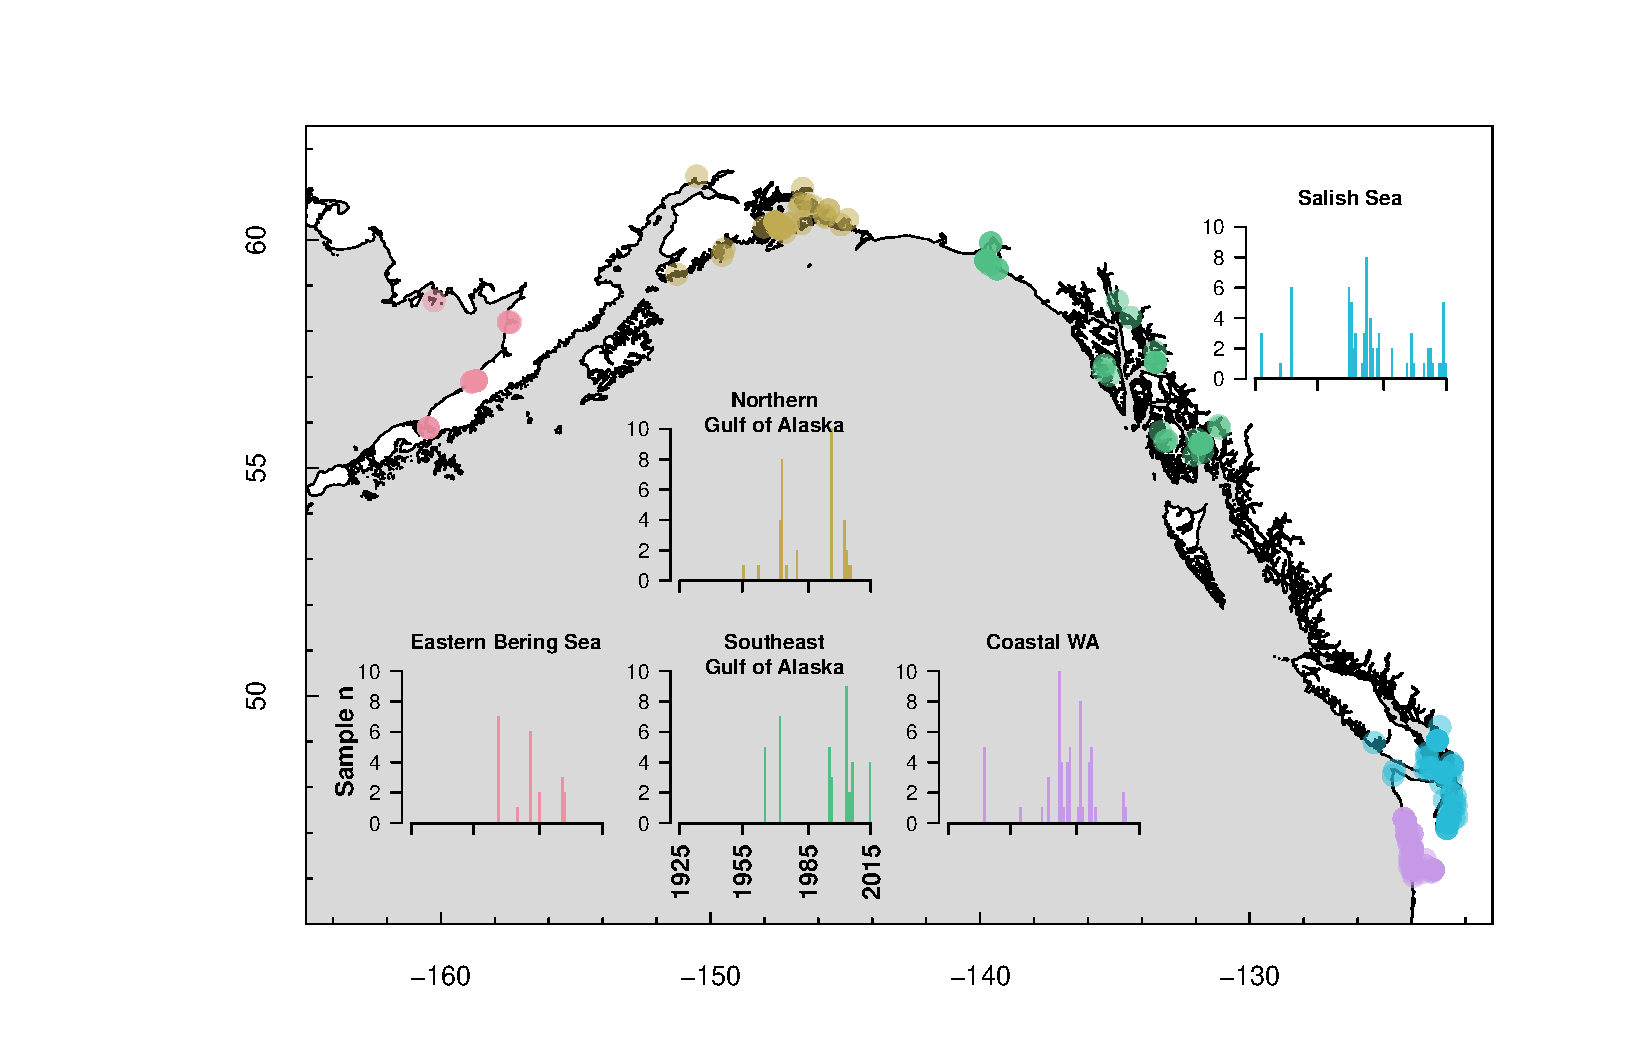
\includegraphics[width=0.95\textwidth]{figure/Ch2/Fig2_Map.pdf}
  \caption{Distribution of harbor seal specimens}
  \label{fig:map}
\end{figure}
\clearpage

\textbf{Figure} \ref{fig:dist}: Variability in \(\delta^{15}N_{Phe}\)
and \(\delta^{13}C\) values based on sub region and sex. * denotes a
significant difference in isotopic signature between males and females
for that region (colors correspond to \ref{fig:map}). \newline 
\begin{figure}[h]
\centering
  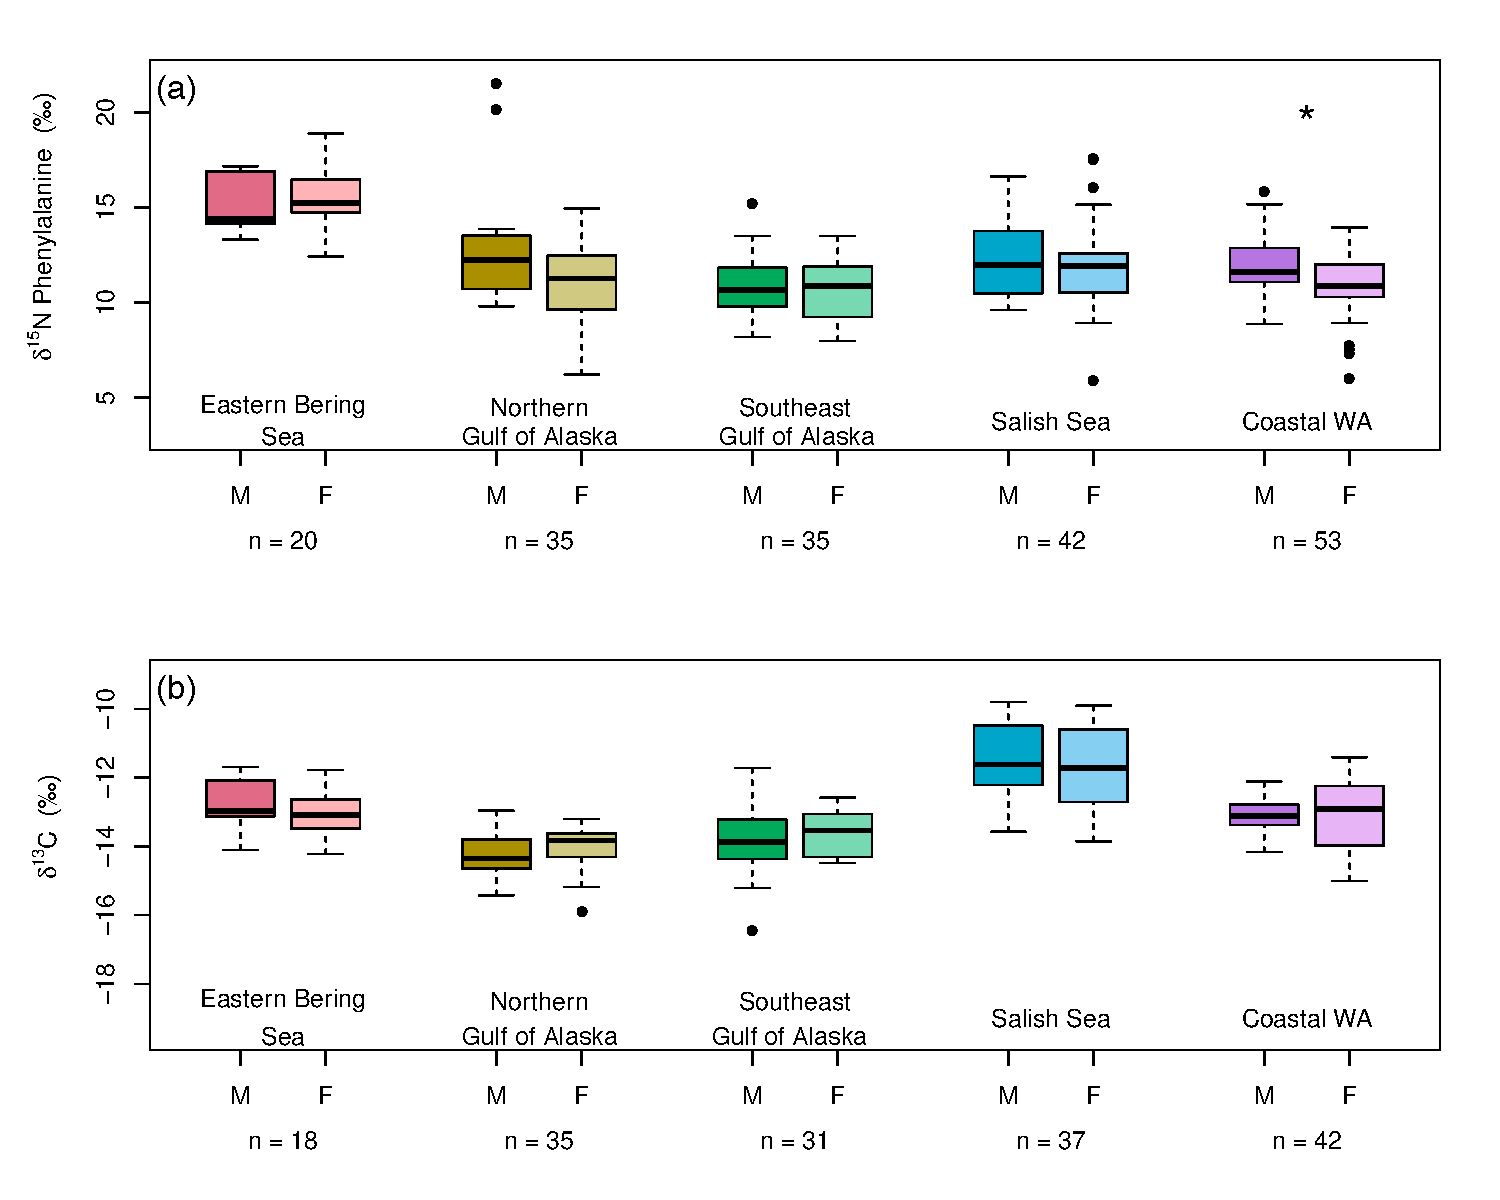
\includegraphics[width=1\textwidth]{figure/Ch2/Figure3_SexLocation.pdf}
  \caption{Sex and Region based differences}
  \label{fig:dist}
\end{figure}
\clearpage

\textbf{Figure} \ref{fig:hiermod}: Relationship between nitrogen sources
(\(\delta^{15}N_{Phe}\)) and primary production (\(\delta^{13}C\))
assimilated into the food web for A. a single linear model for the
combined data across the northeast Pacific and eastern Bering Sea and B.
a mixed effects model with random slope and intercept by sub region
(colors correspond to \ref{fig:map}). \newline 
\begin{figure}[h]
\centering
  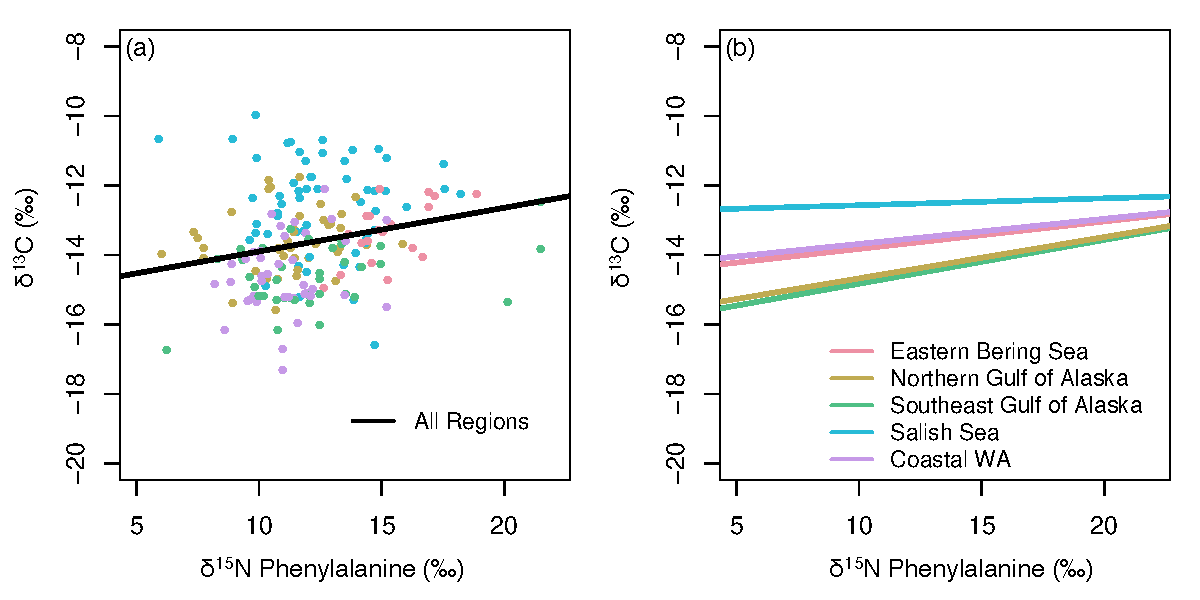
\includegraphics[width=1\textwidth]{figure/Ch2/hiermod.pdf}
  \caption{Hierarchical $\delta^{15}N_{Phe}$ and $\delta^{13}C$ Models}
  \label{fig:hiermod}
\end{figure}
\clearpage

\textbf{Figure} \ref{fig:coefres}: Coefficients of environmental
covariates for models with relative support (\(\Delta AIC_c\)
\textless{} 2) for harbor seal \(\delta^{15}N_{Phe}\) and
\(\delta^{13}C\) values in three regions of the northeast Pacific:
Washington, Gulf of Alaska, and the eastern Bering Sea. Color indicates
model support based on AIC\textsubscript{c} weight, points are the
coefficient estimates for each environmental covariate included in an
individual model, and bars show two standard deviations from the
coefficient estimate. \newline 
\begin{figure}[h]
\centering
  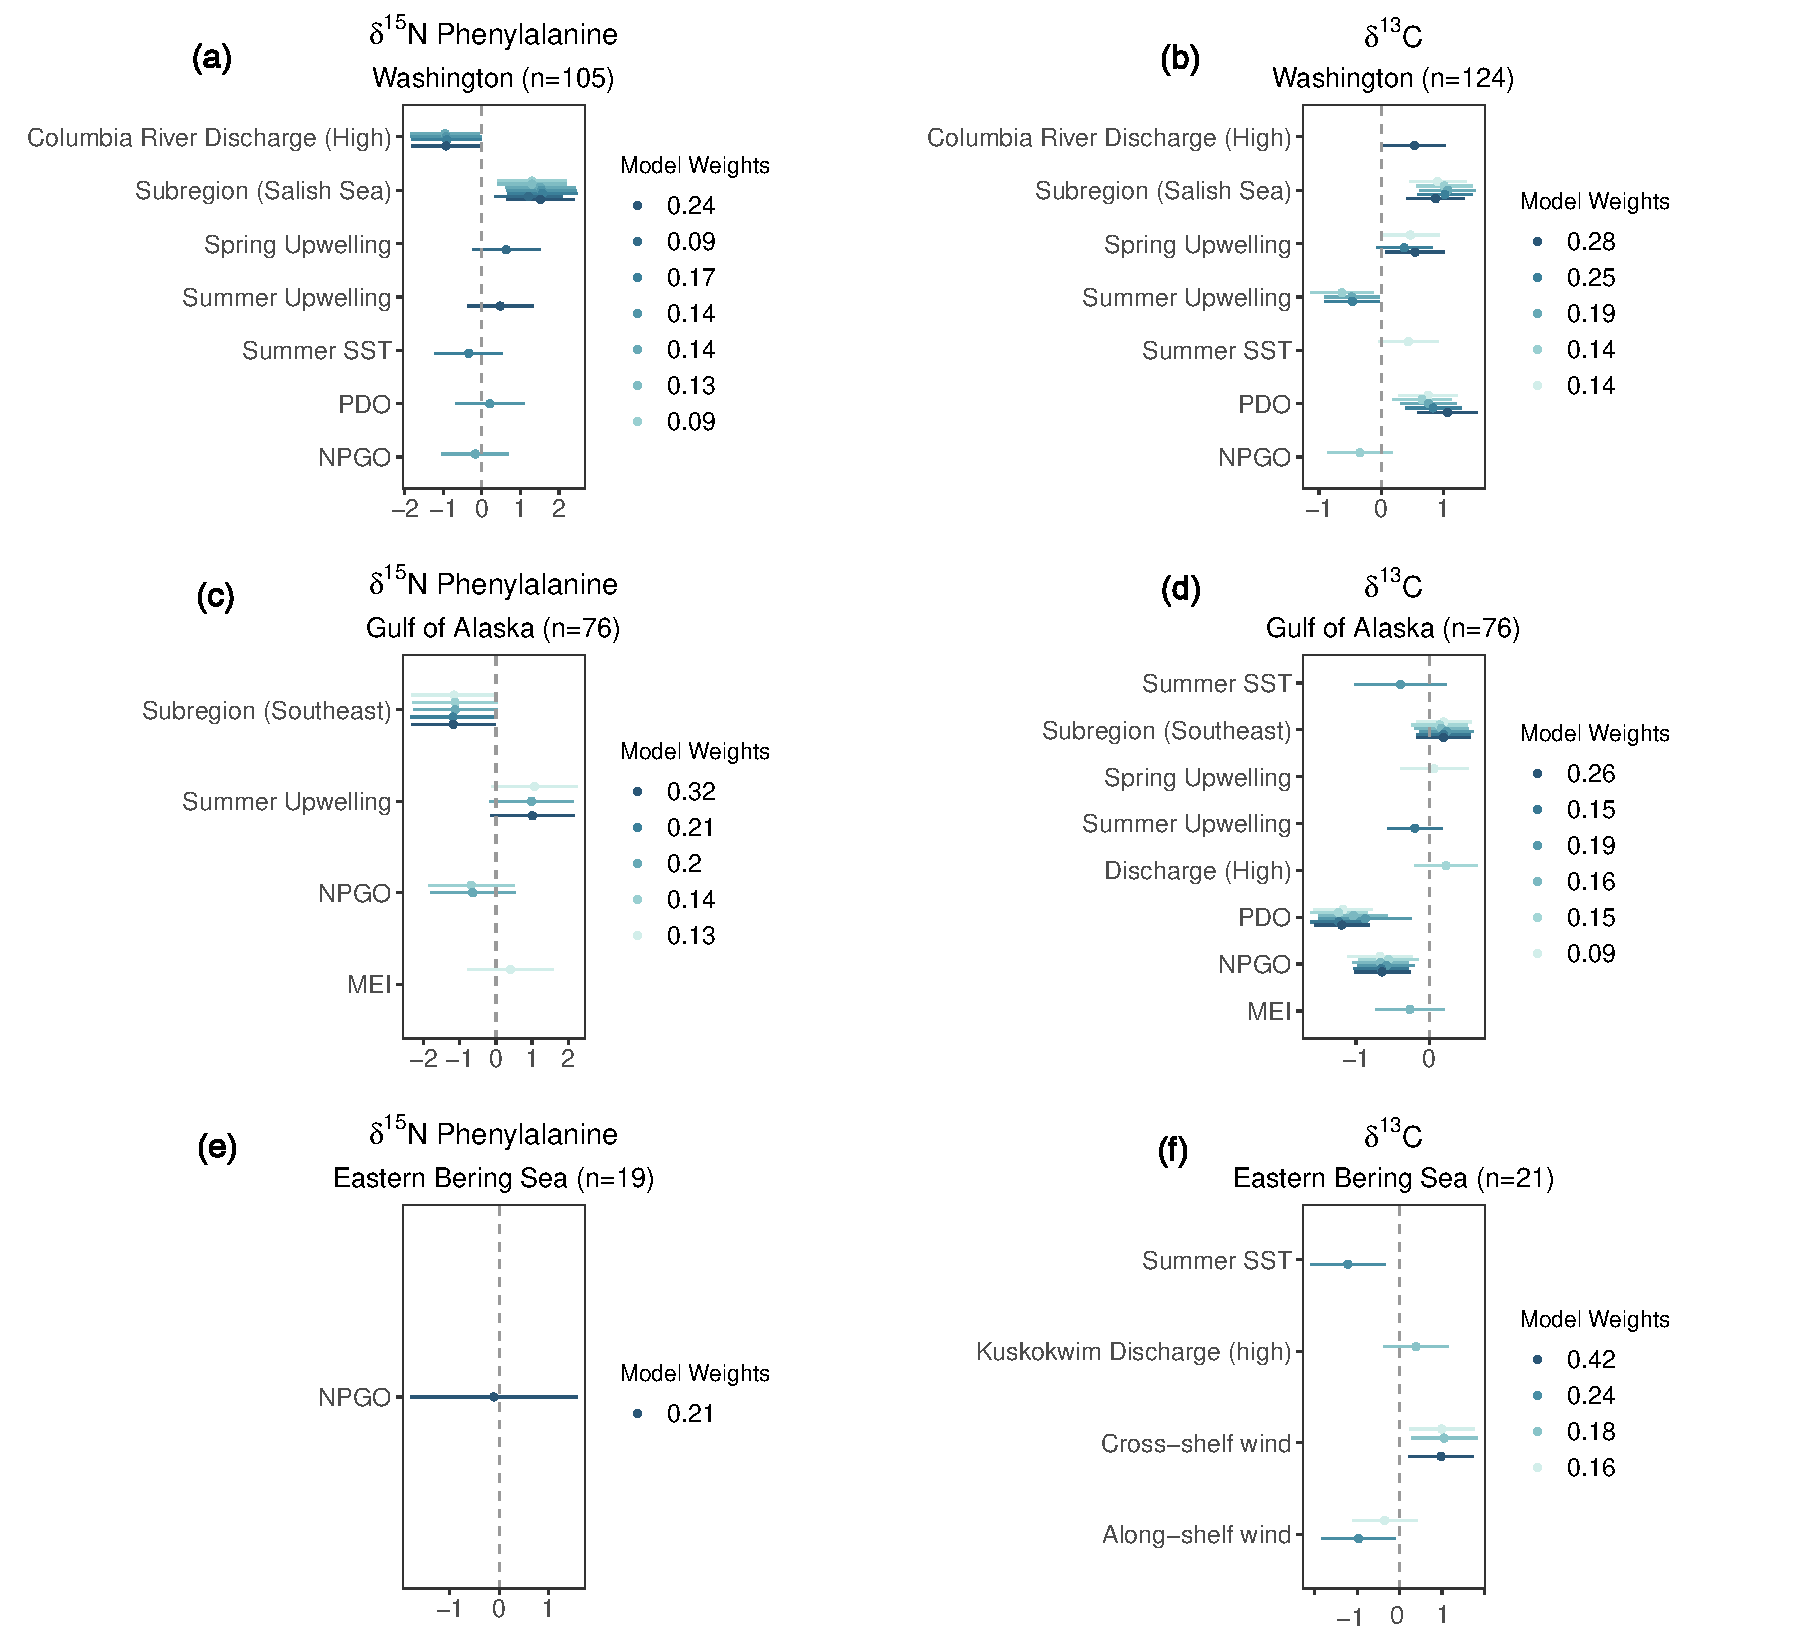
\includegraphics[width=0.9\textwidth]{figure/Ch2/Figure5_CoefPlot.pdf}
  \caption{Coefficients of Evironmental Covariates}
  \label{fig:coefres}
\end{figure}
\clearpage

\textbf{Figure} \ref{fig:GDFAAK}: Common trends in environmental
condition and food web assimilated stable isotope values for the
regional Gulf of Alaska gaussian-dynamic factor analysis model. The
solid lines represent the modelled trends, where 0 is the long-term
average and 1 and -1 represent the maximum and minimum possible values
respectively; the dash line is the 90\% credible interval. Factor
loadings can be interpreted as coefficients, representing the strength
of association between the modelled trend and each observed
environmental time series (colors represent a priori driver category).
Values close to 0 mean the observed time series did not correlate to the
corresponding trend, while values close to 1 show the observed time
series closely matched the modelled trend. Negative loadings indicate an
inverse relationship between the observed time series and modelled
trend. Stable isotope times series are modelled separately for the
northern (N. \(\delta^{15}N_{Phe}\); N. \(\delta^{13}C\)) and southeast
(S. \(\delta^{15}N_{Phe}\); S. \(\delta^{13}C\)) subregions.\\
\newline 
\begin{figure}[h]
\centering
  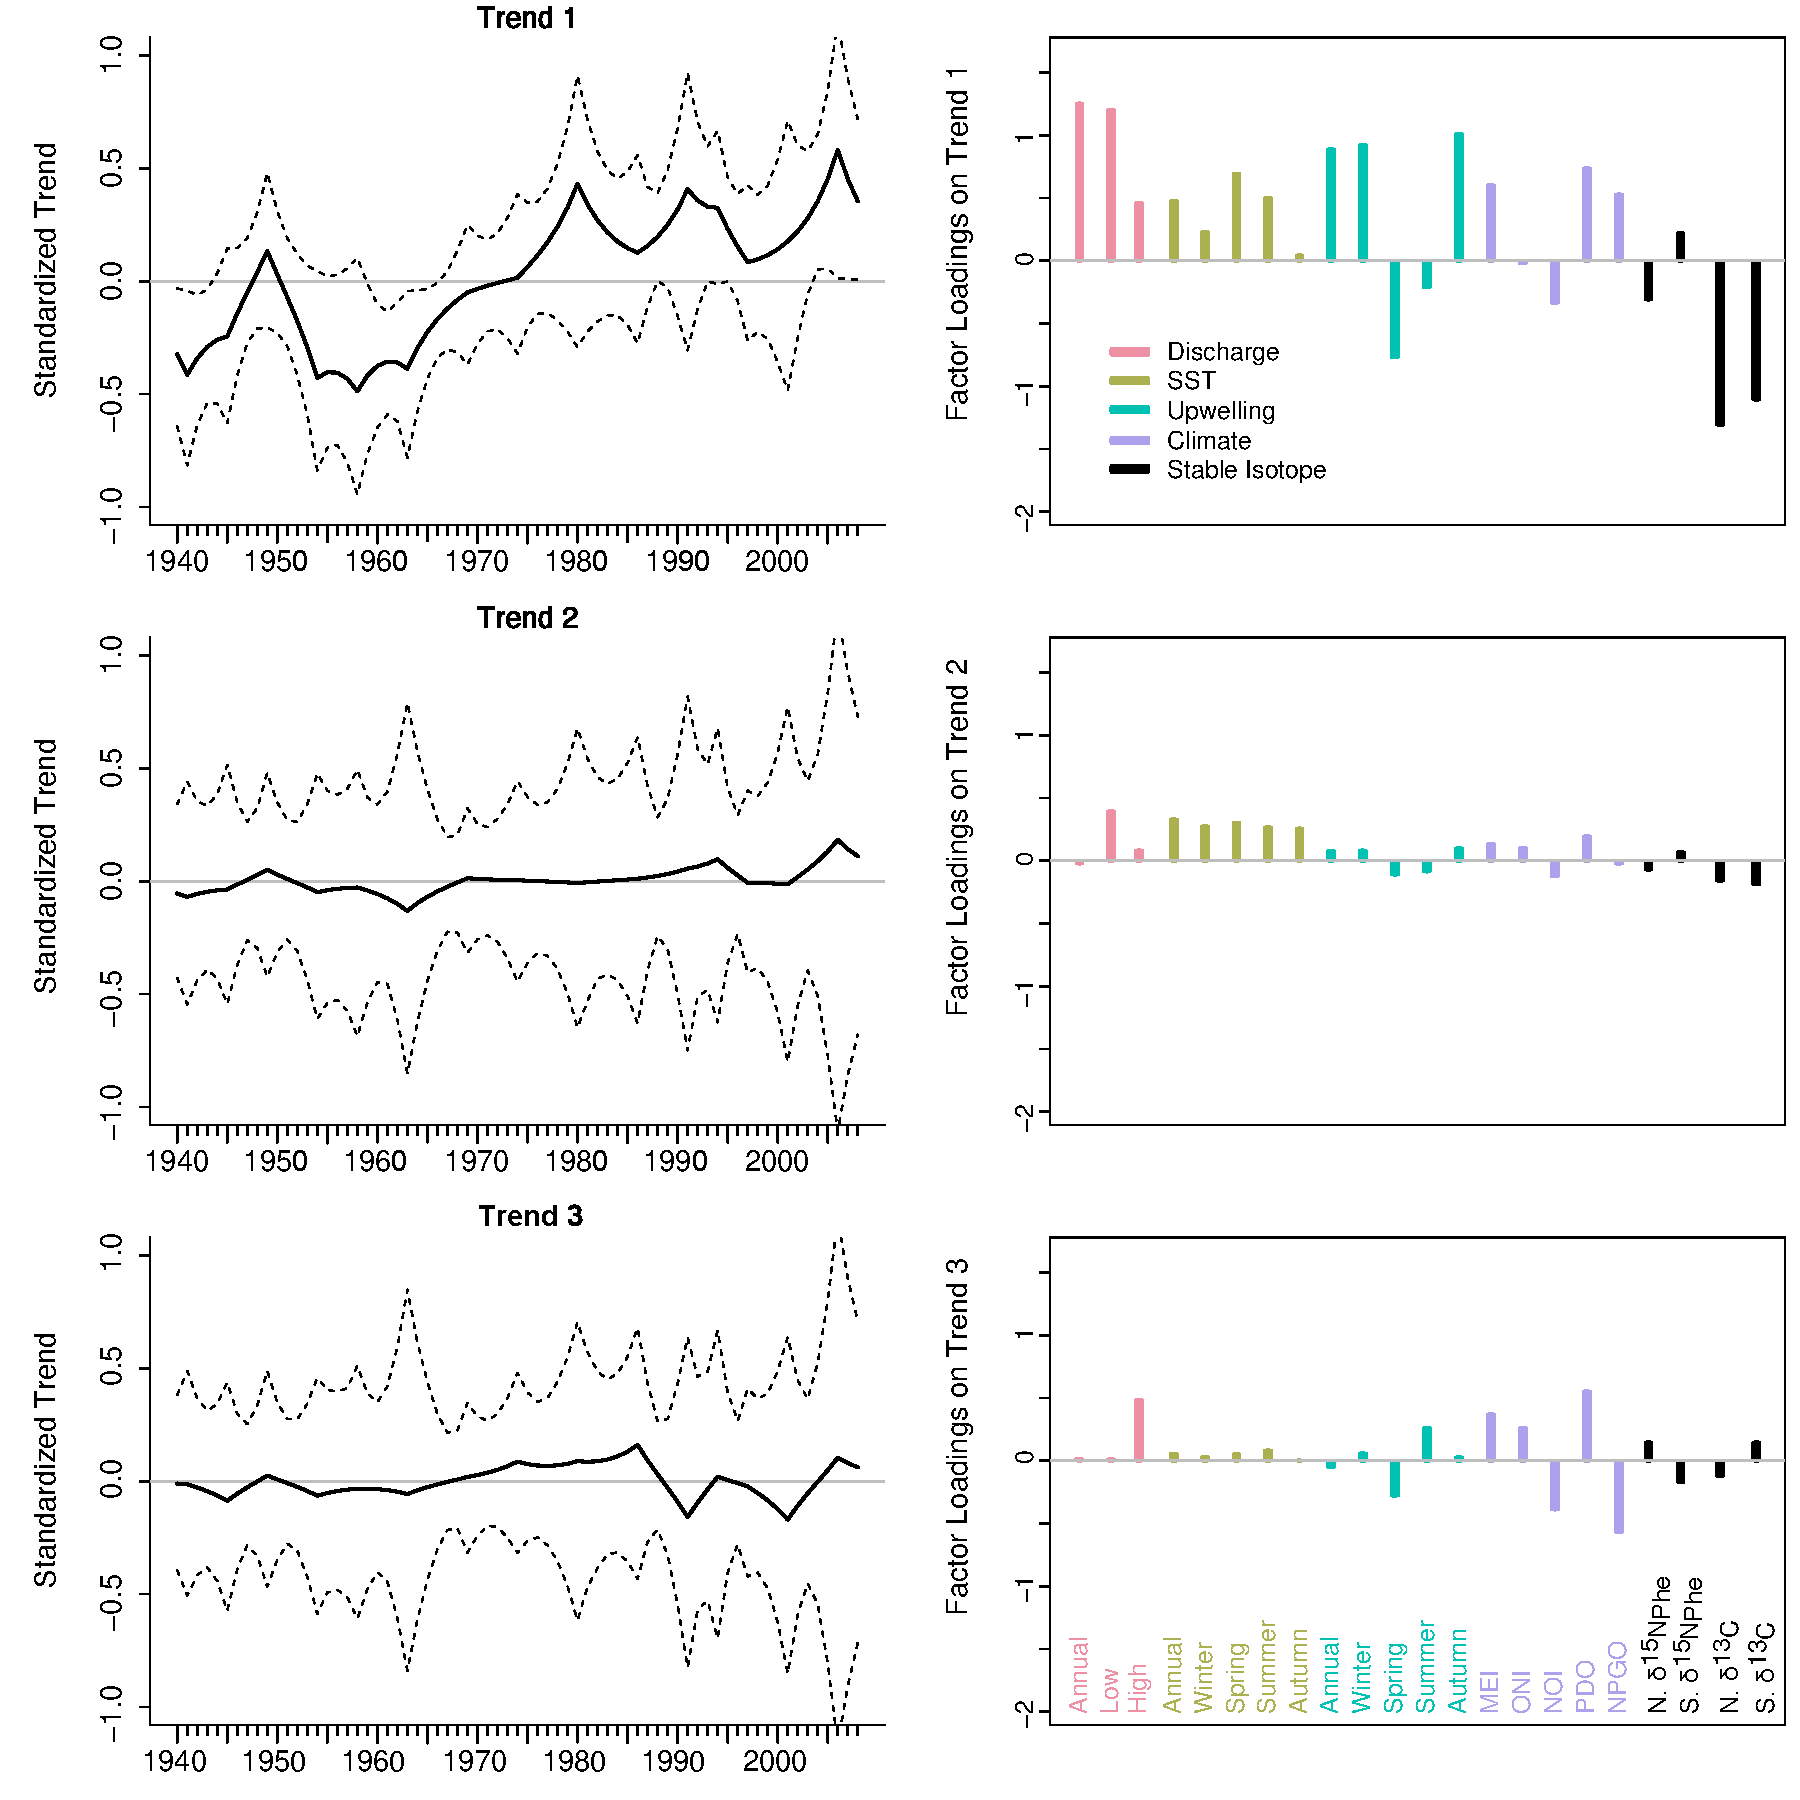
\includegraphics[width=0.9\textwidth]{figure/Ch2/Figure6_AK.GDFA.pdf}
  \caption{Alaska GDFA Results}
  \label{fig:GDFAAK}
\end{figure}
\clearpage

\textbf{Figure} \ref{fig:GDFAWA}: Common trends in environmental
condition and food web assimilated stable isotope values for the
regional Washington gaussian-dynamic factor analysis model. Stable
isotope times series are modelled separately for the coastal (C.
\(\delta^{15}N_{Phe}\); C. \(\delta^{13}C\)) and Salish Sea (S.S.
\(\delta^{15}N_{Phe}\); S.S. \(\delta^{13}C\)) subregions. See
\ref{fig:GDFAAK} caption for further interpretation.\\
\newline 
\begin{figure}[h]
\centering
  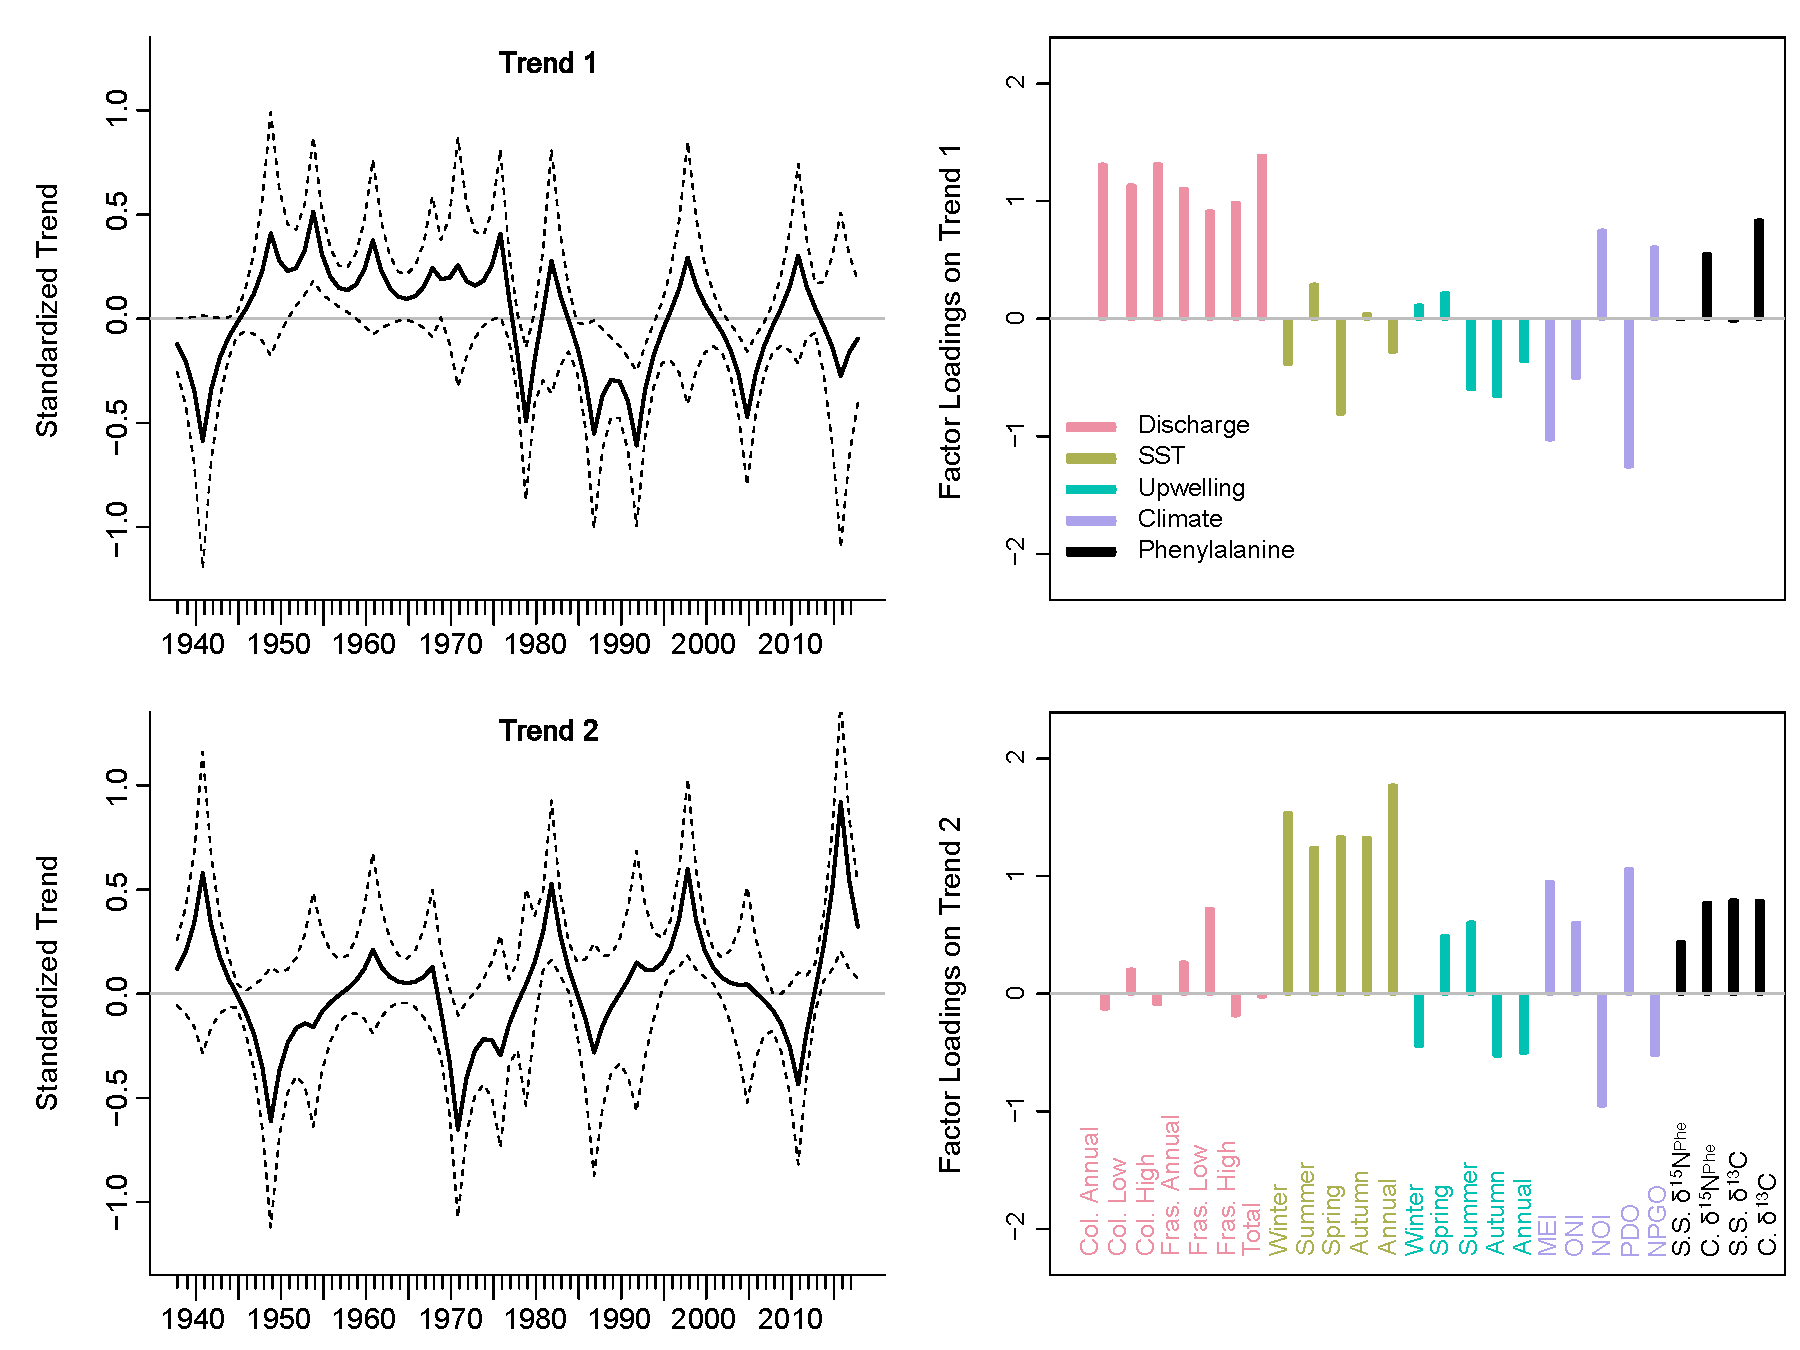
\includegraphics[width=0.9\textwidth]{figure/Ch2/Figure7_WA.GDFA.pdf}
  \caption{Washington GDFA Results}
  \label{fig:GDFAWA}
\end{figure}
\clearpage

\textbf{Figure} \ref{fig:Month}: Analysis of a) \(\delta^{15}N_{Phe}\)
and b) \(\delta^{13}C\) values by month. For both models, s(month) p
\textgreater{} 0.1 indicating no seasonality of harbor seal bone
collagen stable isotope signature.\\
\newline 
\begin{figure}[h]
  \centering
  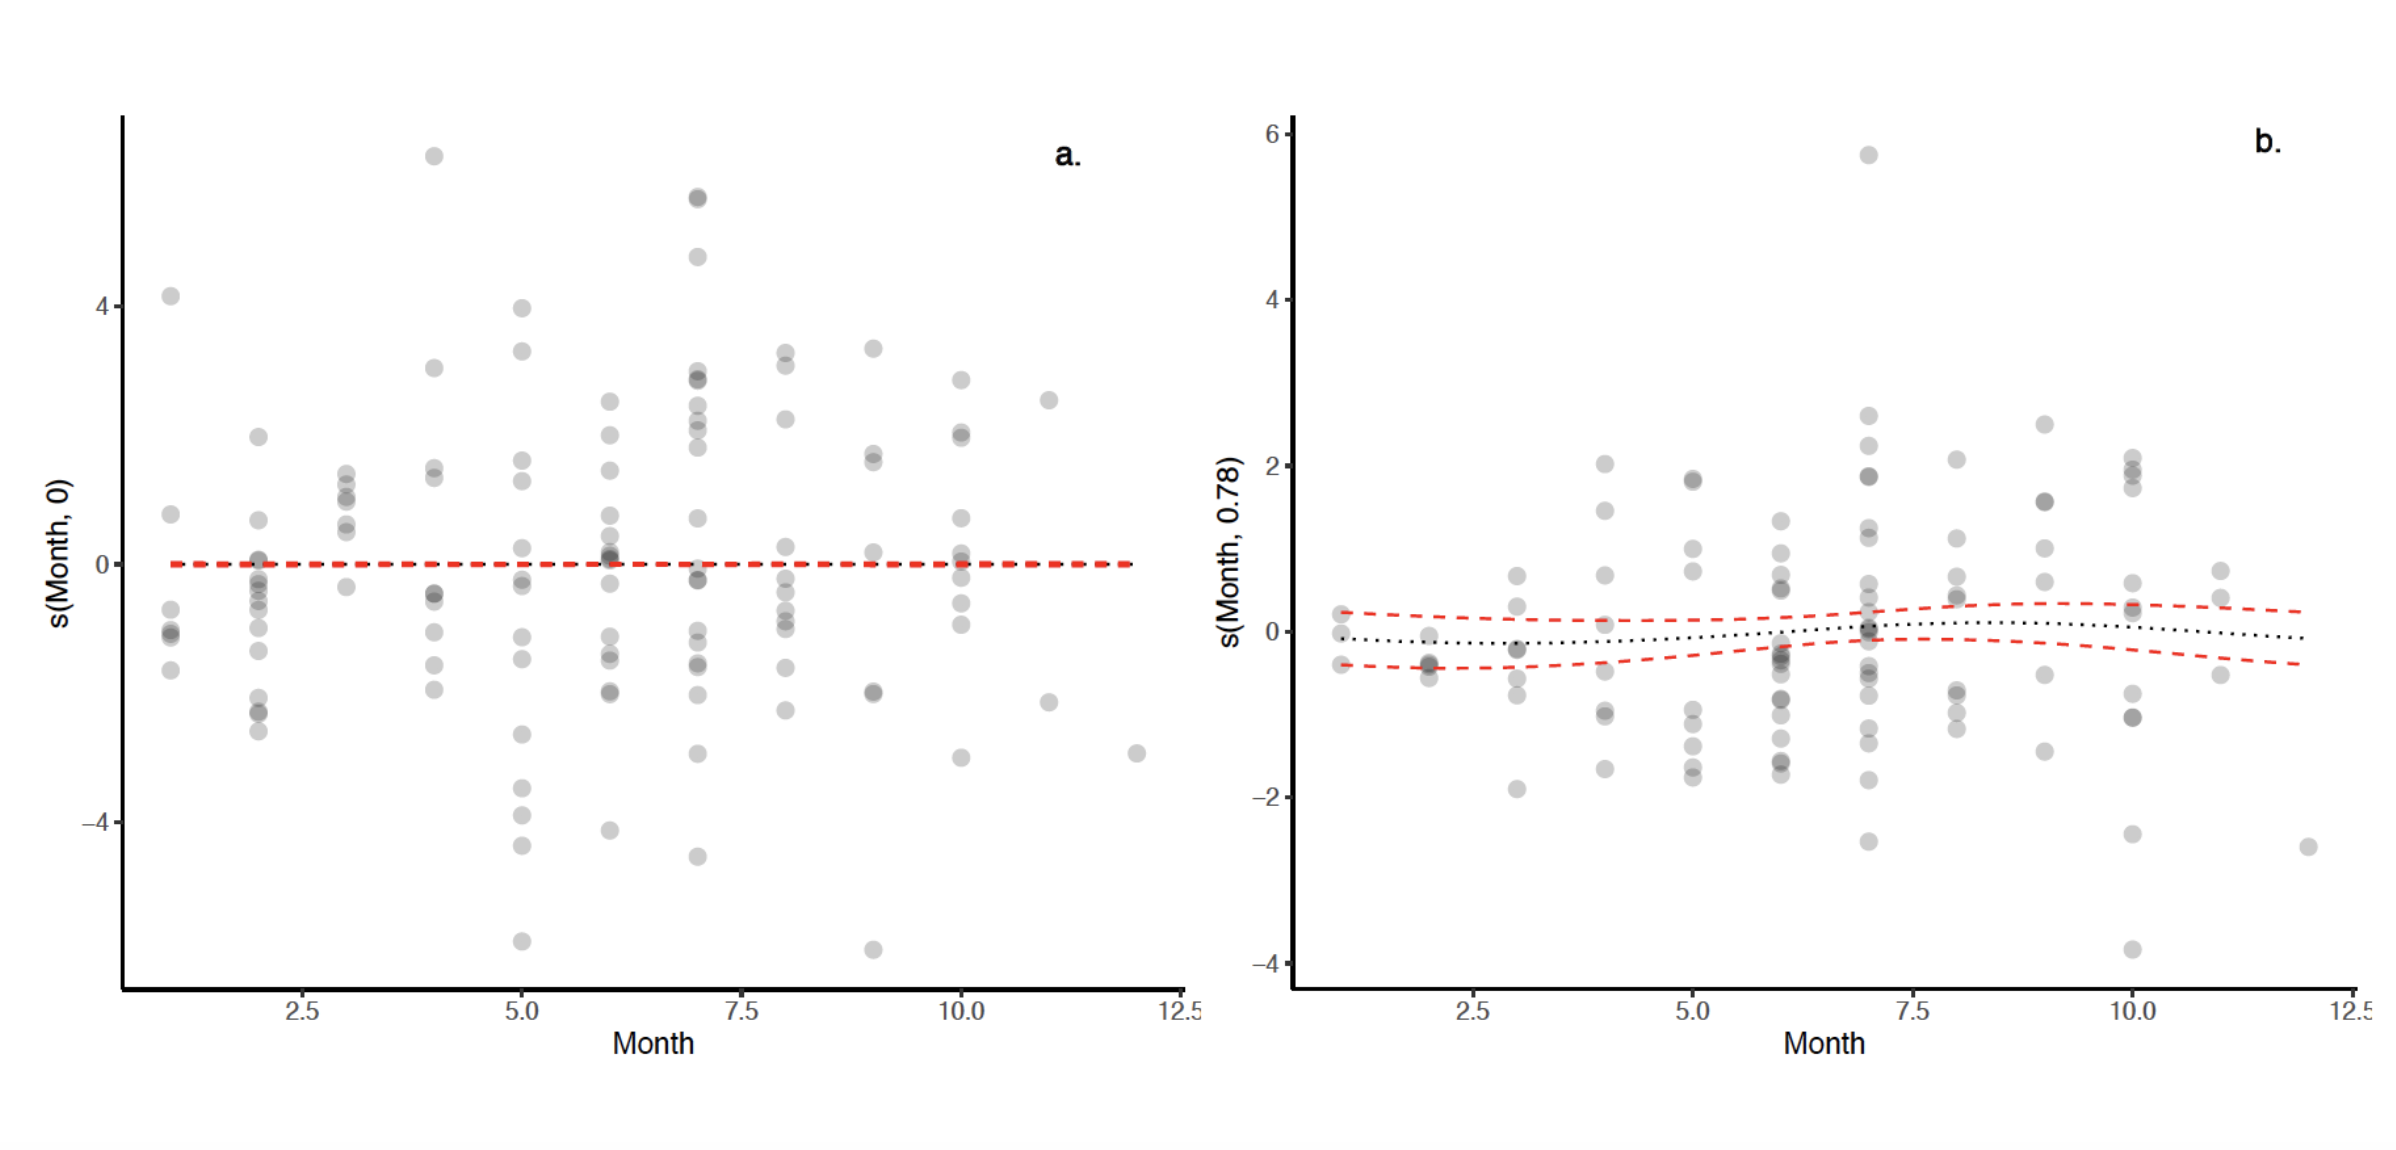
\includegraphics[width=0.8\textwidth]{figure/Ch2/figures2.png}
  \caption{Bone collagen stable isotope seasonality analysis}
  \label{fig:Month}
\end{figure}
\clearpage

\textbf{Figure} \ref{fig:Length}: Analysis of a) \(\delta^{15}N_{Phe}\)
and b) \(\delta^{13}C\) values by length. For both models, there was no
significant slope (p\textgreater{}0.1) \newline 
\begin{figure}[h]
\centering
  \includegraphics[width=0.8\textwidth]{figure/Ch2/FigureS2.pdf}
  \caption{Bone collagen stable isotope length analysis}
  \label{fig:Length}
\end{figure}
\clearpage

\textbf{Figure} \ref{fig:TSphe}: Bone collagen \(\delta^{15}N\) values
of phenylalanine from archival harbor seal specimens collected in the
northeastern Pacific in five subregions. \newline 
\begin{figure}[h]
\centering
  \includegraphics[height=0.8\textwidth]{figure/Ch2/FigureS3.pdf}
  \caption{Time series of $\delta^{15}N_{Phe}$ data}
  \label{fig:TSphe}
\end{figure}
\clearpage

\textbf{Figure} \ref{fig:nonSuess}: Bone collagen bulk \(\delta^{13}C\)
values of archival harbor seal specimens collected in the northeastern
Pacific in five subregions.These values are not corrected for the Suess
effect. \newline 
\begin{figure}[h]
\centering
  \includegraphics[height=0.8\textwidth]{figure/Ch2/FigureS4.pdf}
  \caption{Time series of $\delta^{13}C$ data}
  \label{fig:nonSuess}
\end{figure}
\clearpage

\textbf{Figure} \ref{fig:Suess}: Bone collagen bulk \(\delta^{13}C\)
values of archival harbor seal specimens collected in the northeastern
Pacific in five subregions.These values are corrected for the Seuss
effect. \newline 
\begin{figure}[h]
\centering
  \includegraphics[height=0.8\textwidth]{figure/Ch2/FigureS5.pdf}
  \caption{Time series of $\delta^{13}C$ data corrected for Suess effect}
  \label{fig:Suess}
\end{figure}
\clearpage

\textbf{Figure} \ref{fig:bulkN}: Bone collagen bulk \(\delta^{15}N\)
values of archival harbor seal specimens collected in the northeastern
Pacific in five subregions. \newline 
\begin{figure}[h]
\centering
  \includegraphics[height=0.8\textwidth]{figure/Ch2/FigureS6.pdf}
  \caption{Time series of bulk $\delta^{15}N$ data}
  \label{fig:bulkN}
\end{figure}
\clearpage

\textbf{Figure} \ref{fig:linresid}: Residuals for the model with the
most support (\ref{fig:coefres}) plotted by year. A trend in model
residuals would indicate environmental variables do not account for all
temporal variation in harbor seal \(\delta^{15}N_{Phe}\) and
\(\delta^{13}C\) values. \newline 
\begin{figure}[h]
\centering
  \includegraphics[height=0.85\textwidth]{figure/Ch2/FigureS7.pdf}
  \caption{Residuals trends for linear models with the most support}
  \label{fig:linresid}
\end{figure}
\clearpage

Figure 2.15: Model residual plots for the models with the most support
from the candidate model set. Note: EBS phenylalanine is an intercept
only model, GOA phenylalanine only contains a 2-factor location as a
covariate. \newline 
\begin{figure}[h]
\centering
  \includegraphics[height=0.8\textwidth]{figure/Ch2/FigureS8.pdf}
  \caption{Residuals for linear models with the most support}
  \label{fig:linresid2}
\end{figure}
\chapter{Delayed trophic response of a marine predator to ocean
condition and prey availability during the past
century}\label{delayed-trophic-response-of-a-marine-predator-to-ocean-condition-and-prey-availability-during-the-past-century}

\section{Abstract}\label{abstract-2}

Understanding the response of predators to ecological change at multiple
temporal scales can elucidate critical predator-prey dynamics that would
otherwise go unrecognized. We performed compound-specific nitrogen
stable isotope analysis (CSIA) of amino acids on 153 harbor seal museum
skull specimens to determine how this marine predator has responded to
ecosystem change over the past century. The relationships between harbor
seal trophic position, ocean condition, and prey abundance, were
analyzed using hierarchical modelling of a multi-amino acid framework
and applying 1-, 2-, and 3- year temporal lags. We identified delayed
responses of harbor seal trophic position to both physical ocean
conditions (upwelling, sea surface temperature, freshwater discharge)
and prey availability (Pacific hake, Pacific herring and Chinook
salmon). However, the magnitude and direction of the trophic response to
ecological changes depended on the temporal delay. For example, harbor
seal trophic position was negatively associated with summer upwelling,
but had a 1- year delayed response to summer sea surface temperature,
indicating some predator responses to climate extremes are not
immediately observable. These results highlight the importance of
considering dynamic responses of predators to their environment as
multiple ecological factors are often changing simultaneously and
predator response occurs at multiple temporal scales.

\section{Introduction}\label{introduction-3}

The regulation of food web structure by resources (bottom-up control)
and the presence of top predators (top-down control) is fundamental for
understanding food web responses to environmental, ecological, and
anthropogenic change (S. R. Carpenter, Kitchell, \& Hodgson,
\protect\hyperlink{ref-Carpenter1985}{1985}; Estes, Tinker, Williams, \&
Doak, \protect\hyperlink{ref-Estes1998}{1998}; Hunter \& Price,
\protect\hyperlink{ref-Hunter1992}{1992}). Ecological communities are
continuously experiencing both biotic and abiotic disturbances (Paine,
Tegner, \& Johnson, \protect\hyperlink{ref-Paine1998}{1998}) and the
ability of food webs to dynamically respond to these changes is crucial
for ecosystem stability (Ghedini, Russell, \& Connell,
\protect\hyperlink{ref-Ghedini2015}{2015}). In marine food webs,
physical ocean conditions can impact primary production and ultimately
constrain energy availability and thus biomass at higher trophic levels
(Emmanuel Chassot et al., \protect\hyperlink{ref-Chassot2010}{2010}; J.
K. Moore et al., \protect\hyperlink{ref-Moore2018}{2018}; Ware \&
Thomson, \protect\hyperlink{ref-Ware2005}{2005}). Similarly, the removal
of top predators from an ecosystem as a result of human activities such
as fishing can decrease predation pressure and alter abundance in both
adjacent and non-adjacent trophic levels (Heithaus, Frid, Wirsing, \&
Worm, \protect\hyperlink{ref-Heithaus2008}{2008}; Steneck,
\protect\hyperlink{ref-Steneck2012}{2012}). However, large-scale changes
in nutrient availability (Rykaczewski \& Dunne,
\protect\hyperlink{ref-Rykaczewski2010}{2010}), primary productivity
(Emmanuel Chassot et al., \protect\hyperlink{ref-Chassot2010}{2010}),
and top predator abundance over the past century (Magera, Flemming,
Kaschner, Christensen, \& Lotze,
\protect\hyperlink{ref-Magera2013}{2013}) means many food webs are
experiencing shifts in multiple mechanisms of regulation in tandem,
making it challenging to identify dominant drivers structuring
ecosystems over the long term.

Marine predators respond to multiple types of bottom-up drivers (i.e.,
ocean condition, prey availability) and the different temporal scales
over which they respond is crucial for understanding community
stability. However, delayed predator responses to environmental
perturbations are prevalent in marine system, as impacts do not
immediately propagate through the complete food web (Duguid et al.,
\protect\hyperlink{ref-Duguid2019}{2019}; R. S. Smith, Weldon, Hayward,
\& Henson, \protect\hyperlink{ref-Smith2017}{2017}). Given communities
can shift from bottom-up to top-down control, particularly in response
to changing climate conditions (Kratina, Greig, Thompson,
Carvalho-Pereira, \& Shurin, \protect\hyperlink{ref-Kratina2012}{2012}),
delayed predator responses to climate conditions has implications for
abundance and mortality rates of prey.

Historical marine predator data that span multiple environmental,
ecological, and anthropogenic contexts are useful for identifying time
scales over which predators respond to ecosystem drivers.
Compound-specific stable isotope analysis (CSIA) of amino acid nitrogen
can serve as a tracer of historical predator response to ecological and
environmental change by deriving retrospective trophic position
estimates from museum specimens (Feddern, Holtgrieve, \& Ward,
\protect\hyperlink{ref-Feddern2021}{2021}; McMahon et al.,
\protect\hyperlink{ref-McMahon2019}{2019}). Source amino acids (i.e.,
phenylalanine, lysine, methionine) exhibit minimal trophic
discrimination (the difference in
\textsuperscript{15}N/\textsuperscript{14}N between trophic and source
amino acids in consumers from a trophic transfer) and thus are a proxy
for the isotopic signature of primary producers at the base of the food
web. In contrast, trophic amino acids (i.e., alanine, glutamic acid,
valine, proline) demonstrate trophic enrichment (Kelton \& Matthew,
\protect\hyperlink{ref-McMahon2016}{2016}) that varies for individual
amino acids. Combined, this approach allows for reconstruction of
historic trophic position estimates under changing environmental
conditions when characterizing the isotopic baseline of past ecosystems
may not be possible (McMahon et al.,
\protect\hyperlink{ref-McMahon2019}{2019}). Thus, CSIA is well suited to
identify long-term drivers of food web dynamics when analyzed with
historic indices of ocean condition and prey availability.

Reconstructing time series of predator trophic position requires careful
consideration of physiological and ecological parameters that contribute
to stable isotope signatures. First, taxa exhibit different trophic
enrichment factors based on excretion pathways, diet type (omnivory,
herbivory, carnivory), and growth (J. M. Nielsen, Popp, \& Winder,
\protect\hyperlink{ref-Nielsen2015}{2015}). Second, the nitrogen
production pathway of vascular (i.e., seagrasses) versus nonvascular
(i.e., marine diatoms) primary producers impart distinct stable isotope
fractionation factors (\(\beta\)) as inorganic sources of nitrogen are
converted to tissues (H. B. Vander Zanden et al.,
\protect\hyperlink{ref-VanderZanden2013}{2013}). Assumptions about the
relative contributions of vascular versus nonvascular plants can
therefore impact trophic position estimates (Choi et al. 2017). Finally,
there is a delay between the time a prey source is consumed and when
that prey source has been fully assimilated into the consumer, referred
to as the `turnover time'. Turnover times must be considered when
comparing trophic position data to ocean condition and prey availability
covariates, as the consumer response to an ecological change will not be
immediately observable in consumer tissues.

Nearshore coastal ecosystems provide a model system to assess long-term
changes of food web drivers using archival museum specimens of a marine
predator by applying CSIA. Food webs of coastal Washington and the
Salish Sea have experienced dramatic restructuring over the past century
due to declines and subsequent recoveries of marine predators (S.
Jeffries, Huber, Calambokidis, \& Laake,
\protect\hyperlink{ref-Jeffries2003}{2003}; Ohlberger, Schindler, Ward,
Walsworth, \& Essington, \protect\hyperlink{ref-Ohlberger2019}{2019}).
Decades of state-financed population control programs resulted in harbor
seals (\emph{Phoca vitulina}) reaching a historic low in the 1970's,
with an estimated abundance of approximately 1,000 individuals (S.
Jeffries et al., \protect\hyperlink{ref-Jeffries2003}{2003}). Following
the cessation of bounties in 1960 and the passage of the Marine Mammal
Protection Act in 1972, top-predator abundance increased dramatically.
Benefitting from a relatively short life history, generalist diet, and
legislation restricting mortality, harbor seal populations increased
10-fold between 1970 and 2003 (S. Jeffries et al.,
\protect\hyperlink{ref-Jeffries2003}{2003}). The dramatic increase in
abundance of this top predator has been implicated in the declines in
economically and ecologically important prey species in the region
(Chasco et al., \protect\hyperlink{ref-Chasco2017}{2017}; Nelson,
Walters, Trites, \& McAllister,
\protect\hyperlink{ref-Nelson2019}{2019}), specifically, Chinook salmon
(\emph{Oncorhynchus tshawytscha}). Chinook salmon are listed as
endangered in the region (WDFW 2017) and are an important prey species
for the endangered southern resident orca (Marshall, Stier, Samhouri,
Kelly, \& Ward, \protect\hyperlink{ref-Marshall2016}{2016}).
Simultaneously, the region has also experienced changes in nutrients
(Mohamedali et al. 2011), climate regimes (Corwith \& Wheeler,
\protect\hyperlink{ref-Corwith2002}{2002}; Mantua \& Hare,
\protect\hyperlink{ref-Mantua2002}{2002}) and abundances of other
important prey species such as Pacific herring (\emph{Clupea pallasii},
Siple \& Francis (\protect\hyperlink{ref-Siple2015}{2015})).

Here we examined a century of harbor seal trophic position data in
coastal Washington and the Salish Sea. The objective of this work is to
identify the time scales at which physical ocean conditions and prey
availability exert bottom-up control on marine predator trophic ecology.
We assumed a correlation between trophic position and prey species
abundance is the result of increased or decreased consumption of that
species. Additionally, we established a multi-amino acid framework for
measuring trophic position that improves precision and ecological
accuracy by applying a species-specific trophic discrimination factor
(McMahon et al., \protect\hyperlink{ref-McMahon2019}{2019}; J. M.
Nielsen et al., \protect\hyperlink{ref-Nielsen2015}{2015}). We also
included a system specific \(\beta\) value rather than a universal
value, and applied temporal lags to account for both physiological and
ecological delays in consumer response.

\section{Methods}\label{methods-2}

\subsection{Sample collection and
analysis}\label{sample-collection-and-analysis-1}

Samples were obtained using methods described in Feddern et al.
(\protect\hyperlink{ref-Feddern2021}{2021}). Briefly, harbor seal bone
was obtained from four museum institutions (the Burke Museum, the Slater
Museum, the Royal British Columbia Museum, and the Smithsonian
Institute) and the National Marine Mammal Laboratory (NOAA). Specimens
were treated by maceration in warm water and stored in acid free boxes.
Sampling targeted adult specimens and prioritized long-term temporal
coverage in two main regions: coastal Washington and the Salish Sea
(which included 18 specimens from British Columbia). Specimens with sex,
length, and age data were also prioritized but this information was not
available for all sampled specimens. A total of 153 specimens were
sampled with field collection dates ranging 1928-2014 (Figure
\ref{fig:map3}).

\subsection{Trophic position
determination}\label{trophic-position-determination}

Bone collagen was decalcified, acid hydrolyzed, derivatized, and
analyzed for nitrogen CSIA (\(\delta^{15}N\)) of 12 individual amino
acids. Collagen samples were measured in triplicate with a laboratory
standard containing a 12 amino acid mixture of known isotopic
composition and a linear drift correction was applied. Full analytical
details are described in Appendix 1: Text 1. Previous controlled feeding
studies have determined the trophic enrichment factor (TEF) for harbor
seals is substantially lower than the conventional literature value of
7.6‰ (Germain et al., \protect\hyperlink{ref-Germain2013}{2013}) and
thus applying a harbor seal-specific TEF is more accurate (McMahon,
Polito, Abel, McCarthy, \& Thorrold,
\protect\hyperlink{ref-McMahon2015}{2015}). Therefore, trophic position
was calculated using a harbor seal-specific TEF, described by McMahon et
al. (\protect\hyperlink{ref-McMahon2015}{2015}) as a ``multi-TEF''
approach, using the following equation:
\begin{equation} 
Trophic Position =   
  \frac{\delta^{15}N_{(i-o)} - TEF_{(i-o),j} - \beta_{(i-o),N}}{\overline{TEF}_{(i-o)}}+2
  \label{eq:TP3}
\end{equation}
where \(\delta^{15}N_i\) is the measured stable isotope composition of a
trophic amino acid i in a sample and \(\delta^{15}N_o\) is the stable
isotope composition of a source amino acid o in a
sample.\(\delta^{15}N_{(i-o)}\) represents the total trophic enrichment
that has occurred throughout the food web measurable from predator
tissues. \(TEF_{(i-o),j}\) is the trophic enrichment factor between
trophic amino acid \emph{i} and source amino acid \emph{o} of a specific
consumer \emph{j} (in this study, harbor seals) which occurs when
consumer \emph{j} assimilates prey. \(\beta_{(i-o),N}\) is the
difference in enrichment between a specific trophic amino acid \emph{i}
and source amino acid o for non-vascular primary producers \emph{N} that
occurs when primary producers assimilate inorganic nitrogen (J. M.
Nielsen et al. (\protect\hyperlink{ref-Nielsen2015}{2015}); Table
\ref{tab:tpparam}). \(\overline{TEF}_{(i-o)}\) represents the mean
trophic enrichment that occurs at other trophic levels in the food web,
and is calculated from the mean difference between trophic amino acid i
and source amino acid o across all consumers described in J. M. Nielsen
et al. (\protect\hyperlink{ref-Nielsen2015}{2015}).

The \(\beta\) parameter differs substantially between vascular and
nonvascular primary producers (Ramirez, Besser, Newsome, \& McMahon
(\protect\hyperlink{ref-Ramirez2021}{2021}); Table \ref{tab:tpparam}).
In food webs that assimilate organic matter from both vascular and
nonvascular plants, including many nearshore food webs, \(\beta\) will
be intermediate. In addition to testing a value that represents
nonvascular primary producers exclusively \(\beta_{(i-o),N}\), we also
applied a two-source mixing model using carbon stable isotope data
similar to B. Choi et al. (\protect\hyperlink{ref-Choi2017}{2017}). This
generates a \(\beta\) that is weighted \(\beta_{(i-o),NV}\) based on the
contributions of both vascular and nonvascular plants specific to the
Washington nearshore ecosystem by first calculating the percent
contribution of vascular plants to the food web:
\begin{equation} 
  \% V =
    \frac{\delta^{13}C_{H} - \delta^{13}C_{N}}
    {\delta^{13}C_{V} - \delta^{13}C_{N}}/100
    \label{eq:perV}
\end{equation}
where \(\delta^{13}C_{H}\) is the mean observed \(\delta^{13}C\) value
for Washington harbor seals. \(\delta^{13}C_{V}\) is the carbon stable
isotope end member for vascular plants, v (-9.5 ‰, derived from
seagrasses \emph{Zostera spp.}); and \(\delta^{13}C_{N}\) is the carbon
stable isotope end member for nonvascular plants, n (-19.5‰, derived
from phytoplankton). Carbon end members were specific to the Washington
nearshore ecosystems (Howe \& Simenstad,
\protect\hyperlink{ref-Howe2015}{2015}). Percent V is the percent
contribution of vascular plants to the food web in which harbor seals
forage. This assumes the trophic enrichment of \(^{13}C\) is generally
negligible (0--1‰, Deniro \& Epstein 1978). \(\beta_{(i-o),NV}\) was
then derived by:
\begin{equation} 
\beta_{(i-o),NV} = (\beta_{(i-o),V}*\%V) +
(\beta_{(i-o),N}*(1-\%V))
  \label{eq:betanv}
\end{equation}
where \(\beta_{(i-o),N}\) is the enrichment between an individual
trophic amino acid \emph{i} and source amino acid \emph{o} for aquatic
phytoplankton and \(\beta_{(i-o),V}\) represents the trophic enrichment
of seagrass which are vascular plants (Table \ref{tab:tpparam}).

\subsection{Quantifying bottom-up drivers of
foraging}\label{quantifying-bottom-up-drivers-of-foraging}

To identify the most important explanatory variables of ocean condition
and prey availability on predator trophic position, we fit two sets of
candidate models using a multi-amino acid (glutamic acid, aspartic acid,
alanine, proline, valine) hierarchical model. We selected 12 putative
explanatory variables based on the length of the time series and divided
them \emph{a priori} into our two categories of interest, ocean
condition and prey availability, representing our expected primary
forcing mechanisms (Tables 3.2 \& 3.4). We fit candidate models to the
trophic position and covariate data, and the candidate model set
included a null and location-only model (Tables \ref{tab:ocmod} \&
\ref{tab:prmod}). Location (Salish Sea or coastal Washington) was
included as a factor in all candidate models except the null model. Due
to the correlation between the multivariate El Niño Southern Oscillation
index and the Pacific Decadal Oscillation only one of these covariates
were included in a single model. All timeseries were standardized around
a mean of 0 and standard deviation of 1. To avoid collinearity, no more
than four covariates (including location) were included in an individual
model.

J. M. Nielsen et al. (\protect\hyperlink{ref-Nielsen2015}{2015})
determined that the use of multiple amino acids improves estimates of
trophic position. Therefore, we used multiple trophic amino acids
\emph{i} (alanine, glutamic acid, valine and proline) and one source
amino acid \emph{o} (phenylalanine) to calculate trophic position. We
selected amino acids based on: their prevalence in previous studies to
derive parameters for equation 1; tissue turnover time relative to the
source amino acid, phenylalanine; and their concentrations in bone
collagen. The hierarchical linear model took the following structure:
\begin{equation} 
\boldsymbol{y}_t = \alpha_k + \boldsymbol{\beta} \boldsymbol{X}_{t-d} +\epsilon, 
  \label{eq:hier3}
\end{equation}
where \emph{y} represents harbor seal trophic position from year
\emph{t} and \emph{k} represents four different trophic amino acids
(factors) used to calculate trophic position included as a random
effects. \(\boldsymbol{X}\) is a matrix of continuous bottom-up drivers
in year \emph{t}. \(\boldsymbol{\beta}\) is a vector of predicted
effects (coefficients) of bottom-up drivers included in the model
(Tables \ref{tab:ocmod} \& \ref{tab:prmod}) on harbor seal trophic
position, and \emph{a} is the predicted trophic position when all
included bottom-up drivers are at an average value (represented by 0) in
the coastal region of Washington. The variable \emph{d} is the temporal
lag between a change in bottom-up drivers and when that change is
reflected in harbor seal bone collagen. This lag can be due to both
physiological (tissue turnover) or ecological effects (rate of
propagation through the food web). Time (year, Figure \ref{fig:year}),
sex, size (Figures \ref{fig:sexWA} \& \ref{fig:lengthWA}), and
seasonality (month, Figure \ref{fig:season}), were also considered as
predictors of trophic position but no significant associations were
identified and thus these parameters were not included in the
hierarchical modeling (Appendix Text 2). The best performing models for
both of these approaches were selected using Akaike's Information
Criterion (Akaike 1973) with a correction for small sample size
(\(AIC_{c}\)). Inclusion of predictors in the model with the most
support is indicative of ecological parameters that alter harbor seal
foraging ecology or food web dynamics. Additionally, magnitude and sign
of the coefficients for included predictors can be interpreted as the
degree of trophic change induced by consuming different species, life
stages of species, or groups of species, caused by a given predictor.

Stable isotope composition of bone collagen is assumed to reflect diet
over the past 1-2 years of the individual's life (K. A. Hobson \& Clark,
\protect\hyperlink{ref-Hobson1992}{1992}; Newsome, Koch, Etnier, \&
Aurioles-Gamboa, \protect\hyperlink{ref-Newsome2006}{2006}; Riofrío-Lazo
\& Aurioles-Gamboa, \protect\hyperlink{ref-Riofrio2013}{2013}). A 1-year
lag (\emph{d}) was applied to all harbor seal trophic position estimates
to account for the physiological delay from tissue turnover time of bone
collagen, where the collagen in a harbor seal collected in year \emph{t}
reflects what the individual ate in the previous year, \emph{t}-1.
Delayed harbor seal foraging response to ecosystem dynamics was also
tested by applying additional 2-year and 3-year lags to trophic position
data; these models represent a 1-year and 2-year ecological delay in
addition to the 1-year physiological delay for tissue turnover time. For
example, the association between harbor seal trophic position and
environmental conditions 2 years before the collection year would
indicate that there was a 1-year delay between when the environmental
change happened and when the resultant changes propagated through the
food web, after accounting for the 1-year tissue turnover time. To check
the assumption of no collinearity in predictors in the models with most
support (\(\Delta AIC_c\) \textless{} 2), we consulted matrix
scatterplots using the car package (Fox and Weisberg 2019) in R (R
Development Core Team, 2020) and calculated variance inflation factors.

\section{Results}\label{results-2}

\subsection{Drivers of predator trophic
position}\label{drivers-of-predator-trophic-position}

Among the physical variables tested, summer upwelling, sea surface
temperature and Columbia River discharge during high flow months all
impacted harbor seal trophic position but on different temporal scales.
There was model selection uncertainty at all three temporal lags (Tables
\ref{tab:pdoc}, \ref{tab:1dec} \& \ref{tab:2dec}) but covariates and
their coefficient estimates were consistent across the most supported
models (\(\Delta AIC_c\) \textless{} 2) (Figure \ref{fig:coefsmodel}).
There were five physiological delay models (Figure
\ref{fig:coefsmodel}c) with substantial support (\(\Delta AIC_c\)
\textless{} 2) all of which included location (Salish Sea versus coastal
Washington) as a factor with a coefficient of -0.29 (95\% CI {[}-0.40,
-0.19{]}) and a negative coefficient for summer upwelling
(-0.04{[}-0.07, -0.02{]}). There were four models with substantial
support for the 1-year ecological delay (Figure \ref{fig:coefsmodel}b)
all of which included a negative coefficient for summer sea surface
temperature (-0.2 {[}-0.28, -0.11{]}) and a positive coefficient for
spring upwelling (0.03 {[}0.0,0.05{]}). Columbia River discharge during
high flow months was included in the five 2-year ecological delay models
with the most support (Figure \ref{fig:coefsmodel}a) and had the highest
impact on harbor seal trophic position with a coefficient of 0.4
{[}0.22, 0.57{]}. All other coefficients did not differ substantially
from 0 (Figure \ref{fig:coefsmodel}). Summer upwelling exhibited an
immediate impact on harbor seal trophic position that resulted in
overall lower trophic position during the same year (after accounting
for tissue turnover; Figure \ref{fig:coefsmodel}c). Summer sea surface
temperature showed a delayed impact, where harbor seals foraged lower in
the food web the year following summers with higher-than-average sea
surface temperatures (-0.2 {[}-0.28, -0.11{]}, Fig. 2). The coefficients
for upwelling (Figure \ref{fig:coefsmodel}a-c) in all models were small
compared to sea surface temperature (Figure \ref{fig:coefsmodel}b) and
Columbia River discharge (Figure \ref{fig:coefsmodel}a). Location had an
ecologically significant coefficient of \textasciitilde{} -0.3 {[}-0.40,
-0.19{]}) which was similar across all supported models at all three
lags, demonstrating harbor seals in the Salish Sea feed lower in the
food web than their coastal Washington counterparts.

Location, Chinook salmon abundance, and hake and herring spawning
biomass were the biological variables strongly associated with harbor
seal trophic position. Similar to the ocean condition analysis, there
was model selection uncertainty but covariates and their coefficients
were similar across supported models ((Tables \ref{tab:pdfw},
\ref{tab:1dfw}, \ref{tab:2dfw} \& Figure \ref{fig:conceptual}). Chinook
smolt production (0.08 {[}0.02, 0.16{]}), and hake (0.13 {[}0.05,
0.21{]}) and herring spawning biomass (-0.06 {[}-0.14, 0.02{]}) were
correlated with harbor seal trophic position in the two physiological
delay models with substantial support (\(\Delta AIC_c\) \textless{} 2)
but the effect of herring spawning biomass on harbor seal trophic
position was not significantly different from 0 (Figure
\ref{fig:coefsmodel}f). Hake spawning biomass and Chinook salmon
escapement were included in three out of four 1-year ecological delay
models with substantial support (Figure \ref{fig:coefsmodel}f) and both
were included in the best model. Chinook salmon smolt production
(combined index of hatchery releases and wild production of Chinook
salmon) was included in all four models with substantial support at the
same lag (Figure \ref{fig:coefsmodel}f). Both Chinook salmon smolt
production (0.12 {[}0.06, 0.20{]}) and hake spawning biomass (0.06
{[}-0.0, 0.14{]}) in the 1-year ecological delay model were positively
correlated with harbor seal trophic position (Figure
\ref{fig:coefsmodel}f). Thus, harbor seals fed higher in the food web
one year after hake spawning biomass and Chinook salmon smolt production
was high (Figure \ref{fig:conceptual}). In contrast, Chinook escapement
counts were negatively correlated at the same time lag (-0.07
{[}-0.14,0.0{]}). Covariates and the magnitude and direction of their
coefficients were similar in the 2-year ecological delay model (Figure
\ref{fig:coefsmodel}d) compared to the 1-year ecological delay model
(Figure \ref{fig:coefsmodel}e) but only three models had substantial
support (Figure \ref{fig:coefsmodel}d).

\subsection{Parameterization of the trophic position
equation}\label{parameterization-of-the-trophic-position-equation}

Inclusion of multiple trophic enrichment factors (Appendix 1: Text 4),
multiple trophic amino acids, and a system-specific \(\beta\) value in
the trophic position equation improved trophic position estimates
(Figures \ref{fig:nbeta} \& \ref{fig:nvbeta}) compared to the more
commonly applied single trophic enrichment factor, nonvascular \(\beta\)
parameter, and using only the canonical trophic amino acid, glutamic
acid (Appendix 1: Text 4). Harbor seals are known to consume both adult
and juvenile hake, Pacific herring, and Pacific salmon, thus a trophic
position of 3.5 -- 5 would be considered ecologically realistic based on
known foraging strategies. Seventy-six \% of observations were
considered ecologically realistic when applying a system-specific
\(\beta_{(i-o),V}\), harbor seal-specific trophic enrichment factor, and
including glutamic acid, valine, alanine, aspartic acid, and proline
(Figure \ref{fig:nvbeta}.2). This parameterization offered a substantial
improvement over other parameterizations of the trophic position
equation, which ranged from 15\% to 80\% of observations being
ecologically realistic, and was more parsimonious than similarly
performing equations (Figures \ref{fig:nbeta}.4). However, aspartic acid
was more variable than other trophic amino acids in all
parameterizations and thus was omitted from the hierarchical modelling
analysis (Appendix 1: Text 4).

\section{Discussion}\label{discussion-2}

Harbor seals occupy different trophic positions depending on ecological
conditions and exhibit delayed trophic responses to ecological
perturbations. We found that both ocean conditions and prey availability
impact predator trophic position, however, the magnitude and time scale
at which predators exhibited trophic responses to these bottom-up
drivers varied. In fact, some of the most influential drivers of
predator trophic position (i.e., freshwater discharge) had a multi-year
delay in predator trophic response. Some effects of ecosystem change on
nearshore marine predators will not be immediately observable based on
our results and others (R. S. Smith et al.,
\protect\hyperlink{ref-Smith2017}{2017}). Furthermore, changes in ocean
conditions can alter top-down pressure on the ecological community in
subsequent years, as generalist top predators shift their trophic
ecology in response to their environment. Our results suggest that
following years with extreme ocean conditions, ecological responses will
continue to manifest for multiple years into the future as impacts
propagate through the food web.

\subsection{Delayed trophic position response to environmental
conditions}\label{delayed-trophic-position-response-to-environmental-conditions}

Multiple studies have shown that ocean conditions such as sea surface
temperature, upwelling, and freshwater discharge impact abundance and
recruitment of nearshore fishes in coastal Washington (C. Greene,
Kuehne, Rice, Fresh, \& Penttila,
\protect\hyperlink{ref-Greene2015}{2015}; Reum, Essington, Greene, Rice,
\& Fresh, \protect\hyperlink{ref-Reum2011}{2011}). For some species of
seabirds in the region, breeding success also responds to ocean
conditions but exhibits a temporally lagged response (Duguid et al.,
\protect\hyperlink{ref-Duguid2019}{2019}). Our results show trophic
position of top predators (harbor seals) can also have delayed responses
to bottom-up forcing of ocean conditions with up to a 2-year ecological
delay. Reum et al. (\protect\hyperlink{ref-Reum2011}{2011}) found age-0
Pacific herring abundance in Puget Sound was also positively correlated
with annual upwelling in the Strait of Georgia. Consumption of a greater
proportion of these low-trophic level juvenile fishes by harbor seals
could explain the negative correlation between trophic position and
upwelling in the physiological delay model (Figure
\ref{fig:coefsmodel}c).

\subsection{Delayed trophic position response to prey
abundance}\label{delayed-trophic-position-response-to-prey-abundance}

Harbor seal trophic position responds to the abundance of multiple prey
species and the magnitude and direction of the response depends on both
the individual species and temporal delay. Pacific hake and Pacific
herring have frequently been documented as common prey sources in
Washington harbor seal diet (M. M. Lance et al.,
\protect\hyperlink{ref-Lance2012}{2012}; A. C. Thomas, Lance, Jeffries,
Miner, \& Acevedo-Gutierrez, \protect\hyperlink{ref-Thomas2011}{2011}).
For some species of hake, trophic level can differ by as much as 0.6
among individuals of different size classes (Iitembu, Miller, Ohmori,
Kanime, \& Wells, \protect\hyperlink{ref-Iitembu2012}{2012}). In years
when Pacific hake spawning biomass is high, and the years following high
spawning biomass, harbor seal trophic position increases, indicating
harbor seals are opportunistically feeding on large, adult-stage hake
(Figure \ref{fig:conceptual}d). In contrast to Pacific hake, harbor seal
trophic position exhibited a negative relationship with herring spawning
biomass. The relative abundance of adult to juvenile herring in harbor
seal diet varies between years (M. M. Lance et al.,
\protect\hyperlink{ref-Lance2012}{2012}) and harbor seals are known to
preferentially consume juveniles during herring spawning season and
adult herring during the non-spawning season (A. C. Thomas et al.,
\protect\hyperlink{ref-Thomas2011}{2011}). Our results agree with these
findings and indicate a trophic shift in response to herring spawning
biomass (Figure \ref{fig:coefsmodel}c), which is likely a result of
increased juvenile consumption during the spawning season.
Alternatively, this result may be due to covariation with a third
variable. For example, upwelling was also correlated to harbor seal
trophic position in the physiological delay model and is known to impact
herring abundance (Reum et al., \protect\hyperlink{ref-Reum2011}{2011}).

Harbor seals opportunistically consume more low-trophic level smolts
when they are abundant which occurs in the two years after high spawner
abundance (Figure \ref{fig:conceptual}). Escapement counts represent the
number of adult salmon that return to freshwater to spawn after they
have been both fished and predated on and serve as a strong predictor of
out migrating smolts during the next two years. After hatching, fry and
parr reside in freshwater for 12-18 months before migrating to
estuaries. The 1- and 2- year delayed negative response of harbor seal
trophic position to Chinook salmon escapements counts agrees with
previous studies documenting harbor seal consumption of out-migrating
smolts (Figure \ref{fig:conceptual}d, A. C. Thomas, Nelson, Lance,
Deagle, \& Trites (\protect\hyperlink{ref-Thomas2017}{2017}), M. M.
Lance et al. (\protect\hyperlink{ref-Lance2012}{2012})). In contrast, a
combined index of hatchery Chinook smolt production and wild Chinook
smolt production offers the best predictor of adult salmon availability
to harbor seals (Figure \ref{fig:conceptual}). The positive relationship
between harbor seal trophic position and smolt production indicates
smolt production is a better indicator of adult Chinook salmon prey
availability to harbor seals than escapement counts. Chinook salmon
spend 1-7 years the ocean before returning to freshwater to spawn, and
escapement counts only represents the age class of fish that are
returning to spawn in a given year. In contrast, smolt production in the
current year and during the previous two years provides an index of
adult salmon abundance that are available to and predated upon by harbor
seals (Figure \ref{fig:conceptual}d). Notably, the salmon abundance
estimates in this study were specific to Washington Chinook salmon. It
is possible that harbor seal trophic position estimates have stronger
associations with metrics of total abundance of all species of Pacific
salmon if harbor seals are not selective of the salmon they species
consume. However, data available for other species in the region did not
provide enough temporal overlap with the trophic position data and thus
were omitted. Regardless, this analysis indicates both adult and
juvenile Chinook salmon contribute to harbor seal trophic ecology and
predation on both age classes may be an important component for at sea
survival of Washington Chinook salmon.

Management of predators that consume threatened, economically important
prey species such as harbor seals requires extensive tradeoffs (Marshall
et al., \protect\hyperlink{ref-Marshall2016}{2016}). Harbor seals
demonstrate large variations in trophic ecology in response to location,
prey availability, and ocean condition thus, they exert dynamic top-down
effects on the community in which they forage. The balance of top-down
versus bottom-up effects on food webs in response to resource
perturbations is determined by a top predator's ability to exploit
subsidies (McCary et al., \protect\hyperlink{ref-McCary2021}{2021}). Our
results also show the response of trophic position (and assumed
predation) change is often delayed on the order of 1-2 years in response
to ecological conditions. Currently, model estimates of total biomass of
Chinook salmon consumed by harbor seals is assumed to be static through
time (Chasco et al., \protect\hyperlink{ref-Chasco2017}{2017}). Based on
our results and others (M. M. Lance et al.,
\protect\hyperlink{ref-Lance2012}{2012}; K. Wilson, Lance, Jeffries, \&
Acevedo-Gutierrez, \protect\hyperlink{ref-Wilson2014}{2014}) this is
likely inaccurate as seasonality, spatial location, and individual
behavior impact harbor seal predation. This variability in foraging
ecology should be carefully considered when assessing tradeoffs of
predator management decisions to ensure realized expectations for
stakeholders. Spatially distinct management strategies that are
reevaluated in the context of changing ecological conditions will likely
be important for managing harbor seal prey given their dynamic foraging
strategies and trophic responses.

\subsection{Advances in the application of amino acid based trophic
position
calculations}\label{advances-in-the-application-of-amino-acid-based-trophic-position-calculations}

CSIA is a powerful tool for reconstructing historical ecological data
that requires consideration for system specific dynamics for accurate
trophic position estimates. Despite its benefits compared to traditional
bulk stable isotope analysis, CSIA is sensitive to the parameterization
of trophic position equation (Germain et al.,
\protect\hyperlink{ref-Germain2013}{2013}; McMahon et al.,
\protect\hyperlink{ref-McMahon2019}{2019}) (Figure \ref{fig:nbeta} \&
\ref{fig:nvbeta}). Application of a multi-TEF approach has led to
consistent underestimates of trophic position compared to known feeding
ecology (Germain et al., \protect\hyperlink{ref-Germain2013}{2013};
McMahon et al., \protect\hyperlink{ref-McMahon2019}{2019},
\protect\hyperlink{ref-McMahon2015}{2015}) despite its more realistic
representation of metabolic pathways compared to a single-TEF approach.
Thus, the utility and reliability of CSIA for trophic position studies
for retrospective analyses requires careful consideration of the trophic
enrichment factors, tissue turnover, and \(\beta\) values applied.
Harbor seals are expected to exhibit a trophic position ranging from
approximately 3.5 to 5 and only 12\%-66\% of data fell within this range
when applying \(\beta_{(i-o),N}\)(Figure \ref{fig:nbeta}). Seagrasses
are abundant in coastal Washington and the Salish Sea and there is
evidence of food web coupling in these coastal environments (Howe \&
Simenstad, \protect\hyperlink{ref-Howe2015}{2015}) therefore vascular
primary producers are expected to contribute to these food webs
requiring a system specific \(\beta\) value. Variation in vascular plant
abundance over time could result in temporal changes to the relative
contribution of these primary producers to the food web which would
require the application of a time-varying \(\beta\) value. We did not
find evidence of temporal trends in \(\delta^{13}C\) data in harbor
seals (Feddern et al., \protect\hyperlink{ref-Feddern2021}{2021}) which
would be expected if seagrass contribution to the food web was
time-varying and therefore a temporally static \(\beta\) value was
appropriate for this study. By applying a system specific \(\beta\)
value based on expected proportions of primary producer ecophysiology
types entering the food web, we significantly improved the realism of
our trophic position estimates. We therefore recommend using a
multi-trophic enrichment factor approach with taxa specific trophic
enrichment factors and system-specific \(\beta\) when there is evidence
of vascular plant contributions to the food web.

More research is needed to investigate the degree to which top predator
trophic position change can serve as an indicator of top-down control on
the community, which undoubtedly depends on food web structure of a
given system (i.e., degree of omnivory, connectance). Regardless,
delayed predator dynamics are not limited to marine or nearshore
environments, although the temporal scales for delayed trophic responses
for other predators and systems warrants investigation. Anticipating
delayed responses may be equally important for identifying long-term
ecological consequences in response to future climate perturbations,
especially as extreme climate events become frequent and more severe.

The regulation of food web structure by resources is foundational for
understanding ecosystem response to perturbations. Based on our
findings, nearshore marine predators exhibit a trophic response to
ecological change on multiple temporal scales, as different ecological
perturbations propagate through the food web at different rates. As
such, changes to predator trophic ecology can have consequences
throughout the food web that are not immediately realized especially
following environmental perturbations. Impacts of the 2014-2016 marine
heatwave in the Gulf of Alaska (the longest lasting event of the past
decade) are still being observed and some ecological responses have
persisted for up to 5 years (Suryan et al.,
\protect\hyperlink{ref-Suryan2021}{2021}). Delayed responses of marine
predators should be considered when anticipating ecological responses
following extreme environmental and ecological events as top-down
pressure on the community in subsequent years is likely to change as
predators shift their trophic ecology in response to their environment.

(Figure \ref{fig:coefsmodel}d) \clearpage

\section{Tables}\label{tables-2}

\textbf{Table} \ref{tab:tpparam}: Trophic amino acid specific parameter
values for \(\beta\) and trophic enrichment factors (\emph{TEF}) to test
parameterization of trophic position calculations using multiple TEFs
and \(\beta\) values. The source amino acid (\emph{o}) for all
parameters was phenylalanine.

\begingroup\fontsize{8}{10}\selectfont
\begin{longtable}[t]{l>{\raggedright\arraybackslash}p{7em}>{\raggedright\arraybackslash}p{7em}>{\raggedright\arraybackslash}p{7em}ll}
\caption{\label{tab:tpparam}Trophic position parameter values}\\
\toprule
Trophic Amino Acid (i) & $\beta_{(i-o),N}$ & $\beta_{(i-o),V}$ & $\beta_{(i-o),NV}$ & $TEF_{(i-o),j}$ & $\overline{TEF}_{(i-o)}$\\
\midrule
Glutamic acid (Glu) & 2.9 & -8.7 & -3.9 & 3.4 & 6.6\\
Alanine (Ala) & 2.8 & -8 & -3.6 & 2.5 & 6.8\\
Aspartic Acid (Asp) & 1.8 & -7.3 & -4.2 & 3.5 & 5.4*\\
Valine (Val) & 3.4 & -6.8 & -2.6 & 7.5 & 4.6\\
Proline (Pro) & 2.7 & -7.7 & -3.9 & 5.5 & 5\\
\addlinespace
Data Source & Nielsen et al. 2015 & Vander Zanden et al. 2013 & This study & Germain et al. 2013 & Nielsen et al. 2015\\
\bottomrule
\end{longtable}
\endgroup{}

\clearpage
\begin{landscape}
Table 3.2: Datasets used to test ocean condition as a bottom-up driver of harbor seal trophic ecology. Total number of models tested = 35.

\begingroup\fontsize{8}{10}\selectfont
\begin{longtable}[t]{l>{\raggedright\arraybackslash}p{27em}l>{\raggedright\arraybackslash}p{27em}}
\caption{\label{tab:envdat}Environmental Datasets}\\
\toprule
Covatriat & Time Series Description & Length & Source\\
\midrule
Discharge & Total discharge from the Columbia River at Dalles, WA during summer months of high discharge (May-Oct) from monthly U.S. Geological Survey discharge data. & 1879-2018 & Data Source: USGS 14105700\\
Sea Surface Temperature (SST) & Average of monthly NOAA Extended Reconstructed SST for summer (Jul-Sep) in coastal Washington (48°N, 125°W). & 1854-2019 & Data Source: NOAA ERSST V5\\
Upwelling & Mean coastal upwelling index (CUI) coastal Washington (45°N, 125°W) using Bakun upwelling calculation based on Ekman's theory of mass transport due to wind stress, for spring (Apr-Jun) and summer (Jun-Sep). & 1946-2019. & Data Source: NOAA ERD SWFSC\\
North Pacific Gyre Oscillation & 2nd dominant mode of sea surface height variability in the northeast Pacific. Correlates with fluctuations in salinity nutrients and chlorophyll-a. & 1950-2019 & Data Source: Di Lorenzo et al. 2008.  NPGO\\
Multivariate ENSO Index & The extended Multivariate ENSO Index (MEI) uses Principle Component analysis on six variables: sea-level pressure, u and v component of the surface wind vector, sea surface temperature and cloudiness fraction in the tropical Pacific. & 1950-2019 & Data Source:  NOAA/ESRL via California Current Integrated Ecosystem Assessment MEI\\
\addlinespace
Pacific Decadal Oscillation & Same as eastern Bering Sea & 1900-2018 & Data Sources: PDO; Zhang et al. 1997; Mantua et al 1997\\
\bottomrule
\end{longtable}
\endgroup{}
\clearpage

Table 3.4:  Datasets used to test prey availability as a bottom-up driver of harbor seal trophic ecology. Total number of models tested = 26.

\begingroup\fontsize{8}{10}\selectfont
\begin{longtable}[t]{l>{\raggedright\arraybackslash}p{27em}l>{\raggedright\arraybackslash}p{27em}}
\caption{\label{tab:preydat}Prey Datasets}\\
\toprule
Covariate & Time Series Description & Length & Source\\
\midrule
Herring Biomass & Adult herring spawning biomass from egg deposition surveys for the estimated from Washington State Department of Fish and wildlife by Siple and Francis 2015.(MARSS output section S5, Figures S11 \& S12) & 1973-2012 & Siple, M.C. and T.B. Francis. 2015. Population diversity in Pacific herring of the Puget Sound, USA.\\
Hake Biomass & Pacific Hake (whiting) relative spawning biomass in US and Canadian waters. & 1973-2012 & Berger et al. 2017. Table 8 total spawning biomass.\\
Chinook Salmon Spawners & Chinook salmon spawner summary data including all populations with a time series with data from at least 1973. Includes: Cedar River, Coweeman River, Elochoman River, Grays and Chinook Rivers, Green River, Kalama River, Lewis River, Lower Cowlitz River, Lower and Upper Sauk River, Lower and Upper Skagit River, McKenzie River, Mid-Hood Canal, Nisqually River, Puyallup River, Skokomish River, Skykomish River, Snoqualmie River, Suiattle River, Toutle River, Upper Gorge Tributaries, White River and White Salmon River. & 1973-2012 & Northwest Fisheries Science Center, 2020: SPS Abundance - Salmon spawner abundance data compilation and database management\\
Chinook Salmon Smolt Production & Hatchery release data from the Regional Mark Information System and Wild Salmon Production data summarized by Chasco et al. 2017. Data was summed across both datasets for total juvenile salmon production. & 1973-2012 & RMIS, summarized at  https://github.com/bchasco/COAST\_WIDE\\
Harbor Seal Abundance & Harbor seal population estimates based on coastal estuary, eastern Bays, Hood Canal, Olympic Peninsula, Puget Sound, San Juan Islands, and the Strait of Juan de Fuca counts. (MARSS output section S5, Figures S13 \& S14) & 1975-2012 & Jeffries, S., H. Huber, J. Calambokidis and J. Laake. 2003. Trends and status of harbor seals in Washington state: 1978-1999. The Journal of Wildlife Management 67: 207-218.\\
\bottomrule
\end{longtable}
\endgroup{}
\end{landscape}
\clearpage

\textbf{Table} \ref{tab:ocmod}: Full candidate model set (n = 35) for
ocean condition modelling. The same candidate models were used for the
physiological delay, 1-year ecological delay, and 2-year ecological
delay models

\begingroup\fontsize{8}{10}\selectfont
\begin{longtable}[t]{l>{}p{7em}>{}p{7em}>{}p{7em}}
\caption{\label{tab:ocmod}Ocean Condition Candidate Models}\\
\toprule
Covariates\\
\midrule
1. Null\\
2. Location Only\\
3. PDO, Location\\
4. NPGO, Location\\
5. MEI, Location\\
\addlinespace
6. Upwelling (Spring), Location\\
7. NPGO, PDO, Location\\
8. PDO, Upwelling (Spring), Location\\
9. NPGO, Upwelling (Spring), Location\\
10. MEI, Upwelling (Spring), Location\\
\addlinespace
11. SST (Summer), Location\\
12. SST (Summer), PDO, Location\\
13. SST (Summer), NPGO, Location\\
14. SST (Summer), MEI, Location\\
15. SST (Summer), Upwelling (Spring), Location\\
\addlinespace
16. SST (Summer), PDO, Upwelling (Spring), Location\\
17. SST (Summer), NPGO, Upwelling (Spring), Location\\
18. SST (Summer), MEI, Upwelling (Spring), Location\\
19. Upwelling (Summer), Location\\
20. Upwelling (Summer), PDO, Location\\
\addlinespace
21. Upwelling (Summer), NPGO, Location\\
22. Upwelling (Summer), MEI, Location\\
23. Upwelling (Summer), NPGO, Upwelling (Spring), Location\\
24. Columbia Discharge (High), Location\\
25. Columbia Discharge (High), PDO, Location\\
\addlinespace
26. Columbia Discharge (High), NPGO, Location\\
27. Columbia Discharge (High), MEI, Location\\
28. Upwelling (Spring), Location\\
29. Columbia Discharge (High), PDO, Upwelling (Spring), Location\\
30. Columbia Discharge High, NPGO, Upwelling (Spring), Location\\
\addlinespace
31. Columbia Discharge High, MEI, Upwelling (Spring), Location\\
32. Columbia Discharge (High), SST (Summer), Location\\
33. Columbia Discharge (High), Upwelling (Summer), Location\\
34. SST (Summer), Upwelling (Summer), Location\\
35. SST (Summer), Upwelling (Summer), Columbia Discharge (High), Location\\
\bottomrule
\end{longtable}
\endgroup{} \clearpage

\textbf{Table} \ref{tab:prmod}: Full candidate model set (n = 26) for
prey availability modelling. The same candidate models were used for the
physiological delay, 1-year ecological delay, and 2-year ecological
delay models.

\begingroup\fontsize{8}{10}\selectfont
\begin{longtable}[t]{l>{}p{7em}>{}p{7em}>{}p{7em}}
\caption{\label{tab:prmod}Prey Availability Candidate Models}\\
\toprule
Covariates\\
\midrule
1. Null\\
2. Location Only\\
3. Herring Spawning Biomass, Location\\
4. Chinook Escapements, Location\\
5. Chinook Smolt Production, Location\\
\addlinespace
6. Hake Spawning Biomass, Location\\
7. Herring Spawning Biomass, Chinook Escapements, Location\\
8. Herring Spawning Biomass, Hake Spawning Biomass, Location\\
9. Herring Spawning Biomass, Chinook Smolt Production, Location\\
10. Chinook Escapements, Hake Spawning Biomass, Location\\
\addlinespace
11. Chinook Escapements, Chinook Smolt Production, Location\\
12. Chinook Smolt Production, Hake Spawning Biomass, Location\\
13. Chinook Escapement, Chinook Smolt Production, Hake Spawning Biomass, Location\\
14. Herring Spawning Biomass, Chinook Smolt Production, Hake Spawning Biomass, Location\\
15. Chinook Escapements, Chinook Smolt Production, Herring Spawning Biomass, Location\\
\addlinespace
16. Herring Spawning Biomass, Hake Spawning Biomass, Chinook Escapements, Location\\
17. Harbor Seal Abundance, Location\\
18. Harbor Seal Abundance, Herring Spawning Biomass, Location\\
19. Harbor Seal Abundance, Chinook Escapements, Location\\
20. Harbor Seal Abundance, Chinook Smolt Production, Location\\
\addlinespace
21. Harbor seal Abundance, Hake Spawning biomass, Location\\
22. Harbor Seal Abundance, Herring biomass, Chinook Escapements, Location\\
23. Harbor Seal Abundance, Herring Spawning Biomass, Hake Spawning Biomass, Location\\
24. Harbor Seal Abundance, Herring Spawning Biomass, Chinook Smolt Production, Location\\
25. Harbor Seal Abundance, Chinook Escapements, Hake Spawning Biomass, Location\\
\addlinespace
26. Harbor Seal Abundance, Chinook Smolt Production, Hake Spawning Biomass, Location\\
\bottomrule
\end{longtable}
\endgroup{} \clearpage

\textbf{Table} \ref{tab:pdoc}: Top ten ocean condition models with the
most support (lowest \(AIC_c\)) with a physiological delay applied.

\begingroup\fontsize{8}{10}\selectfont
\begin{longtable}[t]{>{\raggedright\arraybackslash}p{25em}rr}
\caption{\label{tab:pdoc}Physiological delay top 10 models (ocean condition)}\\
\toprule
Covariates & $AIC_c$ & $\Delta AIC_c$\\
\midrule
23. Upwelling (Summer), NPGO, Upwelling (Spring), Location & 742.75 & 0.00\\
35. SST (Summer), Upwelling (Summer), Columbia Discharge (High), Location & 743.39 & 0.63\\
33. Columbia Discharge (High), Upwelling (Summer), Location & 744.12 & 1.36\\
19. Upwelling (Summer), Location & 744.30 & 1.55\\
34. SST (Summer), Upwelling (Summer), Location & 744.70 & 1.95\\
\addlinespace
21. Upwelling (Summer), NPGO, Location & 745.25 & 2.50\\
22. Upwelling (Summer), MEI, Location & 745.55 & 2.80\\
20. Upwelling (Summer), PDO, Location & 746.11 & 3.36\\
26. Columbia Discharge (High), NPGO, Location & 754.16 & 11.41\\
30. Columbia Discharge High, NPGO, Upwelling (Spring), Location & 754.71 & 11.96\\
\bottomrule
\end{longtable}
\endgroup{} \clearpage

\textbf{Table} \ref{tab:1dec}: Top ten ocean condition models with the
most support (lowest \(AIC_c\)) with a 1-year ecological delay applied.

\begingroup\fontsize{8}{10}\selectfont
\begin{longtable}[t]{>{\raggedright\arraybackslash}p{25em}rr}
\caption{\label{tab:1dec}1-year ecological delay top 10 models (ocean condition)}\\
\toprule
Covariates & $AIC_c$ & $\Delta AIC_c$\\
\midrule
15. SST (Summer), Upwelling (Spring), Location & 734.84 & 0.00\\
16. SST (Summer), PDO, Upwelling (Spring), Location & 736.55 & 1.70\\
18. SST (Summer), MEI, Upwelling (Spring), Location & 736.65 & 1.81\\
17. SST (Summer), NPGO, Upwelling (Spring), Location & 736.80 & 1.95\\
14. SST (Summer), MEI, Location & 738.91 & 4.07\\
\addlinespace
11. SST (Summer), Location & 740.21 & 5.37\\
32. Columbia Discharge (High), SST (Summer), Location & 741.30 & 6.46\\
12. SST (Summer), PDO, Location & 741.34 & 6.49\\
34. SST (Summer), Upwelling (Summer), Location & 741.99 & 7.15\\
13. SST (Summer), NPGO, Location & 742.04 & 7.20\\
\bottomrule
\end{longtable}
\endgroup{} \clearpage

\textbf{Table} \ref{tab:2dec}: Top ten ocean condition models with the
most support (lowest \(AIC_c\)) with a 2-year ecological delay applied.

\begingroup\fontsize{8}{10}\selectfont
\begin{longtable}[t]{>{\raggedright\arraybackslash}p{25em}rr}
\caption{\label{tab:2dec}2-year ecological delay top 10 models (ocean condition)}\\
\toprule
Covariates & $AIC_c$ & $\Delta AIC_c$\\
\midrule
24. Columbia Discharge (High), Location & 742.09 & 0.00\\
33. Columbia Discharge (High), Upwelling (Summer), Location & 742.83 & 0.74\\
26. Columbia Discharge (High), NPGO, Location & 743.06 & 0.97\\
25. Columbia Discharge (High), PDO, Location & 743.54 & 1.45\\
28. Upwelling (Spring), Location & 743.86 & 1.77\\
\addlinespace
27. Columbia Discharge (High), MEI, Location & 744.04 & 1.95\\
32. Columbia Discharge (High), SST (Summer), Location & 744.07 & 1.98\\
35. SST (Summer), Upwelling (Summer), Columbia Discharge (High), Location & 744.48 & 2.38\\
29. Columbia Discharge (High), PDO, Upwelling (Spring), Location & 744.56 & 2.47\\
30. Columbia Discharge High, NPGO, Upwelling (Spring), Location & 745.06 & 2.97\\
\bottomrule
\end{longtable}
\endgroup{} \clearpage

\textbf{Table} \ref{tab:pdfw}: Top ten prey availability models with the
most support (lowest \(AIC_c\)) with a physiological delay applied.

\begingroup\fontsize{8}{10}\selectfont
\begin{longtable}[t]{>{\raggedright\arraybackslash}p{25em}rr}
\caption{\label{tab:pdfw}Physiological Delay Top 10 Models (Prey Availability)}\\
\toprule
Covariates & $AIC_c$ & $\Delta AIC_c$\\
\midrule
14. Herring Spawning Biomass, Chinook Smolt Production, Hake Spawning Biomass, Location & 547.29 & 0.00\\
12. Chinook Smolt Production, Hake Spawning Biomass, Location & 547.58 & 0.29\\
26. Harbor Seal Abundance, Chinook Smolt Production, Hake Spawning Biomass, Location & 549.48 & 2.20\\
13. Chinook Escapement, Chinook Smolt Production, Hake Spawning Biomass, Location & 549.50 & 2.21\\
23. Harbor Seal Abundance, Herring Spawning Biomass, Hake Spawning Biomass, Location & 549.54 & 2.25\\
\addlinespace
6. Hake Spawning Biomass, Location & 549.55 & 2.27\\
21. Harbor seal Abundance, Hake Spawning iomass, Location & 551.18 & 3.89\\
10. Chinook Escapements, Hake Spawning Biomass, Location & 551.46 & 4.18\\
5. Chinook Smolts Production, Location & 552.72 & 5.43\\
16. Herring Spawning Biomass, Hake Spawning Biomass, Chinook Escapements, Location & 552.97 & 5.69\\
\bottomrule
\end{longtable}
\endgroup{} \clearpage

\textbf{Table} \ref{tab:1dfw}: Top ten prey availability models with the
most support (lowest \(AIC_c\)) with a 1-year ecological delay applied.

\begingroup\fontsize{8}{10}\selectfont
\begin{longtable}[t]{>{\raggedright\arraybackslash}p{25em}rr}
\caption{\label{tab:1dfw}1-Year Ecological Top 10 Models (Prey Availability)}\\
\toprule
Covariates & $AIC_c$ & $\Delta AIC_c$\\
\midrule
13. Chinook Escapement, Chinook Smolt Production, Hake Spawning Biomass, Location & 554.76 & 0.00\\
12. Chinook Smolt Production, Hake Spawning Biomass, Location & 555.28 & 0.53\\
11. Chinook Escapments, Chinook Smolt Production, Location & 555.56 & 0.80\\
14. Herring Spawning Biomass, Chinook Smolt Production, Hake Spawning Biomass, Location & 555.91 & 1.15\\
26. Harbor Seal Abundance, Chinook Smolt Production, Hake Spawning Biomass, Location & 556.78 & 2.03\\
\addlinespace
5. Chinook Smolts Production, Location & 557.22 & 2.47\\
15. Chinook Escapements, Chinook Smolt Production, Herring Spawning Biomass, Location & 557.50 & 2.74\\
20. Harbor Seal Abundance, Chinook Smolt Production, Location & 559.09 & 4.33\\
9. Herring Spawning Biomass, Chinook Smolt Production, Location & 559.22 & 4.46\\
24. Harbor Seal Abundance, Herring Spawning Biomass, Chinook Smolt Production, Location & 560.99 & 6.23\\
\bottomrule
\end{longtable}
\endgroup{} \clearpage

\textbf{Table} \ref{tab:2dfw}: Top ten prey availability models with the
most support (lowest \(AIC_c\)) with a 2-year ecological delay applied.

\begingroup\fontsize{8}{10}\selectfont
\begin{longtable}[t]{>{\raggedright\arraybackslash}p{25em}rr}
\caption{\label{tab:2dfw}2-Year Ecological Top 10 Models (Prey Availability)}\\
\toprule
Covariates & $AIC_c$ & $\Delta AIC_c$\\
\midrule
11. Chinook Escapements, Chinook Smolt Production, Location & 480.69 & 0.00\\
10. Chinook Escapements, Hake Spawning Biomass, Location & 481.41 & 0.72\\
7. Herring Spawning Biomass, Chinook Escapements, Location & 484.20 & 3.51\\
4. Chinook Escapements, Location & 484.90 & 4.21\\
12. Chinook Smolt Production, Hake Spawning Biomass, Location & 485.17 & 4.48\\
\addlinespace
5. Chinook Smolts Production, Location & 486.50 & 5.81\\
6. Hake Spawning Biomass, Location & 486.56 & 5.87\\
19. Harbor Seal Abundance, Chinook Escapements, Location & 486.74 & 6.05\\
9. Herring Spawning Biomass, Chinook Smolt Production, Location & 487.91 & 7.22\\
1. Null & 488.12 & 7.43\\
\bottomrule
\end{longtable}
\endgroup{} \clearpage

\section{Figures}\label{figures-2}

\textbf{Figure} \ref{fig:map3}: Spatial distribution of harbor seal
specimens (a) collected in the Salish Sea (yellow) and coastal
Washington (blue) with the year of specimen collection and total number
of specimens (n) for each year from 1928-2014 in the Salish Sea (b) and
coastal Washington (c). \newline 
\begin{figure}[h]
\centering
  \includegraphics[width=0.85\textwidth]{figure/Ch3/Figure1.pdf}
  \caption{Spatial and temporal distribution of specimens}
  \label{fig:map3}
\end{figure}
\clearpage

\textbf{Figure} \ref{fig:year}: Time series of harbor seal trophic
position in a) coastal Washington and b) the Salish Sea for five
different trophic amino acids (glutamic acid, alanine, aspartic acid,
valine, and proline) calculated using the source amino acid
phenylalanine. Color corresponds to trophic amino acid, while line shows
the fit of a generalized additive model with a smoothed term by year and
a k of 6. * denotes a significant smoothed term. \newline 
\begin{figure}[h]
\centering
  \includegraphics[width=0.8\textwidth]{figure/Ch3/FigureS6.pdf}
  \caption{Temporal trends of harbor seal trophic position}
  \label{fig:year}
\end{figure}
\clearpage

\textbf{Figure} \ref{fig:sexWA}: Sex specific trophic position for male
(M) and female (F) harbor seals pooled over the past century and
calculated using five different trophic amino acids (glutamic acid,
alanine, aspartic acid, valine, and proline) for a) Salish Sea and b)
coastal Washington specimens. \newline 
\begin{figure}[h]
\centering
  \includegraphics[width=0.85\textwidth]{figure/Ch3/FigureS5.pdf}
  \caption{Sex differences of harbor seal trophic position}
  \label{fig:sexWA}
\end{figure}
\clearpage

\textbf{Figure} \ref{fig:lengthWA}: Relationship between harbor seal
size (standard length, cm) and trophic position calculated using five
different trophic amino acids (glutamic acid, alanine, aspartic acid,
valine, and proline). \newline 
\begin{figure}[h]
\centering
  \includegraphics[width=0.55\textwidth]{figure/Ch3/FigureS4.pdf}
  \caption{Size trends of harbor seal trophic position}
  \label{fig:lengthWA}
\end{figure}
\clearpage

\textbf{Figure} \ref{fig:season}: Analysis of seasonality of harbor seal
trophic position for five different trophic amino acids (glutamic acid,
alanine, aspartic acid, valine, and proline) calculated using with
\(\beta_{(i-o),NV}\), line shows the fit of a generalized additive model
with a smoothed term by month (1 = January, 12 = December). Smoothed
terms were not significant. \newline 
\begin{figure}[h]
\centering
  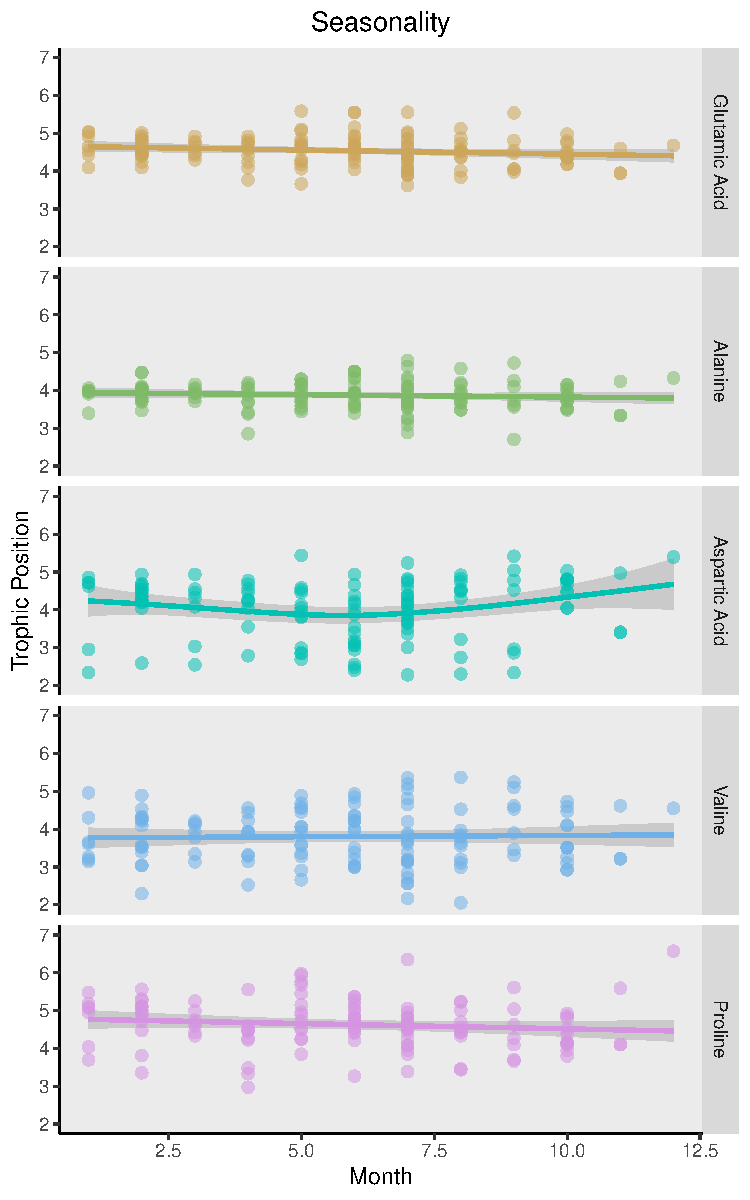
\includegraphics[width=0.55\textwidth]{figure/Ch3/FigureS1.pdf}
  \caption{Seasonality of harbor seal trophic position}
  \label{fig:season}
\end{figure}
\clearpage
\begin{landscape}
Figure 3.6: Time series of residuals by year for the three ocean condition models (physiological delay, 1-year ecological delay, 2-year ecological delay) with the most support for the four different trophic amino acids used in the models (glutamic acid, alanine, valine, and proline) with trophic position calculated using the source amino acid phenylalanine. Color corresponds to trophic amino acid, line shows the fit of a generalized additive model with a smoothed term by year and a k of 6. * denotes a significant smoothed term.
\newline 
\begin{figure}[h]
\centering
  \includegraphics[width=0.95\textwidth]{figure/Ch3/FigureS7.pdf}
  \caption{Temporal trends in ocean condition model residuals}
  \label{fig:ocresid}
\end{figure}
\end{landscape}
\clearpage
\begin{landscape}
Figure 3.7: Time series of residuals by year for the three food web models (physiological delay, 1-year ecological delay, 2-year ecological delay) with the most support for the four different trophic amino acids used in the models (glutamic acid, alanine, valine, and proline) with trophic position calculated using the source amino acid phenylalanine. Color corresponds to trophic amino acid, line shows the fit of a generalized additive model with a smoothed term by year and a k of 6. * denotes a significant smoothed term.
\newline 
\begin{figure}[h]
\centering
  \includegraphics[width=0.95\textwidth]{figure/Ch3/FigureS8.pdf}
  \caption{Temporal trends in prey availability model residuals}
  \label{fig:prresid}
\end{figure}
\end{landscape}
\clearpage

\textbf{Figure} \ref{fig:coefsmodel}: Coefficient estimates (dots) for
the best ocean condition (a-c) and prey availability (d-f) hierarchical
models with 95\% confidence intervals (whiskers). Y-axis labels describe
each covariate for supported models (\(\Delta AIC_c\) \textless{} 2) and
x-axis is the coefficient estimate for each covariate (magnitude of
trophic level change in response to the covariate). Colors correspond to
the temporal lags applied to the 2-year ecological delay models (pink, a
and f), 1-year ecological delay models (blue, b and e) and physiological
delay models (green, c and d). \newline 
\begin{figure}[h]
\centering
  \includegraphics[width=0.99\textwidth]{figure/Ch3/Figure2.pdf}
  \caption{Coefficients of harbor seal trophic position models}
  \label{fig:coefsmodel}
\end{figure}
\clearpage

\textbf{Figure} \ref{fig:conceptual}: Conceptual diagram interpreting
the mechanism of trophic position response (d) to estimated model
coefficients (Fig. 2d-f) included in the best food web models
(\(\Delta AIC_c\) \textless{} 2) for the 2-year ecological delay models
(a, pink arrows), 1-year ecological delay models (b, blue arrows) and
the physiological delay models (c, green arrows). Solid arrows indicate
indirect effects of covariates on harbor seal trophic position, signs
indicate the direction of trophic position response based on coefficient
estimates, and dashed arrows conceptually represent the mechanism
directly impacting harbor seal trophic position. \newline 
\begin{figure}[h]
\centering
  \includegraphics[width=0.9\textwidth]{figure/Ch3/Figure3.pdf}
  \caption{Conceptual representation of trophic position response to prey}
  \label{fig:conceptual}
\end{figure}
\clearpage

\textbf{Figure} \ref{fig:nbeta}: Distributions (density of probability,
y-axis) of calculated trophic position (x-axis) for harbor seals in this
study. Parameter values are described in Table \ref{tab:tpparam}. Colors
correspond to trophic amino acids (\emph{Tr}) and the grey box
represents ecologically realistic trophic positions for harbor seals if
they were to predate 1 trophic position above herring (trophic position
of 2.5, minimum expected value) and one trophic position below killer
whales (trophic position of 6, maximum). The value within the grey box
corresponds to the percentage of observed trophic position values that
fell within the ecologically realistic range. \newline 
\begin{figure}[h]
\centering
  \includegraphics[width=0.7\textwidth]{figure/Ch3/FigureS2.pdf}
  \caption{Trophic position estimates applying $\beta_{(i-o),N}$}
  \label{fig:nbeta}
\end{figure}
\clearpage

\textbf{Figure} \ref{fig:nvbeta}: Distributions (density of probability,
y-axis) of calculated trophic position (x-axis) for harbor seals in this
study applying four trophic position equation parameterizations and
\(\beta_{(i-o),NV}\) instead of \(\beta_{(i-o),N}\). \newline 
\begin{figure}[h]
\centering
  \includegraphics[width=0.8\textwidth]{figure/Ch3/FigureS3.pdf}
  \caption{Trophic position estimates applying $\beta_{(i-o),NV}$}
  \label{fig:nvbeta}
\end{figure}
\clearpage

\chapter{Recent divergent changes in Alaskan pinniped trophic position
detected using compound-specific stable isotope
analysis}\label{recent-divergent-changes-in-alaskan-pinniped-trophic-position-detected-using-compound-specific-stable-isotope-analysis}

\section{Abstract}\label{abstract-3}

Over the past century Alaskan pinnipeds have experienced dramatic
changes in abundance, but these changes have been highly variable across
species and region. In recent decades, changes in atmospheric forcing
and sea surface temperature have been particularly pronounced in the
Gulf of Alaska and eastern Bering Sea, impacting the food webs in which
Alaskan pinnipeds forage. We used compound-specific stable isotope
analysis of nitrogen in amino acids to estimate historic and modern
trophic position of harbor seals and Steller sea lions in the Gulf of
Alaska and Bristol Bay. We applied a Bayesian hierarchical framework to
determine whether shared trends through time exist across pinnipeds
(classified by species and region) on decadal scales. Model results
identified both shared trends through time and classification-specific
decadal changes in pinniped trophic position. The largest change in
trophic position occurred in the 2000s and 2010s and was observed in
both Steller sea lions and harbor seals in the Gulf of Alaska, but not
harbor seals in Bristol Bay or Iliamna Lake. Divergent trophic position
patterns in the 2000s were identified in the western stock of Steller
sea lions, which increased in trophic position, and sympatric harbor
seals in the northern Gulf of Alaska, which decreased in trophic
position. Our results indicate that these species have begun exploiting
distinct trophic niches or experiencing unique food web conditions in
recent decades in the Gulf of Alaska, likely in response to recent
climate-induced ecological change in the region.

\section{Introduction}\label{introduction-4}

Over the past century, pinniped populations in the northeast Pacific
Ocean have experienced changes in adult and pup abundances (Muto et al.,
\protect\hyperlink{ref-Muto2020}{2020}). Understanding specific drivers
of these population trends is important for management, as multiple
stocks have been listed as threatened or endangered over the past two
decades (Muto et al., \protect\hyperlink{ref-Muto2020}{2020}). The
observed population dynamics have also corresponded with shifts in both
the physical and ecological marine environment, which frequently occur
simultaneously. As a result, disentangling drivers of population trends
is complex, as multiple factors (environmental conditions, prey
availability, anthropogenic disturbances) can change in tandem and
potentially act synergistically on pinniped populations.

Data on long-term trends in trophic position across regions, species,
and populations is one potential way to assess how food web changes have
impacted pinnipeds in Alaska. This approach can identify how broad
shifts in foraging ecology correspond to changes in abundance and
population dynamics. More specifically, examining trophic position
during periods of declining versus increasing predator abundance can
provide insight into whether foraging behavior and prey availability are
important drivers of population dynamics. In this study, we aim to
identify whether common temporal trends in trophic ecology exist across
harbor seals (\emph{Phoca vitulina}) and Steller sea lions
(\emph{Eumetopias jubatus}) and their locations by deriving 70-years of
trophic position data from compound-specific stable isotope analysis
(CSIA) of museum specimens.

Following climatic changes in the 1970s that altered ocean currents and
sea surface temperature (Hare \& Mantua,
\protect\hyperlink{ref-Hare2000}{2000}), most Gulf of Alaska and Bering
Sea pinniped populations experienced declines that persisted through the
1990s (Muto et al., \protect\hyperlink{ref-Muto2020}{2020}). However,
these responses differed across populations and species. For example,
the western stock of Steller sea lions (located west of 144°W) decreased
from approximately 240,000 animals in the late 1970s to 50,000 in 2000
(Burkanov \& Loughlin, \protect\hyperlink{ref-Burkanov2005}{2005}).
Similarly, harbor seal populations in Prince William Sound and Glacier
Bay declined by approximately 60\% between the 1980s and 2000 (K. J.
Frost, Lowry, \& Ver Hoef, \protect\hyperlink{ref-Frost1999}{1999};
Womble et al., \protect\hyperlink{ref-Womble2010}{2010}). In contrast,
the eastern stock of Steller sea lions (located east of 144°W) increased
by 3-4\% per year over the same time period (Figure 4.2) (Muto et al.,
\protect\hyperlink{ref-Muto2020}{2020}; K. W. Pitcher et al.,
\protect\hyperlink{ref-Pitcher2007}{2007}). More recently, atmospheric
circulation anomalies in the northeast Pacific Ocean have resulted in
unprecedently warm sea surface temperatures during the past decade
(Walsh et al., \protect\hyperlink{ref-Walsh2018}{2018}) and this
environmental shift has altered fish abundances (N. A. Bond et al.,
\protect\hyperlink{ref-Bond2015}{2015}; Litzow et al.,
\protect\hyperlink{ref-Litzow2020}{2020}). For example, the
unprecedented marine heatwave that occurred in 2014 - 2016 triggered
dramatic ecosystem change, including a 71\% decline in Pacific cod in
the Gulf of Alaska (Barbeaux et al.,
\protect\hyperlink{ref-Barbeaux2020}{2020}). Declines in phytoplankton
biomass, forage fish abundance, and changes in community structure as a
whole were also observed (Suryan et al.,
\protect\hyperlink{ref-Suryan2021}{2021}). During this recent period of
environmental change, many pinniped populations have experienced
increases or stabilization of population abundance (Muto et al.,
\protect\hyperlink{ref-Muto2020}{2020}) (Figure 4.2), although declines
in some Gulf of Alaska Steller sea lion populations were observed
following the marine heat wave (Suryan et al.,
\protect\hyperlink{ref-Suryan2021}{2021}).

These variable changes in Alaskan pinniped populations over the past 50
years cannot be attributed to a single cause, as multiple environmental,
anthropogenic, and ecological factors have changed simultaneously. For
example, the rapid decline of the western stock of Steller sea lions
between the 1970s and 1990s has been attributed to myriad factors,
including change to the physical environment, competition with fisheries
for common prey, predation, disease, and human-caused mortality (S.
Atkinson, Demaster, \& Calkins,
\protect\hyperlink{ref-Atkinson2008}{2008}). Glacier Bay harbor seal
populations have primarily, but not exclusively, been impacted by the
decline of sea ice, which provides a majority of their haulout sites
(Womble et al., \protect\hyperlink{ref-Womble2010}{2010}). Population
declines have also been associated with increased numbers of tour
vessels, particularly in glacier fjords that provide important nursing
and whelping habitat (Jansen, Boveng, Ver Hoef, Dahle, \& Bengtson,
\protect\hyperlink{ref-Jansen2015}{2015}; Mathews et al.,
\protect\hyperlink{ref-Mathews2016}{2016}). The differences in pinniped
population trends across the Gulf of Alaska and Bering Sea suggest
varied environmental and ecological drivers underlying these dynamics.
Interestingly, harbor seals and Steller sea lions that occur in the same
geographic region (sympatric) have experienced different population
trends over similar time period (Figure 4.2). Identifying trophic
position trends through time that are shared, compared to changes that
only impact a specific species or region, can elucidate how widescale
ecological forcing versus localized change influence top predators and
potentially explain variable population abundance trends.

Both harbor seals and Steller sea lions exhibit generalist, piscivorous
foraging strategies, although differences in foraging range, body size,
and diet exist. Adult harbor seals have high site fidelity,
opportunistically forage 5 - 10 km from haulout sites and at depths
\textless{} 200 m (M. M. Lance et al.,
\protect\hyperlink{ref-Lance2012}{2012}; Lowry, Frost, Ver Hoep, \&
Delong, \protect\hyperlink{ref-Lowry2001}{2001}), and weigh up to 300
pounds. Steller sea lions are central place foragers known to migrate to
prey aggregations on the continental shelf and oceanographic boundary
zones (E. H. Sinclair \& Zeppelin,
\protect\hyperlink{ref-Sinclair2002}{2002}; Womble \& Sigler,
\protect\hyperlink{ref-Womble2006}{2006}). Foraging trips can last 1-3
days (Maniscalco, Parker, \& Atkinson,
\protect\hyperlink{ref-Maniscalco2006}{2006}) with average distances of
133 km for adult females (Merrick \& Loughlin,
\protect\hyperlink{ref-Merrick1997}{1997}), although foraging trips are
shorter in the breeding season (Maniscalco et al.,
\protect\hyperlink{ref-Maniscalco2006}{2006}). Adult females can weigh
up to 800 pounds whereas adult males can exceed 2,500 pounds, indicating
a higher energetic demand compared to harbor seals. Diet studies of
Steller sea lions and harbor seals are spatially and temporally limited,
and primarily utilize scat samples. In the Gulf of Alaska, gadids,
cephalopods, and forage fishes are prevalent in both harbor seal and
Steller sea lion diet (Geiger et al.,
\protect\hyperlink{ref-Geiger2013}{2013}; E. H. Sinclair \& Zeppelin,
\protect\hyperlink{ref-Sinclair2002}{2002}), whereas salmonids are also
important for harbors seals in Bristol Bay and Iliamna lake (Hauser,
Allen, Rich, \& Quinn, \protect\hyperlink{ref-Hauser2008}{2008}).

Stable isotopes have been used to reconstruct historical differences in
diet and trophic position in Alaskan pinnipeds (Brennan et al.,
\protect\hyperlink{ref-Brennan2019}{2019}; Hirons, Schell, \& Finney,
\protect\hyperlink{ref-Hirons2001}{2001}; Keith A. Hobson, Sease,
Merrick, \& Piatt, \protect\hyperlink{ref-Hobson1997}{1997}). These
previous studies utilized bulk stable isotope analysis exclusively and
were therefore limited in their inferential strength. Differences in the
bulk \textsuperscript{15}N/\textsuperscript{14}N of consumer tissues can
indicate either a trophic level change of the consumer or a change in
nitrogen resources at the base of the food web. The specific cause of
the isotopic variation cannot be ascertained from consumer bulk stable
isotope values unless the data are paired with temporal information on
\textsuperscript{15}N/\textsuperscript{14}N in primary producers. Lack
of consistent, concurrent sampling of nitrogen stable isotope
composition of primary producers therefore presents a challenge for
previous long-term studies of the trophic dynamics of consumers from
bulk stable isotope data. CSIA data address this challenge, as amino
acids exhibit two distinct patterns in isotopic enrichment: trophic
amino acids (i.e., glutamic acid, alanine, proline) become enriched in
\textsuperscript{15}N with each trophic transfer and source amino acids
(i.e., phenylalanine) show minimal change and thus are reflective of the
base of the food web (Chikaraishi et al.,
\protect\hyperlink{ref-Chikaraishi2009}{2009}; McClelland \& Montoya,
\protect\hyperlink{ref-McClelland2002}{2002}; N. Ohkouchi et al.,
\protect\hyperlink{ref-Ohkouchi2017}{2017}). With the ability to
internally correct for expected changes in
\textsuperscript{15}N/\textsuperscript{14}N at the base of the food web
{[}Feddern et al. (\protect\hyperlink{ref-Feddern2021}{2021}); Ramirez
et al. 2021{]}, CSIA allows for a more robust retrospective analysis of
consumer trophic dynamics on decadal and century scales.

The objective of this work is to describe and compare changes in trophic
ecology for Alaskan pinnipeds throughout the past century and
investigate trophic position differences for sympatric populations. We
apply hierarchical Bayesian analyses to 70 years of trophic position
data derived from CSIA from pinnipeds (harbor seal and Steller sea lion)
in the Gulf of Alaska, Bristol Bay, and a small population of freshwater
harbor seals in Iliamna Lake, Alaska which is adjacent to Bristol Bay.
We build on previous research examining pinniped nitrogen stable isotope
composition (Brennan et al., \protect\hyperlink{ref-Brennan2019}{2019};
Hirons et al., \protect\hyperlink{ref-Hirons2001}{2001}; Keith A. Hobson
et al., \protect\hyperlink{ref-Hobson1997}{1997}; Misarti et al.,
\protect\hyperlink{ref-Misarti2009}{2009}) by adding two decades of data
to the record (2000s and 2010s) and incorporating a broad spatial scope
(Bristol Bay, Iliamna Lake, Gulf of Alaska). Additionally, by analyzing
nitrogen stable isotopes derived from amino acids, we were able to
control for known changes in nitrogen resources and phytoplankton
composition at the base of the food web that can confound trophic
position interpretations from bulk stable isotope data collected over
decadal scales (Feddern et al.,
\protect\hyperlink{ref-Feddern2021}{2021}). Furthermore, by comparing
trophic position dynamics across species and region through time,
regional and location-specific ecological responses to a changing
ecosystem can be identified.

\section{Methods}\label{methods-3}

\subsection{Sample collection and
analysis}\label{sample-collection-and-analysis-2}

Samples were obtained using methods described in Feddern et al.
(\protect\hyperlink{ref-Feddern2021}{2021}). Briefly, harbor seal and
Steller sea lion bones were sampled from specimens curated at the
University of Alaska Museum of the North (Supplementary Information
Table S1). Specimens were treated by maceration in warm water and soaked
in a dilute ammonia solution then stored in acid free boxes. Adult
specimens were sampled exclusively to avoid dietary differences between
adults and juveniles. Specimens were classified based on species and
region. We prioritized long-term temporal coverage in four regional
classifications of harbor seals (Iliamna Lake, southeast Gulf of Alaska,
northern Gulf of Alaska, eastern Bering Sea) and two regional
classifications of Steller sea lions (eastern and western stocks) for a
total of 6 species x region classifications. Specimens were extremely
limited for the eastern Steller sea lion stock (n = 2) and Iliamna Lake
harbor seas (n = 3). We also prioritized specimens with sex and age
identifications, but these data were not available for some specimens. A
total of 106 harbor seal and 21 Steller sea lion specimens were sampled
representing the 1950s to 2010s (Figure \ref{fig:map4} ).

Steller sea lions were classified according to the National Oceanic and
Atmospheric Administration's (NOAA) distinct population segments, where
Steller sea lions east of 144°W are considered the eastern stock and
west of 144°W are considered the western stock (Figure \ref{fig:map4} ).
NOAA has identified twelve stocks of harbor seals in Alaska and, due to
limitations of archived specimens, harbor seals were not able to be
classified according to NOAA stocks. Instead, they were classified based
on their range relative to the Steller sea lion stocks and utilization
of marine versus freshwater habitats. Harbor seals that were west of
144°W, which included samples from the Prince William Sound and Cook
Inlet/Shelikof Strait stocks (Figure \ref{fig:map4} ), were classified
as northern Gulf of Alaska harbor seals. Harbor seals that were located
east of 144°W, which included samples from the Glacier Bay/Icy Strait,
Sitka/Chatham Strait, Lynn Canal/Stephens Passage, Dixon/Capes
Decisions, and Clarence Strait stocks (Figure \ref{fig:map4} ), were
classified as southeast Gulf of Alaska harbor seals. The Bristol Bay
harbor seal stock was divided into two classifications, Bristol Bay
referring to marine harbor seals, and Iliamna Lake referring to
freshwater harbor seals (Figure \ref{fig:map4} ). This allowed for
comparison of three pairs of geographically overlapping classifications:
western stock of Steller sea lions and northern Gulf of Alaska harbors
seals, eastern stock of Steller sea lions and southeast Gulf of Alaska
harbor seals, and Bristol Bay and Iliamna Lake harbor seals.

\subsection{Trophic position
calculation}\label{trophic-position-calculation}

Bone collagen within the samples was decalcified, acid hydrolyzed,
derivatized and analyzed for compound-specific stable isotope analysis
(CSIA) of nitrogen (\(\delta^{15}N\)) for 12 individual amino acids
following the protocol described in Feddern et al.
(\protect\hyperlink{ref-Feddern2021}{2021}). \(\delta^{15}N\) was
measured as:
\begin{equation} 
  \delta^{15}N ( \textperthousand vs. air) =   
  [(\frac{^{15}N/^{14}N_{Sample}}{^{15}N/^{14}N_{Air}} -1)*1000]
  \label{eq:deltN2}
\end{equation}
Collagen samples were measured in triplicate with a laboratory standard
containing a 12 amino acid mixture of known isotopic composition. Full
analytical details are described in Appendix S1.

Trophic position was calculated using a harbor seal-specific trophic
discrimination factor (difference in
\textsuperscript{15}N/\textsuperscript{14}N between trophic and source
amino acids in consumers for a trophic transfer; Germain et al.
(\protect\hyperlink{ref-Germain2013}{2013})). This approach assumed
trophic discrimination factors (TDF) derived from controlled feeding
studies of harbor seals were similar to Steller sea lions. Applying a
``multi-TDF'' approach that combines both average and taxa-specific TDF
can improve trophic position estimates in marine predators including
pinnipeds (Germain et al., \protect\hyperlink{ref-Germain2013}{2013};
McMahon et al., \protect\hyperlink{ref-McMahon2019}{2019}). The
following equation was used to determine the trophic position of each
sampled individual:
\begin{equation} 
Trophic Position =   
  \frac{\delta^{15}N_i - \delta^{15}N_o - TDF_{(i-o),j} - \overline{\beta}_{(i-o)}}{\overline{TDF}_{(i-o)}}+2
  \label{eq:TP}
\end{equation}
where, \(\delta^{15}N_i\) is the measured stable isotope composition of
a trophic amino acid i in a sample and \(\delta^{15}N_o\) is the stable
isotope composition of a source amino acid o in a sample.
\(\overline{TDF}_{(i-o)}\) is the mean difference between given trophic
amino acid \emph{i} and source amino acid \emph{o} across all consumers
described in J. M. Nielsen et al.
(\protect\hyperlink{ref-Nielsen2015}{2015}). \(TDF_{(i-o), j}\) is the
trophic discrimination factor between trophic amino acid \emph{i} and
source amino acid \emph{o} from a controlled feeding study of a specific
consumer \emph{j}; here we use harbor seals from Germain et al.
(\protect\hyperlink{ref-Germain2013}{2013}) (Table \ref{tab:paramval}).
\(\overline\beta_{(i-o)}\) is the mean difference in \(\delta^{15}N\)
across aquatic phytoplankton between a specific trophic amino acid
\emph{i} and source amino acid \emph{o} {[}J. M. Nielsen et al.
(\protect\hyperlink{ref-Nielsen2015}{2015}); Table
\ref{tab:paramval}{]}. J. M. Nielsen et al.
(\protect\hyperlink{ref-Nielsen2015}{2015}) also determined using
multiple amino acids to estimate trophic position improves precision.
Therefore, we used multiple trophic amino acids \emph{i} (alanine,
glutamic acid, aspartic acid and proline) and one source amino acid
\emph{o} (phenyalanine) to calculate trophic position (Table
\ref{tab:paramval}). These amino acids were chosen based on their
prevalence in previous studies to derive parameters for equation 2, and
their concentrations in bone collagen (see Appendix S1).

\subsection{Model framework}\label{model-framework}

Sex was considered as a predictor for trophic position, however, sex
metadata were not available for all specimens. In order to evaluate
difference in trophic position by sex, we fit linear statistical models
to each individual trophic amino acid, by classification (species x
region). These models took the following form:
\begin{equation} 
y_i = \alpha + \boldsymbol\beta x_i + \epsilon_i, \epsilon \sim N(0,\sigma)
  \label{eq:linsex}
\end{equation}
where, \(y_i\) is trophic position for an individual amino acid and
\(\boldsymbol\beta\) is a vector of coefficients for the predictor, in
this case sex, and \(\epsilon\) are residual errors assumed to be
normally distributed with mean 0 and standard deviation \(\sigma\).
There was not sufficient metadata for the eastern stock Steller sea lion
population or the Iliamna Lake population and these two classifications
were omitted from this analysis.

A Bayesian hierarchical mixed effects model was used to identify decadal
change across pinniped classifications (species x region), and the
degree to which these changes were shared by testing the effects of
classification, decade, and a classification-decade interaction as
either population-level (fixed) or group-level (random) effects (see
candidate models in Table \ref{tab:paramval}). Hierarchical models share
information across `groups' to identify common responses, which refers
to both decade and classification in this study. The interaction term
allows for increased flexibility, letting each classification have
slight departures from the group-level means. The mean and variance of
pinniped trophic position for each region-species classification and
decade were estimated using a generalized linear Bayesian hierarchical
model with decade, population, and trophic amino acid as predictors:
\begin{equation} 
y_i = \boldsymbol\alpha + \boldsymbol\beta x_i + \epsilon_i, \epsilon \sim N(0,\sigma_y)
  \label{eq:linsex}
\end{equation}
\begin{equation} 
\boldsymbol\alpha_{k=1:k} \sim N(\mu_{\alpha,k},\sigma_{\alpha,k})
  \label{eq:linsex}
\end{equation}
where, for data point \emph{i}, \(\boldsymbol\beta\) is a vector of
coefficients for the unpooled predictors (fixed effects, Table
\ref{tab:paramval}) and \(\boldsymbol\alpha\) is a vector of
coefficients for the partially pooled group-level predictors (random
effects, Table \ref{tab:paramval}) for group \emph{k} (amino acid,
decade or classification). At minimum, the \(\boldsymbol\alpha\)
included a random term for the amino acid corresponding to data point
\emph{i}, and depending on the model included up to a total of 4 random
effects (also effects of decade, classification, and their interaction,
Model 6 in Table \ref{tab:paramval}). For each random effect included,
\(\mu_{α,k}\) and \(\sigma_{α,k}\) are hyperparameters representing the
mean and standard deviation of group-level effects on trophic position,
for random effect \emph{k}. For models with more than one random effect,
we assumed the deviations to be independent and uncorrelated. We
considered models that included decade, classification, and the
interaction between decade and classification either as fixed or random
effects (e.g.~Model 4 v Model 6, Table \ref{tab:paramval}), but did not
consider models that included both as fixed and random (Table
\ref{tab:paramval}). Parameter estimates were obtained using the brms
package (Burkner et al. 2017, version 2.14.4) in R (R Core Development
Team 2021, version 3.6.2), which implements a Hamiltonian Monte Carlo
sampler and its extension no-U-turn sampler (Hoffman and Gelman 2014)
through Stan (Stan Development Team 2020). Minimally informative priors
were used for random effects (normal distributions with a mean of 0 and
variance of 10) and fixed effects (Student's t-distribution with a mean
of 0, standard deviation of 2.5 and 3 degrees of freedom). Trophic amino
acid was included as a random effect for all models (Table
\ref{tab:paramval}). Selection of the best models (Table
\ref{tab:paramval}) given the data was based on approximate
leave-one-out cross-validation (LOOIC) using the loo package (Veharti et
al. 2017, version 2.4.1).

\section{Results}\label{results-3}

We found no differences between the average male and female pinniped
trophic position over the 50-year study period (Figure \ref{fig:sex4} )
for the four tested species-region classifications. This finding was
consistent for all trophic amino acids-source amino acid pairs (Figure
\ref{fig:sex4} ). Based on glutamic acid trophic position estimates,
both western stock Steller sea lions (2.6 ± 0.5; mean ± sd) and eastern
stock Steller sea lions (2.7 ± 0.16) had similar trophic positions.
Harbor seals in the Gulf of Alaska foraged higher in the food web than
their Steller sea lion counterparts (Figure \ref{fig:sex4} ). Harbor
seals in the southeast region had a higher trophic position on average
than any other pinniped in this study (3.5 ± 0.3) but were similar to
harbor seals in the northern region (3.3 ± 0.5). Bristol Bay (3.1 ± 0.4)
and Iliamna lake (3.0 ± 0.3) harbor seals had a lower trophic position
than their Gulf of Alaska counterparts on average (Figure \ref{fig:sex4}
).

\subsection{Common trends in Alaskan pinniped trophic
position}\label{common-trends-in-alaskan-pinniped-trophic-position}

The best performing model (Table \ref{tab:paramval}, model 6) of
pinniped trophic position included both species-region classification
and decade as random effects (shared trends) along with an interaction
between population and decade (Table \ref{tab:paramval}). Based on the
support for decade and classification to be included as group-level
effects, these data support consistent differences between
classifications over time, as well as differences between trophic
position for all classifications. The supported interaction between
population and decade (Table \ref{tab:paramval}) indicates distinct
decadal changes in trophic position for species-region classifications
exist. The model that included decade, classification, and the
interaction between decade and classification as fixed effects (model 4)
was also supported based on the models LOOIC (Table \ref{tab:paramval}).
Therefore, the inclusion of the interaction term was more important for
improving model performance than inclusion of decade and classification
as fixed versus random effects.

There were consistent differences in trophic position that varied by
species and ocean basin for the model with the most support. Harbor
seals in the Gulf of Alaska had higher trophic position than their
Steller sea lion counterparts. The mean difference of the posterior
distributions indicated southeast Gulf of Alaska harbor seals have
historically fed at 0.32 {[}-0.01, 0.61{]} (highest density 80\%
credible interval) trophic levels higher than sympatric eastern stock
Steller sea lions (Figure \ref{fig:region} ). Similarly, the mean
difference of posterior distributions showed northern Gulf of Alaska
harbor seals fed 0.28 {[}-0.03, 0.50{]} trophic levels higher than the
sympatric western stock Steller sea lions. Within the Gulf of Alaska,
the posterior distributions for trophic position overlapped 39\% between
harbor seals and Steller sea lions in both the eastern and western
regions (Figure \ref{fig:region} ). Iliamna Lake harbor seals have
historically fed at a lower trophic level (mean posterior difference
0.16 {[}-0.11, 0.41{]}) than harbor seals in Bristol Bay, but these two
classifications have 66\% overlap of the group-level posterior
distributions for trophic position (Figure \ref{fig:region} ). The 80\%
credible intervals included 0 for most region-species classifications
thus the posterior probabilities support marginal evidence for
consistent differences in trophic position between classifications.
Regardless, the differences in posterior means were large, although the
distributions were wide.

There were no consistent decadal differences in trophic position across
the region-species classification (Figure \ref{fig:decade} ). Pinniped
trophic position in the 2000s was slightly higher for all
classifications (mean posterior difference 0.03 {[}-0.09, 0.16{]}) on
average compared to 1990 and the posterior distributions for 1990 and
2000 had an 85\% overlap (Figure \ref{fig:decade} ). Similarly,
posterior distributions in between 2000 and 2010 had a mean difference
of -0.1 {[}-0.27, 0.08{]} with a 65\% overlap (Figure \ref{fig:region}
). Overall, decadal differences in pinniped trophic position through
time were smaller than the region-species classification effects and
were likely ecologically inconsequential.

\subsection{Spatial and temporal differences in pinniped trophic
structure}\label{spatial-and-temporal-differences-in-pinniped-trophic-structure}

Distinct decadal changes in trophic position were observed for each
species-region classification and varied more than the shared decadal
changes (Figure \ref{fig:full} ) as indicated by the
decade-classification interaction. Most, but not all, pinniped
classifications experienced substantial trophic level change in 2000 or
2010 but the magnitude and direction of this change varied by
region-species classification based on the combined effects of decade,
classification, and the decade-classification interaction (Figure
\ref{fig:full} ). The recent decadal change in trophic position was most
prominent for the western stock of Steller sea lions which had a mean
trophic level decrease of 0.43 {[}-0.25, -0.60{]} from 1990 to 2000 (a
percent decrease of 0.15) with only a 21\% overlap between the posterior
distributions (Figure \ref{fig:full} E). This decline in trophic
position remained in the 2010s. A similar decline was observed in the
southeast Gulf of Alaska harbor seals. This population experienced
relatively stable trophic position from 1960-1990, which then declined
on average by 0.31 {[}-0.19, -0.45{]} trophic levels in 2000 (33\%
posterior overlap) (Figure \ref{fig:full} C). In contrast, harbor seals
in the northern Gulf of Alaska had variable trophic position across
decades and had the highest trophic position in 2000 in contrast to
their southeast Gulf of Alaska harbor seals and Steller sea lion
counterparts (Figure \ref{fig:full} B). Data were only available for
2000 and 2010 for the eastern stock Steller sea lions, and trophic
position was similar for this population during both of these decades
(Figure \ref{fig:full} F). Both Bristol Bay and Iliamna Lake harbor
seals had relatively stable trophic position from 1950s until 2010s
(Figure \ref{fig:full} A \& B). Bristol Bay harbor seals experienced
their lowest trophic level in the 1990s with a 0.24 {[}-0.54, 0.00{]}
trophic level decrease compared to the 1970s and 2000s, but the
posterior distribution still overlapped 54\% with other decades (Figure
\ref{fig:full} A).

\section{Discussion}\label{discussion-3}

Over the past 70 years, Alaskan pinnipeds have exhibited both common and
distinct differences in trophic position across region-species
classification on decadal scales (Table \ref{tab:paramval}). While
potential drivers of change in trophic position were not tested in this
study due to data limitations, our results support a combination of
local-scale (i.e., vessel traffic, reduction of glacial ice, local
foraging) and regional-scale (i.e., environmental condition, basin-wide
prey abundance) changes may be influencing pinniped trophic ecology.
Furthermore, the largest decadal changes in pinniped trophic position
were distinct for each region-species classification and were most
apparent during the most recent two decades (2000s and 2010s). These
patterns are more pronounced in the Gulf of Alaska compared to Bristol
Bay (Figures 5 \& 6).

\subsection{Regional and species trends in harbor seal trophic
position}\label{regional-and-species-trends-in-harbor-seal-trophic-position}

Both Steller sea lions and harbor seals exhibit generalist foraging
patterns (Geiger et al., \protect\hyperlink{ref-Geiger2013}{2013}; M. M.
Lance et al., \protect\hyperlink{ref-Lance2012}{2012}). Diets of Alaskan
pinnipeds consist of similar prey species but vary between species,
population, and local availability of prey (Hirons et al.,
\protect\hyperlink{ref-Hirons2001}{2001}; Iverson, Frost, \& Lowry,
\protect\hyperlink{ref-Iverson1997}{1997}). Bulk stable isotope studies
in the Gulf of Alaska have shown that Steller sea lions feed lower in
the food web compared to harbor seals (Iverson et al.,
\protect\hyperlink{ref-Iverson1997}{1997}). Our CSIA analysis confirms
the interpretation of these previous studies that isotopic differences
can be attributed to trophic position changes and not isotopic shift of
basal phytoplankton resources. Both western and eastern stock Steller
sea lions have lower trophic position compared to sympatric harbor seal
populations but have similar trophic position compared to other
populations such as Iliamna Lake. However, despite known differences in
both diet (Geiger et al., \protect\hyperlink{ref-Geiger2013}{2013}; E.
H. Sinclair \& Zeppelin, \protect\hyperlink{ref-Sinclair2002}{2002}) and
nearshore versus offshore foraging (Lowry et al.,
\protect\hyperlink{ref-Lowry2001}{2001}; Merrick \& Loughlin,
\protect\hyperlink{ref-Merrick1997}{1997}) between the two species, our
results also show historical overlap in trophic position, indicating
potential trophic redundancy between harbor seals and Steller sea lions
in the Gulf of Alaska.

Harbor seals in Bristol Bay and Iliamna Lake are managed as a single
population (Muto et al., \protect\hyperlink{ref-Muto2020}{2020}) despite
lack of evidence of migration by the freshwater population and
utilization of different resources (Brennan et al.,
\protect\hyperlink{ref-Brennan2019}{2019}). A previous study of
strontium and carbon stable isotopes showed Iliamna Lake harbor seals
utilize freshwater-derived resources (resident lake fishes),
particularly early in life, and exhibit an ontogenetic shift to more
marine resources (returning sockeye salmon) later in life (Brennan et
al., \protect\hyperlink{ref-Brennan2019}{2019}). Based on CSIA nitrogen
data, Iliamna Lake harbor seals also forage lower in the food web
compared to Bristol Bay harbor seals. In addition, both classifications
exhibited trophic stability, with the Bristol Bay harbor seals only
experiencing a trophic shift in the 1990s relative to the 1960s and
1970s. This coincided with the lowest sockeye salmon returns to Iliamna
Lake on record (Hilborn, Quinn, Schindler, \& Rogers,
\protect\hyperlink{ref-Hilborn2003}{2003}). Interestingly, the decrease
in trophic position in the 1990s occurred simultaneously with decreases
in basin wide Bristol Bay harbor seal abundance in the late 1990s, which
then stabilized and increased in the 2000s and 2010s (Figure 4.2). Data
were not available for the freshwater harbor seals between 1990 and 2000
and thus it is unclear whether the freshwater population also
experienced a trophic position change during the 1990s when sockeye
salmon returns were low. While quantitative comparisons to salmon
abundance were not made in this study, salmon population abundance and
harbor seal trophic ecology and population trends are seemingly
interrelated.

\subsection{Recent trophic position changes in the Gulf of
Alaska}\label{recent-trophic-position-changes-in-the-gulf-of-alaska}

Trophic position changes were observed in all pinniped classifications
in the Gulf of Alaska during the past two decades, although the
direction of these changes varied on more local scales. During the past
two decades (2000-2020), harbor seals in the Gulf of Alaska have
experienced stabilization of most monitored populations following
long-term declines that persisted from the 1950s through the 1990s
(Figure 4.2, Muto et al. (\protect\hyperlink{ref-Muto2020}{2020})).
During this same time period, harbor seals in both southeast and
northern Gulf of Alaska experienced a shift in trophic position that was
particularly prominent in the 2000s compared to historic estimates of
trophic position (Figure \ref{fig:full} B \& C). It is possible that the
observed trophic position shift may have contributed to the population
stabilization of Gulf of Alaska harbor seals, either by an increase in
prey availability or opportunistically foraging on a novel prey source.
Gagne, Hyrenbach, Hagemann, \& Van Houtan
(\protect\hyperlink{ref-Gagne2018}{2018}) observed similar trophic
position declines in seabird populations, which were attributed to a
shift in diet from fish to squid. A similar dietary shift could explain
the observed trophic position shift in southeast Gulf of Alaska harbor
seals and western stock Steller sea lions.

Recent regional change in the Gulf of Alaskan food webs has been well
documented in other species and primarily attributed to bottom-up
effects of climate (Barbeaux et al.,
\protect\hyperlink{ref-Barbeaux2020}{2020}; Litzow et al.,
\protect\hyperlink{ref-Litzow2020}{2020}). These region-wide trends
likely altered prey availability for pinniped populations in the Gulf of
Alaska. How pinniped populations have adapted their foraging ecology,
however, indicates regional and species trophic divergence, which could
be attributed to either local-scale foraging adaptations or differences
in prey availability. Pinniped groups that overlap in space (Figure
\ref{fig:map4} ) revealed divergent trends in trophic position between
Steller sea lions and harbor seals in recent decades (Figure
\ref{fig:full} B \& E). For example, trophic position of northern Gulf
of Alaska harbor seals increased in the 2000s while the western stock of
Steller sea lions decreased. For western stock Steller sea lions, this
shift also persisted into the 2010s (Figure \ref{fig:full} E). Posterior
distributions of western stock Steller sea lions and northern Gulf of
Alaska harbor seals overlapped by 63\% in the 1950s but only overlapped
by 3\% in the 2000s (Figure \ref{fig:full} B \& E). The recent change in
pinniped trophic position within the Gulf of Alaska coincided with
population abundance stabilization, albeit at lower than historical
abundance for most populations. This trophic divergence indicates there
could be increased competition for resources between northern Gulf of
Alaska harbor seals and western stock Steller sea lions resulting in
diet adaptations. Similar comparisons were challenging to make for the
eastern stock of Steller sea lions and southeast Gulf of Alaska harbor
seals due to limitations in historical data for the former. However,
trophic position in the 2000s showed a 38\% overlap (Figure
\ref{fig:full} C \& E) between the two species, indicating any trophic
divergence between them may be less pronounced in this region, if
existent.

The observed divergent trends indicate differences in how Alaskan
pinnipeds are adapting to environmental and ecological changes. Trophic
position changes from stable isotope data can be accounted for by: 1)
prey switching between different species, 2) consuming different sizes
of the same prey, or 3) consuming different quality prey. These changes
can occur at the consumer level (pinnipeds) or lower in the food web and
still be reflected in consumer stable isotope signature and thus trophic
position. In recent decades, Pacific salmon and halibut in Alaska have
both declined in size (K. K. Holsman et al.,
\protect\hyperlink{ref-Holsman2019}{2019}; Oke et al.,
\protect\hyperlink{ref-Oke2020}{2020}). These changes in size
distributions of prey have been attributed to changes in marine mammal
populations (Groskreutz et al. 2019) and likely contributed to the
observed trophic position declines in western Steller sea lion and
southeast Gulf of Alaska harbor seals. In contrast, consuming
low-quality prey with lower protein content and greater amino acid
imbalance between consumer and prey increases the amino acid trophic
enrichment factor of nitrogen (McMahon et al.,
\protect\hyperlink{ref-McMahon2015}{2015}). If not accounted for in
trophic position equations, this increase in trophic enrichment factor
can result in erroneously high trophic position estimates. This may
explain the observed increase in estimated trophic position in northern
Gulf of Alaska harbor seals where this population may be consuming a
greater proportion of lower quality prey (i.e., crustaceans, shrimp,
cephalopods) in recent decades rather than feeding on prey species that
are higher in the food web.

\subsection{Considerations and limitations for CSIA
analyses}\label{considerations-and-limitations-for-csia-analyses}

The data in this study were limited in sample size primarily due to the
availability of archived specimens. As a result, we were not able to
discern between known fine scale differences in populations or annual
trends. For example, harbor seals in the southeast Gulf of Alaska
consist of 13 individual stocks. Due to limitations in the number of
archived specimens, these stocks were pooled and analyzed as a single
classification despite known differences in genetic structure (Muto et
al., \protect\hyperlink{ref-Muto2020}{2020}). Given the observed broad
range in trophic position of these generalist predators, it is unlikely
that inclusion of finer spatial dynamics would have changed the
supported model, although variation in temporal trends within a
classification may have been identified. Similarly, data were only
available for eastern stock Steller sea lions for 2000s and 2010s. As a
result, no historical comparisons were possible and the conclusions
about this population are tentative. Nonetheless, this dataset offers
historic documentation of pinniped trophic position that can be updated
with future samples or additional archived specimens.

Trophic position estimates in this study were low compared to known
foraging strategies of these pinnipeds. For example, Steller sea lions
eat primarily walleye pollock and Atka mackerel (Keith A. Hobson et al.,
\protect\hyperlink{ref-Hobson1997}{1997}; Trites, Calkins, \& Winship,
\protect\hyperlink{ref-Trites2007}{2007}), which would indicate a
trophic position of 3 or higher. Mean trophic position for Steller sea
lions was closer to 2.7 in this study, which is lower than expected
based on known foraging ecology. It is common for CSIA to underestimate
trophic position of marine predators (Germain et al.,
\protect\hyperlink{ref-Germain2013}{2013}; McMahon et al.,
\protect\hyperlink{ref-McMahon2019}{2019}) and the inclusion of multiple
amino acid pairs and a multi-trophic enrichment factor framework did not
fully resolve this issue. J. M. Nielsen et al.
(\protect\hyperlink{ref-Nielsen2015}{2015}) found trophic position
estimates can be highly sensitive to the applied \(\beta\) values in
equation 2. In our trophic position calculation, we assumed a constant
\(\beta\) represented by marine diatoms. However, \(\beta\) values
differ by more than 11 per mille between seagrasses and diatoms (H. B.
Vander Zanden et al., \protect\hyperlink{ref-VanderZanden2013}{2013})
which has been attributed to differences between vascular and
nonvascular plants (B. Choi et al.,
\protect\hyperlink{ref-Choi2017}{2017}, Ramirez et al. 2021). If
vascular plants, such as seagrasses, contribute to the food web in
addition to non-vascular algae, the applied β would be too high and
would result in underestimation of trophic position of marine consumers
(B. Choi et al., \protect\hyperlink{ref-Choi2017}{2017}, Ramirez et al.
2021). Even a 10\% contribution of vascular plant-derived nitrogen to
the food web would result in an underestimation of 0.2 trophic position.
It is likely that vascular plants at least partially contribute to the
Alaskan food web, as seagrass beds provide essential habitat and food
for many fish species and invertebrates. Consideration for variable
\(\beta\) values may be helpful in resolving trophic position
underestimation of future studies, especially in cases where consumer
carbon stable isotope data is available and contributions of seagrasses
to the food web are well documented.

\subsection{Conclusions and
Implications}\label{conclusions-and-implications}

Marine ecosystems in Alaska are experiencing unprecedented environmental
change that has altered abundance and size distributions of many fish
species consumed by pinnipeds (Barbeaux et al.,
\protect\hyperlink{ref-Barbeaux2020}{2020}; K. K. Holsman et al.,
\protect\hyperlink{ref-Holsman2019}{2019}; Oke et al.,
\protect\hyperlink{ref-Oke2020}{2020}; Suryan et al.,
\protect\hyperlink{ref-Suryan2021}{2021}). Heterogeneity in diet and
foraging locations allow top predators to adjust to availability of
resources by altering their foraging. Based on the observed
region-species specific changes in trophic position over the past two
decades, pinnipeds are experiencing different food web conditions than
in the past, even those that occur in similar geographic regions. This
may be the result of adapting foraging strategies to exploit other prey
resources or a change that is occurring lower in the food web and is
measurable in predators. While our results cannot discern between these
two mechanisms of trophic level change, we can conclude that recent food
web dynamics have impacted pinniped trophic ecology in Alaska. Future
responses of pinnipeds to food web change will likely be locally
variable between species, even those that occur within similar
geographic regions.

\clearpage

\section{Tables}\label{tables-3}

\textbf{Table} \ref{tab:paramval}: Parameter values for trophic
discrimination factors between a trophic amino acid (\emph{i}) and
phenylalanine (\emph{o}) for harbor seals (\(TDF_{(i-o), j}\)), for an
average consumer (TDF(i-o) ), and for primary producers
(\(\beta_{(i-o)}\)) derived from previous studies to apply a multi amino
acid framework to equation 2.

\begingroup\fontsize{8}{10}\selectfont
\begin{longtable}[t]{l>{\raggedright\arraybackslash}p{10em}>{\raggedright\arraybackslash}p{10em}>{\raggedright\arraybackslash}p{10em}}
\caption{\label{tab:paramval}Trophic position parameter values for Equation 2}\\
\toprule
Trophic Amino Acid (i) & $\overline{\beta}_{(i-o)}$ & $TDF_{(i-o),j}$ & $\overline{TDF}_{(i-o)}$\\
\midrule
Glutamic acid (Glu) & 2.9 & 3.4 & 6.6\\
Alanine (Ala) & 2.8 & 2.5 & 6.8\\
Aspartic Acid (Asp) & 1.8 & 3.5 & 5.4*\\
Proline (Pro) & 2.7 & 5.5 & 5\\
Data Sources & Nielsen et al. 2015 & Germain et al. 2013 & Nielsen et al. 2015\\
\bottomrule
\end{longtable}
\endgroup{}

\clearpage

\textbf{Table} \ref{tab:candmodels}: Candidate models for identifying
spatial and temporal trophic structure of Alaskan pinnipeds. Assumptions
define how the model describes trophic structure with regards to decade
and classification and LOOIC describes the support of each candidate
models. The best model (6) is italicized.

\begingroup\fontsize{8}{10}\selectfont
\begin{longtable}[t]{r>{\raggedright\arraybackslash}p{13em}>{\raggedright\arraybackslash}p{13em}>{\raggedright\arraybackslash}p{13em}l}
\caption{\label{tab:candmodels}Candidate Models}\\
\toprule
Model & Fixed Effects & Random Effects & Assumption & LOOIC  Standard error \\
\midrule
1 & Decade & Trophic Amino Acid & Trophic position varies by decade but not classification & 878.8 (52.3)\\
2 & Classification & Trophic Amino Acid & Trophic position varies by classification but not decade & 816.5 (52.3)\\
3 & Classification, Decade & Trophic Amino Acid & Trophic position varies by both classification and decade & 816.6 (52.1)\\
4 & Classification*Decade & Trophic Amino Acid & Trophic position varies by classification and decade; decadal change is distinct for each classification & 797.9 (53.1)\\
5 & - & Classification, Decade, Trophic Amino Acid & Trophic position varies with classification and decade but common trends exist across classification and decade & 813.7 (52.6)\\
\addlinespace
\em{6} & \em{-} & \em{Classification*Decade, Trophic Amino Acid} & \em{Trophic position varies by classification and decade; decadal change is distinct for each classification. Common trends exist across classification and decade} & \em{771.4 (53.1)}\\
\bottomrule
\end{longtable}
\endgroup{}

\clearpage

\section{Figures}\label{figures-3}

\textbf{Figure} \ref{fig:map4}: Spatial and temporal distribution of
harbor seal and Steller sea lion specimens. `n' denotes the number of
specimens sampled for each decade. The dashed line shows
144\(\text{\textdegree}\)W, which delineates the distinct population
segments of eastern and western Steller sea lion stocks. \newline 
\begin{figure}[h]
\centering
  \includegraphics[width=0.85\textwidth]{figure/Ch4/Figure1.pdf}
  \caption{Spatial and temporal distribution of specimens}
  \label{fig:map4}
\end{figure}
\clearpage
\begin{landscape}
Figure 4.2: General trends in pinniped population abundance summarized by the six species-region classifications described in this study. 
\newline 
\begin{figure}[h]
\centering
  \includegraphics[width=1.2\textwidth]{figure/Ch4/Figure2.pdf}
  \caption{General trends in pinniped population abundance}
  \label{fig:timeline}
\end{figure}
\end{landscape}
\clearpage

\textbf{Figure} \ref{fig:sex4}: Distribution of harbor seal trophic
position data for male (M) and female (F) pinnipeds pooled over the past
century and calculated using five different trophic amino acids
(glutamic acid, alanine, aspartic acid, valine, and proline) for a)
Bristol Bay harbor seals, b) northern Gulf of Alaska harbor seal, c)
southeast Gulf of Alaska harbor seals and d) western Steller sea lion
stock. Eastern Steller sea lion stock and Iliamna Lake harbor seals did
not have sufficient sample sizes; no significant differences between
males and females were observed (alpha = 0.05). \newline 
\begin{figure}[h]
\centering
  \includegraphics[width=0.65\textwidth]{figure/Ch4/Figure3.pdf}
  \caption{Distribution of harbor seal trophic position data for male (M) and female (F) pinnipeds}
  \label{fig:sex4}
\end{figure}
\clearpage

\textbf{Figure} \ref{fig:region}: Model estimated posterior
distributions for group-level effects of the region-species
classification included as a random effect (k) in the best performing
model (Model 6, Table \ref{tab:paramval}). Distributions denote medians
(black bold line) and 80\% credible intervals (colored shaded region) in
units of trophic position (x-axis).\\
\newline 
\begin{figure}[h]
\centering
  \includegraphics[width=0.65\textwidth]{figure/Ch4/Figure4.pdf}
  \caption{Region-species classification included as a random effect (k)}
  \label{fig:region}
\end{figure}
\clearpage

\textbf{Figure} \ref{fig:decade}: Model estimated posterior
distributions for group-level effects of decade included as a random
effect (k) in the best performing model (Model 6, Table
\ref{tab:paramval}). Distributions denote medians (black bold line) and
80\% credible intervals (colored shaded region) in units of trophic
position (x-axis). \newline 
\begin{figure}[h]
\centering
  \includegraphics[width=0.65\textwidth]{figure/Ch4/Figure5.pdf}
  \caption{Decade included as a random effect (k)}
  \label{fig:decade}
\end{figure}
\clearpage

\textbf{Figure} \ref{fig:full}: Median of the posteriors for combined
decade, classification, and the decade-classification interaction effect
on pinniped trophic position from the best performing model (Model 6,
Table \ref{tab:paramval}). Tails denote 80\% credible interval and
dashed line is the long-term mean for each pinniped classification.
\newline 
\begin{figure}[h]
\centering
  \includegraphics[width=1\textwidth]{figure/Ch4/Figure6.pdf}
  \caption{Combined decade, classification, and the decade-classification interaction effect}
  \label{fig:full}
\end{figure}
\clearpage

\chapter{The influence of temporal isotope heterogeneity and isotope
incorporation rates on consumer trophic position
estimation}\label{the-influence-of-temporal-isotope-heterogeneity-and-isotope-incorporation-rates-on-consumer-trophic-position-estimation}

\section{Abstract}\label{abstract-4}

Nitrogen stable isotope ratios are frequently used to estimate Nitrogen
stable isotope ratios are frequently used to estimate trophic position
of consumers. A key assumption in this application of stable isotope
data is that the food webs in which consumers forage are in isotopic
equilibrium with nitrogen resources. However, isotopic heterogeneity in
the food web, which can arise from seasonal nutrient fluctuations,
spatial variability in primary production, or variability in available
prey, exists in most systems. Given resources are not immediately
assimilated into the tissues of consumers, it is likely that the
assumption of isotopic equilibrium is frequently violated in most
systems. We tested the degree to which the violation of this assumption
impacts consumer stable isotope ratios and trophic position estimates
from those ratios. We constructed a compartment model to explore
consumer stable isotope incorporation rates and their effect on trophic
position calculations using bulk and compound-specific stable isotope
data from previous experimental and observational studies derived from a
variety of aquatic systems. We also tested how different
parameterizations of the stable isotope baseline in trophic position
calculations can improve accuracy. We found trophic position estimates
of higher trophic level consumers are less accurate than lower trophic
level consumers when applying bulk stable isotope analysis (BSIA) with
particulate organic matter as the stable isotope baseline in trophic
position equations. Accuracy of consumer trophic position improved for
tertiary consumers when applying a 90-day lag between the consumer
stable isotope measurement compared to baseline measurements, but this
was at the expense of decreased accuracy for lower trophic level
consumers. Compound-specific stable isotope analysis (CSIA) of
individual amino acids was more accurate in estimating trophic position
for all consumers and systems compared to BSIA. Overall, our results
show consideration of stable isotope heterogeneity and stable isotope
incorporation rates of consumers is important for accurate trophic
position estimates and should be carefully considered when designing
stable isotope studies. \clearpage

\section{Introduction}\label{introduction-5}

In most ecosystems, seasonality drives food web structure and function
(McMeans, McCann, Humphries, Rooney, \& Fisk,
\protect\hyperlink{ref-McMeans2015}{2015}). Nutrients, such as
phosphorus, nitrogen, and silicon, can be seasonally limited in their
availability, which can determine the timing and amount of primary
production (Kolzau et al., \protect\hyperlink{ref-Kolzau2014}{2014};
Moon \& Carrick, \protect\hyperlink{ref-Moon2007}{2007}; Søndergaard,
Lauridsen, Johansson, \& Jeppesen,
\protect\hyperlink{ref-Sondergaard2017}{2017}) in aquatic systems.
Nutrient availability can be influenced by oceanographic conditions, due
to upwelling (J. A. Barth et al.,
\protect\hyperlink{ref-Barth2007}{2007}; Ferreira et al.,
\protect\hyperlink{ref-Ferreira2020}{2020}), resource pulses (Benbow,
Receveur, \& Lamberti, \protect\hyperlink{ref-Benbow2020}{2020};
Verspoor, Braun, Stubbs, \& Reynolds,
\protect\hyperlink{ref-Verspoor2011}{2011}), or anthropogenic inputs
(Khangaonkar, Nugraha, Xu, \& Balaguru,
\protect\hyperlink{ref-Khangaonkar2019}{2019}; McCrackin, Jones, Jones,
\& Moreno‐Mateos, \protect\hyperlink{ref-McCrackin2017}{2017}), allowing
for increased resource sequestration as primary producers are released
from growth-limiting constraints. In addition, the impact of nutrient
limitation can propagate to the rest of the food web, as primary
production can alter abundance in both adjacent and non-adjacent trophic
levels (Ware \& Thomson, \protect\hyperlink{ref-Ware2005}{2005}) by
controlling the energy available for higher trophic level consumers.

Stable isotope analysis of nitrogen (\(^{15}N/^{14}N\)) serves as a
useful tool for identifying trophic interactions and nutrient sources in
food webs. The nitrogen stable isotope values (\(\delta^{15}N\)) of
consumers within a food web are governed by nitrogen availability,
contributions of distinct nitrogen sources (i.e., anthropogenically
fixed; M. J. Vander Zanden, Vadeboncoeur, Diebel, \& Jeppesen
(\protect\hyperlink{ref-VanderZanden2005}{2005})), and trophic position.
Trophic position of a consumer may be calculated based on marked isotope
enrichment between consumer and prey (typically 2 to 4 per mille, Deniro
\& Epstein (\protect\hyperlink{ref-Deniro1981}{1981})) referred to as
the trophic enrichment factor. However, these calculations also require,
and are highly sensitive to, the stable isotope baseline (stable isotope
ratio of primary producers or inorganic nitrogen sources) within the
food web, which can vary through space and time (C. Anderson \& Cabana,
\protect\hyperlink{ref-Anderson2007}{2007}; Possamai, Hoeinghaus, \&
Garcia, \protect\hyperlink{ref-Possamai2021}{2021}; Post,
\protect\hyperlink{ref-Post2002}{2002}). There is no consistent
methodology to measure isotope baselines (Kjeldgaard, Hewlett, \&
Eubanks, \protect\hyperlink{ref-Kjeldgaard2021}{2021}; Possamai et al.,
\protect\hyperlink{ref-Possamai2021}{2021}) although recommendations for
best practices have been made (Jardine et al.,
\protect\hyperlink{ref-Jardine2014}{2014}; Possamai et al.,
\protect\hyperlink{ref-Possamai2021}{2021}; Post,
\protect\hyperlink{ref-Post2002}{2002}). Typically, the isotope baseline
is estimated from primary producers, particulate organic matter (POM),
or primary consumers that were measured at the same time as the consumer
of interest (Kjeldgaard et al.,
\protect\hyperlink{ref-Kjeldgaard2021}{2021}). However, baseline values
averaged over time or generic values that may not be from the same
environment or time period are also used (i.e. Estrada, Rice, Lutcavage,
\& Skomal (\protect\hyperlink{ref-Estrada2003}{2003}); Ruiz-Cooley,
Markaida, Gendron, \& Aguíñiga
(\protect\hyperlink{ref-RuizCooley2006}{2006}); Chiang et al.
(\protect\hyperlink{ref-Chiang2020}{2020}){]} and fail to represent
heterogeneity within and across systems.

A fundamental assumption of trophic position calculations from stable
isotope data is that a consumer is in close equilibrium or `isotopic
steady state' with its dietary resources (Deniro \& Epstein,
\protect\hyperlink{ref-Deniro1981}{1981}; Martinez del Rio, Wolf,
Carleton, \& Gannes, \protect\hyperlink{ref-DelRio2009}{2009}; Phillips
et al., \protect\hyperlink{ref-Phillips2014}{2014}) and the isotope
baseline used to calculate consumer trophic position. This means the
stable isotope inputs (consumed resources) are in balance with outputs
(excretion) such that consumer tissues represent the stable isotope
value consumed resources plus a trophic enrichment factor. However, in
nature such steady state do not necessarily occur, and while such
assumption violations are often acknowledged, they are rarely
quantified. The ecosystem heterogeneity created by seasonal fluctuations
in both physical, chemical, and biological processes influence the
isotopic values of primary producers and primary consumers (the isotope
baseline) which varies both seasonally (Woodland, Magnan, Glémet,
Rodríguez, \& Cabana, \protect\hyperlink{ref-Woodland2012}{2012}) and
spatially (Vokhshoori \& McCarthy,
\protect\hyperlink{ref-Vokshoori2014}{2014}). For example, seasonal
variability in the nitrogen isotope values of seston or particulate
organic matter are common in aquatic systems (B. Gu,
\protect\hyperlink{ref-Gu2009}{2009}; Matthews \& Mazumder,
\protect\hyperlink{ref-Matthews2007}{2007}\protect\hyperlink{ref-Matthews2007}{a};
Rolff \& Elmgren, \protect\hyperlink{ref-Rolff2000}{2000}; (Syväranta,
Hamalainen, \& Jones, \protect\hyperlink{ref-Syvaranta2006}{2006};
Vokhshoori \& McCarthy, \protect\hyperlink{ref-Vokshoori2014}{2014}; J.
P. Wu, Calvert, \& Wong, \protect\hyperlink{ref-Wu1999}{1999}). Such
isotope variation at the base of the food web has been detected in
higher trophic level consumers (Dale, Wallsgrove, Popp, \& Holland,
\protect\hyperlink{ref-Dale2011}{2011}; Feddern et al.,
\protect\hyperlink{ref-Feddern2021}{2021}; Olson et al.,
\protect\hyperlink{ref-Olson2010}{2010}; Popp et al.,
\protect\hyperlink{ref-Popp2007}{2007}). However, isotope incorporation
into consumer tissues typically occurs at a slower rate than that of the
prey, as the rate of isotope turnover increases with animal size (S. M.
Thomas, Crowther, \& Bearhop, \protect\hyperlink{ref-Thomas2015}{2015};
M. J. Vander Zanden, Clayton, Moody, Solomon, \& Weidel,
\protect\hyperlink{ref-VanderZanden2015}{2015}) in addition to
temperature, growth rate, and the type of tissue studied {[}Dalerum \&
Angerbjörn (\protect\hyperlink{ref-Dalerum2005}{2005}); Figure
\ref{fig:TissueTurn}{]}. As a result of slower incorporation times,
consumers can dampen short-term temporal stable isotope heterogeneity
relative to algae or particulate organic matter (Woodland et al.,
\protect\hyperlink{ref-Woodland2012}{2012}). The temporal mismatches
created by differences in isotope incorporations rates between diet and
consumer result in non-equilibria that violate stable isotope
assumptions and can affect the calculation of animal trophic position.

A recent methodological advancement in stable isotope analysis,
compound-specific stable isotope analysis (CSIA) of amino acid nitrogen
(\(\delta^{15}N\)), provides researchers with a powerful new tool to
estimate the stable isotope values of the base of the food web (Feddern
et al., \protect\hyperlink{ref-Feddern2021}{2021}; McMahon et al.,
\protect\hyperlink{ref-McMahon2015}{2015}; Owen A. Sherwood et al.,
\protect\hyperlink{ref-Sherwood2011}{2011}) which can be applied for
trophic position calculations of a consumer (Popp et al.,
\protect\hyperlink{ref-Popp2007}{2007}). A key advantage of estimating
trophic position using CSIA is the distinct properties of source and
trophic amino acids. Source amino acids do not exhibit isotopic
enrichment with each trophic transfer and thus depict the nitrogen
stable isotope baseline of a system. In contrast, trophic amino acids
track the apparent trophic position of the animal through trophic
enrichment. This allows estimation of baseline values directly in the
consumer organism of interest. Furthermore, the baseline value of the
source amino acids represents an integrated dietary contribution
relating directly to the physiology and thus stable isotope turnover of
the consumer itself. That, in principle, results in a smaller temporal
mismatch and standardization across a heterogenous environment between
the source and trophic amino isotope values.

Incorporation rates of individual amino acids vary {[}Bradley, Madigan,
Block, \& Popp (\protect\hyperlink{ref-Bradley2014}{2014}); Downs, Popp,
\& Holl (\protect\hyperlink{ref-Downs2014}{2014}); Figure
\ref{fig:TissueTurn}) and whether source and trophic amino acids are
incorporated at similar rates is currently not well studied. Downs et
al. (\protect\hyperlink{ref-Downs2014}{2014}) showed that the amino acid
incorporation rates of glutamic acid (trophic) and phenylalanine
(source), which are the most commonly applied amino acids for trophic
position calculations due to their trophic enrichment factors, in shrimp
appear similar (Figure \ref{fig:TissueTurn}). However, it is not known
if this is a persistent pattern between glutamic acid and phenylalanine
across animal groups or tissue types because controlled feeding studies
measuring turnover rates of individual amino acids are currently
limited. There is evidence that turnover time of amino acids may also
vary with diet quality for some but not all amino acids (Chikaraishi,
Steffan, Takano, \& Ohkouchi,
\protect\hyperlink{ref-Chikaraishi2015}{2015}). Furthermore, the same
study found both faster and slower turnover rates for other trophic
(aspartic acid, proline) and source (lysine, methionine) amino acids,
motivating an analysis of how temporal isotope integration in amino
acids influences the accuracy of trophic position estimates.

Here we evaluate the consequences of biologically-plausible consumer
isotope incorporation rates under baseline variability for estimating
trophic position using bulk stable isotope analysis (BSIA) and CSIA. We
approach this by constructing a simulation model using stable isotope
data from previous experimental and observational studies. The
objectives of this work are to:
\begin{enumerate}
\def\labelenumi{\arabic{enumi}.}
\item
  Explore how mismatches in isotope turnover rates between food web
  baseline and consumers influence trophic position calculations from
  bulk \(\delta^{15}N\) values among various trophic levels, tissue
  types, and aquatic systems.
\item
  Examine how variability of source amino acid and trophic amino acid
  turnover rates can influence trophic position calculations.
\item
  Consider how different trophic position calculations and isotope
  baseline sampling strategies for both BSIA and CSIA can improve
  accuracy in trophic position estimations.
\end{enumerate}
\section{Methods}\label{methods-4}

Nitrogen stable isotope values of primary, secondary, and tertiary
consumers were modelled using a first order-kinetics compartment model
(Cerling et al., \protect\hyperlink{ref-Cerling2007}{2007}; Del Rio \&
Carleton, \protect\hyperlink{ref-DelRio2012}{2012}). Different stable
isotope baselines and incorporation rates were modelled to understand
how they impact stable isotope values and trophic position accuracy of
consumers for distinct food web scenarios. To represent biologically
plausible parameters, stable isotope baselines were compiled from
observational studies and tissue turnover times for BSIA and CSIA were
compiled from controlled feeding experiments. Trophic position estimates
were calculated from model simulations and accuracy of trophic position
estimates were quantified for each consumer and each model simulation.

\subsection{Tissue Turnover Modelling
Structure}\label{tissue-turnover-modelling-structure}

The stable isotope values of consumers were modeled using a first order
kinetics model as described by Del Rio \& Carleton
(\protect\hyperlink{ref-DelRio2012}{2012}) and modified from Cerling et
al. (\protect\hyperlink{ref-Cerling2007}{2007}). Many controlled feeding
studies use an exponential fit model to estimate tissue turnover where:
\begin{equation} 
\delta X_t = be^{-\lambda t}+c
\label{eq:one}
\end{equation}
\(\delta\) is the stable isotope value of a consumer's tissues for a
given element \emph{X} that has been measured at time \emph{t} before
and after the consumer has been switched to an isotopically distinct
diet. The parameters \emph{b}, \(\delta\), and \emph{c} are each
estimated empirically from a best fit of the exponential model to the
data, where the parameter \emph{c} is the asymptotic value of the
isotope composition of tissue after the diet switch once tissues have
reached steady state. The parameter \emph{b} represents the magnitude of
isotopic change in tissues or the difference between the initial
isotopic steady state before the diet switch and the final isotopic
steady state after the diet switch. The parameter \(\lambda\) is a first
order data-derived rate constant referred to as the turnover rate, which
can be derive the isotopic half-life or time to reach steady state after
a diet switch:
\begin{equation} 
  t_\alpha = \frac{ln(1-\alpha)}
  {\lambda}.
  \label{eq:two}
\end{equation}
In most controlled feeding studies \(t_\alpha\) is reported as the
isotopic half-life where \(\alpha\) is 0.5 which represents the amount
of time (in days or hours) required for 50\% equilibration with a new
diet source. \(t_{0.95}\) values are also frequently reported and denote
95\% equilibrium and are commonly accepted as the amount of time to
reach isotopic steady state. Chemically, this representation of the
first order rate constant, \(\lambda\), assumes a first order reaction
given for a trace isotope where the concentration of the rare isotope
(\(^{15}N\)) is significantly less than that of the abundant isotope
(\(^{14}N\)). Thus, the system can be closely approximated by changes in
only the rare isotope. In the case of controlled feeding experiments the
food source is treated as a reservoir where the isotopic value of the
food supply is unaffected by consumption (Criss,
\protect\hyperlink{ref-Criss1999}{1999}).

We apply this approach but with a modified representation of equation
\eqref{eq:one} as presented in Del Rio \& Carleton
(\protect\hyperlink{ref-DelRio2012}{2012}) with more biologically
meaningful set of parameters:
\begin{equation} 
  \delta X_t = \delta X_\infty - 
  (\delta X_\infty - \delta X_0)e^{\lambda t},
  \label{eq:three}
\end{equation}
where \emph{x} represents a particular element (in this case nitrogen),
\(\delta X_\infty\) is the asymptotic isotope value a consumer will
reach at steady state with a new diet (or the final diet isotopic value
plus the trophic enrichment factor). \(\delta X_0\) is the initial
isotope value of the tissue, and \(\lambda\) is the empirically derived
rate constant as described above.

\subsection{Bulk Stable Isotope Model}\label{bulk-stable-isotope-model}

Using observed stable isotope baseline data derived from particulate
organic matter (POM) (Table \ref{tab:base}) we modelled the stable
isotope composition of primary, secondary and tertiary consumers
associated with a particular food web scenario (Figure 5.1). The number
of trophic transfers is a known component of the model structure and for
all model simulations the true trophic level was 2 for the primary
consumer, 3 for the secondary consumer, and 4 for the tertiary consumer.
Equation \eqref{eq:three} was modified to describe each trophic level as:
\begin{equation} 
  \delta X_{t,\hat{tp}} = 
  (\delta X_{t-1,\widehat{tp}-1} + TEF) - 
  [(\delta X_{t-1,\widehat{tp}-1} + TEF) -
  \delta X_{t-1,\widehat{tp}}]e^{- \lambda},
  \label{eq:four}
\end{equation}
where, \(\delta X_{t,\widehat{tp}}\) is \(\delta^{15}N\) at time
\emph{t} with a true trophic position of \(\widehat{tp}\) of a modelled
consumer. \emph{TEF} is the trophic enrichment factor of consumers which
was assumed to be known and the canonical value of 3.4 per mille was
applied for all consumers in the BSIA models. Trophic position was then
calculated from modelled stable isotope date
\(\delta X_{t,\widehat{tp}}\) from equation \eqref{eq:four} as:
\begin{equation} 
  tp = \frac{\delta X_{t, \widehat{tp} = 2:4}-\delta X_{t,\widehat{tp} = 1}}
  {TEF} + 1,
  \label{eq:five}
\end{equation}
where \emph{tp} is the estimated trophic position.
\(\delta X_{t,\widehat{tp}=1}\) represents the \(\delta^{15}N\) of
primary producers at the base of the food web and
\(\delta X_{t,\widehat{tp}=2:4}\) represents the modelled consumers
(primary, secondary, and tertiary). Finally, an effect size was
estimated as the magnitude and duration the estimated trophic position,
\emph{tp}, deviated from the true trophic position \(\widehat{tp}\)
(Figure \ref{fig:EffectSize}):
\begin{equation} 
  d = tp - \widehat{tp},
  \label{eq:six}
\end{equation}
where \emph{d} is the trophic position estimation error of a consumer
based on the estimated trophic position \emph{tp} calculated from
equation \eqref{eq:five}, where \(\widehat{tp}\) represents the true
trophic position ( \(\widehat{tp}\) = 2:4) of primary, secondary, and
tertiary consumers. Duration of deviation was determined by summing the
number of days where \emph{d} was ± 0.5 for each consumer (Figure
\ref{fig:EffectSize}), meaning \emph{tp} was within 0.5 of the true
trophic position, \(\widehat{tp}\). We assumed the stable isotope
signature of the base of the food web, \emph{TEF}, and \(\lambda\) were
known.

\subsection{Compound-specific Stable Isotope
Model}\label{compound-specific-stable-isotope-model}

Diet switching studies that report the isotope turnover rates for
individual amino acids are currently uncommon in the stable isotope
literature. For the CSIA model simulations we applied our modelling
framework to two consumers with known isotope turnover rates for
individual amino acids, bluefin tuna (\emph{Thunnus orientalis}; Bradley
et al. (\protect\hyperlink{ref-Bradley2014}{2014})) and Pacific white
shrimp (\emph{Litopenaeus vannamei}; Downs et al.
(\protect\hyperlink{ref-Downs2014}{2014})). For each consumer, four
trophic amino acids (glutamic acid, alanine, proline, valine) and a
single source amino were modelled (Figure \ref{fig:TissueTurn}). The
canonical source amino acid for trophic position calculations,
phenylalanine, was modelled for shrimp however a phenylalanine half-life
value was not reported in Bradley et al.
(\protect\hyperlink{ref-Bradley2014}{2014}) and lysine was used as the
source amino acid for tuna instead of phenylalanine. Tuna and shrimp
were modelled as a single food web (Figure \ref{fig:CSIA}) for each of
the four baseline case studies (Table 5.1) where shrimp was the primary
consumer and tuna was the secondary consumer. Equation 4 was modified to
model each of the 5 amino acids for each consumer:
\begin{equation} 
  \delta X_{t,\widehat{tp},a} = 
  (\delta X_{t-1, \widehat{tp}-1,a} + TEF) -
  [(\delta X_{t-1, \widehat{tp}-1,a}+TEF) - 
  \delta X_{t-1, \widehat{tp},a}]e^{-\lambda_a},
  \label{eq:seven}
\end{equation}
where \(\delta X_{t,\widehat{tp},a}\) is the estimated stable isotope
composition of nitrogen, \emph{X}, at a given time \emph{t} for a
specific consumer,\(\widehat{tp}\), for each amino acid \emph{a}. As
such, \(\lambda\) was distinct for each amino acid, \emph{a} including
the source amino acid. The trophic position equation was also modified
to calculate the trophic position of shrimp and tuna from amino acids,
with source amino acids instead of the measured baseline:
\begin{equation} 
  tp_t = \frac{\delta X_{t, \widehat{tp} = 2:3, (i-o)}
  -\beta_{(i-o)}}
  {\overline{TEF}_{(i-o)}} + 1,
  \label{eq:eight}
\end{equation}
where trophic position tp for time \emph{t} is estimated from simulated
stable isotope data from equation \eqref{eq:seven}.
\(\delta X_{t,\widehat{tp}=2:3,(i-o)}\) is the stable isotope value of
compound \emph{X} (nitrogen for this study) for each trophic amino acid
\emph{i} and source amino acid \emph{o} in a consumer with a known
trophic position \(\widehat{tp}\)̂. \(\delta X_{i-o}\) represents the
total trophic enrichment that has occurred throughout the food web
measurable from consumer tissues at a given trophic level
(\(\widehat{tp}\)). \(\beta_{i-o}\) is the difference of enrichment
between a specific trophic amino acid \emph{i} and source amino acid
\emph{o} for primary producers derived from laboratory experiments (Y.
Chikaraishi et al. (\protect\hyperlink{ref-Chikaraishi2007}{2007})).
\(TEF_{i-o}\) represents the mean trophic enrichment factors for
consumers, and is calculated from the mean difference between trophic
amino acid \emph{i} and source amino acid \emph{o} across all consumers
described in J. M. Nielsen et al.
(\protect\hyperlink{ref-Nielsen2015}{2015}). Equation \eqref{eq:six} was
applied to the CSIA models calculate trophic position deviation \emph{d}
with \(\widehat{tp}\) = 2 for shrimp and \(\widehat{tp}\) = 3 for tuna.

\subsection{Data Compilation}\label{data-compilation}

Data used for case studies was compiled from previous research that
measured the stable isotope signature of nitrogen in particulate organic
matter (POM) in both marine and freshwater systems and laboratory
experiments that measured nitrogen stable isotope turnover rates in
different taxa, tissues, and amino acids. These studies were used to
obtain realistic estimates of the natural variation of δ15N at the base
of the food web over the course of a year. We prioritized studies that
1) collected data at least monthly and 2) represented a range of aquatic
systems (Table \ref{tab:base}). Four diverse ecosystem studies were used
as case studies; a moderately eutrophic urban lake ((Syväranta, Tiirola,
\& Jones, \protect\hyperlink{ref-Syvaranta2008}{2008}), a shallow
subarctic lake in interior Alaska (Binhe Gu, Schell, \& Alexander,
\protect\hyperlink{ref-Gu1994}{1994}), a pristine oligotrophic lake
(Matthews \& Mazumder,
\protect\hyperlink{ref-Mathews2007}{2007}\protect\hyperlink{ref-Mathews2007}{b})
and a marine upwelling site near Vancouver Island (J. P. Wu et al.,
\protect\hyperlink{ref-Wu1999}{1999}). The rate of tissue turnover for
nitrogen isotopes is typically measured on the time scale of hours or
days and thus daily values of the nitrogen isotope baseline is necessary
to model isotopic incorporation by consumers. However, studies collect
stable isotope data from POM and primary producers on weekly and monthly
scales. Therefore, we linearly interpolated nitrogen stable isotope
values between observations in order to approximate daily changes in the
isotopic baseline (Table \ref{tab:base}).

Six theoretical food web scenarios were constructed for BSIA that
contain primary, secondary, and tertiary consumers and that could be
associated with the baseline values for each of the four case studies
(Table \ref{tab:base}\& Figure 5.1). Data for bulk nitrogen stable
isotope turnover rates are available for a variety of taxa and tissues
(M. J. Vander Zanden et al.,
\protect\hyperlink{ref-VanderZanden2015}{2015}). Food web scenarios were
constructed by matching consumers' half-life values with isotope
baseline data from an ecosystem in which they could reasonably forage. A
marine food web was constructed from half-life values for an amphipod, a
herring and a great skua and a freshwater food web was constructed from
half-life values for a water strider, a steelhead or small mouth bass,
and a black bear (Figure 5.1). The selected species did not represent a
specific food web, but rather were selected based on whether they could
reasonably be found within the same food web and if their tissue
turnover times could be representative of other species within their
trophic level. These scenarios were used to make specific comparisons
regarding stable isotope baseline and the half-life values of the
consumers. As a first comparison, the half-life value of the secondary
consumer was increased between scenario a and b to represent different
tissues (liver versus muscle), an increase in temperatures, or an
increase in size, all of which can alter isotope incorporation rates.
Comparison 2 decreased the half-life of the secondary consumer and
increased the half-life of the tertiary consumer between scenarios c and
d (Figure 5.1). The objective of this comparison was to identify how
dietary differences of the tertiary consumer can impact its stable
isotope composition and how sampling different tissues of the tertiary
consumer can impact trophic position estimates. Finally, comparison 3
examined how two isotope basslines with distinct shapes can impact
trophic position estimates of the same food web (Figure 5.1, Table
\ref{tab:base}).

For CSIA of amino acid nitrogen models, half-life data from two aquatic
consumers (shrimp and tuna) were used to construct a single food web
with four trophic amino acids and one source amino acid modelled for
each consumer (Figure \ref{fig:CSIA}). The stable isotope values for
each amino acid for both consumers were modelled for all four of the
stable isotope baselines derived from particulate organic matter (Table
\ref{tab:base}). The stable isotope values for each amino acid were then
compared for each baseline and both consumers to assess the performance
of trophic amino acids in trophic position estimations.

\subsection{Comparison to recommended
methodologies}\label{comparison-to-recommended-methodologies}

Guidance on baseline sampling for BSIA suggests primary consumers should
be used as the stable isotope baseline rather than particulate organic
matter or primary producers (Post,
\protect\hyperlink{ref-Post2002}{2002}), and consumers of interest
should be sampled 90 days after sampling the stable isotope baseline
(Possamai et al., \protect\hyperlink{ref-Possamai2021}{2021}). These two
approaches can minimize baseline isotope variability or account for
disconnect between the baseline and consumer due to tissue turnover. We
assessed the utility of these approaches to improve trophic position
accuracy across a variety of systems by applying them to our simulated
food webs. To calculate trophic position using the primary consumer we
applied:
\begin{equation} 
  tp = \frac{\delta X_{\widehat{tp}}
  -\delta X_{\widehat{tp}=2}}{TEF}+2.
  \label{eq:nine}
\end{equation}
Using the stable isotope values of the simulated primary consumer,
\(\delta X_{\widehat{tp}=2}\). To calculate the trophic position using a
90 day delay we used:
\begin{equation} 
  tp_y = \frac{\delta X_{\widehat{tp},y}
  -\delta X_{\widehat{tp}=1,y}}{TEF}+1,
  \label{eq:nine}
\end{equation}
where trophic position of consumers, \emph{tp}, is estimated at days
(\emph{y}) = 90, 270 and 360 from the simulated consumer stable isotope
data \(\delta X_{\widehat{tp},y}\) for each consumer, \(\widehat{tp}\).
\(\delta X_{\widehat{tp}=1,y}\) is the stable isotope value of the
baseline at days, (\emph{y}) = 1, 90, 270, and 360. A third approach
combining both of these methodologies was also applied to the model
output. Trophic position estimation error for all three approaches was
assessed using \emph{d} from equation \eqref{eq:six}.

\subsection{Sensitivity Analysis}\label{sensitivity-analysis}

A sensitivity analysis was performed to further explore how variability
in tissue turnover time impacts trophic position estimates using BSIA
and CSIA. We simulated an isotope baseline that had a rate of isotope
change that varied from 0 to 0.15 (per mille per day), represented 123
days, and represented a 1 to 6 per mille isotope change which was
realistic based on previous studies (Table \ref{tab:base}, Figure
\ref{fig:BSIA15N}). A primary, secondary, and tertiary consumer were
modelled for BSIA (equation \eqref{eq:four} - \eqref{eq:six}) and CSIA
(equations \eqref{eq:seven} - \eqref{eq:eight}). Half-life values ranged
from 1 to 280 days which were considered reasonable estimates for most
tissues, taxa, and both approaches (Figure \ref{fig:TissueTurn}). The
model was run using the same simulated baseline for each of the 280
half-life values. To assess the sensitivity across half-life values, the
mean and standard deviation of trophic position deviation was taken for
each model run which represented the average deviation across the
123-day simulation. For the CSIA model, two analyses were run, one with
a source amino acid half-life value of 130 days (representing the values
for lysine in bluefin tuna reported by Bradley et al.
(\protect\hyperlink{ref-Bradley2014}{2014})) and a second of 33 days
(representing the values for phenylalanine in shrimp reported by Downs
et al. (\protect\hyperlink{ref-Downs2014}{2014})). The half-life value
of the source amino acid was assumed to be known and the half-life value
of the trophic amino acid was varied for each simulation. The half-life
values of the primary, secondary, and tertiary consumers were
manipulated simultaneously, and all three consumers had the same
half-life value for a single model simulation.

\section{Results}\label{results-4}

The dynamic behavior of the stable isotope baseline impacts the BSIA
values and estimation error of trophic position for simulated primary,
secondary, and tertiary consumers. The four stable isotope baselines
(Table \ref{tab:base}) showed a range of stable isotope variability over
the course of a year (Figure \ref{fig:BSIA15N}). The oligotrophic lake
(baseline 4, Figure \ref{fig:BSIA15N}F) had the greatest variability in
the stable isotope values of particulate organic matter, that ranged
from 0 to over 10‰, but was relatively stable (fluctuations within 2‰
range) until day 300. In contrast, the two other freshwater systems
exhibited fluctuations within a 5‰ range, but oscillated more frequently
between values (Figure \ref{fig:BSIA15N}C -- E) within that range. Of
the two eutrophic lakes, the heavily polluted lake (baseline 3; Figure
\ref{fig:BSIA15N}E) had the greatest range in stable isotope values. The
marine upwelling system showed baseline isotope values characteristic of
seasonal nutrient fluctuations and spring phytoplankton blooms. Nitrogen
stable isotope values of POM were lowest in the spring and summer when
upwelling is high, and higher in the winter when nutrients are more
limiting (Figure \ref{fig:BSIA15N}A \& B).

\subsection{Bulk Stable Isotope
Model}\label{bulk-stable-isotope-model-1}

Our model showed that consumers are rarely in isotopic steady state with
their available resources and the violation of this assumption resulted
in trophic position estimation error by as much as one trophic level
(Table \ref{tab:durdev}; Figure \ref{fig:BSIATP}C \& F). We define
duration of deviation as the number of simulated days that a consumer
had a trophic position estimation error of greater than ± 0.5 trophic
level (equivalent to ± 1.7‰ deviation from steady state with resources).
Primary consumers had less than 34 days duration of deviation (Table
\ref{tab:durdev}). The duration of deviation increased as you moved up
the food web. For all scenarios, tertiary consumers had the longest
duration of deviation, which was as high as 115 out of 365 days for
scenario 4 (Table \ref{tab:durdev}; Figure \ref{fig:BSIA15N}C). Based on
comparison 1 (increasing half-life of the secondary consumer only), the
duration of deviation also increased for tertiary consumers when
half-life of secondary consumers increased, despite the same half-life
of tertiary consumers and same stable isotope baseline (Table
\ref{tab:durdev}; Figure \ref{fig:BSIA15N}A versus B). Therefore,
duration of deviation was determined by the consumers half-life, in
addition to the half-life of consumers lower in the food web that serve
as resources for higher trophic levels.

Similarly, the magnitude of trophic position estimation error depended
on both the half-life of the consumer of interest, and the half-life of
consumers lower in the food web. When a primary or secondary consumer is
not in steady state with its resources, the resulting trophic position
deviation propagates through the food web. In comparison 1, the
magnitude of trophic position estimation error for the tertiary consumer
was higher when the half-life value of the secondary consumer (Figure
\ref{fig:BSIATP}A) was higher, despite the half-life value of the
tertiary consumer being the same in both scenarios. Sampling a tissue of
a tertiary consumer with extremely rapid turnover time (i.e., blood
plasma Figure \ref{fig:BSIATP}C) did not prevent trophic position
estimation error, despite the tertiary consumer being as close to
isotopic steady state with its prey as possible. Sampling the blood
plasma of a tertiary consumer that has prey with slow tissue turnover
(i.e., adult steelhead muscle), results in substantial trophic position
estimation error ranging from -1.1 to 0.8 (\(\widehat{tp}\) = 4, Figure
\ref{fig:BSIATP}C). This deviation is similar to sampling a tissue with
a longer isotopic half-life from a tertiary consumer that eats prey with
a faster half-life (i.e., juvenile small mouth bass muscle)
(\(\widehat{tp}\) = 4, Figure \ref{fig:BSIATP}5D) which ranges from -0.9
to 0.8.

In addition to half-life value of the consumers in a food web, the
dynamic behavior of the stable isotope baseline (rate of isotopic
change, inflection points, magnitude of change) also impacts the stable
isotope values of the consumers, and as a result, the magnitude and
duration of trophic position estimation error. The eutrophic urban lake
((Syväranta et al., \protect\hyperlink{ref-Syvaranta2008}{2008}) had a
stable isotope baseline that demonstrated a slow rate of change that
reached a high magnitude (Figure \ref{fig:BSIA15N}E). By comparison, the
pristine oligotrophic lake showed frequent, low magnitude, rapid,
fluctuations followed by a rapid increase of 10‰ (Figure
\ref{fig:BSIA15N}D). The eutrophic lake had a much longer duration of
deviation for all consumers (Table \ref{tab:durdev}) compared to the
oligotrophic lake (Figure \ref{fig:BSIATP}E \& D). For almost the entire
model simulation, the oligotrophic food web was within ± 0.5 trophic
levels until day 310 when all consumers experienced a rapid,
high-magnitude, deviation from their true values (Figure
\ref{fig:BSIATP}D). In comparison, the trophic position of the consumers
in the eutrophic lake were consistently underestimated but experienced a
lower magnitude of deviation (Figure \ref{fig:BSIATP}E).

\subsection{CSIA Model}\label{csia-model}

The magnitude of trophic position estimation error and the duration of
deviation was lower using CSIA compared to BSIA and varied across
trophic amino acids. Baseline 3, the moderately eutrophic urban lake,
had the highest magnitude of estimation error for all stable isotope
baselines for the CSIA model (Figure \ref{fig:CSIATP}E \& F) but did not
exceed ± 0.4 estimation error for primary or secondary consumers. In
contrast, for the BSIA model secondary consumers exceeded ± 0.5
estimation error for all scenarios (Figure \ref{fig:BSIATP}). For the
BSIA model, estimation error always propagated up the food web and was
greatest for higher level consumers in all scenarios. This was not
necessarily the case for the CSIA model. In fact, for most baselines and
amino acids, both shrimp and tuna performed similarly (Figure 7) despite
tuna being modelled as a higher trophic level consumer (secondary) than
shrimp (primary). No amino acids for the primary and secondary consumers
in the CSIA model exceeded an estimation error of greater than 0.4
trophic levels and for most trophic amino acids it did not exceed ± 0.2
trophic levels, with glutamic acid and alanine preforming particularly
well across consumers and baseline scenarios. In comparison, the
secondary consumer in scenario 3 of the bulk stable isotope model had an
estimation error of 0.8 trophic levels (Figure \ref{fig:BSIATP}C) which
was twice as high as the largest trophic position estimation error for
the CSIA model.

All amino acids used in the CSIA model performed better in terms of the
magnitude of trophic position estimation error (Figure \ref{fig:CSIATP})
and duration of deviation compared to BSIA analysis (Figure
\ref{fig:BSIATP}). Of the tested trophic amino acids, proline had the
greatest magnitude of estimation error for both shrimp, the primary
consumer (maximum estimation error = 0.4, Figure \ref{fig:CSIATP}G), and
tuna, the secondary consumer (maximum estimation error = 0.4; Figure
\ref{fig:CSIATP}F). In comparison, the canonically used trophic amino
acid for CSIA trophic position calculations, glutamic acid, only had a
maximum estimation error of 0.04 for shrimp and 0.2 for tuna for the
same baseline, and lower magnitude of estimation error for all other
baselines (Figure \ref{fig:CSIATP}E). Both glutamic acid and alanine
performed similarly in terms of estimation error for both consumers in
the CSIA model and as a result were the best suited trophic amino acids
for minimizing trophic position estimation error when paired with
phenylalanine and lysine as source amino acids.

\subsection{Sensitivity Analysis}\label{sensitivity-analysis-1}

Sensitivity of trophic position estimation error to consumer half-life
was similar across consumer trophic level for BSIA of nitrogen. For all
consumers, the mean and standard deviation of trophic position
estimation error was similar at half-life values greater than 100 days.
For higher trophic level consumers, trophic position was slightly more
sensitive to half-life values less than 100 days (Figure
\ref{fig:SensBSIA}C \& D). Initially the deviation and variability
increased at a higher rate than consumers lower in the food web, but
eventually leveled off at a half-life of approximately 100 days, at
which point the mean and standard deviation of the tertiary consumer was
similar to that of lower trophic level consumers (Figure
\ref{fig:SensBSIA}D).

Trophic position deviation for BSIA was more sensitive to consumer
half-life than CSIA. Sensitivity of trophic position deviation was
minimized when the half-life of the trophic amino acid was equal to the
half-life of the source amino acid, which was 130 days (Figure
\ref{fig:SensCSIAlys}) and 33 days (Figure \ref{fig:SensCSIAphe}) for
these model simulations. Mean trophic position deviation and its
distribution decreased in magnitude initially before intersecting with
the half-life of source amino acid. At half-life value greater than the
source amino acid variability increased slightly but did not deviate
substantially from zero for any of the three trophic level consumers
(Figure \ref{fig:SensCSIAlys}D). The greatest sensitivity of tropic
position estimation error occurs when the half-life values of trophic
amino acids are less than source amino acid half-life values.

\subsection{Comparison to recommended
methodologies}\label{comparison-to-recommended-methodologies-1}

Alternative recommended methods to calculate trophic position from
stable isotope data produced only moderate improvements for trophic
position accuracy. The 90-day lag between the stable isotope baseline
and tertiary consumers improved accuracy for trophic position, although
estimates ranged ± 0.6 trophic levels for the eutrophic, arctic lake
(Table \ref{tab:rangetp}A, Scenario 4). The range in trophic position
estimates for secondary consumers were similar for the 90-day lag
compared to a simultaneous sampling approach. In contrast the range in
primary consumer trophic position was much greater with a 90-day lagged
sampling strategy compared to a simultaneous strategy, with
overestimates as high as two trophic levels in some systems (Table
\ref{tab:rangetp}A). Using primary consumers as a stable isotope
baseline improved trophic position estimation error for all consumers in
all systems (Figure \ref{fig:BSIATP2}) compared to the particulate
organic isotope baseline model (Figure \ref{fig:BSIATP}) although
estimation error still exceeded ± 0.5 for substantial amounts of time
for most scenarios. Applying the 90-day lagged equation with the primary
consumer as the stable isotope baseline further improved trophic
position accuracy for the tertiary consumer (Table \ref{tab:rangetp}B)
although accuracy for the secondary consumer was similar to the
simultaneously measured model with the primary consumer as the stable
isotope baseline (Figure \ref{fig:BSIATP2}).

\section{Discussion}\label{discussion-4}

Temporal heterogeneity in the bulk nitrogen stable isotope baseline
results in erroneous trophic position estimates when heterogeneity and
tissue turnover are not accounted for. Based on our results, this error
can even occur when the isotope baseline can be sampled continuously and
simultaneously with the consumer and is considered known. Both the shape
of the heterogeneity of the stable isotope baseline and the trophic
level of the consumers are important factors in the magnitude and
duration of trophic position estimation error for a given aquatic food
web. Notably, for BSIA, trophic position estimation error propagates up
the food web with greater error in estimation for consumers feeding at
higher trophic levels. Using CSIA to sample consumers provides the best
approach for minimizing trophic position estimation error due to
temporal heterogeneity and tissue turnover rates however the relative
rate of turnover between the source amino acid and the trophic amino
acid used to calculate trophic position should be considered. When CSIA
is not feasible, using primary consumers as the stable isotope baseline
or sampling the consumer 90 days after sampling the baseline can provide
moderate improvement to trophic position estimation error of high
trophic level consumers, but does not eliminate it entirely and the
improvement comes with decreased accuracy for lower trophic level
consumers.

The duration of trophic position deviation is substantial for all of the
modelled consumers using BSIA. However, no consumer had a trophic
position deviation of greater than ± 0.5 for the entire modelled time
period. In fact, for at least 30\% of the model time for all consumers
in all food webs trophic deviation was less than ± 0.5 trophic
positions. Based on this result, there are substantial time periods
within each food web when trophic deviation can be minimized simply
based on sampling time. For most modelled food webs, days 0 - 100
(January 1 -- April 10) and 200 - 250 (July 19 -- September 7) produced
accurate trophic position estimations for secondary and tertiary
consumers (Figure \ref{fig:BSIATP} A-F), although the moderately
eutrophic, urban lake (scenario 5; Figure \ref{fig:BSIATP}E) was an
exception. Sampling consumers during early winter or late summer when
estimation error is lowest could improve accuracy of trophic position
estimation. Consideration for the shape of the stable isotope baseline
is necessary for this approach. Specifically, researchers should
identify how nitrogen resources are expected to change through time in
their system of interest and anticipate how this may impact the stable
isotope values of consumers. However, this approach may not be
appropriate for all research questions, as trophic position measurements
during the spring or autumn may be of particular interest. The
applicability of this strategy across systems also warrants additional
research as the food web baselines modelled in this study represent
temperate systems.

Notably, estimation errors associated with turnover and heterogeneity
propagate up food webs and are more pronounced and occur for a longer
duration (Table \ref{tab:durdev}) in higher trophic level consumers when
using BSIA to estimate trophic position (Figure \ref{fig:BSIATP}). The
sensitivity of trophic position to stable isotope half-life also
propagates up the food web (Figure \ref{fig:SensBSIA}), such that higher
trophic level consumers experience more trophic position deviation at
higher half-life values than their lower trophic level counterparts.
This is a result of tertiary consumers being even further from isotopic
steady state with the sampled isotope baseline, in this case POM,
compared to lower trophic level consumers. G. Cabana \& Rasmussen
(\protect\hyperlink{ref-Cabana1996}{1996}) observed that
\(\delta^{15}N\) values of phytoplankton are ten times more variable
than primary consumers. Due to the short life span of primary producers,
they only represent a short-term measure of the isotope baseline (S.
Vizzini \& Mazzola, \protect\hyperlink{ref-Vizzini2003}{2003}). By
sampling primary consumers as the stable isotope baseline isotope
heterogeneity is time averaged as nitrogen is assimilated into primary
consumer tissues. This results in a dampening of baseline stable isotope
heterogeneity. Our results agree with this, while trophic position
estimation error is higher in secondary and tertiary consumers,
variability in the magnitude of trophic position estimation error is
dampened relative to the stable isotope values observed lower in the
food web (Figure \ref{fig:BSIA15N}). This indicates that when consumer
tissues are sampled is less impactful for the overall magnitude of
trophic position deviation than when and how the baseline is sampled.
Modifications to the timing of stable isotope baseline sampling is the
most fruitful approach for minimizing trophic position estimation error
(compared to adjusting consumer sampling).

Previous research has provided guidance to improve accuracy of trophic
position estimation from bulk stable isotope data. Our analysis utilized
stable isotope data of particulate organic matter because it is
prevalent and longer-term data was available for a greater variety of
systems. It also allowed us to manipulate the tissue turnover time of
all of the consumers in the modelled food web. However, Kjeldgaard et
al. (\protect\hyperlink{ref-Kjeldgaard2021}{2021}) found that there were
10 methods to quantify stable isotope baseline in the literature, of
which particulate organic matter was only one. Guidance on stable
isotope sampling strategy has included increasing sample size
(Kjeldgaard et al., \protect\hyperlink{ref-Kjeldgaard2021}{2021}), using
primary consumers as the stable isotope baseline rather than particulate
organic matter or primary producers (Post,
\protect\hyperlink{ref-Post2002}{2002}), and sampling consumers of
interest and the stable isotope baseline 90 days apart (Possamai et al.,
\protect\hyperlink{ref-Possamai2021}{2021}). With our model, we explored
these options and found that applying a 90-day lag or using the primary
consumer as the stable isotope baseline offered only moderate
improvement of the accuracy in trophic position estimation (Table
\ref{tab:rangetp}; Figure \ref{fig:BSIATP2}). Accuracy in trophic
position estimation improved the most for tertiary consumers for both
methods but was worse for primary consumers when applying the 90-day
delay. This result indicates the steady-state assumption is more
accurate for higher trophic level consumers when applying a 90-day
sampling delay and using primary consumers as the stable isotope
baseline. When applying both of the sampling strategies at once, the
trophic position deviation of tertiary consumers was only ± 0.3 trophic
levels for most systems (Figure \ref{fig:BSIA15N}B). Using a 90-day lag
between the consumer of interest and isotope baseline, using primary
consumers as the stable isotope baseline, or both, could be a useful
strategy for minimizing error in trophic position estimation for
tertiary consumers or higher but will decrease the accuracy of lower
trophic level consumers.

To further improve this strategy, a different time lag could be applied
for lower trophic level consumers that is less than 90 days and aligns
more closely with their isotopic turnover rates. This strategy would be
particularly useful for studies where large sample size or CSIA is
impractical or cost prohibitive. It is important to note that in order
to utilize primary consumers as the isotopic baseline as opposed to
primary producers, the trophic level of the primary consumers must be
known with certainty, or it could introduce another component of error
into the trophic position estimates. This can be particularly
challenging when employing a method such as plankton tows, which
frequently include mixture of planktonic taxa (i.e., microbial
heterotrophs, detritus, microzooplankton) in different life stages, and
as a result can impact trophic position estimates of consumers of any
trophic level (Hannides, Popp, Choy, \& Drazen,
\protect\hyperlink{ref-Hannides2013}{2013}; McCarthy, Benner, Lee, \&
Fogel, \protect\hyperlink{ref-McCarthy2007}{2007}). In addition,
omnivory is common in zooplankton (A. Atkinson,
\protect\hyperlink{ref-Atkinson1996}{1996}; Castellani, Irigoien, Mayor,
Harris, \& Wilson, \protect\hyperlink{ref-Castellani2008}{2008}) making
it challenging to know their trophic level absolutely if they are used
as the stable isotope baseline for trophic position calculations of
other consumers. Using sessile filter feeders (i.e.~mussels, barnacles)
as the stable isotope baseline when possible would be the best practice,
as suggested by other research (Mancinelli, Vizzini, Mazzola, Maci, \&
Basset, \protect\hyperlink{ref-Mancinelli2013}{2013}; Post,
\protect\hyperlink{ref-Post2002}{2002}; Zanden \& Joseph,
\protect\hyperlink{ref-VanderZanden1999}{1999}; Zanden \& Rasmussen,
\protect\hyperlink{ref-VanderZanden2001}{2001}).

CSIA substantially reduces the trophic position estimation error and
duration of trophic position deviation relative to BSIA. Some trophic
amino acids performed better than others, specifically, proline had the
highest trophic position estimation error compared to glutamic acid and
alanine which had the lowest. Based on our sensitivity analysis, trophic
position estimation error is less sensitive to longer trophic amino acid
half-life values (Figures \ref{fig:SensCSIAlys} \&
\ref{fig:SensCSIAphe}). Calculating trophic position using a source
amino acid with a longer half-life (Figure \ref{fig:SensCSIAlys}) also
reduced sensitivity of estimation error to trophic amino acid half-life
values compared to a shorter half-life of the source amino acid (Figure
\ref{fig:SensCSIAphe}).

CSIA allows researchers to measure the stable isotope value of multiple
amino acids from a single sample. Phenylalanine and glutamic acid have
become the canonical source and trophic amino acids applied in CSIA
because phenylamine demonstrates the lowest trophic enrichment while
glutamic acid has the highest (Y. Chikaraishi et al.,
\protect\hyperlink{ref-Chikaraishi2007}{2007}; Chikaraishi et al.,
\protect\hyperlink{ref-Chikaraishi2009}{2009}; Hannides, Popp, Landry,
\& Graham, \protect\hyperlink{ref-Hannides2009}{2009}; McClelland \&
Montoya, \protect\hyperlink{ref-McClelland2002}{2002}). Recent studies
have shown using multiple amino acids can improve trophic position
estimates (J. M. Nielsen et al.
(\protect\hyperlink{ref-Nielsen2015}{2015}), Feddern et al. in prep) but
there is little guidance in the literature quantifying which amino acids
are best and why. Best practices in CSIA should focus on utilizing
source - trophic amino acid pairs where the amino acids have similar
half-life values. When researchers are choosing between pairs, it is
best to select source amino acids with longer half-life values, and
generally, selecting a trophic amino acid that has a longer half-life
than the selected source amino acid will produce the best results. Based
on our results, glutamic acid and alanine are the best trophic amino
acids to use and are suitable to be paired with either lysine or
phenylalanine as source amino acids.

While our results show CSIA reduces error in trophic position estimation
relative to BSIA, CSIA is can be cost prohibitive and half-life values
of individual amino acids are not well studied across taxa and tissues.
Studies examining nitrogen stable isotope half-life values of individual
amino acids are limited, and the field of CSIA would greatly benefit
from more half-life values reported in the literature. Our results show
lysine, phenylalanine, glutamic acid, and alanine perform well based on
half-life values of tuna white muscle and shrimp tail muscle. Similarly,
Feddern et al. in prep found that using both alanine and glutamic acid
paired with phenylalanine from harbor seal bone offered the most
improvement to model certainty compared to using either amino acid alone
or other trophic amino acids. This indicates that the best CSIA amino
acid pairs may be fairly consistent across taxa and tissues, but
additional studies of tissue turnover rates would verify this result,
particularly in animals that utilize urea-excretion (Germain et al.,
\protect\hyperlink{ref-Germain2013}{2013}) and in tissues commonly used
for historical CSIA studies such as bone or coral (Feddern et al.,
\protect\hyperlink{ref-Feddern2021}{2021}; Misarti et al.,
\protect\hyperlink{ref-Misarti2009}{2009}; O. A. Sherwood et al.,
\protect\hyperlink{ref-Sherwood2005}{2005}; Owen A. Sherwood, Jamieson,
Edinger, \& Wareham, \protect\hyperlink{ref-Sherwood2008}{2008}; Owen A.
Sherwood et al., \protect\hyperlink{ref-Sherwood2011}{2011}).

Here we focused on seasonal, temporal heterogeneity, but other types of
stable isotope heterogeneity exist within aquatic systems and impact
trophic position calculations. Spatial heterogeneity is common in stable
isotope baselines (Lorrain et al.,
\protect\hyperlink{ref-Lorrain2015}{2015}) and changes with latitude
(Lorrain et al., \protect\hyperlink{ref-Lorrain2015}{2015}; Vokhshoori
\& McCarthy, \protect\hyperlink{ref-Vokshoori2014}{2014}) and depth (L.
Peters, Faust, \& Traunspurger,
\protect\hyperlink{ref-Peters2012}{2012}; D. M. Sigman, Karsh, \&
Casciotti, \protect\hyperlink{ref-Sigman2009}{2009}; J. P. Wu et al.,
\protect\hyperlink{ref-Wu1999}{1999}) within ocean basins. As a result,
mobile consumers are frequently integrating distinct stable isotope
baselines, that may not reflect the baseline where they were caught for
sampling. Stable isotope values of primary producers also vary based on
taxa in both freshwater (Vuorio, Meili, \& Sarvala,
\protect\hyperlink{ref-Vuorio2006}{2006}) and marine habitats (Lorrain
et al., \protect\hyperlink{ref-Lorrain2015}{2015}; Ramirez et al.,
\protect\hyperlink{ref-Ramirez2021}{2021}; D. M. Sigman et al.,
\protect\hyperlink{ref-Sigman2009}{2009}). On smaller scales in
freshwater lakes, habitat availability and population abundance can also
influence isotopically distinct basal resource use of aquatic consumers
(Stiling, Holtgrieve, \& Olden,
\protect\hyperlink{ref-Stiling2021}{2021}). Changes in diet that impact
resource use can result in changes in the stable isotope baseline that
is assimilated by a consumer of interest. Similar considerations for
tissue turnover times and its implications for trophic position
estimates should be made for mobile consumers in spatially heterogenous
systems as well as the temporally heterogenous systems examined in this
study.

This study examined temporal isotope heterogeneity, tissue turnover
times and their impact of estimating trophic position from stable
isotope data. While we focused on the assumption of isotopic steady
state between consumers and their prey, this is not the only assumption
for calculating stable isotope values that impacts the interpretation of
stable isotope data. Trophic enrichment factors are often assumed to be
equal for consumers but is known to be vary based on taxa, tissues,
excretion pathway, and diet (Blanke et al.,
\protect\hyperlink{ref-Blanke2017}{2017}; Caut, Angulo, \& Courchamp,
\protect\hyperlink{ref-Caut2008}{2008}; Deniro \& Epstein,
\protect\hyperlink{ref-Deniro1981}{1981}; Vanderklift \& Ponsard,
\protect\hyperlink{ref-Vanderklift2003}{2003}). We did not model the
effect of variable trophic enrichment factors, though this value is
known to influence trophic position calculations and resource estimates
(A. L. Bond \& Diamond, \protect\hyperlink{ref-Bond2011}{2011}).
Variability in trophic enrichment factors and baseline heterogeneity can
act both synergistically and antagonistically on trophic position
estimates. The scope of this study was to understand error associated
with heterogeneity and tissue turnover specifically. While our model is
limited in the number of parameters that vary, it fulfills this crucial
knowledge gap.

Stable isotope heterogeneity and stable isotope turnover of consumer
tissues impact the accuracy of trophic position estimates. Based on our
results CSIA reduces trophic position estimation error more than any of
the tested trophic position equations for BSIA. Using primary consumers
as the stable isotope baseline or applying a 90-day lag between baseline
and consumer sampling can improve accuracy of trophic position
estimation for tertiary consumers or higher, although it does not
eliminate it. Thus, stable isotope heterogeneity and its potential
effects on trophic position estimates should be considered when
interpreting stable isotope values. Our results agree with the
recommendations made by Possamai et al.
(\protect\hyperlink{ref-Possamai2021}{2021})), when possible, trophic
position studies should use CSIA for at least a subset of samples.
Researchers applying stable isotope data to calculate consumer trophic
position should carefully consider heterogeneity in baseline isotope
values expected in their system, isotope turnover rates for their
consumers of interest, and isotope turnover rates of the resources of
their consumers of interest. We caution researchers against a one size
fits all approach for improving trophic position estimation, and it may
be beneficial to apply different approaches for different consumers in
the same system.

\clearpage

\section{Tables}\label{tables-4}

\textbf{Table} \ref{tab:base}: Summary of observational nitrogen stable
isotope baseline data used for modelling case studies.

\begingroup\fontsize{8}{10}\selectfont
\begin{longtable}[t]{>{\raggedright\arraybackslash}p{8em}>{\raggedright\arraybackslash}p{8em}>{\raggedright\arraybackslash}p{8em}>{\raggedleft\arraybackslash}p{8em}>{\raggedright\arraybackslash}p{8em}>{\raggedright\arraybackslash}p{8em}}
\caption{\label{tab:base}Baseline environments}\\
\toprule
Study & Taxa & Season of Data & Range of 
 Isotopic Change & Ecosystem & Location\\
\midrule
1. Wu et al. 1999 & POM & January - December 1989 & 4.11 & Marine upwelling zone & Coast of Vancouver Island, Canada\\
2. Gu et al. 1994 & POM & January - December 1989 & 4.20 & Eutrophic, subartic lake & Smith Lake, Fairbanks, Alaska, USA\\
3. Syvaranta et al. 2008 & POM & May - September 2004 & 5.68 & Moderately eutrophic, urban lake & Jyväsjärvi Lake, Jyväskylä, Finland\\
4. Matthews and Mazumder 2007 & POM & February 2002 - April 2003 & 10.40 & Pristine oligotrophic lake & Council Lake, Vancouver Island, Canada,\\
\bottomrule
\end{longtable}
\endgroup{} \clearpage

\textbf{Table} \ref{tab:durdev}: Duration of trophic position deviation
(number of days the magnitude of trophic position estimation error is
greater than ± 0.5 trophic levels from (\(\hat{tp}\)) for each of the of
the six, bulk stable isotope food web scenarios (Figure 5.1).
\begingroup\fontsize{8}{10}\selectfont
\begin{longtable}[t]{>{\raggedright\arraybackslash}p{6em}>{\raggedright\arraybackslash}p{6em}>{\raggedright\arraybackslash}p{6em}>{\raggedright\arraybackslash}p{6em}>{\raggedright\arraybackslash}p{6em}ll}
\caption{\label{tab:durdev}Trophic Position Duration of Deviation}\\
\toprule
Trophic Position & Scenario 1 & Scenario 2 & Scenario 3 & Scenario 4 & Scenario 5 & Scenario 6\\
\midrule
Primary Consumer & 0 (0.0) & 0 (0.35) & 0 (0.0) & 0 (0.0) & 9 (0.0) & 34 (0.10)\\
Secondary Consumer & 55 (0.15) & 89 (0.24) & 94 (0.26) & 35 (0.10) & 43 (0.18) & 44 (0.13)\\
Tertiary Consumer & 106 (0.29) & 114  (0.31) & 101 (0.28) & 115 (0.31) & 44 (0.70) & 43 (0.12)\\
\bottomrule
\end{longtable}
\endgroup{} \clearpage

\textbf{Table} \ref{tab:dur}: Duration of trophic position deviation
(number of days the magnitude of trophic position estimation error is
greater than ± 0.5 trophic levels from (\(\hat{tp}\)) for each of the of
the two CSIA food web scenarios (Figure \ref{fig:CSIA}).

\begingroup\fontsize{8}{10}\selectfont
\begin{longtable}[t]{>{\raggedright\arraybackslash}p{8em}lrrrr}
\caption{\label{tab:dur}Duration of Trophic Position Deviation (days)}\\
\toprule
Amino Acid & Baseline 1 (365) & Baseline 2 (365) & Baseline 3 (233) & Baseline 4 (351) & NA\\
\midrule
Glutamic Acid & Shrimp (primary consumer) & 0 & 0 & 0 & 0\\
Alanine & Shrimp (primary consumer) & 0 & 0 & 0 & 0\\
Proline & Shrimp (primary consumer) & 0 & 0 & 0 & 0\\
Valine & Shrimp (primary consumer) & 0 & 0 & 0 & 0\\
Glutamic Acid & Tuna (secondary consumer) & 0 & 0 & 0 & 0\\
\addlinespace
Alanine & Tuna (secondary consumer) & 0 & 0 & 0 & 0\\
Proline & Tuna (secondary consumer) & 0 & 0 & 0 & 0\\
Valine & Tuna (secondary consumer) & 0 & 0 & 0 & 0\\
\bottomrule
\end{longtable}
\endgroup{} \clearpage

\textbf{Table} \ref{tab:rangetp}: Range of trophic position estimates
applying a 90-day lag between baseline sampling and consumer sampling
for calculations A) trophic position estimates using POM as the stable
isotope baseline and B) trophic position estimates using the primary
consumer as the stable isotope baseline

\begingroup\fontsize{8}{10}\selectfont
\begin{longtable}[t]{>{\raggedleft\arraybackslash}p{6em}>{\raggedright\arraybackslash}p{6em}>{\raggedright\arraybackslash}p{6em}>{\raggedright\arraybackslash}p{6em}>{\raggedright\arraybackslash}p{6em}}
\caption{\label{tab:rangetp}Range of Trophic position estimates with different baselines}\\
\toprule
Scenario & Baseline & Primary Consumer (tp = 2) & Secondary Consumer (tp = 3) & Tertiary Consumer (tp = 4)\\
\midrule
2 & A. POM & 1.4 – 2.4 & 2.8 – 3.2 & 3.9 – 4.4\\
3 & A. POM & 0.8 – 2.9 & 2.2 – 3.6 & 3.2 – 4.6\\
4 & A. POM & 0.8 – 2.9 & 2.1 – 3.9 & 3.4 – 4.7\\
5 & A. POM & 2 – 3.1 & 3.0 – 3.8 & 3.9 – 4.4\\
6 & A. POM & 1.9 – 4.0 & 2.9 – 3.9 & 3.9 – 4.2\\
\addlinespace
1 & B. Primary Consumer & – & 2.5 – 3.4 & 3.7 – 4.3\\
2 & B. Primary Consumer & – & 2.7 – 3.3 & 3.8 – 4.2\\
3 & B. Primary Consumer & – & 2.5 – 3.4 & 3.5 – 4.3\\
4 & B. Primary Consumer & – & 2.4 – 3.6 & 3.7 – 4.5\\
5 & B. Primary Consumer & – & 3.1 – 4.1 & 4.0 – 4.7\\
\addlinespace
6 & B. Primary Consumer & – & 2.9 – 4.0 & 3.9 – 4.3\\
\bottomrule
\end{longtable}
\endgroup{} \clearpage

\section{Figures}\label{figures-4}
\begin{landscape}
Figure 5.1: Six theoretical food web scenarios for BSIA model constructed from consumer experimental stable isotope half-life ($t_{0.5}$) studies and observed nitrogen stable isotopes values of particulate organic matter (baselines 1-4; Table 5.2) from four distinct aquatic systems. Three comparisons were made between two food web scenarios: 1) different $t_{0.5}$ of the secondary consumer 2) different $t_{0.5}$ of the secondary and tertiary consumer 3) different baseline from particulate organic matter. 
\newline 
\begin{figure}[h]
\centering
  \includegraphics[width=1.05\textwidth]{figure/Ch5/Figure1.pdf}
  \caption{BSIA theoretical food web scenarios}
  \label{fig:BSIA}
\end{figure}
\end{landscape}
\clearpage

\textbf{Figure} \ref{fig:CSIA}: A theoretical food web for CSIA model
constructed from consumer experimental stable isotope half-life
(\(t_{0.5}\)) studies and applied to observed nitrogen stable isotopes
values of particulate organic matter from all four distinct aquatic
systems (baselines 1- 4, Table 5.2). \newline 
\begin{figure}[h]
\centering
  \includegraphics[width=0.75\textwidth]{figure/Ch5/Figure2.pdf}
  \caption{CSIA theoretical food web scenarios}
  \label{fig:CSIA}
\end{figure}
\clearpage

\textbf{Figure} \ref{fig:EffectSize}: Depiction of the two effect sizes
used to assess accuracy of trophic position estimation in this study 1)
the magnitude of trophic position estimation error which describes the
degree to which trophic position is over or under estimated and 2) the
duration of deviation which describes the length of time over the course
of the model simulation that trophic position was erroneously estimated
by ± 0.5 trophic levels. \newline 
\begin{figure}[h]
\centering
  \includegraphics[width=0.85\textwidth]{figure/Ch5/Figure3.pdf}
  \caption{Trophic position estimation error effect sizes}
  \label{fig:EffectSize}
\end{figure}
\clearpage

\textbf{Figure} \ref{fig:BSIA15N}: Simulated primary, secondary, and
tertiary consumer bulk nitrogen stable isotope values (\(\delta^{15}N\))
for six (A-F) food web scenarios (Figure 5.1) using \(\delta^{15}N\) of
particulate organic matter from observational studies as the stable
isotope baseline (Table 5.1).\\
\newline 
\begin{figure}[h]
\centering
  \includegraphics[width=0.65\textwidth]{figure/Ch5/Figure4.pdf}
  \caption{BSIA simulted $\delta^{15}N$}
  \label{fig:BSIA15N}
\end{figure}
\clearpage

\textbf{Figure} \ref{fig:BSIATP}: Trophic position estimation error
based on simulated primary, secondary, and tertiary consumer bulk
nitrogen stable isotope values (\(\delta^{15}N\)) for six (A-F) food web
scenarios (Figure 5.1) and three main comparisons using POM stable
isotope values to calculate trophic position. 0 denotes the true trophic
level of a given consumer and grey box denotes trophic position
deviation of ± 0.5 trophic levels and used to calculate duration of
deviation. \newline 
\begin{figure}[h]
\centering
  \includegraphics[width=0.6\textwidth]{figure/Ch5/Figure5.pdf}
  \caption{BSIA simulated trophic position}
  \label{fig:BSIATP}
\end{figure}
\clearpage

\textbf{Figure} \ref{fig:CSIA15N}: Simulated amino acid (color) nitrogen
CSIA values (\(\delta^{15}N\)) for primary (A, C, E, G) and secondary
(B, D, F, H) consumers using four stable isotope baselines derived from
observational particulate organic matter studies (Table 5.1, Figure
\ref{fig:CSIA}). \newline 
\begin{figure}[h]
\centering
  \includegraphics[width=0.6\textwidth]{figure/Ch5/Figure6.pdf}
  \caption{CSIA simulated $\delta^{15}N$}
  \label{fig:CSIA15N}
\end{figure}
\clearpage

\textbf{Figure} \ref{fig:CSIATP}: Trophic position estimation error from
simulated amino acid (color) nitrogen CSIA values (\(\delta^{15}N\)) for
primary (A, C, E, G) and secondary (B, D, F, H) consumers using four
stable isotope baselines derived from observational particulate organic
matter studies (Table 1, Figure \ref{fig:CSIA}). 0 denotes the true
trophic level of a given consumer and grey box denotes trophic position
deviation of ± 0.5 trophic levels and used to calculate duration of
deviation. \newline 
\begin{figure}[h]
\centering
  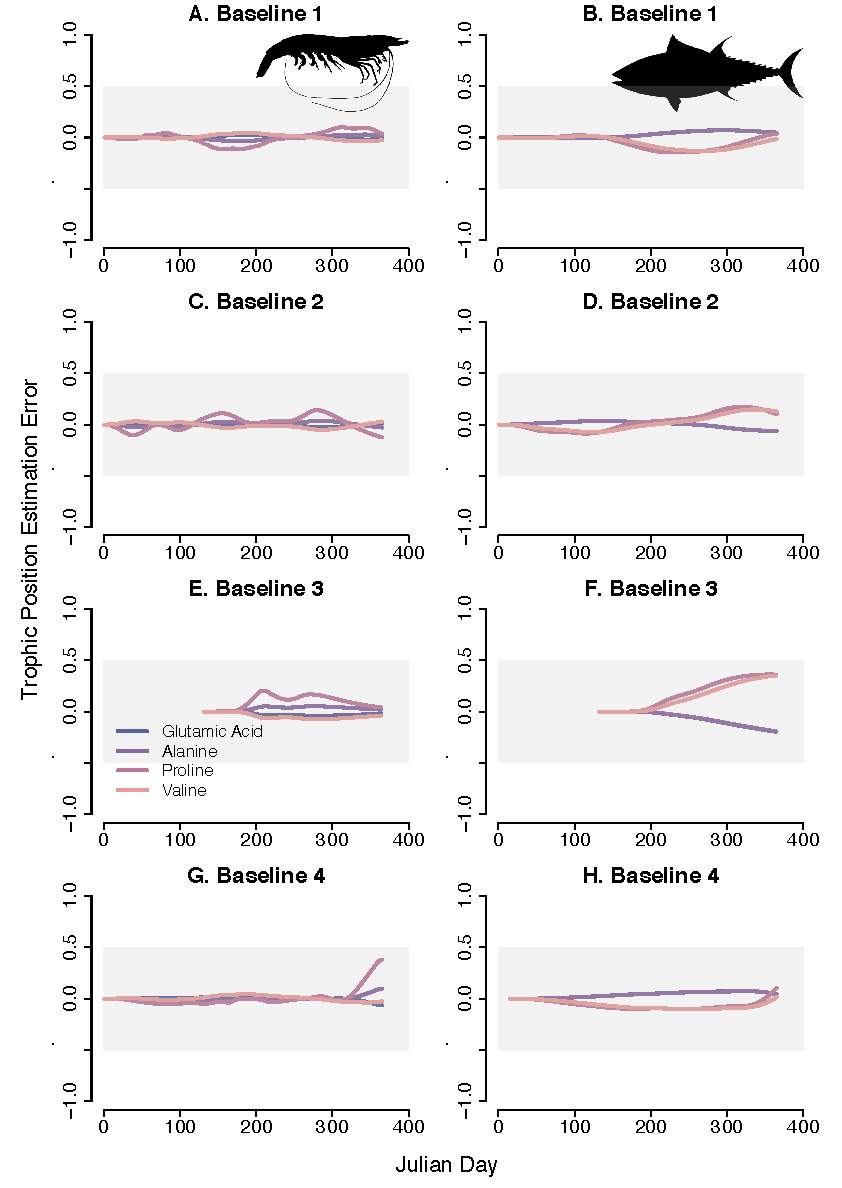
\includegraphics[width=0.55\textwidth]{figure/Ch5/Figure7.pdf}
  \caption{CSIA simulated trophic position}
  \label{fig:CSIATP}
\end{figure}
\clearpage

\textbf{Figure} \ref{fig:SensBSIA}: Sensitivity analysis of the
magnitude of trophic position estimation error from bulk stable isotope
values in response to primary, secondary, and tertiary (color) consumer
stable isotope half-life values for a single simulated stable isotope
baseline (a). Solid line denotes mean magnitude of estimation error
across the 125-day baseline simulation (A) for a given half-life and
shaded region denotes 1 standard deviation from the mean. 0, in B-D,
represents the true trophic level of a consumer. \newline 
\begin{figure}[h]
\centering
  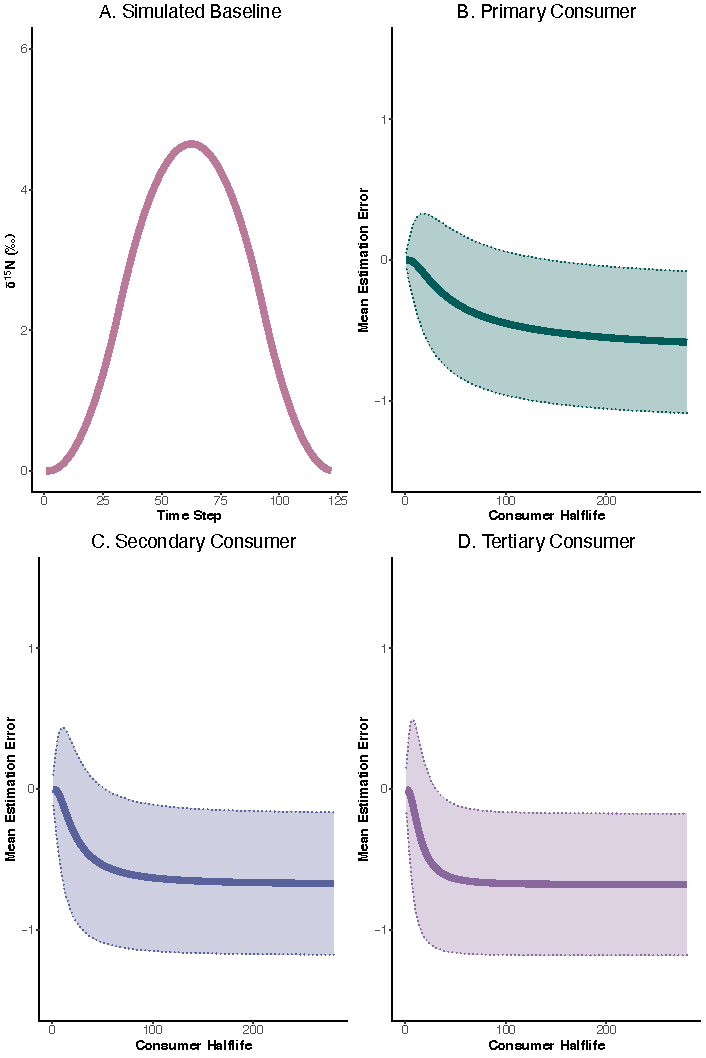
\includegraphics[width=0.55\textwidth]{figure/Ch5/Figure8.pdf}
  \caption{BSIA tissue turnover sensitivity analysis}
  \label{fig:SensBSIA}
\end{figure}
\clearpage

\textbf{Figure} \ref{fig:SensCSIAlys}: Sensitivity analysis of the
magnitude of trophic position estimation error from CSIA for primary,
secondary, and tertiary (color) consumer stable isotope half-life values
for a single simulated stable isotope baseline (a). The source amino
acid line denotes the single half-life value (130 days, lysine tuna) of
the source amino acid modelled in this analysis. Solid line denotes mean
magnitude of estimation error across the 125-day baseline simulation (A)
for a given half-life and shaded region denotes 1 standard deviation
from the mean. 0, in B-D, represents the true trophic level of a
consumer. \newline 
\begin{figure}[h]
\centering
  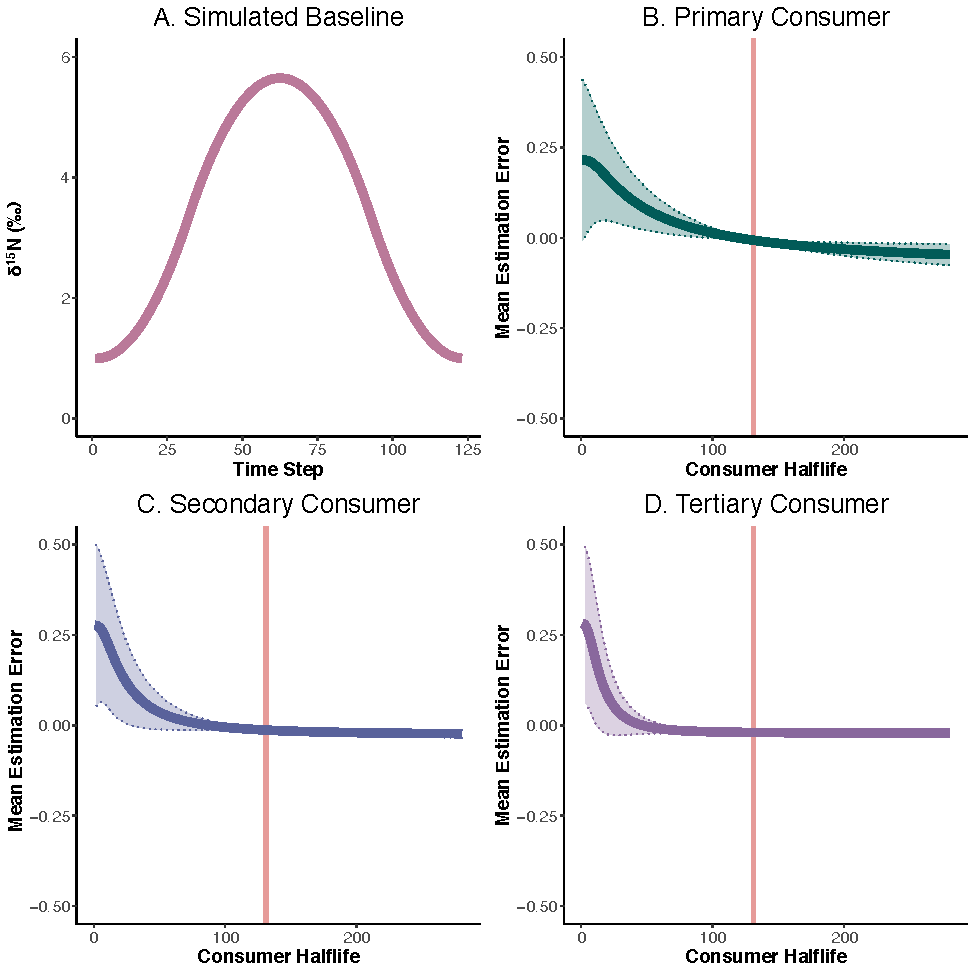
\includegraphics[width=0.75\textwidth]{figure/Ch5/Figure9.pdf}
  \caption{CSIA tissue turnover sensitivity analysis: lysine}
  \label{fig:SensCSIAlys}
\end{figure}
\clearpage

\textbf{Figure} \ref{fig:SensCSIAphe}: Sensitivity analysis of the
magnitude of trophic position estimation error from CSIA for primary,
secondary, and tertiary (color) consumer stable isotope half-life values
for a single simulated stable isotope baseline (a). The source amino
acid line denotes the single half-life value (33 days, phenylamine in
shrimp) of the source amino acid modelled in this analysis. Solid line
denotes mean magnitude of estimation error across the 125-day baseline
simulation (A) for a given half-life and shaded region denotes 1
standard deviation from the mean. 0, in B-D, represents the true trophic
level of a consumer. \newline
\begin{figure}[h]
\centering
  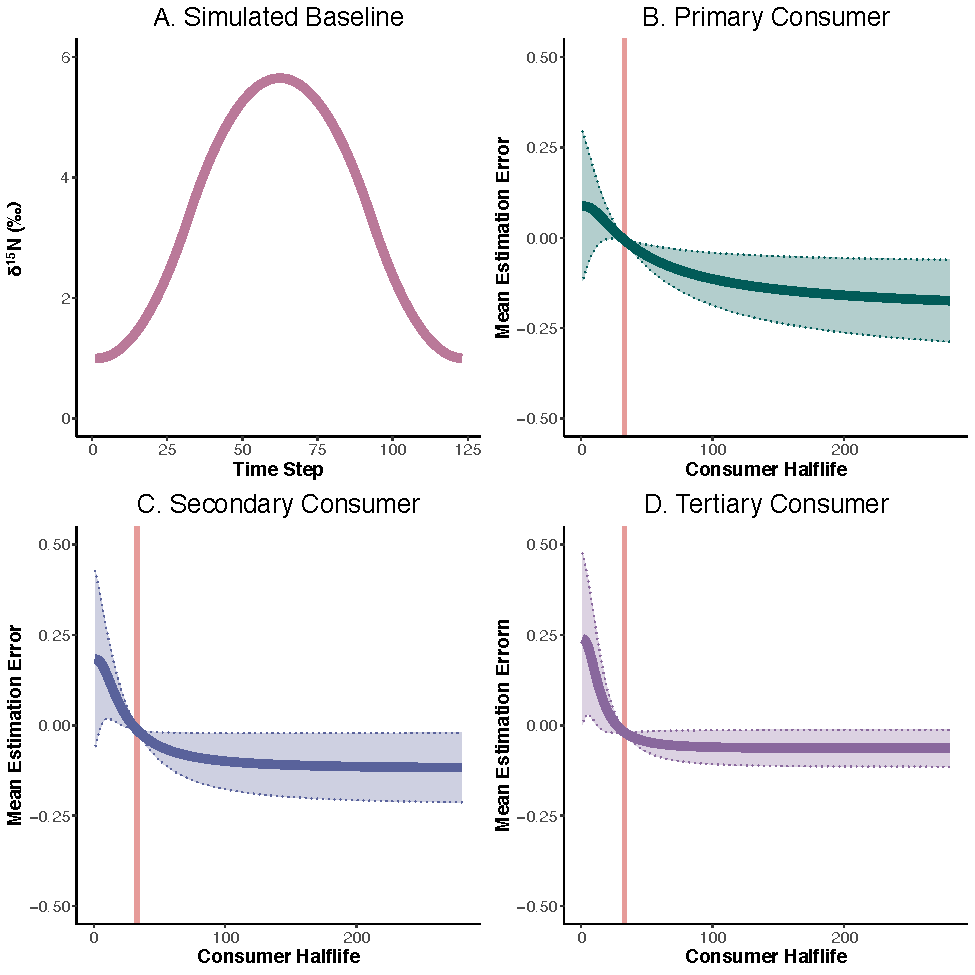
\includegraphics[width=0.75\textwidth]{figure/Ch5/Figure10.pdf}
  \caption{CSIA tissue turnover sensitivity analysis: phenylalanine}
  \label{fig:SensCSIAphe}
\end{figure}
\clearpage

\textbf{Figure} \ref{fig:TissueTurn}: Nitrogen stable isotope half-life
values (days) experimentally derived for a) bulk stable isotope analysis
(M. J. Vander Zanden et al.,
\protect\hyperlink{ref-VanderZanden2015}{2015}) for different species
(label) and tissues (color) and b) CSIA half-life values of individual
amino acids (Downs et al. and Popp et al.) for different species (color)
and amino acids (label). \newline
\begin{figure}[h]
\centering
  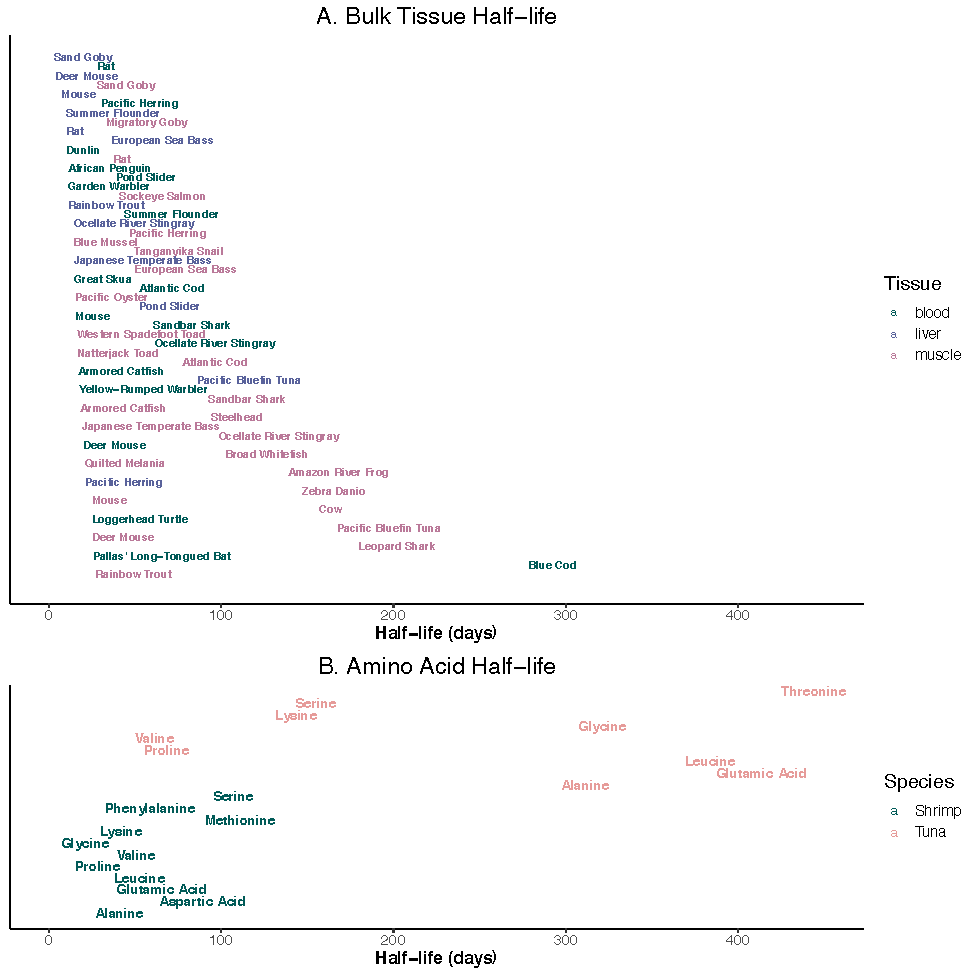
\includegraphics[width=0.85\textwidth]{figure/Ch5/Figure11.pdf}
  \caption{Observed tissue half-life values}
  \label{fig:TissueTurn}
\end{figure}
\clearpage

\textbf{Figure} \ref{fig:BSIATP2}: Trophic position estimation error
based on simulated primary, secondary, and tertiary consumer bulk
nitrogen stable isotope values (\(\delta^{15}N\)) for six (A-F) food web
scenarios (Figure 5.1) using the primary consumer stable isotope values
to calculate trophic position. 0 denotes the true trophic level of a
given consumer and grey box denotes trophic position deviation of ± 0.5
trophic levels used to calculate duration of deviation. \newline 
\begin{figure}[h]
\centering
  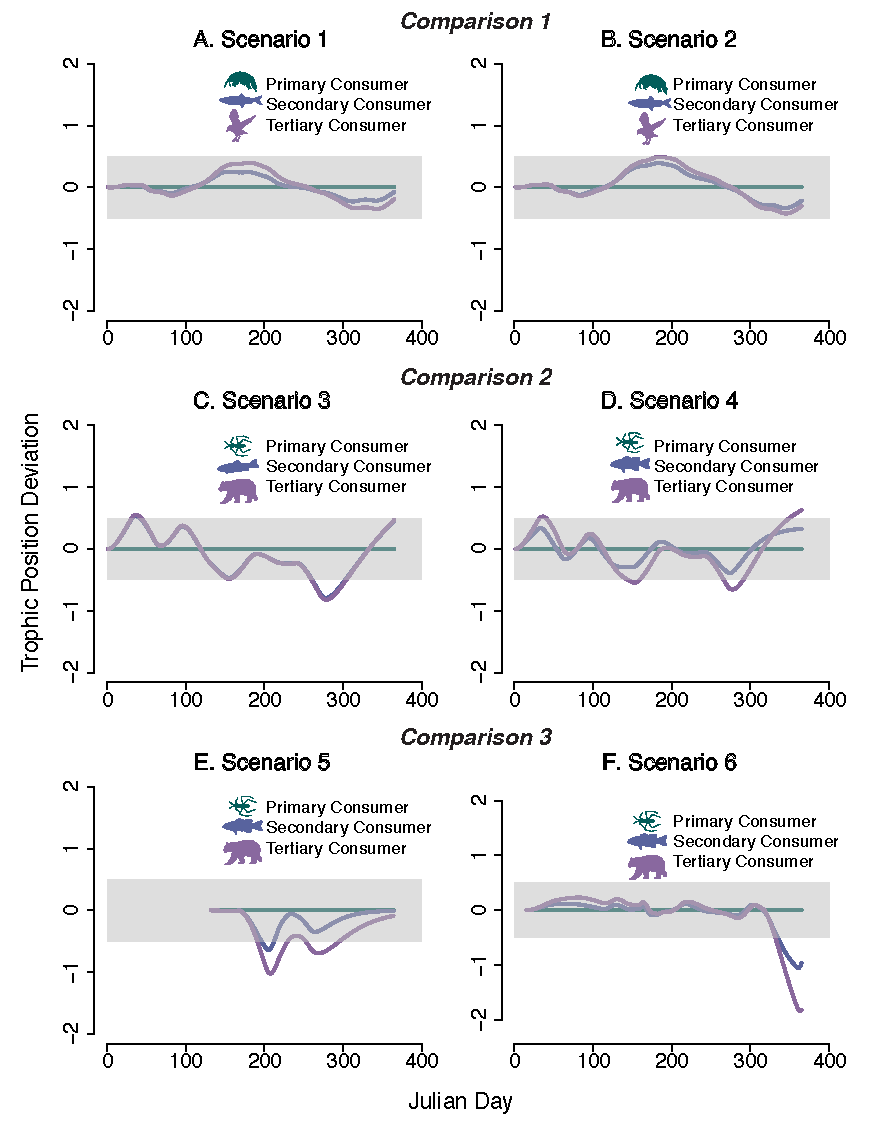
\includegraphics[width=0.6\textwidth]{figure/Ch5/Figure12.pdf}
  \caption{BSIA simulated trophic position: primary consumer baseline}
  \label{fig:BSIATP2}
\end{figure}
\clearpage

\chapter*{Conclusion}\label{conclusion}
\addcontentsline{toc}{chapter}{Conclusion}

This dissertation identified novel applications CSIA. In many studies,
the physiological challenges of measuring stable isotope data (i.e.,
tissue turnover time) are often framed as a hindrance for data
interpretation. In this dissertation I demonstrated that incorporating
the physiological and biogeochemical conditions that influence stable
isotope chemistry in consumers into study design can elucidate more
information for a system of interest. For example, applying temporal
lags based on tissue turnover times can identify delayed food web
responses to ecological change. This research provides a detailed
framework for incorporating stable isotope fractionation, tissue
turnover time, beta values, and resource use into the study design and
interpretation of CSIA data. Without consideration for each of these
components of stable isotope chemistry, there will be errors in trophic
position estimation and mixing model results that will hinder data
interpretation and potentially result in misleading conclusions.

Without accurate representation of the nitrogen fractionation that
occurs when organic nitrogen is transformed to inorganic sources
(mineralization, nitrification) contributions of salmon as a nutrient
source to vegetation will be overestimated and is likely overestimated
in previous marine derived nitrogen studies. The application of stable
isotope mixing models requires accurate stable isotope end members to
estimate dietary sources to consumers. When mixing models are applied to
vegetation, consideration for the direct sources of nitrogen that plants
``consume'' are necessary (i.e., ammonium, nitrate, amino acids). My
finding that soil ammonium is substantially enriched in \(^{15}N\)
compared to salmon tissue demonstrates salmon should not be used as an
end member in mixing models applied to plants because it does not
consider fractionation that occurs in soils. Understanding the
contributions of salmon to the riparian environment also requires
careful selection of a study site that has salmon present and a second
control site without salmon. Control sites usually consider the
composition of tree and vegetation community, but do not typically
consider soil composition. I observed substantial site variability with
distance from the same stream for sites previously used as controls.
Slope, aspect, gravimetric water content, and soil type are just a few
conditions that can alter nutrient content, fractionation in soil, and
tree growth, and if not accounted for can lead to misinterpretations of
marine derived nutrient studies. Conclusions from studies that do not
confirm soil conditions are comparable between `salmon' and `control'
sites should be interpreted with caution. Finally, marine derived
nutrient studies should focus on measuring ecological responses to
salmon presence rather than measuring the presence of marine derived
nutrients from stable isotopes and assuming the presence of enriched
nitrogen equates to increased nitrogen availability that will elicit an
ecological response. My results found differences in marine derived
nutrients with salmon presence but not increases in long-term nitrogen
availability or transformation rates. Studies should focus on the
ecological response (i.e., increased nitrogen transformation rates,
increased tree growth) between `salmon' and `control' sites and apply
stable isotopes to support the interpretation that ecological responses
are due to salmon contributions.

I demonstrated source amino acids provide novel information about how
nitrogen moves through and is utilized by food webs, particularly for
retrospective analyses. Studies focused on understanding nitrogen
resources directly measure phytoplankton blooms or nitrogen
concentrations and datasets are only available for small areas and short
periods of time. This presents a challenge of scale, both spatially and
temporally, when trying to understand how these measurements contribute
to mobile, large bodied, slow growing, marine consumers that integrate
resources from over broader spatial ranges and longer time scales. The
unique qualities of source amino acids that make them useful as an
indicator of stable isotope baseline for consumers, also means they can
serve as an important tracer on their own. Notably, source amino acids
are still susceptible to the challenges in interpreting stable isotope
values of nitrogen that occur from fractionation from nitrogen
transformations, phytoplankton assimilation, and trophic enrichment.
Therefore, the most interpretable and useful applications of source
amino acid studies will trace long-term contributions of nitrogen
sources with distinct stable isotope values. Sea ice derived algae is
one example of a nitrogen sources that is enriched in 15N and measurable
in consumer tissues based on our results. Measuring the nitrogen stable
isotope values of source amino acids from historic and contemporary
samples from environments where sea ice derived algae has been known to
change due sea ice decline and oceanic warming such as Baffin Bay, could
inform how food webs adapt their resource use in a changing world.

Measuring trophic position in consumers such as harbor seals is useful
for understanding general ecosystem change but identifying the specific
mechanism that caused the trophic position change requires additional
information. Some climate drivers were strong predictors of both source
amino acid stable isotope values and trophic position estimates, but
others were only good predictors of trophic position estimates. This is
particularly relevant when trying to identify mechanisms of climate
forcing on the food web. One approach for identifying whether the
mechanisms of climate forcing is constraining nutrients at the base of
the food web or is acting on recruitment and growth higher in the food
web, is to combine analyses of both trophic position and source amino
acids. For example, freshwater discharge impacts harbor seal trophic
position and source amino acid stable isotope values. Therefore, climate
variables are directly influencing nitrogen at the base of the food web
which then is propagating through the food web and altering harbor seal
trophic level. In contrast, sea surface temperature only impacted harbor
seal trophic position, meaning it was altering abundance of mid trophic
level species (likely forage fish) and that was the mechanism that was
ultimately causing a trophic shift. Applying CSIA to mid trophic level
species in addition to a top predator would provide a more complete
picture of causal mechanisms of trophic level change of top predators.
Specifically, it could identify if the trophic level change was
occurring in the top predator (if the lower trophic level species did
not also have a shift) or if it was occurring lower in the food web (if
both species experienced a trophic level change).

Trophic position change can be difficult to interpret, particularly for
high trophic level, generalist predators like harbor seals. Trophic
position can change due to a dietary shift by the consumer of interest,
a shift lower in the food web, or a shift in protein quality of prey.
These mechanisms are more easily resolved when applying CSIA to
specialist species compared to a generalist. One potential application
would be the southern resident killer whale (SRKW) in Washington, that
consumes exclusively salmon. Applying CSIA to SRKW would eliminate the
potential of protein quality influencing data interpretation (due to the
exclusively piscivorous diet) therefore a trophic level change in SRKW
would indicate consumption of smaller salmon. This could be the result
of eating a greater number of smaller species such as pink salmon, or
smaller individuals of Chinook salmon. While the exact mechanism would
still not be identified from CSIA data alone, it would identify a change
in the SRKW -- salmon relationship and if combined with pacific Salmon
abundance and size data which are collected annually, it would offer a
more complete picture of the dynamics of this relationship through time
than abundance data alone.

Ecological integrity indicators have been incorporated into the
California Current Integrated Ecosystem Assessment and include
indicators of trophic structure such as mean groundfish trophic level.
Harbor seal trophic position could be a useful addition to these
datasets. This dissertation provides a historic baseline which
contemporary data can be compared to. In addition, contemporary mean
groundfish trophic level is collected annually. Combined, these two
datasets are a powerful tool for measuring ecological integrity. The
addition of harbor seal data would determine whether changes in
ecological integrity span the entire food web and identify whether
observed changes are confined to certain parts of the food web. For
example, if changes were observed in harbor seals but not groundfish
that would indicate predators were modifying their foraging strategies.
If a change was observed in both groundfish and harbor seals, then it
would indicate a bottom-up effect propagating through the entire food
web. Collection of harbor seal trophic position data for indicators
would ideally occur annually, but data that is pooled over 1-5 years
should be sufficient for identifying widescale ecological change, as
this dissertation shows harbor seal trophic position response to food
web and climate conditions are often delayed by multiple years. A
continuous sampling strategy may be able to be incorporated into marine
mammal stranding networks. Pooling data on decadal scales may be more
feasible, but it comes with the risk of overlooking potential food web
responses based on how the decadal breakpoints correspond temporally
relative to the ecological change. Alternatively, samples could be
collected in the two years following major climate perturbations. Given
the lagged response due to both tissue turnover and propagation of
ecological conditions up the food web, and the increase in extreme
climate events over the past two decades, it would be possible to
retroactively analyze the effects of extreme climate conditions on the
food web by measuring predator tissues in the 1-3 years following the
event.

Compound-specific stable isotope analysis can provide novel information
regarding ecological and biogeochemical responses to climate change. An
important component to the application and interpretation of this type
of data is the physiological and biogeochemical parameters that
influence stable isotope fractionation. With my dissertation as a
foundation future work can better constrain assumptions of stable
isotope parameters to reconstruct historic datasets and apply CSIA data
to understand delayed food web responses and resource assimilation into
food webs.

\appendix

\chapter{Appendix 1}\label{appendix-1}

\section{Text 1: Full analytical details for stable
isotopes}\label{text-1-full-analytical-details-for-stable-isotopes}

Collagen samples have been analyzed for both CSSIA and bulk
\(\delta^{15}N\) which require 10 mg of purified collagen (100 mg of
bone). Preliminary analyses were conducted to determine the highest rate
of collagen return from bone sampled from different parts of the skull
to minimize destruction. Samples were taken from the internal occipital
shelf to maintain external integrity. Bone was decalcified using 0.2 M
HCl for 24-72 hours depending on bone thickness, followed by
centrifugation and nanopure water rinse. Removal of humic acids was
conducted using 0.125 M NaOH for 20 hours. Samples were washed to a
neutral pH, then solubilized in 0.01N HCl. Once solubilized samples were
blown down under N2 to prevent isotopic fractionation, and freeze dried.
Freeze dried collagen was be analyzed for bulk isotopic composition of
nitrogen by the UW IsoLab (isolab.ess.washington.edu) using a coupled
elemental analyzer-isotope ratio mass spectrometer following the
standard protocols of the laboratory. C:N ratios were calculated from
this data, which is a measure of the quality for carbon and nitrogen
analyses of bone collagen for isotopic analysis. Only three observations
were outside of the acceptable rang of 2.7-3.6; indicating there was no
substantial loss of glycine or addition of nitrogen due to microbial
processing from mortality, decay, curation, and analysis.

\(\delta^{15}N\) of eleven amino acids were measured in the UW Facility
for Compound-Specific Isotope Analysis of Environmental Samples. Samples
were prepared following the procedures developed by Popp Marine Lab at
University of Hawaii Manoa. Briefly, proteins were hydrolyzed in 6N HCl
and purified using a cation exchange column. Amino acids were esterified
using isopropanol acetyl chloride, and derivatized via acylation with
4:1 toluene: pivaloyl chloride. Samples were brought up in ethyl acetate
and analyzed using a coupled gas chromatography-combustion-isotope ratio
mass spectrometer system (GC-C-irMA; Thermo Scientific Trace GC + GC
IsoLink coupled to a Delta V irMS) in continuous flow mode monitoring
masses (m/z) 28 and 29 using a db-35 column. For each run a 12 amino
acid external standard with known isotopic composition was injected
three times followed by sample injections. Samples were injected in
triplicate, with the 12 amino acid standard injected every two samples
(or six injections). A two-hour column oxidation was performed after 6
samples (25 injections). Samples and standards included norleucine as an
internal standard.

For each machine run, a linear model was fit for each individual amino
acid using the following equation:
\begin{equation} 
  Std_{aa} = m_{aa}t + b_{aa}
  \label{eq:std}
\end{equation}
Where m represents the slope of the precision drift, \emph{t} represents
the injection number since last column oxidation, and \emph{Std}
represents the \(\delta^{15}N\) of an individual amino acid for a
standard observation. The data was then corrected using the following
equations:
\begin{equation} 
  D_{aa, t} = Std_{aa,t} - True
  \label{eq:diff}
\end{equation}
Where \(D_{aa,t}\) is the difference between an observed standard
\(\delta^{15}N\) of \(Std_{aa,t}\) for a given amino acid at a given
injection number and the true \(\delta^{15}N\) for that standard. Then:
\begin{equation} 
  Sample_{corrected,aa,t} = Sample_{obs,aa,t} - D_{aa,t}
  \label{eq:sampcorr}
\end{equation}
Where the drift value, \(D_{aa,t}\), is subtracted from the sample value
for a given amino acid and a given injection to correct the observed
sample values for precision drift since last column oxidation. Mean
sample corrected values for the triplicate injections were used for all
amino acid \(\delta^{15}N\).

\section{Text 2: Identifying size and sex-based trends in harbor seal
trophic
position}\label{text-2-identifying-size-and-sex-based-trends-in-harbor-seal-trophic-position}

Only a subset of the samples included month of collection, sex, and
length metadata and therefore separate month, length, and sex specific
analyses were fit to the data to test whether they should be considered
as predictors for the ocean condition and prey availability data.
Standard linear models with: 1) sex as a factor, 2) length as a
continuous covariate and 3) month as a continuous covariate were fit to
both Salish Sea and coastal WA for each individual trophic amino acid.
These models were used to test whether trophic position varies with
length and sex, whether these trends are consistent between amino acids,
and whether one year was an appropriate approximation for tissue
turnover of bone collagen. The standard linear models took the following
structure:
\begin{equation} 
 y_i \sim N(\boldsymbol{\alpha}_{j[i]} + \boldsymbol{\beta}_{j[i]}\boldsymbol{x}_i, \sigma^2_y)
  \label{eq:hiermods2}
\end{equation}
where \emph{y} represents harbor seal trophic position calculated from
phenylalanine and a trophic amino acid \emph{i}, \(\boldsymbol{X}\) is a
matrix of bottom-up drivers for a given model, \(\boldsymbol{\beta}\) is
a vector of covariates (sex, length, month, location), and \emph{a} is
the intercept. There were no significant differences in trophic position
between male and female harbor seals in either the Salish Sea (Figure
\ref{fig:sexWA}A) or coastal Washington (Figure \ref{fig:sexWA}B); this
relationship was consistent across amino acids. Similarly, trophic
position did not change based on harbor seal length (Figure
\ref{fig:lengthWA}). Interestingly, the exception to this finding was
trophic position calculated by proline, which showed a significant
decline with size. Mean harbor seal trophic position calculated from
proline for harbor seals ranging from 150 - 180 cm in standard was 0.6
lower than harbors seals that were less than 120 cm of standard length
(Figure \ref{fig:lengthWA}). Trophic position calculated from alanine,
aspartic acid and valine also showed negative trends with size, although
the trend was not statistically significant, while trophic position
calculated from glutamic acid was positive but also not statistically
significant. There was also no observed `seasonality' in harbor seal
trophic position (Figure \ref{fig:season}) indicating 1-year
physiological delay was a reasonable approximation for tissue turnover
time of skull bone collagen.

Harbor seals in Washington do not have distinct trophic ecology based on
adult size (Figure \ref{fig:sexWA}) or sex (Figure \ref{fig:lengthWA}).
Bjorkland et al. (\protect\hyperlink{ref-Bjorkland2015}{2015}) did not
observe sex or size (weight) based differences in bulk \(\delta^{15}N\)
values in harbor seals in the San Juan Islands in the Salish Sea between
2007 and 2008. Our results agree with this finding and with similar
studies of other Pacific pinniped species (Dehn et al.,
\protect\hyperlink{ref-Dehn2007}{2007}; Drago, Cardona, Crespo, \&
Aguilar, \protect\hyperlink{ref-Drago2009}{2009}). While both male and
female harbor seals have a similar trophic position, it is possible sex
and size-based differences in foraging strategies within a similar
trophic position exist (Bjorkland et al.,
\protect\hyperlink{ref-Bjorkland2015}{2015}; K. Wilson et al.,
\protect\hyperlink{ref-Wilson2014}{2014}). Additionally, this study
focused on adult harbor seals and changes in trophic position between
juveniles, sub adults and adults are possible as indicated by pinniped
studies (Zhao, Castellini, Mau, \& Trumble,
\protect\hyperlink{ref-Zhao2004}{2004}). Regardless, our results show
long-term consistencies in the trophic niche exploited by both male and
female harbor seals regardless of adult size in Washington.

\section{Text 3: Identifying temporal trends in harbor seal trophic
position}\label{text-3-identifying-temporal-trends-in-harbor-seal-trophic-position}

To understand any changes through time to harbor seal foraging ecology
over the past 100 years that were not explained by the tested
environmental and food web covariates (Tables \ref{tab:ocmod} \&
\ref{tab:prmod}), generalized additive models (GAMs) were fit the
residuals for the best ocean condition-prey model with a smooth term by
year and a k term of 5. These analyses (Figures 3.6 \& 3.7) were
compared to the raw time series of harbor seal trophic position data
(Figure \ref{fig:year}) to identify trends through time that are
unexplained by the covariates included in this analysis.

Trends in harbor seal trophic position through time were different
between the Salish Sea and coastal Washington (Figure \ref{fig:year}).
The time series of the glutamic acid trophic position in coastal
Washington had a significant positive trend through time (Figure
\ref{fig:year}b) that increased from 1948-1968 and remained relatively
constant following 1975. Trophic position calculated from alanine and
proline showed similar trends, although the alanine trophic position
trend was not statistically significant (Figure \ref{fig:year}a). In
contrast, harbor seal trophic position in the Salish Sea calculated from
glutamic acid, alanine, aspartic acid, and proline has been relatively
stable over the past century, but the trophic position calculated from
valine showed a significant decline since 1968.

There were no trends through time for the model residuals for any amino
acid after accounting for environmental (Figure 3.6) and food web
(Figure 3.7) conditions at all three time lags. This indicates that prey
availability and ocean conditions account for most temporal variation
observed in the trophic position time series (Figure \ref{fig:year}).
However, valine was a notable exception, which demonstrated a decreasing
trend through time in model residuals for all of the models with the
most support.

\section{Text 4: Accounting for variability in trophic enrichment
factors}\label{text-4-accounting-for-variability-in-trophic-enrichment-factors}

Trophic enrichment factors are variable based on animal diet (omnivory,
carnivory, herbivory), pathways of nitrogen excretion, and trophic level
(McMahon et al., \protect\hyperlink{ref-McMahon2015}{2015}; J. M.
Nielsen et al., \protect\hyperlink{ref-Nielsen2015}{2015}) with
ominvory, carnivory and higher trophic levels demonstrating the lowest
trophic enrichment for most amino acids. Trophic enrichment has
ultimately been attributed to diet quality (similarity in tissues
between consumer and prey) and mode of nitrogen excretions, although the
relative impacts of each is difficult to discern, especially considering
most controlled feeding studies include low-trophic level ammonia
excretion but not high trophic level species (i.e., adult hake or
salmon). In coastal Washington, most trophic transfers are between high
diet quality, piscivorous fish (ammonia excretion) with a high-quality
transfer between fish and harbor seal (urea excretion). Studies using
multiple trophic enrichment factors based on the food web structure and
consumption type produce more accurate trophic position estimations
especially for higher level consumers (Kelton \& Matthew,
\protect\hyperlink{ref-McMahon2016}{2016}; McMahon et al.,
\protect\hyperlink{ref-McMahon2019}{2019},
\protect\hyperlink{ref-McMahon2015}{2015}).

We applied multiple trophic position calculation frameworks for harbor
seals to determine the best approach (Table \ref{tab:tpparam}) by
identifying the percentage of data that fell within an ecologically
realistic trophic position range for harbor seals. We also applied these
approaches to herring, a known harbor seal prey species, with data from
Germain et al. (\protect\hyperlink{ref-Germain2013}{2013}). Based on
known foraging patterns, we anticipate harbor seals have an average
trophic position of 3.5 to 5 and herring will have an average trophic
position of 2.5-2.9. Equation 2 from (Figure \ref{fig:nvbeta}.2)
produced the most accurate herring trophic position estimates for most
amino acids, however valine produced an impossibly low estimate of
trophic position. In contrast, equation 3 (Figure \ref{fig:nvbeta}.3)
produced the most accurate results for most amino acids compared to
harbor seals, but these estimates were still unrealistically low for
some amino acids (proline, valine), which is common for CSIA (Kelton \&
Matthew, \protect\hyperlink{ref-McMahon2016}{2016}). Additionally, this
is not the most ecologically accurate parameterization, as it assumes
all trophic transfers are of high prey quality, where there must be at
least one herbivorous-low quality trophic transfer in the food web from
phytoplankton to zooplankton (parameterization of equation 4, Figure
\ref{fig:nvbeta}.4). It also assumes prey quality (carnivorous) and
trophic level of the consumer is more important than nitrogen excretion
pathway (urea versus ammonia) for some amino acids but not others.
Seemingly, these assumptions impact trophic position estimates from
individual trophic amino acids differently which will likely be an
important consideration for future studies applying a multi-amino acid
framework. It is possible that these reflect biases in conventional
trophic position estimates (i.e., stomach content analysis) as proposed
by McMahon et al. (\protect\hyperlink{ref-McMahon2015}{2015}) or there
may be biases in controlled feeding studies. For example, growth rate of
individuals in controlled feeding studies may not accurately reflect
those in natural ecosystems which may lead to overestimates in trophic
enrichment if they are higher in natural systems compared to controlled
feeding experiments. This may be plausible in the Washington food web as
consumption of juvenile fish is common at multiple trophic levels, and
juveniles presumably have higher growth rates than adults.

Mean harbor seal trophic position estimates were similar across trophic
amino acids however some were more variable than others. The standard
deviation of trophic position was higher for proline (4.6 ± 0.7, mean ±
1SD), and valine (3.7 ± 0.8) and included more ecologically unrealistic
values compared to glutamic acid (4.5 ± 0.4) and alanine (3.9 ± 0.4).
Trophic position calculated from aspartic acid (4.1 ± 1.0) had the
highest standard deviation and also demonstrated a trend through time
compared to other amino acid trophic position calculations (Figure
\ref{fig:year}).

Application of a multi-amino acid trophic position calculation 1)
offered a more realistic parameterization of the trophic position
equation, 2) improved model certainty and 3) produced similar covariate
coefficients compared to a glutamic acid only parameterization.
Examination of the distribution of trophic position calculations for
each individual trophic amino acid shows variability in accuracy and
variance for single trophic amino acid calculations (Figures
\ref{fig:nbeta} \& \ref{fig:nvbeta}). For example, aspartic acid had a
much wider variance compared to other amino acids (Figures
\ref{fig:nbeta} \& \ref{fig:nvbeta}) and also produced different trends
through time (Figure \ref{fig:year}).

It is likely differences in tissue turnover time between individual
amino acids and phenylalanine contribute to the variance of the trophic
position estimates derived from individual trophic amino acids. Downs et
al. (\protect\hyperlink{ref-Downs2014}{2014}) found phenylalanine takes
780 hours to reach 50\% turnover in shrimp. This is comparable to
glutamic acid, alanine, and valine which take 940, 642, and 942 hours
respectively which are substantially lower than aspartic acid which
requires 1530 hours. The discrepancy between tissue turnover times
between aspartic acid and phenylalanine is likely the cause of the broad
distribution for aspartic acid derived trophic position compared to
other trophic amino acids, as aspartic acid is incorporating the
nitrogen isotope signature over a substantially larger time period
relative to phenylalanine and thus may incorporate more prey switching
and/or changes in the isotopic signature of primary producers.

Addition of alanine to the glutamic acid only model resulted in the
largest difference in model certainty. A glutamic acid -- alanine model
supported the same best models for both the environmental and prey
models at all time lags. The combined tissue turnover of glutamic acid
and alanine of shrimp (791 hours) is very similar to that of
phenylalanine (780 hours) ensuring both the trophic and source amino
acids were incorporated over a similar time scale (albeit the trophic
amino acids were a wider time scale). Benefits of a multi-amino acid
trophic position equation may not require four amino acids as previously
suggested (J. M. Nielsen et al.,
\protect\hyperlink{ref-Nielsen2015}{2015}) but rather carefully selected
trophic amino acids to ensure the trophic amino acids are incorporated
over a similar time scale as the source amino acids. If tissue turnover
times are unable to be approximated, utilizing four trophic amino acids
or two source amino acids as suggested by J. M. Nielsen et al.
(\protect\hyperlink{ref-Nielsen2015}{2015}) would likely provide the
same benefit as fewer, carefully selected amino acids based on tissue
turnover times.

\chapter*{Colophon}\label{colophon}
\addcontentsline{toc}{chapter}{Colophon}

This document is set in \href{https://github.com/georgd/EB-Garamond}{EB
Garamond}, \href{https://github.com/adobe-fonts/source-code-pro/}{Source
Code Pro} and \href{http://www.latofonts.com/lato-free-fonts/}{Lato}.
The body text is set at 11pt with \(\familydefault\).

It was written in R Markdown and \(\LaTeX\), and rendered into PDF using
\href{https://github.com/benmarwick/huskydown}{huskydown} and
\href{https://github.com/rstudio/bookdown}{bookdown}.

This document was typeset using the XeTeX typesetting system, and the
\href{http://staff.washington.edu/fox/tex/}{University of Washington
Thesis class} class created by Jim Fox. Under the hood, the
\href{https://github.com/UWIT-IAM/UWThesis}{University of Washington
Thesis LaTeX template} is used to ensure that documents conform
precisely to submission standards. Other elements of the document
formatting source code have been taken from the
\href{https://github.com/stevenpollack/ucbthesis}{Latex, Knitr, and
RMarkdown templates for UC Berkeley's graduate thesis}, and
\href{https://github.com/suchow/Dissertate}{Dissertate: a LaTeX
dissertation template to support the production and typesetting of a PhD
dissertation at Harvard, Princeton, and NYU}

The source files for this thesis, along with all the data files, have
been organised into an R project, Dissertation, which is available at
\url{https://github.com/mfeddern/Dissertation}. A hard copy of the
dissertation can be found in the University of Washington library.

This version of the thesis was generated on 2021-12-01 13:17:20. The
repository is currently at this commit:

The computational environment that was used to generate this version is
as follows:
\begin{verbatim}
- Session info ---------------------------------------------------------------
 setting  value                       
 version  R version 4.0.2 (2020-06-22)
 os       macOS Catalina 10.15.6      
 system   x86_64, darwin17.0          
 ui       X11                         
 language (EN)                        
 collate  en_US.UTF-8                 
 ctype    en_US.UTF-8                 
 tz       America/Los_Angeles         
 date     2021-12-01                  

- Packages -------------------------------------------------------------------
 package     * version date       lib source                               
 assertthat    0.2.1   2019-03-21 [1] CRAN (R 4.0.0)                       
 backports     1.1.6   2020-04-05 [1] CRAN (R 4.0.0)                       
 bookdown      0.22.3  2021-05-22 [1] Github (rstudio/bookdown@aa75b5f)    
 callr         3.7.0   2021-04-20 [1] CRAN (R 4.0.2)                       
 cli           2.5.0   2021-04-26 [1] CRAN (R 4.0.2)                       
 colorspace    1.4-1   2019-03-18 [1] CRAN (R 4.0.0)                       
 crayon        1.3.4   2017-09-16 [1] CRAN (R 4.0.0)                       
 desc          1.2.0   2018-05-01 [1] CRAN (R 4.0.0)                       
 devtools    * 2.3.1   2020-07-21 [1] CRAN (R 4.0.2)                       
 digest        0.6.27  2020-10-24 [1] CRAN (R 4.0.2)                       
 dplyr         1.0.2   2020-08-18 [1] CRAN (R 4.0.2)                       
 ellipsis      0.3.0   2019-09-20 [1] CRAN (R 4.0.0)                       
 evaluate      0.14    2019-05-28 [1] CRAN (R 4.0.0)                       
 fs            1.5.0   2020-07-31 [1] CRAN (R 4.0.2)                       
 generics      0.0.2   2018-11-29 [1] CRAN (R 4.0.0)                       
 ggplot2       3.3.0   2020-03-05 [1] CRAN (R 4.0.0)                       
 git2r         0.27.1  2020-05-03 [1] CRAN (R 4.0.2)                       
 glue          1.4.2   2020-08-27 [1] CRAN (R 4.0.2)                       
 gtable        0.3.0   2019-03-25 [1] CRAN (R 4.0.0)                       
 htmltools     0.5.1.1 2021-01-22 [1] CRAN (R 4.0.2)                       
 httr          1.4.2   2020-07-20 [1] CRAN (R 4.0.2)                       
 huskydown   * 0.0.5   2021-05-16 [1] Github (benmarwick/huskydown@addb48e)
 kableExtra    1.3.4   2021-02-20 [1] CRAN (R 4.0.2)                       
 knitr         1.33    2021-04-24 [1] CRAN (R 4.0.2)                       
 lifecycle     0.2.0   2020-03-06 [1] CRAN (R 4.0.0)                       
 magrittr      2.0.1   2020-11-17 [1] CRAN (R 4.0.2)                       
 memoise       1.1.0   2017-04-21 [1] CRAN (R 4.0.2)                       
 munsell       0.5.0   2018-06-12 [1] CRAN (R 4.0.0)                       
 pillar        1.4.3   2019-12-20 [1] CRAN (R 4.0.0)                       
 pkgbuild      1.0.6   2019-10-09 [1] CRAN (R 4.0.0)                       
 pkgconfig     2.0.3   2019-09-22 [1] CRAN (R 4.0.0)                       
 pkgload       1.0.2   2018-10-29 [1] CRAN (R 4.0.0)                       
 prettyunits   1.1.1   2020-01-24 [1] CRAN (R 4.0.0)                       
 processx      3.5.2   2021-04-30 [1] CRAN (R 4.0.2)                       
 ps            1.6.0   2021-02-28 [1] CRAN (R 4.0.2)                       
 purrr         0.3.4   2020-04-17 [1] CRAN (R 4.0.0)                       
 R6            2.4.1   2019-11-12 [1] CRAN (R 4.0.0)                       
 remotes       2.2.0   2020-07-21 [1] CRAN (R 4.0.2)                       
 rlang         0.4.11  2021-04-30 [1] CRAN (R 4.0.2)                       
 rmarkdown     2.8     2021-05-07 [1] CRAN (R 4.0.2)                       
 rprojroot     1.3-2   2018-01-03 [1] CRAN (R 4.0.0)                       
 rstudioapi    0.11    2020-02-07 [1] CRAN (R 4.0.0)                       
 rvest         0.3.6   2020-07-25 [1] CRAN (R 4.0.2)                       
 scales        1.1.0   2019-11-18 [1] CRAN (R 4.0.0)                       
 sessioninfo   1.1.1   2018-11-05 [1] CRAN (R 4.0.2)                       
 stringi       1.6.2   2021-05-17 [1] CRAN (R 4.0.2)                       
 stringr       1.4.0   2019-02-10 [1] CRAN (R 4.0.0)                       
 svglite       2.0.0   2021-02-20 [1] CRAN (R 4.0.2)                       
 systemfonts   1.0.2   2021-05-11 [1] CRAN (R 4.0.2)                       
 testthat      3.0.2   2021-02-14 [1] CRAN (R 4.0.2)                       
 tibble        3.0.1   2020-04-20 [1] CRAN (R 4.0.0)                       
 tidyselect    1.1.0   2020-05-11 [1] CRAN (R 4.0.0)                       
 usethis     * 1.6.1   2020-04-29 [1] CRAN (R 4.0.2)                       
 vctrs         0.3.4   2020-08-29 [1] CRAN (R 4.0.2)                       
 viridisLite   0.3.0   2018-02-01 [1] CRAN (R 4.0.0)                       
 webshot       0.5.2   2019-11-22 [1] CRAN (R 4.0.0)                       
 withr         2.4.2   2021-04-18 [1] CRAN (R 4.0.2)                       
 xfun          0.23    2021-05-15 [1] CRAN (R 4.0.2)                       
 xml2          1.3.2   2020-04-23 [1] CRAN (R 4.0.2)                       
 yaml          2.2.1   2020-02-01 [1] CRAN (R 4.0.0)                       

[1] /Library/Frameworks/R.framework/Versions/4.0/Resources/library
\end{verbatim}
\backmatter

\chapter*{References}\label{references}
\addcontentsline{toc}{chapter}{References}

\markboth{References}{References}

\noindent

\setlength{\parindent}{-0.20in} \setlength{\leftskip}{0.20in}
\setlength{\parskip}{8pt}

\hypertarget{refs}{}
\hypertarget{ref-Anderson2007}{}
Anderson, C., \& Cabana, G. (2007). Estimating the trophic position of
aquatic consumers in river food webs using stable nitrogen isotopes.
\emph{Journal of the North American Benthological Society},
\emph{26}(2), 273--285. Journal Article.
\href{http://doi.org/10.1899/0887-3593(2007)26\%5B273:ETTPOA\%5D2.0.CO;2}{http://doi.org/10.1899/0887-3593(2007)26{[}273:ETTPOA{]}2.0.CO;2}

\hypertarget{ref-Atkinson1996}{}
Atkinson, A. (1996). Subantarctic copepods in an oceanic, low
chlorophyll environment: Ciliate predation, food selectivity and impact
on prey populations. \emph{Marine Ecology. Progress Series
(Halstenbek)}, \emph{130}(1/3), 85--96. Journal Article.
\url{http://doi.org/10.3354/meps130085}

\hypertarget{ref-Atkinson2008}{}
Atkinson, S., Demaster, D. P., \& Calkins, D. G. (2008). Anthropogenic
causes of the western steller sea lion eumetopias jubatus population
decline and their threat to recovery. \emph{Mammal Review},
\emph{38}(1), 1--18. Journal Article.
\url{http://doi.org/10.1111/j.1365-2907.2008.00128.x}

\hypertarget{ref-Barbeaux2020}{}
Barbeaux, S. J., Holsman, K., \& Zador, S. (2020). Marine heatwave
stress test of ecosystem-based fisheries management in the gulf of
alaska pacific cod fishery. \emph{Frontiers in Marine Science},
\emph{7}. Journal Article. \url{http://doi.org/10.3389/fmars.2020.00703}

\hypertarget{ref-Barth2007}{}
Barth, J. A., Menge, B. A., Lubchenco, J., Chan, F., Bane, J. M.,
Kirincich, A. R., \ldots{} Washburn, L. (2007). Delayed upwelling alters
nearshore coastal ocean ecosystems in the northern california current.
\emph{Proceedings of the National Academy of Sciences - PNAS},
\emph{104}(10), 3719--3724. Journal Article.
\url{http://doi.org/10.1073/pnas.0700462104}

\hypertarget{ref-Bartz2005}{}
Bartz, K. K., \& Naiman, R. J. (2005). Effects of salmon-borne nutrients
on riparian soils and vegetation in southwest alaska. \emph{Ecosystems
(New York)}, \emph{8}(5), 529--545. Journal Article.
\url{http://doi.org/10.1007/s10021-005-0064-z}

\hypertarget{ref-Benbow2020}{}
Benbow, M. E., Receveur, J. P., \& Lamberti, G. A. (2020). Death and
decomposition in aquatic ecosystems. \emph{Frontiers in Ecology and
Evolution}, \emph{8}. Journal Article.
\url{http://doi.org/10.3389/fevo.2020.00017}

\hypertarget{ref-Bi2020}{}
Bi, R., \& Sommer, U. (2020). Food quantity and quality interactions at
phytoplankton--Zooplankton interface: Chemical and reproductive
responses in a calanoid copepod. \emph{Frontiers in Marine Science},
\emph{7}. Journal Article. \url{http://doi.org/10.3389/fmars.2020.00274}

\hypertarget{ref-Bilby1996}{}
Bilby, R. E., Fransen, B. R., \& Bisson, P. A. (1996). Incorporation of
nitrogen and carbon from spawning coho salmon into the trophic system of
small streams: Evidence from stable isotopes. \emph{Canadian Journal of
Fisheries and Aquatic Sciences}, \emph{53}(1), 164--173. Journal
Article. \url{http://doi.org/10.1139/f95-159}

\hypertarget{ref-Bilby1998}{}
Bilby, R. E., Fransen, B. R., Bisson, P. A., \& Walter, J. K. (1998).
Response of juvenile coho salmon (oncorhynchus kisutch) and steelhead
(oncorhynchus mykiss) to the addition of salmon carcasses to two streams
in southwestern washington, u.S.A. \emph{Canadian Journal of Fisheries
and Aquatic Sciences}, \emph{55}(8), 1909--1918. Journal Article.
\url{http://doi.org/10.1139/cjfas-55-8-1909}

\hypertarget{ref-Bjorkland2015}{}
Bjorkland, R. H., Pearson, S. F., Jeffries, S. J., Lance, M. M.,
Acevedo-Gutierrez, A., \& Ward, E. J. (2015). Stable isotope mixing
models elucidate sex and size effects on the diet of a generalist marine
predator. \emph{Marine Ecology. Progress Series (Halstenbek)},
\emph{526}, 213--225. Journal Article.
\url{http://doi.org/10.3354/meps11230}

\hypertarget{ref-Blanke2017}{}
Blanke, C. M., Chikaraishi, Y., Takizawa, Y., Steffan, S. A., Dharampal,
P. S., \& Vander Zanden, M. J. (2017). Comparing compound-specific and
bulk stable nitrogen isotope trophic discrimination factors across
multiple freshwater fish species and diets. \emph{Canadian Journal of
Fisheries and Aquatic Sciences}, \emph{74}(8), 1291--1297. Journal
Article. \url{http://doi.org/10.1139/cjfas-2016-0420}

\hypertarget{ref-Bocherens2003}{}
Bocherens, H., \& Drucker, D. (2003). Trophic level isotopic enrichment
of carbon and nitrogen in bone collagen: Case studies from recent and
ancient terrestrial ecosystems. \emph{International Journal of
Osteoarchaeology}, \emph{13}(1-2), 46--53. Journal Article.
\url{http://doi.org/10.1002/oa.662}

\hypertarget{ref-Boersma2015}{}
Boersma, M., Mathew, K. A., Niehoff, B., Schoo, K. L., Franco-Santos, R.
M., \& Meunier, C. L. (2016). Temperature driven changes in the diet
preference of omnivorous copepods: No more meat when it's hot?
\emph{Ecology Letters}, \emph{19}(1), 45--53. Journal Article.
\url{http://doi.org/10.1111/ele.12541}

\hypertarget{ref-Bond2011}{}
Bond, A. L., \& Diamond, A. W. (2011). Recent bayesian stable-isotope
mixing models are highly sensitive to variation in discrimination
factors. \emph{Ecological Applications}, \emph{21}(4), 1017--1023.
Journal Article. \url{http://doi.org/10.1890/09-2409.1}

\hypertarget{ref-Bond2015}{}
Bond, N. A., Cronin, M. F., Freeland, H., \& Mantua, N. (2015). Causes
and impacts of the 2014 warm anomaly in the ne pacific.
\emph{Geophysical Research Letters}, \emph{42}(9), 3414--3420. Journal
Article. \url{http://doi.org/10.1002/2015gl063306}

\hypertarget{ref-Bopp2013}{}
Bopp, L., Resplandy, L., Orr, J. C., Doney, S. C., Dunne, J. P., Gehlen,
M., \ldots{} Vichi, M. (2013). Multiple stressors of ocean ecosystems in
the 21st century: Projections with cmip5 models. \emph{Biogeosciences},
\emph{10}(10), 6225--6245. Journal Article.
\url{http://doi.org/10.5194/bg-10-6225-2013}

\hypertarget{ref-Bradley2014}{}
Bradley, C. J., Madigan, D. J., Block, B. A., \& Popp, B. N. (2014).
Amino acid isotope incorporation and enrichment factors in pacific
bluefin tuna, thunnus orientalis. \emph{PloS One}, \emph{9}(1),
e85818--e85818. Journal Article.
\url{http://doi.org/10.1371/journal.pone.0085818}

\hypertarget{ref-Brander2010}{}
Brander, K. (2010). Impacts of climate change on fisheries.
\emph{Journal of Marine Systems}, \emph{79}(3), 389--402. Journal
Article. \url{http://doi.org/10.1016/j.jmarsys.2008.12.015}

\hypertarget{ref-Brietburg2018}{}
Breitburg, D., Levin, L. A., Oschlies, A., Grégoire, M., Chavez, F. P.,
Conley, D. J., \ldots{} Zhang, J. (2018). Declining oxygen in the global
ocean and coastal waters. \emph{Science (American Association for the
Advancement of Science)}, \emph{359}(6371), eaam7240. Journal Article.
\url{http://doi.org/10.1126/science.aam7240}

\hypertarget{ref-Brennan2019}{}
Brennan, S. R., Fernandez, D. P., Burns, J. M., Aswad, S., Schindler, D.
E., \& Cerling, T. E. (2019). Isotopes in teeth and a cryptic population
of coastal freshwater seals. \emph{Conservation Biology}, \emph{33}(6),
1415--1425. Journal Article. \url{http://doi.org/10.1111/cobi.13303}

\hypertarget{ref-Burkanov2005}{}
Burkanov, V. N., \& Loughlin, T. R. (2005). Distribution and abundance
of steller sea lions, eumetopias jubatus, on the asian coast,
1720's-2005. \emph{Marine Fisheries Review}, \emph{67}(2), 1. Journal
Article.

\hypertarget{ref-Burkhardt1999}{}
Burkhardt, S., Riebesell, U., \& Zondervan, I. (1999). Effects of growth
rate, co2 concentration, and cell size on the stable carbon isotope
fractionation in marine phytoplankton. \emph{Geochimica et Cosmochimica
Acta}, \emph{63}(22), 3729--3741. Journal Article.
\url{http://doi.org/10.1016/S0016-7037(99)00217-3}

\hypertarget{ref-Burnham2003}{}
Burnham, K. P., \& Anderson, D. R. (2003). \emph{Model selection and
multimodel inference: A practical information-theoretic approach} (2.
ed.). Book, New York, NY: New York, NY: Springer New York.
\url{http://doi.org/10.1007/b97636}

\hypertarget{ref-Cabana1996}{}
Cabana, G., \& Rasmussen, J. B. (1996). Comparison of aquatic food
chains using nitrogen isotopes. \emph{Proceedings of the National
Academy of Sciences - PNAS}, \emph{93}(20), 10844--10847. Journal
Article. \url{http://doi.org/10.1073/pnas.93.20.10844}

\hypertarget{ref-Carpenter2017}{}
Carpenter, B., Gelman, A., Hoffman, M. D., Lee, D., Goodrich, B.,
Betancourt, M., \ldots{} Riddell, A. (2017). Stan: A probabilistic
programming language. \emph{Journal of Statistical Software},
\emph{76}(1), 1--32. Journal Article.
\url{http://doi.org/10.18637/jss.v076.i01}

\hypertarget{ref-Carpenter1985}{}
Carpenter, S. R., Kitchell, J. F., \& Hodgson, J. R. (1985). Cascading
trophic interactions and lake productivity. \emph{Bioscience},
\emph{35}(10), 634--639. Journal Article.
\url{http://doi.org/10.2307/1309989}

\hypertarget{ref-Castellani2008}{}
Castellani, C., Irigoien, X., Mayor, D. J., Harris, R. P., \& Wilson, D.
(2008). Feeding of calanus finmarchicus and oithona similis on the
microplankton assemblage in the irminger sea, north atlantic.
\emph{Journal of Plankton Research}, \emph{30}(10), 1095--1116. Journal
Article. \url{http://doi.org/10.1093/plankt/fbn074}

\hypertarget{ref-Caut2008}{}
Caut, S., Angulo, E., \& Courchamp, F. (2008). Caution on isotopic model
use for analyses of consumer diet. \emph{Canadian Journal of Zoology},
\emph{86}(5), 438--445. Journal Article.
\url{http://doi.org/10.1139/Z08-012}

\hypertarget{ref-Cederholm1989}{}
Cederholm, C. J., Houston, D. B., Cole, D. L., \& Scarlett, W. J.
(1989). Fate of coho salmon (oncorhynchus kisutch) carcasses in spawning
streams. \emph{Canadian Journal of Fisheries and Aquatic Sciences},
\emph{46}(8), 1347--1355. Journal Article.
\url{http://doi.org/10.1139/f89-173}

\hypertarget{ref-Cederholm1999}{}
Cederholm, C. J., Kunze, M. D., Murota, T., \& Sibatani, A. (1999).
Pacific salmon carcasses: Essential contributions of nutrients and
energy for aquatic and terrestrial ecosystems. \emph{Fisheries
(Bethesda)}, \emph{24}(10), 6--15. Journal Article.
\href{http://doi.org/10.1577/1548-8446(1999)024\%3C0006:PSC\%3E2.0.CO;2}{http://doi.org/10.1577/1548-8446(1999)024\textless{}0006:PSC\textgreater{}2.0.CO;2}

\hypertarget{ref-Cerling2007}{}
Cerling, T. E., Ayliffe, L. K., Dearing, M. D., Ehleringer, J. R.,
Passey, B. H., Podlesak, D. W., \ldots{} West, A. G. (2007). Determining
biological tissue turnover using stable isotopes: The reaction progress
variable. \emph{Oecologia}, \emph{151}(2), 175--189. Journal Article.
\url{http://doi.org/10.1007/s00442-006-0571-4}

\hypertarget{ref-Chaloner2002}{}
Chaloner, D. T., Martin, K. M., Wipfli, M. S., Ostrom, P. H., \&
Lamberti, G. A. (2002). Marine carbon and nitrogen in southeastern
alaska stream food webs: Evidence from artificial and natural streams.
\emph{Canadian Journal of Fisheries and Aquatic Sciences}, \emph{59}(8),
1257--1265. Journal Article. \url{http://doi.org/10.1139/f02-084}

\hypertarget{ref-Chapin2006}{}
Chapin, F. S. (2006). \emph{Alaska's changing boreal forest}. Book, New
York: New York : Oxford University Press.

\hypertarget{ref-Chapin2011}{}
Chapin, I., F. Stuart, Matson, P. A., Vitousek, P., \& Chapin, M. C.
(2011). \emph{Principles of terrestrial ecosystem ecology} (Second
Edition). Book, New York, NY: New York, NY: Springer.
\url{http://doi.org/10.1007/978-1-4419-9504-9}

\hypertarget{ref-Chapell1999}{}
Chappell, H. N., Prescott, C. E., \& Vesterdal, L. (1999). Long-term
effects of nitrogen fertilization on nitrogen availability in coastal
douglas-fir forest floors. \emph{Soil Science Society of America
Journal}, \emph{63}(5), 1448--1454. Journal Article.
\url{http://doi.org/10.2136/sssaj1999.6351448x}

\hypertarget{ref-Chasco2017}{}
Chasco, B., Kaplan, I. C., Thomas, A., Acevedo-Gutiérrez, A., Noren, D.,
Ford, M. J., \ldots{} Ward, E. J. (2017). Estimates of chinook salmon
consumption in washington state inland waters by four marine mammal
predators from 1970 to 2015. \emph{Canadian Journal of Fisheries and
Aquatic Sciences}, \emph{74}(8), 1173--1194. Journal Article.
\url{http://doi.org/10.1139/cjfas-2016-0203}

\hypertarget{ref-Chassot2010}{}
Chassot, E., Bonhommeau, S., Dulvy, N. K., Mélin, F., Watson, R.,
Gascuel, D., \& Le Pape, O. (2010). Global marine primary production
constrains fisheries catches. \emph{Ecology Letters}, \emph{13}(4),
495--505. Journal Article.
\url{http://doi.org/10.1111/j.1461-0248.2010.01443.x}

\hypertarget{ref-Chassot2007}{}
Chassot, E., Mélin, F., Le Pape, O., \& Gascuel, D. (2007). Bottom-up
control regulates fisheries production at the scale of eco-regions in
european seas. \emph{Marine Ecology. Progress Series (Halstenbek)},
\emph{343}, 45--55. Journal Article.
\url{http://doi.org/10.3354/meps06919}

\hypertarget{ref-Chiang2020}{}
Chiang, W.-C., Chang, C.-T., Madigan, D. J., Carlisle, A. B., Musyl, M.
K., Chang, Y.-C., \ldots{} Tseng, C.-T. (2020). Stable isotope analysis
reveals feeding ecology and trophic position of black marlin off eastern
taiwan. \emph{Deep-Sea Research. Part II, Topical Studies in
Oceanography}, \emph{175}, 104821. Journal Article.
\url{http://doi.org/10.1016/j.dsr2.2020.104821}

\hypertarget{ref-Chikaraishi2007}{}
Chikaraishi, Y., Kashiyama, Y., Ogawa, N. O., Kitazato, H., \& Ohkouchi,
N. (2007). Metabolic control of nitrogen isotope composition of amino
acids in macroalgae and gastropods: Implications for aquatic food web
studies. \emph{Marine Ecology. Progress Series (Halstenbek)},
\emph{342}, 85--90. Journal Article.
\url{http://doi.org/10.3354/meps342085}

\hypertarget{ref-Chikaraishi2009}{}
Chikaraishi, Y., Ogawa, N. O., Kashiyama, Y., Takano, Y., Suga, H.,
Tomitani, A., \ldots{} Ohkouchi, N. (2009). Determination of aquatic
food‐web structure based on compound‐specific nitrogen isotopic
composition of amino acids. \emph{Limnology and Oceanography, Methods},
\emph{7}(11), 740--750. Journal Article.
\url{http://doi.org/10.4319/lom.2009.7.740}

\hypertarget{ref-Chikaraishi2015}{}
Chikaraishi, Y., Steffan, S. A., Takano, Y., \& Ohkouchi, N. (2015).
Diet quality influences isotopic discrimination among amino acids in an
aquatic vertebrate. \emph{Ecology and Evolution}, \emph{5}(10),
2048--2059. Journal Article. \url{http://doi.org/10.1002/ece3.1491}

\hypertarget{ref-Choi2017}{}
Choi, B., Ha, S., Lee, J. S., Chikaraishi, Y., Ohkouchi, N., \& Shin, K.
(2017). Trophic interaction among organisms in a seagrass meadow
ecosystem as revealed by bulk δ13C and amino acid δ15N analyses.
\emph{Limnology and Oceanography}, \emph{62}(4), 1426--1435. Journal
Article. \url{http://doi.org/10.1002/lno.10508}

\hypertarget{ref-Claeson2006}{}
Claeson, S. M., Li, J. L., Compton, J. E., \& Bisson, P. A. (2006).
Response of nutrients, biofilm, and benthic insects to salmon carcass
addition. \emph{Canadian Journal of Fisheries and Aquatic Sciences},
\emph{63}(6), 1230--1241. Journal Article.
\url{http://doi.org/10.1139/f06-029}

\hypertarget{ref-Collins2015}{}
Collins, S. F., Marcarelli, A. M., Baxter, C. V., \& Wipfli, M. S.
(2015). A critical assessment of the ecological assumptions underpinning
compensatory mitigation of salmon-derived nutrients. \emph{Environmental
Management (New York)}, \emph{56}(3), 571--586. Journal Article.
\url{http://doi.org/10.1007/s00267-015-0538-5}

\hypertarget{ref-Compton2006}{}
Compton, J. E., Andersen, C. P., Phillips, D. L., Brooks, J. R.,
Johnson, M. G., Church, M. R., \ldots{} Shaff, C. D. (2006). Ecological
and water quality consequences of nutrient addition for salmon
restoration in the pacific northwest. \emph{Frontiers in Ecology and the
Environment}, \emph{4}(1), 18--26. Journal Article.
\href{http://doi.org/10.1890/1540-9295(2006)004\%5B0018:EAWQCO\%5D2.0.CO;2}{http://doi.org/10.1890/1540-9295(2006)004{[}0018:EAWQCO{]}2.0.CO;2}

\hypertarget{ref-Conway2015}{}
Conway-Cranos, L., Kiffney, P., Banas, N., Plummer, M., Naman, S.,
MacCready, P., \ldots{} Ruckelshaus, M. (2015). Stable isotopes and
oceanographic modeling reveal spatial and trophic connectivity among
terrestrial, estuarine, and marine environments. \emph{Marine Ecology.
Progress Series (Halstenbek)}, \emph{533}, 15--28. Journal Article.
\url{http://doi.org/10.3354/meps11318}

\hypertarget{ref-Corwith2002}{}
Corwith, H. L., \& Wheeler, P. A. (2002). El niño related variations in
nutrient and chlorophyll distributions off oregon: Observations of the
1997-98 el niño along the west coast of north america. \emph{Progress in
Oceanography}, \emph{54}(1-4), 361--380. Journal Article.

\hypertarget{ref-Craine2009}{}
Craine, J. M., Elmore, A. J., Aidar, M. P. M., Bustamante, M., Dawson,
T. E., Hobbie, E. A., \ldots{} Wright, I. J. (2009). Global patterns of
foliar nitrogen isotopes and their relationships with climate,
mycorrhizal fungi, foliar nutrient concentrations, and nitrogen
availability. \emph{The New Phytologist}, \emph{183}(4), 980--992.
Journal Article. \url{http://doi.org/10.1111/j.1469-8137.2009.02917.x}

\hypertarget{ref-Criss1999}{}
Criss, R. E. (1999). \emph{Principles of stable isotope distribution}.
Book, Cary: Cary: Oxford University Press, Incorporated.

\hypertarget{ref-Cunningham2018}{}
Cunningham, C. J., Westley, P. A. H., \& Adkison, M. D. (2018). Signals
of large scale climate drivers, hatchery enhancement, and marine factors
in yukon river chinook salmon survival revealed with a bayesian life
history model. \emph{Global Change Biology}, \emph{24}(9), 4399--4416.
Journal Article. \url{http://doi.org/10.1111/gcb.14315}

\hypertarget{ref-Dale2011}{}
Dale, J. J., Wallsgrove, N. J., Popp, B. N., \& Holland, K. N. (2011).
Nursery habitat use and foraging ecology of the brown stingray dasyatis
lata determined from stomach contents, bulk and amino acid stable
isotopes. \emph{Marine Ecology. Progress Series (Halstenbek)},
\emph{433}, 221--236. Journal Article.
\url{http://doi.org/10.3354/meps09171}

\hypertarget{ref-Dalerum2005}{}
Dalerum, F., \& Angerbjörn, A. (2005). Resolving temporal variation in
vertebrate diets using naturally occurring stable isotopes.
\emph{Oecologia}, \emph{144}(4), 647--658. Journal Article.
\url{http://doi.org/10.1007/s00442-005-0118-0}

\hypertarget{ref-Dehn2007}{}
Dehn, L. A., Sheffield, G. G., Follmann, E. H., Duffy, L. K., Thomas, D.
L., \& O'Hara, T. M. (2007). Feeding ecology of phocid seals and some
walrus in the alaskan and canadian arctic as determined by stomach
contents and stable isotope analysis. \emph{Polar Biology},
\emph{30}(2), 167--181. Journal Article.
\url{http://doi.org/10.1007/s00300-006-0171-0}

\hypertarget{ref-DelRio2012}{}
Del Rio, C. M., \& Carleton, S. A. (2012). How fast and how faithful:
The dynamics of isotopic incorporation into animal tissues.
\emph{Journal of Mammalogy}, \emph{93}(2), 353--359. Journal Article.
\url{http://doi.org/10.1644/11-MAMM-S-165.1}

\hypertarget{ref-Deniro1981}{}
Deniro, M. J., \& Epstein, S. (1981). Influence of diet on the
distribution of nitrogen isotopes in animals. \emph{Geochimica et
Cosmochimica Acta}, \emph{45}(3), 341--351. Journal Article.
\url{http://doi.org/10.1016/0016-7037(81)90244-1}

\hypertarget{ref-DiLorenzo2008}{}
Di Lorenzo, E., Schneider, N., Cobb, K. M., Franks, P. J. S., Chhak, K.,
Miller, A. J., \ldots{} Rivière, P. (2008). North pacific gyre
oscillation links ocean climate and ecosystem change. \emph{Geophysical
Research Letters}, \emph{35}(8), L08607--n/a. Journal Article.
\url{http://doi.org/10.1029/2007GL032838}

\hypertarget{ref-Dortch1989}{}
Dortch, Q., \& Postel, J. R. (1989). Biochemical indicators of n
utilization by phytoplankton during upwelling off the washington coast.
\emph{Limnology and Oceanography}, \emph{34}(4), 758--773. Journal
Article.

\hypertarget{ref-Downs2014}{}
Downs, E. E., Popp, B. N., \& Holl, C. M. (2014). Nitrogen isotope
fractionation and amino acid turnover rates in the pacific white shrimp
litopenaeus vannamei. \emph{Marine Ecology. Progress Series
(Halstenbek)}, \emph{516}, 239--250. Journal Article.
\url{http://doi.org/10.3354/meps11030}

\hypertarget{ref-Drago2009}{}
Drago, M., Cardona, L., Crespo, E. A., \& Aguilar, A. (2009). Ontogenic
dietary changes in south american sea lions. \emph{Journal of Zoology
(1987)}, \emph{279}(3), 251--261. Journal Article.
\url{http://doi.org/10.1111/j.1469-7998.2009.00613.x}

\hypertarget{ref-Drake2006}{}
Drake, D. C., Naiman, R. J., \& Bechtold, J. S. (2006). FATE of nitrogen
in riparian forest soils and trees: AN 15N tracer study simulating
salmon decay. \emph{Ecology (Durham)}, \emph{87}(5), 1256--1266. Journal
Article.
\href{http://doi.org/10.1890/0012-9658(2006)87\%5B1256:FONIRF\%5D2.0.CO;2}{http://doi.org/10.1890/0012-9658(2006)87{[}1256:FONIRF{]}2.0.CO;2}

\hypertarget{ref-Du2014}{}
Du, X., \& Peterson, W. T. (2014). Seasonal cycle of phytoplankton
community composition in the coastal upwelling system off central oregon
in 2009. \emph{Estuaries and Coasts}, \emph{37}(2), 299--311. Journal
Article. \url{http://doi.org/10.1007/s12237-013-9679-z}

\hypertarget{ref-Duguid2019}{}
Duguid, W. D. P., Boldt, J. L., Chalifour, L., Greene, C. M., Galbraith,
M., Hay, D., \ldots{} Juanes, F. (2019). Historical fluctuations and
recent observations of northern anchovy engraulis mordax in the salish
sea. \emph{Deep-Sea Research. Part II, Topical Studies in Oceanography},
\emph{159}, 22--41. Journal Article.
\url{http://doi.org/10.1016/j.dsr2.2018.05.018}

\hypertarget{ref-Espinasse2020}{}
Espinasse, B., Hunt, B. P. V., Batten, S. D., Pakhomov, E. A., \&
Tittensor, D. (2020). Defining isoscapes in the northeast pacific as an
index of ocean productivity. \emph{Global Ecology and Biogeography},
\emph{29}(2), 246--261. Journal Article.
\url{http://doi.org/10.1111/geb.13022}

\hypertarget{ref-Estes1998}{}
Estes, J. A., Tinker, M. T., Williams, T. M., \& Doak, D. F. (1998).
Killer whale predation on sea otters linking oceanic and nearshore
ecosystems. \emph{Science (American Association for the Advancement of
Science)}, \emph{282}(5388), 473--476. Journal Article.
\url{http://doi.org/10.1126/science.282.5388.473}

\hypertarget{ref-Estrada2003}{}
Estrada, J. A., Rice, A. N., Lutcavage, M. E., \& Skomal, G. B. (2003).
Predicting trophic position in sharks of the north-west atlantic ocean
using stable isotope analysis. \emph{Journal of the Marine Biological
Association of the United Kingdom}, \emph{83}(6), 1347--1350. Journal
Article. \url{http://doi.org/10.1017/S0025315403008798}

\hypertarget{ref-Feddern2021}{}
Feddern, M. L., Holtgrieve, G. W., \& Ward, E. J. (2021). Stable isotope
signatures in historic harbor seal bone link food web‐assimilated carbon
and nitrogen resources to a century of environmental change.
\emph{Global Change Biology}, \emph{27}(11), 2328--2342. Journal
Article. \url{http://doi.org/10.1111/gcb.15551}

\hypertarget{ref-Ferreira2020}{}
Ferreira, A., Sá, C., Silva, N., Beltrán, C., Dias, A. M., \& Brito, A.
C. (2020). Phytoplankton community dynamics in a coastal bay under
upwelling influence (central chile). \emph{Estuarine, Coastal and Shelf
Science}, \emph{245}, 106968. Journal Article.
\url{http://doi.org/10.1016/j.ecss.2020.106968}

\hypertarget{ref-Finney2000}{}
Finney, B. P. (2000). Impacts of climatic change and fishing on pacific
salmon abundance over the past 300 years. \emph{Science (American
Association for the Advancement of Science)}, \emph{290}(5492),
795--799. Journal Article.
\url{http://doi.org/10.1126/science.290.5492.795}

\hypertarget{ref-Frank2015}{}
Frank, K. T., Fisher, J. A. D., \& Leggett, W. C. (2015). The
spatio-temporal dynamics of trophic control in large marine ecosystems.
Generic, Cambridge University Press.
\url{http://doi.org/10.1017/CBO9781139924856.003}

\hypertarget{ref-Frank2006}{}
Frank, K. T., Petrie, B., Shackell, N. L., \& Choi, J. S. (2006).
Reconciling differences in trophic control in mid-latitude marine
ecosystems. \emph{Ecology Letters}, \emph{9}(10), 1096--1105. Journal
Article. \url{http://doi.org/10.1111/j.1461-0248.2006.00961.x}

\hypertarget{ref-Frost1999}{}
Frost, K. J., Lowry, L. F., \& Ver Hoef, J. M. (1999). MONITORING the
trend of harbor seals in prince william sound, alaska, after the exxon
valdez oil spill. \emph{Marine Mammal Science}, \emph{15}(2), 494--506.
Journal Article. \url{http://doi.org/10.1111/j.1748-7692.1999.tb00815.x}

\hypertarget{ref-Fry2006}{}
Fry, B. (2006). \emph{Stable isotope ecology}. Book, New York: New York
: Springer.

\hypertarget{ref-Gagne2018}{}
Gagne, T. O., Hyrenbach, K. D., Hagemann, M. E., \& Van Houtan, K. S.
(2018). Trophic signatures of seabirds suggest shifts in oceanic
ecosystems. \emph{Science Advances}, \emph{4}(2), eaao3946--eaao3946.
Journal Article. \url{http://doi.org/10.1126/sciadv.aao3946}

\hypertarget{ref-Geiger2013}{}
Geiger, G. L., Atkinson, S., Waite, J. N., Blundell, G. M., Carpenter,
J. R., \& Wynne, K. (2013). A new method to evaluate the nutritional
composition of marine mammal diets from scats applied to harbor seals in
the gulf of alaska. \emph{Journal of Experimental Marine Biology and
Ecology}, \emph{449}, 118--128. Journal Article.
\url{http://doi.org/10.1016/j.jembe.2013.09.005}

\hypertarget{ref-Gende2007}{}
Gende, S. M., Miller, A. E., \& Hood, E. (2007). The effects of salmon
carcasses on soil nitrogen pools in a riparian forest of southeastern
alaska. \emph{Canadian Journal of Forest Research}, \emph{37}(7),
1194--1202. Journal Article. \url{http://doi.org/10.1139/X06-318}

\hypertarget{ref-Germain2013}{}
Germain, L. R., Koch, P. L., Harvey, J., \& McCarthy, M. D. (2013).
Nitrogen isotope fractionation in amino acids from harbor seals:
Implications for compound-specific trophic position calculations.
\emph{Marine Ecology. Progress Series (Halstenbek)}, \emph{482},
265--277. Journal Article. \url{http://doi.org/10.3354/meps10257}

\hypertarget{ref-Ghedini2015}{}
Ghedini, G., Russell, B. D., \& Connell, S. D. (2015). Trophic
compensation reinforces resistance: Herbivory absorbs the increasing
effects of multiple disturbances. \emph{Ecology Letters}, \emph{18}(2),
182--187. Journal Article. \url{http://doi.org/10.1111/ele.12405}

\hypertarget{ref-Greene2015}{}
Greene, C., Kuehne, L., Rice, C., Fresh, K., \& Penttila, D. (2015).
Forty years of change in forage fish and jellyfish abundance across
greater puget sound, washington (usa): Anthropogenic and climate
associations. \emph{Marine Ecology. Progress Series (Halstenbek)},
\emph{525}, 153--170. Journal Article.
\url{http://doi.org/10.3354/meps11251}

\hypertarget{ref-Gregg2003}{}
Gregg, W. W., Conkright, M. E., Ginoux, P., O'Reilly, J. E., \& Casey,
N. W. (2003). Ocean primary production and climate: Global decadal
changes: OCEAN primary production and climate. \emph{Geophysical
Research Letters}, \emph{30}(15). Journal Article.
\url{http://doi.org/10.1029/2003GL016889}

\hypertarget{ref-Gu2009}{}
Gu, B. (2009). Variations and controls of nitrogen stable isotopes in
particulate organic matter of lakes. \emph{Oecologia}, \emph{160}(3),
421--431. Journal Article.
\url{http://doi.org/10.1007/s00442-009-1323-z}

\hypertarget{ref-Gu1994}{}
Gu, B., Schell, D. M., \& Alexander, V. (1994). Stable carbon and
nitrogen isotopic analysis of the plankton food web in a subarctic lake.
\emph{Canadian Journal of Fisheries and Aquatic Sciences}, \emph{51}(6),
1338--1344. Journal Article. \url{http://doi.org/10.1139/f94-133}

\hypertarget{ref-Hannides2013}{}
Hannides, C. C. S., Popp, B. N., Choy, C. A., \& Drazen, J. C. (2013).
Midwater zooplankton and suspended particle dynamics in the north
pacific subtropical gyre: A stable isotope perspective. \emph{Limnology
and Oceanography}, \emph{58}(6), 1931--1946. Journal Article.
\url{http://doi.org/10.4319/lo.2013.58.6.1931}

\hypertarget{ref-Hannides2009}{}
Hannides, C. C. S., Popp, B. N., Landry, M. R., \& Graham, B. S. (2009).
Quantification of zooplankton trophic position in the north pacific
subtropical gyre using stable nitrogen isotopes. \emph{Limnology and
Oceanography}, \emph{54}(1), 50--61. Journal Article.
\url{http://doi.org/10.4319/lo.2009.54.1.0050}

\hypertarget{ref-Hare2000}{}
Hare, S. R., \& Mantua, N. J. (2000). Empirical evidence for north
pacific regime shifts in 1977 and 1989. \emph{Progress in Oceanography},
\emph{47}(2-4), 103--145. Journal Article.
\url{http://doi.org/10.1016/S0079-6611(00)00033-1}

\hypertarget{ref-Hastings2018}{}
Hastings, A., Abbott, K. C., Cuddington, K., Francis, T., Gellner, G.,
Lai, Y.-C., \ldots{} Zeeman, M. L. (2018). Transient phenomena in
ecology. \emph{Science (American Association for the Advancement of
Science)}, \emph{361}(6406), 990. Journal Article.
\url{http://doi.org/10.1126/science.aat6412}

\hypertarget{ref-Hauser2008}{}
Hauser, D. D. W., Allen, C. S., Rich, H. B., \& Quinn, T. P. (2008).
Resident harbor seals (phoca vitulina) in iliamna lake, alaska: Summer
diet and partial consumption of adult sockeye salmon (oncorhynchus
nerka). \emph{Aquatic Mammals}, \emph{34}(3), 303--309. Journal Article.
\url{http://doi.org/10.1578/AM.34.3.2008.303}

\hypertarget{ref-Heithaus2008}{}
Heithaus, M. R., Frid, A., Wirsing, A. J., \& Worm, B. (2008).
Predicting ecological consequences of marine top predator declines.
\emph{Trends in Ecology \& Evolution (Amsterdam)}, \emph{23}(4),
202--210. Journal Article.
\url{http://doi.org/10.1016/j.tree.2008.01.003}

\hypertarget{ref-Helfield2001}{}
Helfield, J. M., \& Naiman, R. J. (2001). Effects of salmon-derived
nitrogen on riparian forest growth and implications for stream
productivity. \emph{Ecology (Durham)}, \emph{82}(9), 2403--2409. Journal
Article.
\href{http://doi.org/10.1890/0012-9658(2001)082\%5B2403:EOSDNO\%5D2.0.CO;2}{http://doi.org/10.1890/0012-9658(2001)082{[}2403:EOSDNO{]}2.0.CO;2}

\hypertarget{ref-Helfield2002}{}
Helfield, J. M., \& Naiman, R. J. (2002). Salmon and alder as nitrogen
sources to riparian forests in a boreal alaskan watershed.
\emph{Oecologia}, \emph{133}(4), 573--582. Journal Article.
\url{http://doi.org/10.1007/s00442-002-1070-x}

\hypertarget{ref-Hilborn2003}{}
Hilborn, R., Quinn, T. P., Schindler, D. E., \& Rogers, D. E. (2003).
Biocomplexity and fisheries sustainability. \emph{Proceedings of the
National Academy of Sciences - PNAS}, \emph{100}(11), 6564--6568.
Journal Article. \url{http://doi.org/10.1073/pnas.1037274100}

\hypertarget{ref-Hilderbrand1999}{}
Hilderbrand, G. V., Schwartz, C. C., Robbins, C. T., Jacoby, M. E.,
Hanley, T. A., Arthur, S. M., \& Servheen, C. (1999). The importance of
meat, particularly salmon, to body size, population productivity, and
conservation of north american brown bears. \emph{Canadian Journal of
Zoology}, \emph{77}(1), 132--138. Journal Article.
\url{http://doi.org/10.1139/z98-195}

\hypertarget{ref-Hirons2001}{}
Hirons, A. C., Schell, D. M., \& Finney, B. P. (2001). Temporal records
of δ13C and δ15N in north pacific pinnipeds: Inferences regarding
environmental change and diet. \emph{Oecologia}, \emph{129}(4),
591--601. Journal Article. \url{http://doi.org/10.1007/s004420100756}

\hypertarget{ref-Hobbie1996}{}
Hobbie, S. E., \& Chapin, F. S. (1996). Winter regulation of tundra
litter carbon and nitrogen dynamics. \emph{Biogeochemistry},
\emph{35}(2), 327--338. Journal Article.
\url{http://doi.org/10.1007/BF02179958}

\hypertarget{ref-Hobson1992}{}
Hobson, K. A., \& Clark, R. G. (1992). Assessing avian diets using
stable isotopes i : Turnover of 13C in tissues. \emph{The Condor (Los
Angeles, Calif.)}, \emph{94}(1), 181--188. Journal Article.

\hypertarget{ref-Hobson1996}{}
Hobson, K. A., Schell, D. M., Renouf, D., \& Noseworthy, E. (1996).
Stable carbon and nitrogen isotopic fractionation between diet and
tissues of captive seals : Implications for dietary reconstructions
involving marine mammals. \emph{Canadian Journal of Fisheries and
Aquatic Sciences}, \emph{53}(3), 528--533. Journal Article.
\url{http://doi.org/10.1139/cjfas-53-3-528}

\hypertarget{ref-Hobson1997}{}
Hobson, K. A., Sease, J. L., Merrick, R. L., \& Piatt, J. F. (1997).
INVESTIGATING trophic relationships of pinnipeds in alaska and
washington using stable isotope ratios of nitrogen and carbon.
\emph{Marine Mammal Science}, \emph{13}(1), 114--132. Journal Article.
\url{http://doi.org/10.1111/j.1748-7692.1997.tb00615.x}

\hypertarget{ref-Hocking2012}{}
Hocking, M. D., \& Reynolds, J. D. (2012). Nitrogen uptake by plants
subsidized by pacific salmon carcasses: A hierarchical experiment.
\emph{Canadian Journal of Forest Research}, \emph{42}(5), 908--917.
Journal Article. \url{http://doi.org/10.1139/x2012-045}

\hypertarget{ref-Hoegh2010}{}
Hoegh-Guldberg, O., \& Bruno, J. F. (2010). The impact of climate change
on the world's marine ecosystems. \emph{Science (American Association
for the Advancement of Science)}, \emph{328}(5985), 1523--1528. Journal
Article. \url{http://doi.org/10.1126/science.1189930}

\hypertarget{ref-Holmes1998}{}
Holmes, R. M., McClelland, J. W., Sigman, D. M., Fry, B., \& Peterson,
B. J. (1998). Measuring 15N-nh4+ in marine, estuarine and fresh waters :
An adaptation of the ammonia diffusion method for samples with low
ammonium concentrations. \emph{Marine Chemistry}, \emph{60}(3-4),
235--243. Journal Article.

\hypertarget{ref-Holsman2019}{}
Holsman, K. K., Aydin, K., Sullivan, J., Hurst, T., \& Kruse, G. H.
(2019). Climate effects and bottom‐up controls on growth and size‐at‐age
of pacific halibut (hippoglossus stenolepis) in alaska (usa).
\emph{Fisheries Oceanography}, \emph{28}(3), 345--358. Journal Article.
\url{http://doi.org/10.1111/fog.12416}

\hypertarget{ref-Holtgrieve2011}{}
Holtgrieve, G. W., \& Schindler, D. E. (2011). Marine-derived nutrients,
bioturbation, and ecosystem metabolism: Reconsidering the role of salmon
in streams. \emph{Ecology (Durham)}, \emph{92}(2), 373--385. Journal
Article. \url{http://doi.org/10.1890/09-1694.1}

\hypertarget{ref-Holtgrieve2009}{}
Holtgrieve, G. W., Schindler, D. E., \& Jewett, P. K. (2009). Large
predators and biogeochemical hotspots: Brown bear (ursus arctos)
predation on salmon alters nitrogen cycling in riparian soils.
\emph{Ecological Research}, \emph{24}(5), 1125--1135. Journal Article.
\url{http://doi.org/10.1007/s11284-009-0591-8}

\hypertarget{ref-Holtgrieve2010}{}
Holtgrieve, G. W., Schindler, D. E., Gowell, C. P., Ruff, C. P., \&
Lisi, P. J. (2010). Stream geomorphology regulates the effects on
periphyton of ecosystem engineering and nutrient enrichment by pacific
salmon. \emph{Freshwater Biology}, \emph{55}(12), 2598--2611. Journal
Article. \url{http://doi.org/10.1111/j.1365-2427.2010.02489.x}

\hypertarget{ref-Howe2015}{}
Howe, E. R., \& Simenstad, C. A. (2015). Using stable isotopes to
discern mechanisms of connectivity in estuarine detritus-based food
webs. \emph{Marine Ecology. Progress Series (Halstenbek)}, \emph{518},
13--29. Journal Article. \url{http://doi.org/10.3354/meps11066}

\hypertarget{ref-Hogberg1998}{}
HÖgberg, P. (1998). Tansley review no. 95: 15N natural abundance in
soil--plant systems. \emph{The New Phytologist}, \emph{139}(3),
595--595. Journal Article.
\url{http://doi.org/10.1046/j.1469-8137.1998.00239.x}

\hypertarget{ref-Hogberg2006}{}
HÖgberg, P., Fan, H., Quist, M., Binkley, D. A. N., \& Tamm, C. O.
(2006). Tree growth and soil acidification in response to 30 years of
experimental nitrogen loading on boreal forest. \emph{Global Change
Biology}, \emph{12}(3), 489--499. Journal Article.
\url{http://doi.org/10.1111/j.1365-2486.2006.01102.x}

\hypertarget{ref-Hunter1992}{}
Hunter, M. D., \& Price, P. W. (1992). Playing chutes and ladders:
Heterogeneity and the relative roles of bottom-up and top-down forces in
natural communities. \emph{Ecology (Durham)}, \emph{73}(3), 724--732.
Journal Article. \url{http://doi.org/10.2307/1940152}

\hypertarget{ref-Iitembu2012}{}
Iitembu, J. A., Miller, T. W., Ohmori, K., Kanime, A., \& Wells, S.
(2012). Comparison of ontogenetic trophic shift in two hake species,
merluccius capensis and merluccius paradoxus, from the northern benguela
current ecosystem (namibia) using stable isotope analysis.
\emph{Fisheries Oceanography}, \emph{21}(2-3), 215--225. Journal
Article. \url{http://doi.org/10.1111/j.1365-2419.2012.00614.x}

\hypertarget{ref-Iverson1997}{}
Iverson, S. J., Frost, K. J., \& Lowry, L. F. (1997). Fatty acid
signatures reveal fine scale structure of foraging distribution of
harbor seals and their prey in prince william sound, alaska.
\emph{Marine Ecology. Progress Series (Halstenbek)}, \emph{151}(1/3),
255--271. Journal Article. \url{http://doi.org/10.3354/meps151255}

\hypertarget{ref-Janetski2009}{}
Janetski, D. J., Chaloner, D. T., Tiegs, S. D., \& Lamberti, G. A.
(2009). Pacific salmon effects on stream ecosystems: A quantitative
synthesis. \emph{Oecologia}, \emph{159}(3), 583--595. Journal Article.
\url{http://doi.org/10.1007/s00442-008-1249-x}

\hypertarget{ref-Jansen2015}{}
Jansen, J. K., Boveng, P. L., Ver Hoef, J. M., Dahle, S. P., \&
Bengtson, J. L. (2015). Natural and human effects on harbor seal
abundance and spatial distribution in an alaskan glacial fjord.
\emph{Marine Mammal Science}, \emph{31}(1), 66--89. Journal Article.
\url{http://doi.org/10.1111/mms.12140}

\hypertarget{ref-Jardine2014}{}
Jardine, T. D., Hadwen, W. L., Hamilton, S. K., Hladyz, S., Mitrovic, S.
M., Kidd, K. A., \ldots{} Bunn, S. E. (2014). UNDERSTANDING and
overcoming baseline isotopic variability in running waters. \emph{River
Research and Applications}, \emph{30}(2), 155--165. Journal Article.
\url{http://doi.org/10.1002/rra.2630}

\hypertarget{ref-Jeffries2003}{}
Jeffries, S., Huber, H., Calambokidis, J., \& Laake, J. (2003). Trends
and status of harbor seals in washington state: 1978-1999. \emph{The
Journal of Wildlife Management}, \emph{67}(1), 207--218. Journal
Article. \url{http://doi.org/10.2307/3803076}

\hypertarget{ref-Jennings2010}{}
Jennings, S., \& Brander, K. (2010). Predicting the effects of climate
change on marine communities and the consequences for fisheries.
\emph{Journal of Marine Systems}, \emph{79}(3), 418--426. Journal
Article. \url{http://doi.org/10.1016/j.jmarsys.2008.12.016}

\hypertarget{ref-Johnston2004}{}
Johnston, N. T., MacIsaac, E. A., Tschaplinski, P. J., \& Hall, K. J.
(2004). Effects of the abundance of spawning sockeye salmon
(oncorhynchus nerka) on nutrients and algal biomass in forested streams.
\emph{Canadian Journal of Fisheries and Aquatic Sciences}, \emph{61}(3),
384--403. Journal Article. \url{http://doi.org/10.1139/f03-172}

\hypertarget{ref-Jorgensen2016}{}
Jorgensen, J. C., Ward, E. J., Scheuerell, M. D., \& Zabel, R. W.
(2016). Assessing spatial covariance among time series of~abundance.
\emph{Ecology and Evolution}, \emph{6}(8), 2472--2485. Journal Article.
\url{http://doi.org/10.1002/ece3.2031}

\hypertarget{ref-Jungbluth2017}{}
Jungbluth, M. J., Selph, K. E., Lenz, P. H., \& Goetze, E. (2017).
Species-specific grazing and significant trophic impacts by two species
of copepod nauplii, parvocalanus crassirostris and bestiolina similis.
\emph{Marine Ecology. Progress Series (Halstenbek)}, \emph{572}, 57--76.
Journal Article. \url{http://doi.org/10.3354/meps12139}

\hypertarget{ref-McMahon2016}{}
Kelton, W. M., \& Matthew, D. M. (2016). Embracing variability in amino
acid δ15N fractionation: Mechanisms, implications, and applications for
trophic ecology. \emph{Ecosphere (Washington, D.C)}, \emph{7}(12), n/a.
Journal Article. \url{http://doi.org/10.1002/ecs2.1511}

\hypertarget{ref-Khangaonkar2019}{}
Khangaonkar, T., Nugraha, A., Xu, W., \& Balaguru, K. (2019). Salish sea
response to global climate change, sea level rise, and future nutrient
loads. \emph{Journal of Geophysical Research. Oceans}, \emph{124}(6),
3876--3904. Journal Article. \url{http://doi.org/10.1029/2018JC014670}

\hypertarget{ref-Kirchoff2003}{}
Kirchhoff, M. D. (2003). Effects of salmon-derived nitrogen on riparian
forest growth and implications for stream productivity: Comment.
\emph{Ecology (Durham)}, \emph{84}(12), 3396--3399. Journal Article.
\url{http://doi.org/10.1890/02-3121}

\hypertarget{ref-Kjeldgaard2021}{}
Kjeldgaard, M. K., Hewlett, J. A., \& Eubanks, M. D. (2021). Widespread
variation in stable isotope trophic position estimates: Patterns,
causes, and potential consequences. \emph{Ecological Monographs},
\emph{91}(3), n/a. Journal Article.
\url{http://doi.org/10.1002/ecm.1451}

\hypertarget{ref-Kline1993}{}
Kline Jr, T. C., Goering, J. J., Mathisen, O. A., Poe, P. H., Parker, P.
L., \& Scalan, R. S. (1993). Recycling of elements transported upstream
by runs of pacific salmon: II. δ15N and δ13C evidence in the kvichak
river watershed, bristol bay, southwestern alaska. \emph{Canadian
Journal of Fisheries and Aquatic Sciences}, \emph{50}(11), 2350--2365.
Journal Article. \url{http://doi.org/10.1139/f93-259}

\hypertarget{ref-vanKlinken1999}{}
Klinken, G. J. van. (1999). Bone collagen quality indicators for
palaeodietary and radiocarbon measurements. \emph{Journal of
Archaeological Science}, \emph{26}(6), 687--695. Journal Article.
\url{http://doi.org/10.1006/jasc.1998.0385}

\hypertarget{ref-Klute1986}{}
Klute, A. (1986). \emph{Methods of soil analysis. part 1. physical and
mineralogical methods} (2nd ed.). Book.

\hypertarget{ref-Kolzau2014}{}
Kolzau, S., Wiedner, C., Rücker, J., Köhler, J., Köhler, A., \& Dolman,
A. M. (2014). Seasonal patterns of nitrogen and phosphorus limitation in
four german lakes and the predictability of limitation status from
ambient nutrient concentrations. \emph{PloS One}, \emph{9}(4),
e96065--e96065. Journal Article.
\url{http://doi.org/10.1371/journal.pone.0096065}

\hypertarget{ref-Kratina2012}{}
Kratina, P., Greig, H. S., Thompson, P. L., Carvalho-Pereira, T. S. A.,
\& Shurin, J. B. (2012). Warming modifies trophic cascades and
eutrophication in experimental freshwater communities. \emph{Ecology
(Durham)}, \emph{93}(6), 1421--1430. Journal Article.
\url{http://doi.org/10.1890/11-1595.1}

\hypertarget{ref-Kudela2009}{}
Kudela, R. M., \& Peterson, T. D. (2009). Influence of a buoyant river
plume on phytoplankton nutrient dynamics: What controls standing stocks
and productivity? \emph{Journal of Geophysical Research: Oceans},
\emph{114}(C2), C00B11--n/a. Journal Article.
\url{http://doi.org/10.1029/2008JC004913}

\hypertarget{ref-Kudela2008}{}
Kudela, R., Banas, N., Barth, J., Frame, E., Jay, D., Largier, J.,
\ldots{} Vander Woude, A. (2008). New insights into the controls and
mechanisms of plankton productivity in coastal upwelling waters of the
northern california current system. \emph{Oceanography (Washington,
D.C.)}, \emph{21}(4), 46--59. Journal Article.
\url{http://doi.org/10.5670/oceanog.2008.04}

\hypertarget{ref-Kwiatkowski2017}{}
Kwiatkowski, L., Bopp, L., Aumont, O., Ciais, P., Cox, P. M.,
Laufkötter, C., \ldots{} Séférian, R. (2017). Emergent constraints on
projections of declining primary production in the tropical oceans.
\emph{Nature Climate Change}, \emph{7}(5), 355--358. Journal Article.
\url{http://doi.org/10.1038/nclimate3265}

\hypertarget{ref-Lance2012}{}
Lance, M. M., Chang, W.-Y., Jeffries, S. J., Pearson, S. F., \&
Acevedo-Gutierrez, A. (2012). Harbor seal diet in northern puget sound:
Implications for the recovery of depressed fish stocks. \emph{Marine
Ecology. Progress Series (Halstenbek)}, \emph{464}, 257--271. Journal
Article. \url{http://doi.org/10.3354/meps09880}

\hypertarget{ref-Larsen2013}{}
Larsen, T., Ventura, M., Andersen, N., O'Brien, D. M., Piatkowski, U.,
\& McCarthy, M. D. (2013). Tracing carbon sources through aquatic and
terrestrial food webs using amino acid stable isotope fingerprinting.
\emph{PloS One}, \emph{8}(9), e73441--e73441. Journal Article.
\url{http://doi.org/10.1371/journal.pone.0073441}

\hypertarget{ref-Latimer2009}{}
Latimer, A. M., Banerjee, S., Sang Jr, H., Mosher, E. S., \& Silander
Jr, J. A. (2009). Hierarchical models facilitate spatial analysis of
large data sets: A case study on invasive plant species in the
northeastern united states. \emph{Ecology Letters}, \emph{12}(2),
144--154. Journal Article.
\url{http://doi.org/10.1111/j.1461-0248.2008.01270.x}

\hypertarget{ref-Lehmann2005}{}
Lehmann, M. F., Sigman, D. M., McCorkle, D. C., Brunelle, B. G.,
Hoffmann, S., Kienast, M., \ldots{} Clement, J. (2005). Origin of the
deep bering sea nitrate deficit: Constraints from the nitrogen and
oxygen isotopic composition of water column nitrate and benthic nitrate
fluxes. \emph{Global Biogeochemical Cycles}, \emph{19}(4), GB4005--n/a.
Journal Article. \url{http://doi.org/10.1029/2005GB002508}

\hypertarget{ref-Litzow2007}{}
Litzow, M. A., \& Ciannelli, L. (2007). Oscillating trophic control
induces community reorganization in a marine ecosystem. \emph{Ecology
Letters}, \emph{10}(12), 1124--1134. Journal Article.
\url{http://doi.org/10.1111/j.1461-0248.2007.01111.x}

\hypertarget{ref-Litzow2020}{}
Litzow, M. A., Hunsicker, M. E., Bond, N. A., Burke, B. J., Cunningham,
C. J., Gosselin, J. L., \ldots{} Zador, S. G. (2020). The changing
physical and ecological meanings of north pacific ocean climate indices.
\emph{Proceedings of the National Academy of Sciences - PNAS},
\emph{117}(14), 7665--7671. Journal Article.
\url{http://doi.org/10.1073/pnas.1921266117}

\hypertarget{ref-Lloyd2013}{}
Lloyd, A. H., Duffy, P. A., \& Mann, D. H. (2013). Nonlinear responses
of white spruce growth to climate variability in interior alaska.
\emph{Canadian Journal of Forest Research}, \emph{43}(999), 331--343.
Journal Article. \url{http://doi.org/10.1139/cjfr-2012-0372}

\hypertarget{ref-Lorrain2015}{}
Lorrain, A., Graham, B. S., Popp, B. N., Allain, V., Olson, R. J., Hunt,
B. P. V., \ldots{} Ménard, F. (2015). Nitrogen isotopic baselines and
implications for estimating foraging habitat and trophic position of
yellowfin tuna in the indian and pacific oceans. \emph{Deep-Sea
Research. Part II, Topical Studies in Oceanography}, \emph{113},
188--198. Journal Article.
\url{http://doi.org/10.1016/j.dsr2.2014.02.003}

\hypertarget{ref-Lorrain2020}{}
Lorrain, A., Pethybridge, H., Cassar, N., Receveur, A., Allain, V.,
Bodin, N., \ldots{} Young, J. W. (2020). Trends in tuna carbon isotopes
suggest global changes in pelagic phytoplankton communities.
\emph{Global Change Biology}, \emph{26}(2), 458--470. Journal Article.
\url{http://doi.org/10.1111/gcb.14858}

\hypertarget{ref-Lowry2001}{}
Lowry, L. F., Frost, K. J., Ver Hoep, J. M., \& Delong, R. A. (2001).
MOVEMENTS of satellite-tagged subadult and adult harbor seals in prince
william sound, alaska. \emph{Marine Mammal Science}, \emph{17}(4),
835--861. Journal Article.
\url{http://doi.org/10.1111/j.1748-7692.2001.tb01301.x}

\hypertarget{ref-Lu2011}{}
Lu, M., Yang, Y., Luo, Y., Fang, C., Zhou, X., Chen, J., \ldots{} Li, B.
(2011). Responses of ecosystem nitrogen cycle to nitrogen addition: A
meta-analysis. \emph{The New Phytologist}, \emph{189}(4), 1040--1050.
Journal Article. \url{http://doi.org/10.1111/j.1469-8137.2010.03563.x}

\hypertarget{ref-Magera2013}{}
Magera, A. M., Flemming, J. E. M., Kaschner, K., Christensen, L. B., \&
Lotze, H. K. (2013). Recovery trends in marine mammal populations.
\emph{PloS One}, \emph{8}(10), e77908--e77908. Journal Article.
\url{http://doi.org/10.1371/journal.pone.0077908}

\hypertarget{ref-Mancinelli2013}{}
Mancinelli, G., Vizzini, S., Mazzola, A., Maci, S., \& Basset, A.
(2013). Cross-validation of δ15N and fishbase estimates of fish trophic
position in a mediterranean lagoon: The importance of the isotopic
baseline. \emph{Estuarine, Coastal and Shelf Science}, \emph{135},
77--85. Journal Article. \url{http://doi.org/10.1016/j.ecss.2013.04.004}

\hypertarget{ref-Maniscalco2006}{}
Maniscalco, J. M., Parker, P., \& Atkinson, S. (2006). INTERSEASONAL and
interannual measures of maternal care among individual steller sea lions
(eumetopias jubatus). \emph{Journal of Mammalogy}, \emph{87}(2),
304--311. Journal Article.
\url{http://doi.org/10.1644/05-MAMM-A-163R2.1}

\hypertarget{ref-Mantua2002}{}
Mantua, N. J., \& Hare, S. R. (2002). The pacific decadal oscillation.
\emph{Journal of Oceanography}, \emph{58}(1), 35--44. Journal Article.
\url{http://doi.org/10.1023/A:1015820616384}

\hypertarget{ref-Mantua1997}{}
Mantua, N. J., Hare, S. R., Zhang, Y., Wallace, J. M., \& Francis, R. C.
(1997). A pacific interdecadal climate oscillation with impacts on
salmon production. \emph{Bulletin of the American Meteorological
Society}, \emph{78}(6), 1069--1079. Journal Article.
\href{http://doi.org/10.1175/1520-0477(1997)078\%3C1069:APICOW\%3E2.0.CO;2}{http://doi.org/10.1175/1520-0477(1997)078\textless{}1069:APICOW\textgreater{}2.0.CO;2}

\hypertarget{ref-Marinov2010}{}
Marinov, I., Doney, S. C., \& Lima, I. D. (2010). Response of ocean
phytoplankton community structure to climate change over the 21st
century: Partitioning the effects of nutrients, temperature and light.
\emph{Biogeosciences}, \emph{7}(12), 3941--3959. Journal Article.
\url{http://doi.org/10.5194/bg-7-3941-2010}

\hypertarget{ref-Marshall2016}{}
Marshall, K. N., Stier, A. C., Samhouri, J. F., Kelly, R. P., \& Ward,
E. J. (2016). Conservation challenges of predator recovery.
\emph{Conservation Letters}, \emph{9}(1), 70--78. Journal Article.
\url{http://doi.org/10.1111/conl.12186}

\hypertarget{ref-DelRio2009}{}
Martinez del Rio, C., Wolf, N., Carleton, S. A., \& Gannes, L. Z.
(2009). Isotopic ecology ten years after a call for more laboratory
experiments. \emph{Biological Reviews of the Cambridge Philosophical
Society}, \emph{84}(1), 91--111. Journal Article.
\url{http://doi.org/10.1111/j.1469-185X.2008.00064.x}

\hypertarget{ref-Mathews2016}{}
Mathews, E. A., Jemison, L. A., Pendleton, G. W., Blejwas, K. M., Hood,
K. E., \& Raum-Suryan, K. L. (2016). Haul-out patterns and effects of
vessel disturbance on harbor seals (phoca vitulina) on glacial ice in
tracy arm, alaska. \emph{Fishery Bulletin (Washington, D.C.)},
\emph{114}(2), 186--202. Journal Article.
\url{http://doi.org/10.7755/FB.114.2.6}

\hypertarget{ref-Matthews2007}{}
Matthews, B., \& Mazumder, A. (2007a). Distinguishing trophic variation
from seasonal and size-based isotopic (15N) variation of zooplankton.
\emph{Canadian Journal of Fisheries and Aquatic Sciences}, \emph{64}(1),
74--83. Journal Article. \url{http://doi.org/10.1139/f06-168}

\hypertarget{ref-Mathews2007}{}
Matthews, B., \& Mazumder, A. (2007b). Distinguishing trophic variation
from seasonal and size-based isotopic (15N) variation of zooplankton.
\emph{Canadian Journal of Fisheries and Aquatic Sciences}, \emph{64}(1),
74--83. Journal Article. \url{http://doi.org/10.1139/f06-168}

\hypertarget{ref-McCann2005}{}
McCann, K. S., Rasmussen, J. B., \& Umbanhowar, J. (2005). The dynamics
of spatially coupled food webs. \emph{Ecology Letters}, \emph{8}(5),
513--523. Journal Article.
\url{http://doi.org/10.1111/j.1461-0248.2005.00742.x}

\hypertarget{ref-McCarthy2007}{}
McCarthy, M. D., Benner, R., Lee, C., \& Fogel, M. L. (2007). Amino acid
nitrogen isotopic fractionation patterns as indicators of heterotrophy
in plankton, particulate, and dissolved organic matter. \emph{Geochimica
et Cosmochimica Acta}, \emph{71}(19), 4727--4744. Journal Article.
\url{http://doi.org/10.1016/j.gca.2007.06.061}

\hypertarget{ref-McCary2021}{}
McCary, M. A., Phillips, J. S., Ramiadantsoa, T., Nell, L. A.,
McCormick, A. R., \& Botsch, J. C. (2021). Transient top‐down and
bottom‐up effects of resources pulsed to multiple trophic levels.
\emph{Ecology (Durham)}, \emph{102}(1), e03197--n/a. Journal Article.
\url{http://doi.org/10.1002/ecy.3197}

\hypertarget{ref-McClelland2002}{}
McClelland, J. W., \& Montoya, J. P. (2002). Trophic relationships and
the nitrogen isotopic composition of amino acids in plankton.
\emph{Ecology (Durham)}, \emph{83}(8), 2173--2180. Journal Article.
\href{http://doi.org/10.1890/0012-9658(2002)083\%5B2173:TRATNI\%5D2.0.CO;2}{http://doi.org/10.1890/0012-9658(2002)083{[}2173:TRATNI{]}2.0.CO;2}

\hypertarget{ref-McCrackin2017}{}
McCrackin, M. L., Jones, H. P., Jones, P. C., \& Moreno‐Mateos, D.
(2017). Recovery of lakes and coastal marine ecosystems from
eutrophication: A global meta-analysis. \emph{Limnology and
Oceanography}, \emph{62}(2), 507--518. Journal Article.
\url{http://doi.org/10.1002/lno.10441}

\hypertarget{ref-McMahon2019}{}
McMahon, K. W., Michelson, C. I., Hart, T., McCarthy, M. D., Patterson,
W. P., \& Polito, M. J. (2019). Divergent trophic responses of sympatric
penguin species to historic anthropogenic exploitation and recent
climate change. \emph{Proceedings of the National Academy of Sciences -
PNAS}, \emph{116}(51), 25721--25727. Journal Article.
\url{http://doi.org/10.1073/pnas.1913093116}

\hypertarget{ref-McMahon2015}{}
McMahon, K. W., Polito, M. J., Abel, S., McCarthy, M. D., \& Thorrold,
S. R. (2015). Carbon and nitrogen isotope fractionation of amino acids
in an avian marine predator, the gentoo penguin (pygoscelis papua).
\emph{Ecology and Evolution}, \emph{5}(6), 1278--1290. Journal Article.
\url{http://doi.org/10.1002/ece3.1437}

\hypertarget{ref-McMeans2015}{}
McMeans, B. C., McCann, K. S., Humphries, M., Rooney, N., \& Fisk, A. T.
(2015). Food web structure in temporally-forced ecosystems. \emph{Trends
in Ecology \& Evolution (Amsterdam)}, \emph{30}(11), 662--672. Journal
Article. \url{http://doi.org/10.1016/j.tree.2015.09.001}

\hypertarget{ref-Meehan2005}{}
Meehan, E. P., Seminet-Reneau, E. E., \& Quinn, T. P. (2005). Bear
predation on pacific salmon facilitates colonization of carcasses by fly
maggots. \emph{The American Midland Naturalist}, \emph{153}(1),
142--151. Journal Article.
\href{http://doi.org/10.1674/0003-0031(2005)153\%5B0142:BPOPSF\%5D2.0.CO;2}{http://doi.org/10.1674/0003-0031(2005)153{[}0142:BPOPSF{]}2.0.CO;2}

\hypertarget{ref-Merrick1997}{}
Merrick, R. L., \& Loughlin, T. R. (1997). Foraging behavior of adult
female and young-of-the-year steller sea lions in alaskan waters.
\emph{Canadian Journal of Zoology}, \emph{75}(5), 776--786. Journal
Article. \url{http://doi.org/10.1139/z97-099}

\hypertarget{ref-Misarti2009}{}
Misarti, N., Finney, B., Maschner, H., \& Wooller, M. J. (2009). Changes
in northeast pacific marine ecosystems over the last 4500 years:
Evidence from stable isotope analysis of bone collagen from
archeological middens. \emph{Holocene (Sevenoaks)}, \emph{19}(8),
1139--1151. Journal Article.
\url{http://doi.org/10.1177/0959683609345075}

\hypertarget{ref-Mitchell2005}{}
Mitchell, N. L., \& Lamberti, G. A. (2005). Responses in dissolved
nutrients and epilithon abundance to spawning salmon in southeast alaska
streams. \emph{Limnology and Oceanography}, \emph{50}(1), 217--227.
Journal Article. \url{http://doi.org/10.4319/lo.2005.50.1.0217}

\hypertarget{ref-Moon2007}{}
Moon, J. B., \& Carrick, H. J. (2007). Seasonal variation of
phytoplankton nutrient limitation in lake erie. \emph{Aquatic Microbial
Ecology : International Journal}, \emph{48}(1), 61--71. Journal Article.
\url{http://doi.org/10.3354/ame048061}

\hypertarget{ref-Moore2018}{}
Moore, J. K., Fu, W., Primeau, F., Britten, G. L., Lindsay, K., Long,
M., \ldots{} Randerson, J. T. (2018). Sustained climate warming drives
declining marine biological productivity. \emph{Science (American
Association for the Advancement of Science)}, \emph{359}(6380),
1139--1142. Journal Article.
\url{http://doi.org/10.1126/science.aao6379}

\hypertarget{ref-Moore2007}{}
Moore, J. W., Schindler, D. E., Carter, J. L., Fox, J., Griffiths, J.,
\& Holtgrieve, G. W. (2007). Biotic control of stream fluxes: Spawning
salmon drive nutrient and matter export. \emph{Ecology (Durham)},
\emph{88}(5), 1278--1291. Journal Article.
\url{http://doi.org/10.1890/06-0782}

\hypertarget{ref-Morales2014}{}
Morales, L. V., Granger, J., Chang, B. X., Prokopenko, M. G., Plessen,
B., Gradinger, R., \& Sigman, D. M. (2014). Elevated 15N/14N in
particulate organic matter, zooplankton, and diatom frustule-bound
nitrogen in the ice-covered water column of the bering sea eastern
shelf: Understanding ecosystem processes in the eastern bering sea iii.
\emph{Deep-Sea Research. Part II, Topical Studies in Oceanography},
\emph{109}, 100--111. Journal Article.

\hypertarget{ref-Morris2011}{}
Morris, M. R., \& Stanford, J. A. (2011). Floodplain succession and soil
nitrogen accumulation on a salmon river in southwestern kamchatka.
\emph{Ecological Monographs}, \emph{81}(1), 43--61. Journal Article.
\url{http://doi.org/10.1890/08-2296.1}

\hypertarget{ref-Munch2018}{}
Munch, S. B., Giron‐Nava, A., \& Sugihara, G. (2018). Nonlinear dynamics
and noise in fisheries recruitment: A global meta‐analysis. \emph{Fish
and Fisheries (Oxford, England)}, \emph{19}(6), 964--973. Journal
Article. \url{http://doi.org/10.1111/faf.12304}

\hypertarget{ref-Muto2020}{}
Muto, M. M., Helier, V. T., J., D. B., P., A. R., L., B. P., M., B. J.,
\ldots{} M., L. J. (2020). 2019 marine mammal stock assessment reports,
\emph{85}, 46589. Generic.

\hypertarget{ref-Naiman2002}{}
Naiman, R. J., Bilby, R. E., Schindler, D. E., \& Helfield, J. M.
(2002). Pacific salmon, nutrients, and the dynamics of freshwater and
riparian ecosystems. \emph{Ecosystems (New York)}, \emph{5}(4),
399--417. Journal Article.
\url{http://doi.org/10.1007/s10021-001-0083-3}

\hypertarget{ref-Narwani2012}{}
Narwani, A., \& Mazumder, A. (2012). Bottom-up effects of species
diversity on the functioning and stability of food webs. \emph{The
Journal of Animal Ecology}, \emph{81}(3), 701--713. Journal Article.
\url{http://doi.org/10.1111/j.1365-2656.2011.01949.x}

\hypertarget{ref-Nelson2019}{}
Nelson, B. W., Walters, C. J., Trites, A. W., \& McAllister, M. K.
(2019). Wild chinook salmon productivity is negatively related to seal
density and not related to hatchery releases in the pacific northwest.
\emph{Canadian Journal of Fisheries and Aquatic Sciences}, \emph{76}(3),
447--462. Journal Article. \url{http://doi.org/10.1139/cjfas-2017-0481}

\hypertarget{ref-Newsome2006}{}
Newsome, S. D., Koch, P. L., Etnier, M. A., \& Aurioles-Gamboa, D.
(2006). USING carbon and nitrogen isotope values to investigate maternal
strategies in northeast pacific otariids. \emph{Marine Mammal Science},
\emph{22}(3), 556--572. Journal Article.
\url{http://doi.org/10.1111/j.1748-7692.2006.00043.x}

\hypertarget{ref-Nielsen2015}{}
Nielsen, J. M., Popp, B. N., \& Winder, M. (2015). Meta-analysis of
amino acid stable nitrogen isotope ratios for estimating trophic
position in marine organisms. \emph{Oecologia}, \emph{178}(3), 631--642.
Journal Article. \url{http://doi.org/10.1007/s00442-015-3305-7}

\hypertarget{ref-Nordin2001}{}
Nordin, A., Högberg, P., \& Näsholm, T. (2001). Soil nitrogen form and
plant nitrogen uptake along a boreal forest productivity gradient.
\emph{Oecologia}, \emph{129}(1), 125--132. Journal Article.
\url{http://doi.org/10.1007/s004420100698}

\hypertarget{ref-Ohkouchi2017}{}
Ohkouchi, N., Chikaraishi, Y., Close, H. G., Fry, B., Larsen, T.,
Madigan, D. J., \ldots{} Yokoyama, Y. (2017). Advances in the
application of amino acid nitrogen isotopic analysis in ecological and
biogeochemical studies. \emph{Organic Geochemistry}, \emph{113},
150--174. Journal Article.
\url{http://doi.org/10.1016/j.orggeochem.2017.07.009}

\hypertarget{ref-Ohlberger2016}{}
Ohlberger, J., Scheuerell, M. D., Schindler, D. E., \& Peters, D. P. C.
(2016). Population coherence and environmental impacts across spatial
scales: A case study of chinook salmon. \emph{Ecosphere (Washington,
D.C)}, \emph{7}(4), n/a. Journal Article.
\url{http://doi.org/10.1002/ecs2.1333}

\hypertarget{ref-Ohlberger2019}{}
Ohlberger, J., Schindler, D. E., Ward, E. J., Walsworth, T. E., \&
Essington, T. E. (2019). Resurgence of an apex marine predator and the
decline in prey body size. \emph{Proceedings of the National Academy of
Sciences - PNAS}, \emph{116}(52), 26682--26689. Journal Article.
\url{http://doi.org/10.1073/pnas.1910930116}

\hypertarget{ref-Oke2020}{}
Oke, K. B., Cunningham, C. J., Westley, P. A. H., Baskett, M. L.,
Carlson, S. M., Clark, J., \ldots{} Palkovacs, E. P. (2020). Recent
declines in salmon body size impact ecosystems and fisheries.
\emph{Nature Communications}, \emph{11}(1), 4155--4155. Journal Article.
\url{http://doi.org/10.1038/s41467-020-17726-z}

\hypertarget{ref-Olson2010}{}
Olson, R. J., Popp, B. N., Graham, B. S., López-Ibarra, G. A.,
Galván-Magaña, F., Lennert-Cody, C. E., \ldots{} Fry, B. (2010).
Food-web inferences of stable isotope spatial patterns in copepods and
yellowfin tuna in the pelagic eastern pacific ocean. \emph{Progress in
Oceanography}, \emph{86}(1-2), 124--138. Journal Article.
\url{http://doi.org/10.1016/j.pocean.2010.04.026}

\hypertarget{ref-Oltean2016}{}
Oltean, G. S., Comeau, P. G., \& White, B. (2016). Carbon isotope
discrimination by picea glauca and populus tremuloides is related to the
topographic depth to water index and rainfall. \emph{Canadian Journal of
Forest Research}, \emph{46}(10), 1225--1233. Journal Article.
\url{http://doi.org/10.1139/cjfr-2015-0491}

\hypertarget{ref-Paine1998}{}
Paine, R. T., Tegner, M. J., \& Johnson, E. A. (1998). Compounded
perturbations yield ecological surprises. \emph{Ecosystems (New York)},
\emph{1}(6), 535--545. Journal Article.
\url{http://doi.org/10.1007/s100219900049}

\hypertarget{ref-Perakis2002}{}
Perakis, S. S. (2002). Nutrient limitation, hydrology and watershed
nitrogen loss. \emph{Hydrological Processes}, \emph{16}(17), 3507--3511.
Journal Article. \url{http://doi.org/10.1002/hyp.5078}

\hypertarget{ref-Perakis2011}{}
Perakis, S. S., \& Sinkhorn, E. R. (2011). Biogeochemistry of a
temperate forest nitrogen gradient. \emph{Ecology (Durham)},
\emph{92}(7), 1481--1491. Journal Article.
\url{http://doi.org/10.1890/10-1642.1}

\hypertarget{ref-Perry2017}{}
Perry, L. G., Shafroth, P. B., \& Perakis, S. S. (2017). Riparian soil
development linked to forest succession above and below dams along the
elwha river, washington, usa. \emph{Ecosystems}, \emph{20}(1), 104--129.
Journal Article. \url{http://doi.org/10.1007/s10021-016-0080-1}

\hypertarget{ref-Pershing2010}{}
Pershing, A. J., Head, E. H. J., Greene, C. H., \& Jossi, J. W. (2010).
Pattern and scale of variability among northwest atlantic shelf plankton
communities. \emph{Journal of Plankton Research}, \emph{32}(12),
1661--1674. Journal Article. \url{http://doi.org/10.1093/plankt/fbq058}

\hypertarget{ref-Peters2012}{}
Peters, L., Faust, C., \& Traunspurger, W. (2012). Changes in community
composition, carbon and nitrogen stable isotope signatures and feeding
strategy in epilithic aquatic nematodes along a depth gradient.
\emph{Aquatic Ecology}, \emph{46}(3), 371--384. Journal Article.
\url{http://doi.org/10.1007/s10452-012-9408-x}

\hypertarget{ref-Phillips2014}{}
Phillips, D. L., Inger, R., Bearhop, S., Jackson, A. L., Moore, J. W.,
Parnell, A. C., \ldots{} Ward, E. J. (2014). Best practices for use of
stable isotope mixing models in food-web studies. \emph{Canadian Journal
of Zoology}, \emph{92}(10), 823--835. Journal Article.
\url{http://doi.org/10.1139/cjz-2014-0127}

\hypertarget{ref-Pitcher2007}{}
Pitcher, K. W., Olesiuk, P. F., Brown, R. F., Lowry, M. S., Jeffries, S.
J., Sease, J. L., \ldots{} Lowry, L. F. (2007). Abundance and
distribution of the eastern north pacific steller sea lion population.
\emph{Fishery Bulletin (Washington, D.C.)}, \emph{105}(1), 102. Journal
Article.

\hypertarget{ref-Polis2004}{}
Polis, G. A., Power, M. E., \& Huxel, G. R. (2004). \emph{Food webs at
the landscape level}. Book, Chicago: Chicago : University of Chicago
Press.

\hypertarget{ref-Popp2007}{}
Popp, B. N., Graham, B. S., Olson, R. J., Hannides, C. C. S., Lott, M.
J., López‐Ibarra, G. A., \ldots{} Fry, B. (2007). \emph{Insight into the
trophic ecology of yellowfin tuna, thunnus albacares, from
compound‐Specific nitrogen isotope analysis of proteinaceous amino
acids} (Vol. 1, pp. 173--190). Book, Elsevier Science \& Technology.
\url{http://doi.org/10.1016/S1936-7961(07)01012-3}

\hypertarget{ref-Possamai2021}{}
Possamai, B., Hoeinghaus, D. J., \& Garcia, A. M. (2021). Shifting
baselines: Integrating ecological and isotopic time lags improves
trophic position estimates in aquatic consumers. \emph{Marine Ecology.
Progress Series (Halstenbek)}, \emph{666}, 19--30. Journal Article.
\url{http://doi.org/10.3354/meps13682}

\hypertarget{ref-Post2002}{}
Post, D. M. (2002). Using stable isotopes to estimate trophic position:
Models, methods, and assumptions. \emph{Ecology (Durham)}, \emph{83}(3),
703--718. Journal Article.
\href{http://doi.org/10.1890/0012-9658(2002)083\%5B0703:USITET\%5D2.0.CO;2}{http://doi.org/10.1890/0012-9658(2002)083{[}0703:USITET{]}2.0.CO;2}

\hypertarget{ref-Prescott1992}{}
Prescott, C. E., Corbin, J. P., \& Parkinson, D. (1992). Immobilization
and availability of n and p in the forest floors of fertilized rocky
mountain coniferous forests. \emph{Plant and Soil}, \emph{143}(1),
1--10. Journal Article. \url{http://doi.org/10.1007/BF00009123}

\hypertarget{ref-Prescott1995}{}
Prescott, C. E., Kishchuk, B. E., \& Weetman, G. F. (1995). Long-term
effects of repeated n fertilization and straw application in a jack pine
forest. 3. nitrogen availability in the forest floor. \emph{Canadian
Journal of Forest Research}, \emph{25}(12), 1991--1996. Journal Article.
\url{http://doi.org/10.1139/x95-215}

\hypertarget{ref-Puerta2019}{}
Puerta, P., Ciannelli, L., Rykaczewski, R. R., Opiekun, M., \& Litzow,
M. A. (2019). Do gulf of alaska fish and crustacean populations show
synchronous non-stationary responses to climate? \emph{Progress in
Oceanography}, \emph{175}, 161--170. Journal Article.
\url{http://doi.org/10.1016/j.pocean.2019.04.002}

\hypertarget{ref-Quay1992}{}
Quay, P. D., Tilbrook, B., \& Wong, C. S. (1992). Oceanic uptake of
fossil fuel co2: Carbon-13 evidence. \emph{Science (American Association
for the Advancement of Science)}, \emph{256}(5053), 74--79. Journal
Article. \url{http://doi.org/10.1126/science.256.5053.74}

\hypertarget{ref-Quinn2018}{}
Quinn, T. P., Helfield, J. M., Austin, C. S., Hovel, R. A., \& Bunn, A.
G. (2018). A multidecade experiment shows that fertilization by salmon
carcasses enhanced tree growth in the riparian zone. \emph{Ecology
(Durham)}, \emph{99}(11), 2433--2441. Journal Article.
\url{http://doi.org/10.1002/ecy.2453}

\hypertarget{ref-Ramirez2021}{}
Ramirez, M. D., Besser, A. C., Newsome, S. D., \& McMahon, K. W. (2021).
Meta‐analysis of primary producer amino acid δ15N values and their
influence on trophic position estimation. \emph{Methods in Ecology and
Evolution}, \emph{12}(10), 1750--1767. Journal Article.
\url{http://doi.org/10.1111/2041-210X.13678}

\hypertarget{ref-Reimchen2013}{}
Reimchen, T. E., \& Fox, C. H. (2013). Fine-scale spatiotemporal
influences of salmon on growth and nitrogen signatures of sitka spruce
tree rings. \emph{BMC Ecology}, \emph{13}(1), 38--38. Journal Article.
\url{http://doi.org/10.1186/1472-6785-13-38}

\hypertarget{ref-Reum2011}{}
Reum, J. C. P., Essington, T. E., Greene, C. M., Rice, C. A., \& Fresh,
K. L. (2011). Multiscale influence of climate on estuarine populations
of forage fish: The role of coastal upwelling, freshwater flow and
temperature. \emph{Marine Ecology. Progress Series (Halstenbek)},
\emph{425}, 203--215. Journal Article.
\url{http://doi.org/10.3354/meps08997}

\hypertarget{ref-Gustafson2007}{}
Richard, G. G., Robin, S. W., James, M. M., Laurie, A. W., Gregory, J.
B., Orlay, W. J., \& Jeffrey, J. H. (2007). Pacific salmon extinctions:
Quantifying lost and remaining diversity. \emph{Conservation Biology},
\emph{21}(4), 1009--1020. Journal Article.
\url{http://doi.org/10.1111/j.1523-1739.2007.00693.x}

\hypertarget{ref-Riofrio2013}{}
Riofrío-Lazo, M., \& Aurioles-Gamboa, D. (2013). Timing of isotopic
integration in marine mammal skull: Comparative study between calcified
tissues: Timing of isotopic integration in marine mammal skull.
\emph{Rapid Communications in Mass Spectrometry}, \emph{27}(9),
1076--1082. Journal Article. \url{http://doi.org/10.1002/rcm.6556}

\hypertarget{ref-Rolff2000}{}
Rolff, C., \& Elmgren, R. (2000). Use of riverine organic matter in
plankton food webs of the baltic sea. \emph{Marine Ecology. Progress
Series (Halstenbek)}, \emph{197}, 81--101. Journal Article.
\url{http://doi.org/10.3354/meps197081}

\hypertarget{ref-RuizCooley2006}{}
Ruiz-Cooley, R. I., Markaida, U., Gendron, D., \& Aguíñiga, S. (2006).
Stable isotopes in jumbo squid (dosidicus gigas) beaks to estimate its
trophic position: Comparison between stomach contents and stable
isotopes. \emph{Journal of the Marine Biological Association of the
United Kingdom}, \emph{86}(2), 437--445. Journal Article.
\url{http://doi.org/10.1017/S0025315406013324}

\hypertarget{ref-Rykaczewski2010}{}
Rykaczewski, R. R., \& Dunne, J. P. (2010). Enhanced nutrient supply to
the california current ecosystem with global warming and increased
stratification in an earth system model. \emph{Geophysical Research
Letters}, \emph{37}(21), n/a. Journal Article.
\url{http://doi.org/10.1029/2010GL045019}

\hypertarget{ref-Scheuerell2007}{}
Scheuerell, M. D., Moore, J. W., Schindler, D. E., \& Harvey, C. J.
(2007). Varying effects of anadromous sockeye salmon on the trophic
ecology of two species of resident salmonids in southwest alaska.
\emph{Freshwater Biology}, \emph{52}(10), 1944--1956. Journal Article.
\url{http://doi.org/10.1111/j.1365-2427.2007.01823.x}

\hypertarget{ref-Schindler2013}{}
Schindler, D. E., Armstrong, J. B., Bentley, K. T., Jankowski, K., Lisi,
P. J., \& Payne, L. X. (2013). Riding the crimson tide: Mobile
terrestrial consumers track phenological variation in spawning of an
anadromous fish. \emph{Biology Letters (2005)}, \emph{9}(3),
20130048--20130048. Journal Article.
\url{http://doi.org/10.1098/rsbl.2013.0048}

\hypertarget{ref-Schindler2005}{}
Schindler, D. E., Leavitt, P. R., Brock, C. S., Johnson, S. P., \& Quay,
P. D. (2005). Marine-derived nutrients, commercial fisheries, and
production of salmon and lake algae in alaska. \emph{Ecology (Durham)},
\emph{86}(12), 3225--3231. Journal Article.
\url{http://doi.org/10.1890/04-1730}

\hypertarget{ref-Schindler2003}{}
Schindler, D. E., Scheuerell, M. D., Moore, J. W., Gende, S. M.,
Francis, T. B., \& Palen, W. J. (2003). Pacific salmon and the ecology
of coastal ecosystems. \emph{Frontiers in Ecology and the Environment},
\emph{1}(1), 31. Journal Article. \url{http://doi.org/10.2307/3867962}

\hypertarget{ref-Gende2002}{}
Scott M, G., Richard T, E., Mary F, W., \& Mark S, W. (2002). Pacific
salmon in aquatic and terrestrial ecosystems: Pacific salmon subsidize
freshwater and terrestrial ecosystems through several pathways, which
generates unique management and conservation issues but also provides
valuable research opportunities. \emph{Bioscience}, \emph{52}(10),
917--928. Journal Article.
\href{http://doi.org/10.1641/0006-3568(2002)052\%5B0917:PSIAAT\%5D2.0.CO;2}{http://doi.org/10.1641/0006-3568(2002)052{[}0917:PSIAAT{]}2.0.CO;2}

\hypertarget{ref-Sherwood2014}{}
Sherwood, O. A., Guilderson, T. P., Batista, F. C., Schiff, J. T., \&
McCarthy, M. D. (2014). Increasing subtropical north pacific ocean
nitrogen fixation since the little ice age. \emph{Nature (London)},
\emph{505}(7481), 78--81. Journal Article.
\url{http://doi.org/10.1038/nature12784}

\hypertarget{ref-Sherwood2005}{}
Sherwood, O. A., Heikoop, J. M., Scott, D. B., Risk, M. J., Guilderson,
T. P., \& McKinney, R. A. (2005). Stable isotopic composition of
deep-sea gorgonian corals primnoa spp.: A new archive of surface
processes. \emph{Marine Ecology. Progress Series (Halstenbek)},
\emph{301}, 135--148. Journal Article.
\url{http://doi.org/10.3354/meps301135}

\hypertarget{ref-Sherwood2008}{}
Sherwood, O. A., Jamieson, R. E., Edinger, E. N., \& Wareham, V. E.
(2008). Stable c and n isotopic composition of cold-water corals from
the newfoundland and labrador continental slope: Examination of trophic,
depth and spatial effects. \emph{Deep-Sea Research. Part I,
Oceanographic Research Papers}, \emph{55}(10), 1392--1402. Journal
Article. \url{http://doi.org/10.1016/j.dsr.2008.05.013}

\hypertarget{ref-Sherwood2011}{}
Sherwood, O. A., Lehmann, M. F., Schubert, C. J., Scott, D. B., \&
McCarthy, M. D. (2011). Nutrient regime shift in the western north
atlantic indicated by compound-specific δ15N of deep-sea gorgonian
corals. \emph{Proceedings of the National Academy of Sciences - PNAS},
\emph{108}(3), 1011--1015. Journal Article.
\url{http://doi.org/10.1073/pnas.1004904108}

\hypertarget{ref-Sigman1997}{}
Sigman, D. M., Altabet, M. A., Michener, R., McCorkle, D. C., Fry, B.,
\& Holmes, R. M. (1997). Natural abundance-level measurement of the
nitrogen isotopic composition of oceanic nitrate: An adaptation of the
ammonia diffusion method. \emph{Marine Chemistry}, \emph{57}(3-4),
227--242. Journal Article.
\url{http://doi.org/10.1016/S0304-4203(97)00009-1}

\hypertarget{ref-Sigman2009}{}
Sigman, D. M., Karsh, K. L., \& Casciotti, K. L. (2009). Nitrogen
isotopes in the ocean, 40--54. Journal Article.
\url{http://doi.org/10.1016/B978-012374473-9.00632-9}

\hypertarget{ref-Sinclair2002}{}
Sinclair, E. H., \& Zeppelin, T. K. (2002). SEASONAL and spatial
differences in diet in the western stock of steller sea lions
(eumetopias jubatus). \emph{Journal of Mammalogy}, \emph{83}(4),
973--990. Journal Article.
\href{http://doi.org/10.1644/1545-1542(2002)083\%3C0973:SASDID\%3E2.0.CO;2}{http://doi.org/10.1644/1545-1542(2002)083\textless{}0973:SASDID\textgreater{}2.0.CO;2}

\hypertarget{ref-Siple2015}{}
Siple, M. C., \& Francis, T. B. (2015). Population diversity in pacific
herring of the puget sound, usa. \emph{Oecologia}, \emph{180}(1),
111--125. Journal Article.
\url{http://doi.org/10.1007/s00442-015-3439-7}

\hypertarget{ref-Smith2017}{}
Smith, R. S., Weldon, L. M., Hayward, J. L., \& Henson, S. M. (2017).
TIME lags associated with effects of oceanic conditions on seabird
breeding in the salish sea region of the northern california current
system. \emph{Marine Ornithology}, \emph{45}(1), 39--42. Journal
Article.

\hypertarget{ref-Smith2002}{}
Smith, S. L., Henrichs, S. M., \& Rho, T. (2002). Stable c and n
isotopic composition of sinking particles and zooplankton over the
southeastern bering sea shelf. \emph{Deep-Sea Research. Part II, Topical
Studies in Oceanography}, \emph{49}(26), 6031--6050. Journal Article.
\url{http://doi.org/10.1016/S0967-0645(02)00332-6}

\hypertarget{ref-Sparks1996}{}
Sparks, D. L., Soil Science Society of, A., \& American Society of, A.
(1996). \emph{Methods of soil analysis. part 3, chemical methods}. Book,
Madison, Wis.: Madison, Wis. : Soil Science Society of America :
American Society of Agronomy.

\hypertarget{ref-Stabeno2007}{}
Stabeno, P. J., Bond, N. A., \& Salo, S. A. (2007). On the recent
warming of the southeastern bering sea shelf. \emph{Deep-Sea Research.
Part II, Topical Studies in Oceanography}, \emph{54}(23), 2599--2618.
Journal Article. \url{http://doi.org/10.1016/j.dsr2.2007.08.023}

\hypertarget{ref-Stachura2014}{}
Stachura, M. M., Essington, T. E., Mantua, N. J., Hollowed, A. B.,
Haltuch, M. A., Spencer, P. D., \ldots{} Doyle, M. J. (2014). Linking
northeast pacific recruitment synchrony to environmental variability.
\emph{Fisheries Oceanography}, \emph{23}(5), 389--408. Journal Article.
\url{http://doi.org/10.1111/fog.12066}

\hypertarget{ref-Steneck2012}{}
Steneck, R. S. (2012). Apex predators and trophic cascades in large
marine ecosystems: Learning from serendipity. \emph{Proceedings of the
National Academy of Sciences - PNAS}, \emph{109}(21), 7953--7954.
Journal Article. \url{http://doi.org/10.1073/pnas.1205591109}

\hypertarget{ref-Perakis2012}{}
Steven, S. P., Joselin, J. M., \& David, E. H. (2012). N2-fixing red
alder indirectly accelerates ecosystem nitrogen cycling.
\emph{Ecosystems (New York)}, \emph{15}(7), 1182--1193. Journal Article.
\url{http://doi.org/10.1007/s10021-012-9579-2}

\hypertarget{ref-Stiling2021}{}
Stiling, R. R., Holtgrieve, G. W., \& Olden, J. D. (2021). Population
structure and habitat availability determine resource use by rainbow
trout in high elevation lakes. \emph{Freshwater Science}, \emph{40}(3),
508--523. Journal Article. \url{http://doi.org/10.1086/716184}

\hypertarget{ref-Strom2006}{}
Strom, S. L., Olson, M. B., Macri, E. L., \& Mord, C. W. (2006).
Cross-shelf gradients in phytoplankton community structure, nutrient
utilization, and growth rate in the coastal gulf of alaska. \emph{Marine
Ecology. Progress Series (Halstenbek)}, \emph{328}, 75--92. Journal
Article. \url{http://doi.org/10.3354/meps328075}

\hypertarget{ref-Suryan2021}{}
Suryan, R. M., Arimitsu, M. L., Coletti, H. A., Hopcroft, R. R.,
Lindeberg, M. R., Barbeaux, S. J., \ldots{} Zador, S. G. (2021).
Ecosystem response persists after a prolonged marine heatwave.
\emph{Scientific Reports}, \emph{11}(1), 6235--17. Journal Article.
\url{http://doi.org/10.1038/s41598-021-83818-5}

\hypertarget{ref-Syvaranta2006}{}
(Syväranta, J., Hamalainen, H., \& Jones, R. I. (2006). Within-lake
variability in carbon and nitrogen stable isotope signatures.
\emph{Freshwater Biology}, \emph{51}(6), 1090--1102. Journal Article.
\url{http://doi.org/10.1111/j.1365-2427.2006.01557.x}

\hypertarget{ref-Syvaranta2008}{}
(Syväranta, J., Tiirola, M., \& Jones, R. I. (2008). Seasonality in lake
pelagic δ15N values : Patterns, possible explanations, and implications
for food web baselines. \emph{Fundamental and Applied Limnology},
\emph{172}(3), 255--262. Journal Article.
\url{http://doi.org/10.1127/1863-9135/2008/0172-0255}

\hypertarget{ref-Sondergaard2017}{}
Søndergaard, M., Lauridsen, T. L., Johansson, L. S., \& Jeppesen, E.
(2017). Nitrogen or phosphorus limitation in lakes and its impact on
phytoplankton biomass and submerged macrophyte cover.
\emph{Hydrobiologia}, \emph{795}(1), 35--48. Journal Article.
\url{http://doi.org/10.1007/s10750-017-3110-x}

\hypertarget{ref-Tagliabue2008}{}
Tagliabue, A., \& Bopp, L. (2008). Towards understanding global
variability in ocean carbon-13. \emph{Global Biogeochemical Cycles},
\emph{22}(1), GB1025--n/a. Journal Article.
\url{http://doi.org/10.1029/2007GB003037}

\hypertarget{ref-Tallis2010}{}
Tallis, H., Levin, P. S., Ruckelshaus, M., Lester, S. E., McLeod, K. L.,
Fluharty, D. L., \& Halpern, B. S. (2010). The many faces of
ecosystem-based management: Making the process work today in real
places. \emph{Marine Policy}, \emph{34}(2), 340--348. Journal Article.
\url{http://doi.org/10.1016/j.marpol.2009.08.003}

\hypertarget{ref-Templer2012}{}
Templer, P. H., Mack, M. C., Iii, F. S. C., Christenson, L. M., Compton,
J. E., Crook, H. D., \ldots{} Zak, D. R. (2012). Sinks for nitrogen
inputs in terrestrial ecosystems: A meta-analysis of 15N tracer field
studies. \emph{Ecology (Durham)}, \emph{93}(8), 1816--1829. Journal
Article. \url{http://doi.org/10.1890/11-1146.1}

\hypertarget{ref-Thomas2011}{}
Thomas, A. C., Lance, M. M., Jeffries, S. J., Miner, B. G., \&
Acevedo-Gutierrez, A. (2011). Harbor seal foraging response to a
seasonal resource pulse, spawning pacific herring. \emph{Marine Ecology.
Progress Series (Halstenbek)}, \emph{441}, 225--239. Journal Article.
\url{http://doi.org/10.3354/meps09370}

\hypertarget{ref-Thomas2017}{}
Thomas, A. C., Nelson, B. W., Lance, M. M., Deagle, B. E., \& Trites, A.
W. (2017). Harbour seals target juvenile salmon of conservation concern.
\emph{Canadian Journal of Fisheries and Aquatic Sciences}, \emph{74}(6),
907--921. Journal Article. \url{http://doi.org/10.1139/cjfas-2015-0558}

\hypertarget{ref-Thomas2015}{}
Thomas, S. M., Crowther, T. W., \& Bearhop, S. (2015). Predicting rates
of isotopic turnover across the animal kingdom: A synthesis of existing
data. \emph{The Journal of Animal Ecology}, \emph{84}(3), 861--870.
Journal Article. \url{http://doi.org/10.1111/1365-2656.12326}

\hypertarget{ref-Trites2007}{}
Trites, A. W., Calkins, D. G., \& Winship, A. J. (2007). Diets of
steller sea lions in southeast alaska, 1993-1999. \emph{Fishery Bulletin
(Washington, D.C.)}, \emph{105}(2), 234. Journal Article.

\hypertarget{ref-VanderZanden2013}{}
Vander Zanden, H. B., Arthur, K. E., Bolten, A. B., Popp, B. N.,
Lagueux, C. J., Harrison, E., \ldots{} Bjorndal, K. A. (2013). Trophic
ecology of a green turtle breeding population. \emph{Marine Ecology.
Progress Series (Halstenbek)}, \emph{476}, 237--249. Journal Article.
\url{http://doi.org/10.3354/meps10185}

\hypertarget{ref-VanderZanden2015}{}
Vander Zanden, M. J., Clayton, M. K., Moody, E. K., Solomon, C. T., \&
Weidel, B. C. (2015). Stable isotope turnover and half-life in animal
tissues: A literature synthesis. \emph{PloS One}, \emph{10}(1),
e0116182--e0116182. Journal Article.
\url{http://doi.org/10.1371/journal.pone.0116182}

\hypertarget{ref-VanderZanden2005}{}
Vander Zanden, M. J., Vadeboncoeur, Y., Diebel, M. W., \& Jeppesen, E.
(2005). Primary consumer stable nitrogen isotopes as indicators of
nutrient source. \emph{Environmental Science \& Technology},
\emph{39}(19), 7509--7515. Journal Article.
\url{http://doi.org/10.1021/es050606t}

\hypertarget{ref-Vanderklift2003}{}
Vanderklift, M. A., \& Ponsard, S. (2003). Sources of variation in
consumer-diet ?15N enrichment: A meta-analysis. \emph{Oecologia},
\emph{136}(2), 169--182. Journal Article.
\url{http://doi.org/10.1007/s00442-003-1270-z}

\hypertarget{ref-Vecchi2010}{}
Vecchi, G. A., \& Wittenberg, A. T. (2010). El niño and our future
climate: Where do we stand? \emph{Wiley Interdisciplinary Reviews.
Climate Change}, \emph{1}(2), 260--270. Journal Article.
\url{http://doi.org/10.1002/wcc.33}

\hypertarget{ref-delaVega2019}{}
Vega, C. de la, Jeffreys, R. M., Tuerena, R., Ganeshram, R., \&
Mahaffey, C. (2019). Temporal and spatial trends in marine carbon
isotopes in the arctic ocean and implications for food web studies.
\emph{Global Change Biology}, \emph{25}(12), 4116--4130. Journal
Article. \url{http://doi.org/10.1111/gcb.14832}

\hypertarget{ref-delaVega2021}{}
Vega, C. de la, Mahaffey, C., Tuerena, R. E., Yurkowski, D. J.,
Ferguson, S. H., Stenson, G. B., \ldots{} Jeffreys, R. M. (2021). Arctic
seals as tracers of environmental and ecological change. \emph{Limnology
and Oceanography Letters}, \emph{6}(1), 24--32. Journal Article.
\url{http://doi.org/10.1002/lol2.10176}

\hypertarget{ref-Vehtari2017}{}
Vehtari, A., Gelman, A., \& Gabry, J. (2017). Practical bayesian model
evaluation using leave-one-out cross-validation and waic.
\emph{Statistics and Computing}, \emph{27}(5), 1413--1432. Journal
Article. \url{http://doi.org/10.1007/s11222-016-9696-4}

\hypertarget{ref-Verspoor2011}{}
Verspoor, J. J., Braun, D. C., Stubbs, M. M., \& Reynolds, J. D. (2011).
Persistent ecological effects of a salmon-derived nutrient pulse on
stream invertebrate communities. \emph{Ecosphere (Washington, D.C)},
\emph{2}(2), art18--17. Journal Article.
\url{http://doi.org/10.1890/ES10-00011.1}

\hypertarget{ref-Vizzini2003}{}
Vizzini, S., \& Mazzola, A. (2003). Seasonal variations in the stable
carbon and nitrogen isotope ratios (13C/12C and 15N/14N) of primary
producers and consumers in a western mediterranean coastal lagoon.
\emph{Marine Biology}, \emph{142}(5), 1009--1018. Journal Article.
\url{http://doi.org/10.1007/s00227-003-1027-6}

\hypertarget{ref-Vokshoori2014}{}
Vokhshoori, N. L., \& McCarthy, M. D. (2014). Compound-specific δ15N
amino acid measurements in littoral mussels in the california upwelling
ecosystem: A new approach to generating baseline δ15N isoscapes for
coastal ecosystems. \emph{PloS One}, \emph{9}(6), e98087--e98087.
Journal Article. \url{http://doi.org/10.1371/journal.pone.0098087}

\hypertarget{ref-Vuorio2006}{}
Vuorio, K., Meili, M., \& Sarvala, J. (2006). Taxon-specific variation
in the stable isotopic signatures (δ13C and δ15N) of lake phytoplankton.
\emph{Freshwater Biology}, \emph{51}(5), 807--822. Journal Article.
\url{http://doi.org/10.1111/j.1365-2427.2006.01529.x}

\hypertarget{ref-Waite2013}{}
Waite, J. N., \& Mueter, F. J. (2013). Spatial and temporal variability
of chlorophyll-a concentrations in the coastal gulf of alaska,
1998--2011, using cloud-free reconstructions of seawifs and modis-aqua
data. \emph{Progress in Oceanography}, \emph{116}, 179--192. Journal
Article. \url{http://doi.org/10.1016/j.pocean.2013.07.006}

\hypertarget{ref-Walker1989}{}
Walker, L. R. (1989). Soil nitrogen changes during primary succession on
a floodplain in alaska, u.S.A. \emph{Arctic and Alpine Research},
\emph{21}(4), 341--349. Journal Article.
\url{http://doi.org/10.2307/1551644}

\hypertarget{ref-Walsh2018}{}
Walsh, J. E., Thoman, R. L., Bhatt, U. S., Bieniek, P. A.,
Brettschneider, B., Brubaker, M., \ldots{} Partain, J. (2018). The high
latitude marine heat wave of 2016 and its impacts on alaska.
\emph{Bulletin of the American Meteorological Society}, \emph{99}(1),
S39--S43. Journal Article. \url{http://doi.org/10.1175/BAMS-D-17-0105.1}

\hypertarget{ref-Ware2005}{}
Ware, D. M., \& Thomson, R. E. (2005). Bottom-up ecosystem trophic
dynamics determine fish production in the northeast pacific.
\emph{Science (American Association for the Advancement of Science)},
\emph{308}(5726), 1280--1284. Journal Article.
\url{http://doi.org/10.1126/science.1109049}

\hypertarget{ref-Wheeler2017}{}
Wheeler, T. A., \& Kavanagh, K. L. (2017). Soil biogeochemical responses
to the deposition of anadromous fish carcasses in inland riparian
forests of the pacific northwest, usa. \emph{Canadian Journal of Forest
Research}, \emph{47}(11), 1506--1516. Journal Article.
\url{http://doi.org/10.1139/cjfr-2017-0194}

\hypertarget{ref-Wheeler2014}{}
Wheeler, T. A., Kavanagh, K. L., \& Daanen, S. A. (2014). Terrestrial
salmon carcass decomposition: Nutrient and isotopic dynamics in central
idaho. \emph{Northwest Science}, \emph{88}(2), 106--119. Journal
Article. \url{http://doi.org/10.3955/046.088.0206}

\hypertarget{ref-Whitney2019}{}
Whitney, N. M., Johnson, B. J., Dostie, P. T., Luzier, K., \& Wanamaker,
A. D. (2019). Paired bulk organic and individual amino acid δ15N
analyses of bivalve shell periostracum: A paleoceanographic proxy for
water source variability and nitrogen cycling processes.
\emph{Geochimica et Cosmochimica Acta}, \emph{254}, 67--85. Journal
Article. \url{http://doi.org/10.1016/j.gca.2019.03.019}

\hypertarget{ref-Williams2007}{}
Williams, B., Risk, M., Stone, R., Sinclair, D., \& Ghaleb, B. (2007).
Oceanographic changes in the north pacific ocean over the past century
recorded in deep-water gorgonian corals. \emph{Marine Ecology. Progress
Series (Halstenbek)}, \emph{335}, 85--94. Journal Article.
\url{http://doi.org/10.3354/meps335085}

\hypertarget{ref-Wilson2014}{}
Wilson, K., Lance, M., Jeffries, S., \& Acevedo-Gutierrez, A. (2014).
Fine-scale variability in harbor seal foraging behavior. \emph{PloS
One}, \emph{9}(4), e92838--e92838. Journal Article.
\url{http://doi.org/10.1371/journal.pone.0092838}

\hypertarget{ref-Winder2012}{}
Winder, M., \& Sommer, U. (2012). Phytoplankton response to a changing
climate. \emph{Hydrobiologia}, \emph{698}(1), 5--16. Journal Article.
\url{http://doi.org/10.1007/s10750-012-1149-2}

\hypertarget{ref-Winder2005}{}
Winder, M., Schindler, D. E., Moore, J. W., Johnson, S. P., \& Palen, W.
J. (2005). Do bears facilitate transfer of salmon resources to aquatic
macroinvertebrates? \emph{Canadian Journal of Fisheries and Aquatic
Sciences}, \emph{62}(10), 2285--2293. Journal Article.
\url{http://doi.org/10.1139/f05-136}

\hypertarget{ref-Wipfli2003}{}
Wipfli, M. S., Hudson, J. P., Caouette, J. P., \& Chaloner, D. T.
(2003). Marine subsidies in freshwater ecosystems: Salmon carcasses
increase the growth rates of stream‐Resident salmonids.
\emph{Transactions of the American Fisheries Society (1900)},
\emph{132}(2), 371--381. Journal Article.
\href{http://doi.org/10.1577/1548-8659(2003)132\%3C0371:MSIFES\%3E2.0.CO;2}{http://doi.org/10.1577/1548-8659(2003)132\textless{}0371:MSIFES\textgreater{}2.0.CO;2}

\hypertarget{ref-Wipfli1998}{}
Wipfli, M. S., Hudson, J., \& Caouette, J. (1998). Influence of salmon
carcasses on stream productivity : Response of biofilm and benthic
macroinvertebrates in southeastern alaska, u.S.A. \emph{Canadian Journal
of Fisheries and Aquatic Sciences}, \emph{55}(6), 1503--1511. Journal
Article. \url{http://doi.org/10.1139/cjfas-55-6-1503}

\hypertarget{ref-Womble2006}{}
Womble, J. N., \& Sigler, M. F. (2006). Seasonal availability of
abundant, energy-rich prey influences the abundance and diet of a marine
predator, the steller sea lion eumetopias jubatus. \emph{Marine Ecology.
Progress Series (Halstenbek)}, \emph{325}, 281--293. Journal Article.
\url{http://doi.org/10.3354/meps325281}

\hypertarget{ref-Womble2010}{}
Womble, J. N., Pendleton, G. W., Mathews, E. A., Blundell, G. M., Bool,
N. M., \& Gende, S. M. (2010). Harbor seal (phoca vitulina richardii)
decline continues in the rapidly changing landscape of glacier bay
national park, alaska 1992-2008. \emph{Marine Mammal Science},
\emph{26}(3), 686--697. Journal Article.
\url{http://doi.org/10.1111/j.1748-7692.2009.00360.x}

\hypertarget{ref-Woodland2012}{}
Woodland, R. J., Magnan, P., Glémet, H., Rodríguez, M. A., \& Cabana, G.
(2012). Variability and directionality of temporal changes in δ13C and
δ15N of aquatic invertebrate primary consumers. \emph{Oecologia},
\emph{169}(1), 199--209. Journal Article.
\url{http://doi.org/10.1007/s00442-011-2178-7}

\hypertarget{ref-Wright2018}{}
Wright, M., Sherriff, R. L., Miller, A. E., \& Wilson, T. (2018). Stand
basal area and temperature interact to influence growth in white spruce
in southwest alaska. \emph{Ecosphere (Washington, D.C)}, \emph{9}(10),
e02462--n/a. Journal Article. \url{http://doi.org/10.1002/ecs2.2462}

\hypertarget{ref-Wu1999}{}
Wu, J. P., Calvert, S. E., \& Wong, C. S. (1999). Carbon and nitrogen
isotope ratios in sedimenting particulate organic matter at an upwelling
site off vancouver island. \emph{Estuarine, Coastal and Shelf Science},
\emph{48}(2), 193--203. Journal Article.
\url{http://doi.org/10.1006/ecss.1998.0409}

\hypertarget{ref-Wu1997}{}
Wu, J., Calvert, S. E., \& Wong, C. S. (1997). Nitrogen isotope
variations in the subarctic northeast pacific: Relationships to nitrate
utilization and trophic structure. \emph{Deep-Sea Research. Part I,
Oceanographic Research Papers}, \emph{44}(2), 287--314. Journal Article.
\url{http://doi.org/10.1016/S0967-0637(96)00099-4}

\hypertarget{ref-Yarie2008}{}
Yarie, J. (2008). Effects of moisture limitation on tree growth in
upland and floodplain forest ecosystems in interior alaska. \emph{Forest
Ecology and Management}, \emph{256}(5), 1055--1063. Journal Article.
\url{http://doi.org/10.1016/j.foreco.2008.06.022}

\hypertarget{ref-VanderZanden1999}{}
Zanden, M. J. V., \& Joseph, B. R. (1999). Primary consumer δ 13C and δ
15N and the trophic position of aquatic consumers. \emph{Ecology
(Durham)}, \emph{80}(4), 1395--1404. Journal Article.

\hypertarget{ref-VanderZanden2001}{}
Zanden, M. J. V., \& Rasmussen, J. B. (2001). Variation in δ15N and δ13C
trophic fractionation: Implications for aquatic food web studies.
\emph{Limnology and Oceanography}, \emph{46}(8), 2061--2066. Journal
Article. \url{http://doi.org/10.4319/lo.2001.46.8.2061}

\hypertarget{ref-Zhao2004}{}
Zhao, L., Castellini, M. A., Mau, T. L., \& Trumble, S. J. (2004).
Trophic interactions of antarctic seals as determined by stable isotope
signatures. \emph{Polar Biology}, \emph{27}(6), 368--373. Journal
Article. \url{http://doi.org/10.1007/s00300-004-0598-0}

\hypertarget{ref-Graham2010}{}
(2009). Generic. \url{http://doi.org/10.1007/978-90-481-3354-3_14}

\hypertarget{ref-Du2015}{}
(2015). Generic. \url{http://doi.org/10.1017/CBO9781139924856.003}
\end{document}
